\documentclass[12pt,oneside]{book}
\usepackage{graphicx, amsmath, amssymb}
\usepackage[spanish, es-noshorthands]{babel}
\usepackage{tikz, tikz-cd}
\usetikzlibrary{patterns, decorations.pathreplacing}
\usepackage{setspace} % Paquete para el espacio
\onehalfspacing       % Interlineado de 1.5
\usepackage{parskip}
\usepackage{enumitem} % para listas personalizadas
\pagestyle{plain}
\usepackage{eso-pic}

\title{Curso de Análisis Real I}
\author{Diego Castillo}
\date{2026}

\begin{document}

%\maketitle

\begin{titlepage}
    \centering
    \vspace*{1cm}
    
    {\Huge \textbf{Análisis Real I}} \par
    \vspace{1.5cm}
    {\Large CEM - FCM - UNMSM} \par
    \vspace{1cm}
    
    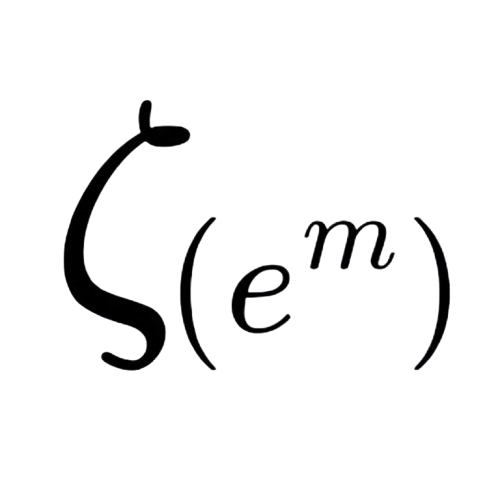
\includegraphics[width=0.7\textwidth]{cem.png} \par
    
    \vfill
    
    \textbf{Centro de Estudiantes de Matemática} \par
    2026
\end{titlepage}


\AddToShipoutPictureBG{
    \AtPageLowerLeft{
        \put(1cm,1cm){\small Centro de Estudiantes de Matemática}
    }
}

\chapter*{Prólogo}

Ante la necesidad concreta del actual período lectivo 2026, surgida directamente de la falta sistemática de material académico disponible en idioma español para el curso Análisis Real I, el Centro de Estudiantes de Matemática, en su rol de organización representativa del alumnado y principal promotor del interés estudiantil, ha tomado la iniciativa de redactar el presente material didáctico con el objetivo de serle de auténtico provecho al estudiantado en su proceso de aprendizaje y aprobación de la materia. El gremio asume esta producción para cubrir un vacío real que afecta a todos los cursantes. Una carencia material exige una respuesta organizada, y este material es la respuesta a dicha urgencia. Este material se basa explícitamente en los textos de Elon Lages Lima y Stephen Abbott.

\newpage

\tableofcontents

\newpage

\chapter{Conjuntos y Funciones}

Introduciremos en este capítulo el lenguaje de Conjuntos y Funciones, que será utilizado sistemáticamente en los capítulos siguientes. Toda la Matemática se presenta hoy en día en ese lenguaje; así, imaginamos que la mayoría de los lectores ya tenga cierta familiaridad con el tema. Sin embargo, no se exigirá conocimiento previo alguno de la materia.

\section{Conjuntos}

Un conjunto (o colección) está formado por objetos, llamados sus elementos. La relación básica entre un objeto y un conjunto es la relación de pertenencia. Cuando un objeto \( x \) es uno de los elementos que componen el conjunto \( A \), decimos que \( x \) pertenece a \( A \) y escribimos
\[ x \in A. \]

Si, en cambio, \( x \) no es uno de los elementos del conjunto \( A \), decimos que \( x \) no pertenece a \( A \) y escribimos
\[ x \notin A. \]

Un conjunto \( A \) queda definido (o determinado, o caracterizado) cuando se da una regla que permita decidir si un objeto arbitrario \( x \) pertenece o no a \( A \).

Ejemplo 1. Sea \( A \) el conjunto de los triángulos rectángulos. El conjunto \( A \) está bien definido: un objeto \( x \) pertenece a \( A \) cuando es un triángulo y, además, uno de sus ángulos es recto. Si \( x \) no es un triángulo, o si \( x \) es un triángulo que no posee ángulo recto, entonces \( x \) no pertenece a \( A \).

Se usa la notación
\[ X = \{a, b, c, \ldots\} \]
para representar el conjunto \( X \) cuyos elementos son los objetos \( a, b, c \), etc. Así, por ejemplo, \( \{1, 2\} \) es el conjunto cuyos elementos son los números 1 y 2. Dado el objeto \( a \), puede considerarse el conjunto cuyo único elemento es \( a \). Ese conjunto se representa por \( \{a\} \).

El conjunto de los números naturales 1, 2, 3, … será representado por el símbolo \( \mathbb{N} \). Por tanto
\[ \mathbb{N} = \{1, 2, 3, \ldots\}. \]

El conjunto de los números enteros (positivos, negativos y cero) será indicado por el símbolo \( \mathbb{Z} \). Así,
\[ \mathbb{Z} = \{\ldots, -3, -2, -1, 0, 1, 2, 3, \ldots\}. \]

El conjunto \( \mathbb{Q} \), de los números racionales, está formado por las fracciones \( p/q \), donde \( p \) y \( q \) pertenecen a \( \mathbb{Z} \), siendo \( q \neq 0 \). En símbolos,
\[
\mathbb{Q} = \{p/q \; ; \quad p \in \mathbb{Z}, \quad q \in \mathbb{Z}, \quad q \neq 0\}.
\]

Se lee: "\( \mathbb{Q} \) es el conjunto de las fracciones \( p/q \) tales que \( p \) pertenece a \( \mathbb{Z} \), \( q \) pertenece a \( \mathbb{Z} \) y \( q \) es diferente de cero".

La mayoría de los conjuntos encontrados en Matemática no se definen especificando, uno a uno, sus elementos. El método más frecuente para definir un conjunto es mediante una propiedad común y exclusiva de sus elementos. Más precisamente, se parte de una propiedad \( P \). Ella define un conjunto \( X \) así: si un objeto \( x \) goza de la propiedad \( P \), entonces \( x \in X \); si \( x \) no goza de \( P \), entonces \( x \notin X \). Se escribe
\[X = \{x \; ; \quad x \text{ goza de la propiedad } P\}.\]

Se lee: "\( X \) es el conjunto de los elementos \( x \) tales que \( x \) goza de la propiedad \( P \)".

Muchas veces la propiedad \( P \) se refiere a elementos de un conjunto fundamental \( E \). En este caso, se escribe
\[X = \{x \in E \; ; \quad x \text{ goza de la propiedad } P\}.\]

Por ejemplo, sea \( \mathbb{N} \) el conjunto de los números naturales y consideremos la siguiente propiedad, que se refiere a un elemento genérico \( x \in \mathbb{N} \):

"\( x \) es mayor que 5".

La propiedad \( P \), de que un número natural sea mayor que 5, define el conjunto \( X = \{6, 7, 8, 9, \dots\} \), es decir,
\[X = \{x \in \mathbb{N} \; ; \quad x > 5\}.\]

Se lee: "\( X \) es el conjunto de los \( x \) pertenecientes a \( \mathbb{N} \) tales que \( x \) es mayor que 5".

A veces ocurre que ningún elemento de \( E \) goza de la propiedad \( P \). En este caso, el conjunto \( \{x \in E \; ; \quad x \text{ goza de } P\} \) no posee ningún elemento alguno. Esto es lo que se llama un conjunto vacío Para representarlo, usaremos el símbolo \(\emptyset\).

Por lo tanto, el conjunto vacío \(\emptyset\) se define así:

Cualquiera que sea \(x\), se tiene \(x \notin \emptyset\).

Por ejemplo, tenemos \(\{x \in \mathbb{N}; 1 < x < 2\} = \emptyset\). Y también, \(\{x; x \neq x\} = \emptyset\).

Dados los conjuntos \(A\) y \(B\), decimos que \(A\) es subconjunto de \(B\) cuando todo elemento de \(A\) es también elemento de \(B\). Para indicar este hecho, se usa la notación
\[A \subset B.\]

Cuando \(A \subset B\), se dice también que \(A\) es parte de \(B\), que \(A\) está incluido en \(B\), o contenido en \(B\). La relación \(A \subset B\) se llama relación de inclusión.

Ejemplo 2. Los conjuntos numéricos \(\mathbb{N}, \mathbb{Z}\) y \(\mathbb{Q}\), presentados arriba, cumplen las relaciones de inclusión \(\mathbb{N} \subset \mathbb{Z}\) y \(\mathbb{Z} \subset \mathbb{Q}\). Abreviadamente, escribimos \(\mathbb{N} \subset \mathbb{Z} \subset \mathbb{Q}\).

Ejemplo 3. Sean \(X\) el conjunto de los cuadrados e \(Y\) el conjunto de los rectángulos. Todo cuadrado es un rectángulo, luego \(X \subset Y\).

Cuando se escribe \(X \subset Y\) no queda excluida la posibilidad de que resulte \(X = Y\). En el caso en que \(X \subset Y\) y \(X \neq Y\), se dice que \(X\) es una parte propia o un subconjunto propio de \(Y\).

Afirmar \(x \in X\) equivale a afirmar \(\{x\} \subset X\).

Para mostrar que un conjunto \(X\) no es subconjunto de un conjunto \(Y\), se debe obtener un elemento de \(X\) que no pertenezca a \(Y\). Así, por ejemplo, no se tiene \(\mathbb{Q} \subset \mathbb{Z}\), pues \(1/2 \in \mathbb{Q}\) y \(1/2\) no es entero.

De ello se sigue que el conjunto vacío \(\emptyset\) es subconjunto de cualquier conjunto \(X\). En efecto, si no fuera \(\emptyset \subset X\), existiría algún \(x \in \emptyset\) tal que \(x \notin X\). Como no existe \(x \in \emptyset\), estamos obligados a admitir que
\[\emptyset \subset X,\]

sea cual sea el conjunto \(X\).

La relación de inclusión \(A \subset B\) es:

- Reflexiva – \(A \subset A\), sea cual sea el conjunto \(A\);\\
- Antisimétrica – si \(A \subset B\) y \(B \subset A\), entonces \(A = B\);\\
- Transitiva – si \(A \subset B\) y \(B \subset C\), entonces \(A \subset C\).

La verificación de estos tres hechos es inmediata.

Se sigue de la propiedad antisimétrica que dos conjuntos \(A\) y \(B\) son iguales precisamente cuando \(A \subset B\) y \(B \subset A\), es decir, cuando poseen los mismos elementos.

Recordemos que, sean cuales fueren los significados de los símbolos \(E\) y \(D\), el signo de igualdad en una expresión como \(E = D\) significa que los símbolos \(E\) y \(D\) están siendo usados para representar el mismo objeto. En otras palabras, una cosa solo es igual a sí misma.

En el caso de conjuntos, escribir \(A = B\) significa que \(A\) y \(B\) son el mismo conjunto, o sea, que \(A\) y \(B\) poseen los mismos elementos. Siempre que tengamos que probar una igualdad entre conjuntos \(A\) y \(B\), debemos demostrar primero que \(A \subset B\) (esto es, que todo elemento de \(A\) pertenece necesariamente a \(B\)) y, después, que \(B \subset A\).

Dado un conjunto \(X\), se indica con \(\mathcal{P}(X)\) el conjunto cuyos elementos son las partes de \(X\). En otras palabras, afirmar que \(A \in \mathcal{P}(X)\) es lo mismo que decir \(A \subset X\). \(\mathcal{P}(X)\) se llama el conjunto de las partes de \(X\). Nunca es vacío: se tiene al menos \(\emptyset \in \mathcal{P}(X)\) y \(X \in \mathcal{P}(X)\).

Ejemplo 4. Sea \(X = \{1, 2, 3\}\). Entonces
\[
\mathcal{P}(X) = \{\emptyset, \{1\}, \{2\}, \{3\}, \{1, 2\}, \{1, 3\}, \{2, 3\}, X\}.
\]

Sean \(P\) y \(Q\) propiedades que se refieren a elementos de un cierto conjunto \(E\). Las propiedades \(P\) y \(Q\) definen subconjuntos \(X\) e \(Y\) de \(E\), a saber:
\[
X = \{x \in E \; ; \quad x \text{ goza de } P\} \quad \text{y} \quad Y = \{y \in E \; ; \quad y \text{ goza de } Q\}.
\]

Las afirmaciones "P implica Q", "si P, entonces Q", "P acarrea Q", "P es condición suficiente para Q", "Q es condición necesaria para P" tienen todas el mismo significado. Quieren decir que \(X \subset Y\), es decir, que todo objeto que goza de P también goza de Q. Para expresar este hecho, se usa la notación
\[
P \Rightarrow Q.
\]

También las afirmaciones "P si, y solo si, Q", "P es condición necesaria y suficiente para Q" tienen todas el mismo significado. Quieren decir que \(P \Rightarrow Q\) y \(Q \Rightarrow P\), o sea, que el conjunto \(X\) de los elementos que gozan de la propiedad \(P\) coincide con el conjunto \(Y\) de los elementos que gozan de \(Q\). La notación que expresa este hecho es
\[
P \Leftrightarrow Q.
\]

\section{Operaciones entre conjuntos}

La unión de los conjuntos \(A\) y \(B\) es el conjunto \(A \cup B\), formado por los elementos de \(A\) más los elementos de \(B\). Así, afirmar que \(x \in A \cup B\) significa decir que al menos una de las siguientes afirmaciones es verdadera: \(x \in A\) o \(x \in B\). Podemos entonces escribir:
\[
A \cup B = \{x \; ; \quad x \in A \text{ o } x \in B\}.
\]

Al contrario del lenguaje vulgar, la palabra "o" se utiliza siempre en Matemáticas en el sentido amplio: al decir "\(x \in A\) o \(x \in B\)" se quiere afirmar que al menos una de esas dos alternativas es verdadera, sin quedar excluida la posibilidad de que ambas lo sean, es decir, de tenerse al mismo tiempo \(x \in A\) y \(x \in B\).

\begin{center}
    \begin{tikzpicture}[node distance=2.5cm, thick]
        
        \def\radius{1.6}
        \def\dist{1.1}
        
        \begin{scope}
            \clip (-\dist, 0) circle (\radius) (\dist, 0) circle (\radius);
            \foreach \y in {-1.6,-1.2,...,1.6}
                \draw (-\dist-\radius, \y) -- (\dist+\radius, \y);
        \end{scope}

        \draw (-\dist, 0) circle (\radius);
        \draw (\dist, 0) circle (\radius);

        \node at (-\dist, 0) {\Large $\underline{A}$};
        \node at (\dist, 0) {\Large $\underline{B}$};

        \draw [decorate, decoration={brace, mirror, amplitude=10pt}] 
            (-\dist-\radius, -1.8) -- (\dist+\radius, -1.8) 
            node [midway, yshift=-0.8cm] {\Large $A \cup B$};

    \end{tikzpicture}
\end{center}

En la figura anterior, donde \(A\) y \(B\) son discos, la unión \(A \cup B\) es la parte sombreada.

Sean cuales fueren los conjuntos \(A\) y \(B\), se tiene \(A \subset A \cup B\) y \(B \subset A \cup B\).

La intersección de los conjuntos \(A\) y \(B\) es el conjunto \(A \cap B\), formado por los elementos comunes a \(A\) y \(B\). Así, afirmar que \(x \in A \cap B\) significa decir que se tiene, al mismo tiempo, \(x \in A\) y \(x \in B\). Escribimos entonces
\[
A \cap B = \{x \; ; \quad x \in A \text{ y } x \in B\}.
\]

Puede ocurrir que no exista elemento alguno \(x\) tal que \(x \in A\) y \(x \in B\). En este caso, se tiene \(A \cap B = \emptyset\) y los conjuntos \(A\) y \(B\) se dicen disjuntos.

\begin{center}
  \centering
  \begin{tikzpicture}[scale=0.7, transform shape, line width=1.2pt]

    \coordinate (A) at (-2,0);
    \coordinate (B) at (2,0);
    \def\rad{3.0}

    \begin{scope}
      \clip (A) circle (\rad);
      \clip (B) circle (\rad);
      
      \foreach \y in {-2.6, -2.1, ..., 2.6} {
        \draw[thin, line width=0.5pt, black] (-4, \y) -- (4, \y);
      }
    \end{scope}

    \draw (A) circle (\rad);
    \draw (B) circle (\rad);

    \node at (-3.8, 0) {\normalsize \(\underline{A}\)};
    \node at (3.8, 0) {\normalsize \(\underline{B}\)};
    
    \node at (0, 0) {\small \(\underline{A} \cap \underline{B}\)};

  \end{tikzpicture}
\end{center}

En la figura anterior, los conjuntos \(A\) y \(B\) están representados por discos y la intersección \(A \cap B\) es la parte sombreada.

Cualesquiera que sean los conjuntos \(A\) y \(B\) se tiene \(A \cap B \subset A\) y \(A \cap B \subset B\).

Ejemplo 5. Sean \(A = \{x \in \mathbb{N}; x \leq 10\}\) y \(B = \{x \in \mathbb{N}; x > 5\}\). Entonces \(A \cup B = \mathbb{N}\) y \(A \cap B = \{6, 7, 8, 9, 10\}\).

Ejemplo 6. Sean \(A = \{x \in \mathbb{N}; x > 2\}\) el conjunto de los números naturales mayores que 2, y \(B = \{x \in \mathbb{N}; x < 3\}\) el conjunto de los números naturales menores que 3. Entonces \(A \cap B = \emptyset\), pues no existen números naturales \(x\) tales que \(2 < x < 3\). Así los conjuntos \(A\) y \(B\) son disjuntos.

Relacionamos en las listas siguientes las principales propiedades formales de las operaciones de unión e intersección.

U1) \(A \cup \emptyset = A\)  \\
U2) \(A \cup A = A\)  \\
U3) \(A \cup B = B \cup A\)  \\
U4) \((A \cup B) \cup C = A \cup (B \cup C)\)  \\
U5) \(A \cup B = A \iff B \subset A\)  \\
U6) \(A \subset B,\; A' \subset B' \Rightarrow A \cup A' \subset B \cup B'\)  \\
U7) \(A \cup (B \cap C) = (A \cup B) \cap (A \cup C)\)

I1) \(A \cap \emptyset = \emptyset\)  \\
I2) \(A \cap A = A\)  \\
I3) \(A \cap B = B \cap A\)  \\
I4) \((A \cap B) \cap C = A \cap (B \cap C)\)  \\
I5) \(A \cap B = A \iff A \subset B\)  \\
I6) \(A \subset B,\; A' \subset B' \Rightarrow A \cap A' \subset B \cap B'\)  \\
I7) \(A \cap (B \cup C) = (A \cap B) \cup (A \cap C)\)

La demostración de cualquiera de estas propiedades se reduce al manejo adecuado de los conectivos "y" y "o". En realidad, podemos interpretar las propiedades anteriores como reglas formales para el manejo de esos conectivos. Demostremos una de ellas, a modo de ejemplo.

Vamos a demostrar ahora U7. Primeramente probaremos que \(A \cup (B \cap C) \subset (A \cup B) \cap (A \cup C)\). Dado \(x \in A \cup (B \cap C)\), se tiene \(x \in A\) o, entonces, \(x \in B \cap C\). En el primer caso, viene \(x \in A \cup B\) y \(x \in A \cup C\), de donde \(x \in (A \cup B) \cap (A \cup C)\). En el segundo caso tenemos \(x \in B\) y \(x \in C\). De \(x \in B\) se sigue \(x \in A \cup B\) y de \(x \in C\) se concluye \(x \in A \cup C\). Luego, \(x \in A \cup B\) y \(x \in A \cup C\), es decir, \(x \in (A \cup B) \cap (A \cup C)\). En cualquier hipótesis, \(x \in A \cup (B \cap C)\) implica \(x \in (A \cup B) \cap (A \cup C)\). Esto quiere decir: \(A \cup (B \cap C) \subset (A \cup B) \cap (A \cup C)\). Ahora mostraremos que \((A \cup B) \cap (A \cup C) \subset A \cup (B \cap C)\). Para esto, sea \(x \in (A \cup B) \cap (A \cup C)\). Entonces \(x \in A \cup B\) y \(x \in A \cup C\). Dentro de esta situación, hay dos posibilidades: o \(x \in A\) o \(x \notin A\). Si \(x \notin A\), entonces (como \(x \in A \cup B\) y \(x \in A \cup C\)) debe ser \(x \in B\) y \(x \in C\), esto es, \(x \in B \cap C\) y, por tanto, \(x \in A \cup (B \cap C)\). Si \(x \in A\) entonces evidentemente \(x \in A \cup (B \cap C)\). En cualquier hipótesis, \(x \in (A \cup B) \cap (A \cup C)\) implica \(x \in A \cup (B \cap C)\), o sea, \((A \cup B) \cap (A \cup C) \subset A \cup (B \cap C)\), como queríamos probar.

La diferencia entre los conjuntos \(A\) y \(B\) es el conjunto \(A - B\), formado por los elementos de \(A\) que no pertenecen a \(B\). En símbolos:
\[
A - B = \{x \; ; \quad x \in A \text{ y } x \notin B\}.
\]

\begin{center}
  \begin{tikzpicture}[scale=0.7, transform shape, line width=1.2pt]

    \coordinate (A) at (-2,0);
    \coordinate (B) at (2,0);
    \def\rad{3.0}

    \begin{scope}
      \clip (A) circle (\rad);
      
      \foreach \y in {-2.6, -2.1, ..., 2.6} {
        \draw[thin, line width=0.5pt, black] (-5.2, \y) -- (1, \y);
      }
      
      \fill[white] (B) circle (\rad);
    \end{scope}

    \draw (A) circle (\rad);
    \draw (B) circle (\rad);

    \node at (-2.7, 0) {\large \(\underline{A} - \underline{B}\)};

  \end{tikzpicture}
\end{center}

En la figura anterior, donde los conjuntos \(A\) y \(B\) están representados por discos, la diferencia \(A - B\) es la parte sombreada.

No se exige que \(B\) esté contenido en \(A\) para formar la diferencia \(A - B\). Cuando \(A\) y \(B\) son disjuntos, ningún elemento de \(A\) pertenece a \(B\); por tanto, \(A - B = A\). En cualquier caso, se tiene \(A - B = A - (A \cap B)\).

Cuando se tiene \(B \subset A\), la diferencia \(A - B\) se llama el complementario de \(B\) en relación con \(A\) y se escribe
\[
A - B = \mathcal{C}_A B.
\]

Frecuentemente, se tiene un conjunto \(E\) que contiene todos los conjuntos que ocurren en una cierta discusión. En este caso, la diferencia \(E - X\) se llama simplemente el complementario de \(X\) y se indica con la notación \(\mathcal{C}X\).

Por ejemplo, en los capítulos siguientes estaremos estudiando subconjuntos del conjunto \(\mathbb{R}\), de los números reales. Dado \(X \subset \mathbb{R}\), la diferencia \(\mathbb{R} - X\) será llamada el complementario de \(X\) e indicada por el símbolo \(\mathcal{C}X\), sin necesidad de mencionar explícitamente que se trata del complementario en relación con \(\mathbb{R}\).

Confirmando: si nos restringimos a considerar elementos pertenecientes a un conjunto básico \(E\), entonces
\[
x \in \mathcal{C}X \iff x \notin X.
\]

Ejemplo 7. Sean \( A = \{x \in \mathbb{Z}; x \geq -3\} \) y \( B = \{x \in \mathbb{Z}; x \leq 2\} \). Entonces \( A - B = \{x \in \mathbb{Z}; x \geq 3\} \) y \( B - A = \{x \in \mathbb{Z}; x \leq -4\} \). Tomando \(\mathbb{Z}\) como conjunto básico, entonces \( \mathcal{C}A = \{\text{enteros menores que } -3\} \) y \( \mathcal{C}B = \{\text{enteros mayores que } 2\} \).

La noción de diferencia se reduce a la de complementario del siguiente modo: dados \( A \) y \( B \), contenidos en un conjunto fundamental \( E \), respecto del cual tomamos complementarios, tenemos:
\[
A - B = A \cap \mathcal{C}B.
\]

En efecto, \( x \in A - B \Leftrightarrow x \in A \) y \( x \notin B \Leftrightarrow x \in A \) y \( x \in \mathcal{C}B \Leftrightarrow x \in A \cap \mathcal{C}B \).

Relacionamos a continuación las principales propiedades formales de la operación de tomar complementarios. Los conjuntos \( A \) y \( B \) son partes de un conjunto fundamental \( E \), en relación con el cual estamos tomando los complementarios.

C1) \( \mathcal{C}(\mathcal{C}A) = A \),\\
C2) \( A \subset B \Leftrightarrow \mathcal{C}B \subset \mathcal{C}A \),\\
C3) \( A = \emptyset \Leftrightarrow \mathcal{C}A = E \),\\
C4) \( \mathcal{C}(A \cup B) = \mathcal{C}A \cap \mathcal{C}B \),\\
C5) \( \mathcal{C}(A \cap B) = \mathcal{C}A \cup \mathcal{C}B \).

Demostraremos estas cinco propiedades.

C1) Tenemos \( x \in \mathcal{C}(\mathcal{C}A) \Leftrightarrow x \notin \mathcal{C}A \Leftrightarrow x \in A \). Luego \( \mathcal{C}(\mathcal{C}A) = A \).

C2) Supongamos \( A \subset B \). Entonces un elemento \( x \in \mathcal{C}B \) no puede pertenecer a \( B \) y, con mayor razón, no pertenecerá a \( A \). Luego \( x \in \mathcal{C}B \Rightarrow x \in \mathcal{C}A \), o sea \( \mathcal{C}B \subset \mathcal{C}A \). Recíprocamente, si tenemos \( \mathcal{C}B \subset \mathcal{C}A \) entonces, por lo que acabamos de ver, debe ser \( \mathcal{C}(\mathcal{C}A) \subset \mathcal{C}(\mathcal{C}B) \). Usando C1, obtenemos \( A \subset B \).

C3) \( A = \emptyset \Leftrightarrow x \notin A \) para todo \( x \in E \Leftrightarrow x \in \mathcal{C}A \) para todo \( x \in E \Leftrightarrow \mathcal{C}A = E \).

C4) Como \( A \subset A \cup B \) y \( B \subset A \cup B \), se sigue de C2 que \( \mathcal{C}(A \cup B) \subset \mathcal{C}A \) y \( \mathcal{C}(A \cup B) \subset \mathcal{C}B \), de donde \( \mathcal{C}(A \cup B) \subset \mathcal{C}A \cap \mathcal{C}B \). Sea \( X = \mathcal{C}A \cap \mathcal{C}B \). Tenemos \( X \subset \mathcal{C}A \) y \( X \subset \mathcal{C}B \). Por C2, viene \( A \subset \mathcal{C}X \) y \( B \subset \mathcal{C}X \), de donde \( A \cup B \subset \mathcal{C}X \). Por C2 y C1, viene \( X \subset \mathcal{C}(A \cup B) \), es decir, \( \mathcal{C}A \cap \mathcal{C}B \subset \mathcal{C}(A \cup B) \). Concluimos que \( \mathcal{C}(A \cup B) = \mathcal{C}A \cap \mathcal{C}B \).

C5) Demostración análoga a C4.

Las propiedades anteriores muestran que, tomando complementarios, se invierten las inclusiones, se transforman uniones en intersecciones y viceversa.

\begin{center}
    \centering
    \begin{tikzpicture}[scale=0.45]
        \foreach \y in {1,...,7} {
            \draw (0,\y) -- (12,\y);
        }
        \draw[thick] (0,0) rectangle (12,8);
        
        \fill[white] (6,4) circle (2.2);
        \draw[thick] (6,4) circle (2.2);
        
        \node at (6,4) {\Large $A$};
        \node[anchor=north east] at (11.8, 7.8) {\Large $E$};
    \end{tikzpicture}
    \hspace{0.5cm}
    \begin{tikzpicture}[scale=0.45]
        \draw (0,0) grid (12,8);
        
        \fill[white] (4.5,4) circle (2);
        \fill[white] (7.5,4) circle (2);
        
        \begin{scope}
            \clip (4.5,4) circle (2);
            \foreach \x in {1,...,11} {
                \draw (\x,0) -- (\x,8);
            }
        \end{scope}
        
        \begin{scope}
            \clip (7.5,4) circle (2);
            \foreach \y in {1,...,7} {
                \draw (0,\y) -- (12,\y);
            }
        \end{scope}
        
        \begin{scope}
            \clip (4.5,4) circle (2);
            \fill[white] (7.5,4) circle (2);
        \end{scope}
        
        \draw[thick] (0,0) rectangle (12,8);
        \draw[thick] (4.5,4) circle (2);
        \draw[thick] (7.5,4) circle (2);
        
        \node at (3.8,4) {\Large $A$};
        \node at (8.2,4) {\Large $B$};
    \end{tikzpicture}
\end{center}

En la figura de la izquierda, \( A \) es un disco, contenido en el rectángulo, que es el conjunto fundamental \( E \). El complementario de \( A \) es la parte sombreada con líneas horizontales. En la figura de la derecha, \( A \) y \( B \) son discos. El complementario de \( A \) está sombreado con líneas horizontales y el complementario de \( B \) con líneas verticales. Entonces \( \mathcal{C}(A \cup B) \) es la parte cuadriculada, mientras que \( \mathcal{C}(A \cap B) \) es la parte que tiene algún tipo de línea (vertical, horizontal o ambas). Esto muestra que \( \mathcal{C}(A \cup B) = \mathcal{C}A \cap \mathcal{C}B \) y \( \mathcal{C}(A \cap B) = \mathcal{C}A \cup \mathcal{C}B \).

Otra operación útil entre conjuntos es el producto cartesiano. Se basa en el concepto de par ordenado, que discutiremos ahora.

Dados los objetos \( a, b \), el par ordenado \( (a, b) \) queda formado cuando se elige uno de esos objetos (a saber: \( a \)) para ser la primera coordenada del par y (consecuentemente) el objeto \( b \) para ser la segunda coordenada del par. Dos pares ordenados \( (a, b) \) y \( (a', b') \) serán llamados iguales cuando sus primeras coordenadas, \(a\) y \(a'\), sean iguales y sus segundas coordenadas, \(b\) y \(b'\), también. Así
\[
(a, b) = (a', b') \iff a = a' \text{ y } b = b'.
\]

No se debe confundir el par ordenado \((a, b)\) con el conjunto \(\{a, b\}\). En efecto, como dos conjuntos que poseen los mismos elementos son iguales, tenemos \(\{a, b\} = \{b, a\}\), sean cuales fueren \(a\) y \(b\). Por otro lado, por la definición de igualdad entre pares ordenados solo tenemos \((a, b) = (b, a)\) cuando \(a = b\). Notemos además que \(\{a, a\} = \{a\}\), mientras que \((a, a)\) es un par ordenado legítimo.

El producto cartesiano de los conjuntos \(A\) y \(B\) es el conjunto \(A \times B\) cuyos elementos son todos los pares ordenados \((a, b)\) cuya primera coordenada pertenece a \(A\) y la segunda a \(B\). Por tanto:
\[
A \times B = \{(a, b) \; ; \quad a \in A \text{ y } b \in B\}.
\]

Cuando \(A = B\), tenemos el producto cartesiano \(A^2 = A \times A\). El subconjunto \(\Delta \subset A \times A\), formado por los pares \((a, a)\) cuyas coordenadas son iguales, se llama la diagonal de \(A^2\).

\begin{center}
    \centering
    \begin{tikzpicture}[scale=0.75]

        \begin{scope}[shift={(0,0)}]
            \draw[thick] (0,0) rectangle (7,5);
            \node[anchor=north east] at (6.8, 4.8) {$A \times B$};

            \draw (-0.5, 0.5) -- (-0.5, 5.5);
            \node[anchor=south] at (-0.5, 5.5) {$B$};
            \draw (0.5, -0.5) -- (7.5, -0.5);
            \node[anchor=west] at (7.5, -0.5) {$A$};

            \node[circle, fill, inner sep=1.2pt] (a_axis_a) at (1.5, -0.5) {};
            \node[anchor=north] at (1.5, -0.5) {$a$};
            \node[circle, fill, inner sep=1.2pt] (a_axis_b) at (-0.5, 3.5) {};
            \node[anchor=east] at (-0.5, 3.5) {$b$};

            \node[circle, fill, inner sep=1.2pt] (a_pt) at (1.5, 3.5) {};
            \node[anchor=west] at (1.5, 3.5) {$(a,b)$};

            \draw[dashed] (1.5, 3.5) -- (1.5, -0.5);
            \draw[dashed] (1.5, 3.5) -- (-0.5, 3.5);
        \end{scope}

        \begin{scope}[shift={(9.5,0)}]
            \draw[thick] (0,0) rectangle (5,5);

            \draw (-0.5, 0.5) -- (-0.5, 5.5);
            \node[anchor=south] at (-0.5, 5.5) {$A$};
            \draw (0.5, -0.5) -- (5.5, -0.5);
            \node[anchor=west] at (5.5, -0.5) {$A$};

            \draw[thick] (0,0) -- (5,5);
            \node[anchor=west] at (2.5, 2.5) {$\Delta$};

            \node[circle, fill, inner sep=1.2pt] (b_axis_a_horiz) at (1.5, -0.5) {};
            \node[anchor=north] at (1.5, -0.5) {$a$};
            \node[circle, fill, inner sep=1.2pt] (b_axis_a_vert) at (-0.5, 1.5) {};
            \node[anchor=east] at (-0.5, 1.5) {$a$};
            \node[circle, fill, inner sep=1.2pt] (b_axis_aprime_vert) at (-0.5, 3.5) {};
            \node[anchor=east] at (-0.5, 3.5) {$a'$};

            \node[circle, fill, inner sep=1.2pt] (b_pt_aa) at (1.5, 1.5) {};
            \node[anchor=west] at (1.5, 1.5) {$(a,a)$};
            \node[circle, fill, inner sep=1.2pt] (b_pt_aap) at (1.5, 3.5) {};
            \node[anchor=west] at (1.5, 3.5) {$(a,a')$};

            \draw[dashed] (1.5, 3.5) -- (1.5, -0.5); 
            \draw[dashed] (1.5, 3.5) -- (-0.5, 3.5);
            \draw[dashed] (1.5, 1.5) -- (-0.5, 1.5);
        \end{scope}

    \end{tikzpicture}
\end{center}

En la figura de la izquierda, los conjuntos \(A\) y \(B\) están representados por segmentos y el producto cartesiano \(A \times B\) por un rectángulo. A la derecha, tenemos el cuadrado \(A \times A = A^2\), en el cual se destaca la diagonal \(\Delta\).

Ejemplo 8. Sean \(A = \{1, 2, 3\}\) y \(B = \{x, y\}\). Entonces  
\[A \times B = \{(1, x), (1, y), (2, x), (2, y), (3, x), (3, y)\}\]

Ejemplo 9. La introducción de coordenadas cartesianas en el plano hace que cada punto sea representado por un par ordenado \((x, y)\), donde \(x\) es su abscisa e \(y\) su ordenada. Esto identifica el plano con el producto cartesiano \(\mathbb{R}^2 = \mathbb{R} \times \mathbb{R}\), donde \(\mathbb{R}\) es el conjunto de los números reales.

\section{Funciones}

Una función \(f: A \to B\) consta de tres partes: un conjunto \(A\), llamado el dominio de la función (o el conjunto donde la función está definida), un conjunto \(B\), llamado el codominio de la función, o el conjunto donde la función toma valores, y una regla que permite asociar, de modo bien determinado, a cada elemento \(x \in A\), un único elemento \(f(x) \in B\), llamado el valor que la función asume en \(x\) (o en el punto \(x\)).

Se usa la notación \(x \mapsto f(x)\) para indicar que \(f\) hace corresponder a \(x\) el valor \(f(x)\).

Muchas veces se dice "la función \(f\)" en lugar de "la función \(f: A \to B\)". En este caso, quedan sobrentendidos el conjunto \(A\), dominio de \(f\), y el conjunto \(B\), codominio de \(f\).

No se debe confundir \(f\) con \(f(x)\): \(f\) es la función, mientras que \(f(x)\) es el valor que la función asume en un punto \(x\) de su dominio.

La naturaleza de la regla que enseña cómo obtener el valor \(f(x) \in B\) cuando se da \(x \in A\) es enteramente arbitraria, estando sujeta solo a dos condiciones:

\begin{enumerate}
\item No debe haber excepciones: para que \(f\) tenga el conjunto \(A\) como dominio, la regla debe proporcionar \(f(x)\) para todo \(x \in A\);

\item No debe haber ambigüedades: a cada \(x \in A\), la regla debe hacer corresponder un único \(f(x)\) en \(B\).
\end{enumerate}

Vemos que no existen funciones "plurívocas". Por la segunda condición, arriba, si \(x = y\) en \(A\), entonces \(f(x) = f(y)\) en \(B\).

Se deduce de las consideraciones anteriores que dos funciones \(f: A \to B\) y \(g: A' \to B'\) son iguales si, y solo si, \(A = A'\), \(B = B'\) y \(f(x) = g(x)\) para todo \(x \in A\). Es decir, dos funciones son iguales cuando tienen el mismo dominio, el mismo codominio y la misma regla de correspondencia.

Ejemplo 10. Sea \(P\) el conjunto de los polígonos del plano, \(\mathbb{R}\) el conjunto de los números reales y \(f: P \to \mathbb{R}\) la función que asocia a cada polígono \(x\) su área \(f(x)\).

Ejemplo 11. Sean \(A = B = \mathbb{Q}\). Intentemos definir una función \(f: \mathbb{Q} \to \mathbb{Q}\) considerando la siguiente regla: a cada número \(x \in \mathbb{Q}\), hagamos corresponder el número \(f(x) \in \mathbb{Q}\) tal que \(x \cdot f(x) = 1\). Esta regla no define una función de \(\mathbb{Q}\) en \(\mathbb{Q}\), pues dado \(0 \in \mathbb{Q}\), no existe número racional alguno \(y = f(0)\) tal que \(0 \cdot y = 1\). Sin embargo, si elegimos el conjunto \(A = \mathbb{Q} - \{0\}\) como dominio, la misma regla define la función \(f: A \to \mathbb{Q}\), \(f(x) = 1/x\).

Ejemplo 12. Sea \(T\) el conjunto de los triángulos del plano y \(\mathbb{R}^+\) el conjunto de los números reales positivos. Consideremos el intento de definir una función \(f: \mathbb{R}^+ \to T\) mediante la siguiente regla: a cada número real \(x > 0\) hagamos corresponder el triángulo \(f(x)\) cuya área es \(x\). Evidentemente, hay ambigüedades: dado un número real \(x > 0\), existe una infinidad de triángulos cuyo área es \(x\). La regla no define una función.

El gráfico de una función \(f: A \to B\) es el subconjunto \(G(f)\) del producto cartesiano \(A \times B\) formado por los pares ordenados \((x, f(x))\), donde \(x \in A\) es arbitrario. Es decir,
\[
G(f) = \{(x, y) \in A \times B \; ; \quad y = f(x)\}.
\]

Se sigue de la definición de igualdad entre funciones que dos funciones son iguales si, y solo si, poseen el mismo gráfico.

Para que un subconjunto \(G \subset A \times B\) sea el gráfico de una función \(f: A \to B\), es necesario y suficiente que, para cada \(x \in A\), exista un único punto \((x, y) \in G\) cuya primera coordenada sea \(x\). Para funciones \(f: A \to B\), donde \(A\) y \(B\) son conjuntos de números reales, esta condición significa que toda paralela al eje de las ordenadas, trazada por un punto de \(A\), debe cortar al gráfico \(G\) en uno y solo un punto.

\begin{center}
\begin{tikzpicture}

    \draw[thick] (0,0) rectangle (4.5, 3);
    \node at (3.8, 2.6) {$A \times B$};

    \draw[thick] (0,-0.5) -- (4.5,-0.5) node[below] {$A$};
    \draw[thick] (-0.4,0) -- (-0.4,3) node[left] {$B$};

    \draw[thick] (0, 1.1) .. controls (0.2, 1.8) and (0.4, 2.3) .. (0.8, 2.3)
                 .. controls (1.2, 2.3) and (1.8, 1.1) .. (2.8, 1.0)
                 .. controls (3.6, 0.9) and (4.1, 1.3) .. (4.5, 1.5);
                 
    \node at (3.7, 1.15) [above] {$G(f)$};

    \coordinate (x_val) at (0.8, -0.5);
    \coordinate (y_val) at (-0.4, 2.3);
    \coordinate (p_val) at (0.8, 2.3);

    \draw[dashed] (x_val) -- (p_val) -- (y_val);

    \fill (x_val) circle (1.5pt) node[below] {$x$};
    \fill (y_val) circle (1.5pt) node[left] {$f(x)$};
    \fill (p_val) circle (1.5pt) node[above right=-1pt] {$(x,f(x))$};

    \begin{scope}[xshift=5.8cm]

        \draw[thick] (0,0) rectangle (4.5, 3);
        \node at (3.8, 2.6) {$A \times B$};

        \draw[thick] (0,-0.5) -- (4.5,-0.5) node[below] {$A$};
        \draw[thick] (-0.4,0) -- (-0.4,3) node[left] {$B$};

        \draw[thick] (0,2.2)
                     .. controls (0.8, 2.6) and (1.4, 3.1) .. (1.3, 2.4)
                     .. controls (1.2, 1.8) and (0.8, 2.3) .. (0.8, 1.8)
                     .. controls (0.8, 1.3) and (1.6, 1.5) .. (2.2, 1.6)
                     .. controls (3.0, 1.7) and (3.8, 2.3) .. (3.5, 1.6)
                     .. controls (3.3, 1.0) and (3.0, 1.4) .. (3.1, 1.0)
                     .. controls (3.2, 0.6) and (4.0, 1.1) .. (4.5, 1.8);

    \end{scope}

\end{tikzpicture}
\end{center}

En la figura de la izquierda tenemos el gráfico de una función \(f: A \to B\). La figura de la derecha muestra un subconjunto de \(A \times B\) que no puede ser gráfico de una función de \(A\) en \(B\).

Una función \(f: A \to B\) se llama inyectiva (o biunívoca) cuando, dados \(x, y\) cualesquiera en \(A\), \(f(x) = f(y)\) implica \(x = y\). En otras palabras: cuando \(x \neq y\) en \(A\) implica \(f(x) \neq f(y)\) en \(B\).

El ejemplo más simple de una función inyectiva es la inclusión \(i: A \to B\), definida cuando \(A\) es un subconjunto de \(B\), por la regla \(i(x) = x\), para todo \(x \in A\).

Una función \(f: A \to B\) se llama sobreyectiva (o sobre \(B\)) cuando, para todo \(y \in B\) existe al menos un \(x \in A\) tal que \(f(x) = y\).

Ejemplos de funciones sobreyectivas son las proyecciones \(\pi_1: A \times B \to A\) y \(\pi_2: A \times B \to B\), de un producto cartesiano \(A \times B\) en los factores \(A\) y \(B\), respectivamente. La primera proyección, \(\pi_1\), se define por \(\pi_1(a, b) = a\), mientras que la segunda proyección, \(\pi_2\), se define por \(\pi_2(a, b) = b\).

Ejemplo 13. Sea \(f: \mathbb{Z} \to \mathbb{Z}\) definida por \(f(x) = x^2\). Entonces \(f\) no es inyectiva, pues \(f(-3) = f(3)\), aunque \(-3 \neq 3\). Tampoco \(f\) es sobreyectiva, pues no existe \(x \in \mathbb{Z}\) tal que \(x^2 = -1\). Por otro lado, si tomamos \(g: \mathbb{Z} \to \mathbb{Z}\), definida por \(g(x) = 3x + 1\), entonces \(g\) es inyectiva. De hecho, si \( g(x) = g(y) \) entonces \( 3x + 1 = 3y + 1 \), o sea, \( 3x = 3y \), de donde \( x = y \). Pero \( g \) no es sobreyectiva, pues no existe un entero \( x \) tal que \( 3x + 1 = 0 \), por ejemplo. Finalmente, sea \( h: \mathbb{N} \to \mathbb{N} \) definida así: \( h(1) = 1 \) y, para cada número natural \( x > 1 \), \( h(x) \) es el número de factores primos distintos que entran en la composición de \( x \). Entonces \( h \) es sobreyectiva, pues \( h(2) = 1 \), \( h(6) = 2 \), \( h(30) = 3 \), \( h(210) = 4 \), etc. Pero es claro que \( h \) no es inyectiva. Por ejemplo, si \( x \) e \( y \) son dos números primos cualesquiera, se tiene \( h(x) = h(y) \).

Ejemplo 14. La verificación de que una función es sobreyectiva implica demostrar la existencia de objetos que satisfacen ciertas condiciones. Por ejemplo, sea \( \mathbb{R}^+ \) el conjunto de los números reales positivos. Consideremos la función \( f: \mathbb{R} \to \mathbb{R}^+ \), definida por \( f(x) = x^2 \). Decir que \( f \) es sobreyectiva significa afirmar que, para todo número real \( y > 0 \) existe algún número real \( x \) tal que \( y = x^2 \), o sea, que todo número real positivo \( y \) posee una raíz cuadrada \( x \). (Esto será probado cuando estudiemos los números reales.) Otro ejemplo: sea \( p \) un polinomio no constante, de coeficientes complejos. A cada número complejo \( z \) asociemos el valor \( p(z) \) del polinomio \( p \). Esto define una función \( p: \mathbb{C} \to \mathbb{C} \), donde \( \mathbb{C} \) es el conjunto de los números complejos. La afirmación de que \( p \) es una función sobreyectiva es equivalente al llamado "Teorema Fundamental del Álgebra" (un teorema de Topología, según el cual todo polinomio complejo no constante posee al menos una raíz compleja). En efecto, admitiendo que \( p: \mathbb{C} \to \mathbb{C} \) es sobreyectiva, dado \( 0 \in \mathbb{C} \), debe existir algún \( z \in \mathbb{C} \) tal que \( p(z) = 0 \). El número \( z \) es, por tanto, una raíz de \( p \). Recíprocamente, admitiendo que todo polinomio no constante posee una raíz compleja, probamos que \( p: \mathbb{C} \to \mathbb{C} \) es sobreyectiva. En efecto, dado \( c \in \mathbb{C} \), la función \( z \mapsto p(z) - c \) es un polinomio no constante, luego existe algún \( z_0 \in \mathbb{C} \) tal que \( p(z_0) - c = 0 \). Se tiene \( p(z_0) = c \), de donde \( p \) es sobreyectiva.

Una función \( f: A \to B \) se llama biyectiva (una biyección, o una correspondencia biunívoca) cuando es inyectiva y sobreyectiva al mismo tiempo.

La más simple de las biyecciones es la función identidad \(\text{id}_A: A \to A\), definida por \(\text{id}_A(x) = x\), para todo \(x \in A\). Cuando no haya peligro de confusión, escribiremos simplemente \(\text{id}: A \to A\), en lugar de \(\text{id}_A\).

Por ejemplo, dados arbitrariamente \(a, b\) en \(\mathbb{Q}\), con \(a \neq 0\), la función \(f: \mathbb{Q} \to \mathbb{Q}\), definida por \(f(x) = ax + b\), es una biyección. En efecto, si \(f(x) = f(y)\), es decir, \(ax + b = ay + b\) entonces, sumando \(-b\) a ambos miembros, viene \(ax = ay\). Multiplicando ambos miembros por \(1/a\), obtenemos \(x = y\). Así, \(f\) es inyectiva. Además, dado \(y \in \mathbb{Q}\) cualquiera, el número racional \(x = (y - b)/a\) es tal que \(ax + b = y\), esto es, \(f(x) = y\), de donde \(f\) es sobreyectiva.

Dadas una función \(f: A \to B\) y una parte \(X \subset A\), se llama imagen de \(X\) por la función \(f\) al conjunto \(f(X)\) formado por los valores \(f(x)\) que \(f\) asume en los puntos \(x \in X\). Así
\[
f(X) = \{f(x) \; ; \quad x \in X\} = \{y \in B \; ; \quad y = f(x), \; x \in X\}.
\]

Evidentemente, \(f(X)\) es un subconjunto de \(B\). Para que \(f: A \to B\) sea sobreyectiva es necesario y suficiente que \(f(A) = B\). En general, se tiene solo \(f(A) \subset B\). El conjunto \(f(A)\) se llama la imagen de la función \(f\). A veces también se dice que \(f(A)\) es el conjunto de los valores de \(f\).

Dada una función \(f: A \to B\) e indicando con \(X, Y, \dots\) subconjuntos de \(A\), tenemos

I1) \(f(X \cup Y) = f(X) \cup f(Y)\),  \\
I2) \(f(X \cap Y) \subset f(X) \cap f(Y)\),  \\
I3) \(X \subset Y \Rightarrow f(X) \subset f(Y)\),  \\
I4) \(f(\emptyset) = \emptyset\).

Demostremos las dos primeras de estas relaciones.

I1) Si \(y \in f(X \cup Y)\), entonces existe \(x \in X \cup Y\) tal que \(f(x) = y\). Si \(x \in X\), tenemos \(y \in f(X)\). Si, en cambio, \(x \in Y\), tenemos \(y \in f(Y)\). En cualquier caso, \(y \in f(X) \cup f(Y)\). Luego \(f(X \cup Y) \subset f(X) \cup f(Y)\). Recíprocamente, sea \(z \in f(X) \cup f(Y)\). Entonces \(z \in f(X)\) o \(z \in f(Y)\). En el primer caso, existe \(x \in X\) tal que \(z = f(x)\). En el segundo, existe \(y \in Y\) tal que \(z = f(y)\). En cualquier hipótesis, existe \(w \in X \cup Y\) tal que \(z = f(w)\). Así \(z \in f(X \cup Y)\), esto es, \(f(X) \cup f(Y) \subset f(X \cup Y)\). Estas dos inclusiones muestran que \(f(X \cup Y) = f(X) \cup f(Y)\).

I2) Si \(y \in f(X \cap Y)\) entonces existe \(x \in X \cap Y\) tal que \(f(x) = y\). Entonces \(x \in X\) y por tanto \(y \in f(X)\). También \(x \in Y\) y por tanto \(y \in f(Y)\). Luego \(y \in f(X) \cap f(Y)\).

Ejemplo 15. Sea \(\mathbb{R}\) el conjunto de los números reales. Definimos \(f: \mathbb{R} \to \mathbb{R}\) poniendo \(f(x) = x^2\). Entonces la imagen de \(f\), o sea, el conjunto \(f(\mathbb{R})\), es el conjunto de los números reales \(\geq 0\). (Aquí estamos haciendo uso del hecho, que se demostrará más adelante, de que todo número real positivo posee una raíz cuadrada).

Ejemplo 16. Sea \(f: A \to B\) una función que no es inyectiva. Entonces existen \(x \neq y\) en \(A\), con \(f(x) = f(y)\). Pongamos \(X = \{x\}\) e \(Y = \{y\}\). Se tiene \(X \cap Y = \emptyset\), luego \(f(X \cap Y) = \emptyset\). Sin embargo \(f(X) \cap f(Y) = \{f(x)\}\) no es vacío. Luego, en este caso, tenemos \(f(X \cap Y) \neq f(X) \cap f(Y)\).

Si, en cambio, \(f: A \to B\) es inyectiva, podemos probar que \(f(X \cap Y) = f(X) \cap f(Y)\) para cualesquiera \(X, Y\) contenidos en \(A\).

En efecto, dado \(y \in f(X) \cap f(Y)\), tenemos \(y \in f(X)\) e \(y \in f(Y)\). Luego existen \(x' \in X\) y \(x'' \in Y\) con \(y = f(x')\) y \(y = f(x'')\). Como \(f\) es inyectiva, debe ser \(x' = x''\) y por tanto \(x' \in X \cap Y\). Se sigue que \(y = f(x')\) pertenece a \(f(X \cap Y)\), lo que muestra que \(f(X) \cap f(Y) \subset f(X \cap Y)\). Como la inclusión opuesta es siempre verdadera, concluimos que \(f(X \cap Y) = f(X) \cap f(Y)\).

En resumen, para que se tenga \(f(X \cap Y) = f(X) \cap f(Y)\) para cualesquiera \(X, Y\) contenidos en \(A\), es necesario y suficiente que la función \(f: A \to B\) sea inyectiva.

Dada una función \(f: A \to B\), consideremos un conjunto \(Y \subset B\). La imagen inversa de \(Y\) por la función \(f\) es el conjunto \(f^{-1}(Y)\), formado por todos los \(x \in A\) tales que \(f(x) \in Y\). Así:
\[
f^{-1}(Y) = \{x \in A \; ; \quad f(x) \in Y\}.
\]

Nótese que puede ocurrir \(f^{-1}(Y) = \emptyset\) incluso si \(Y \subset B\) es un subconjunto no vacío. Esto sucede precisamente cuando \(Y \cap f(A) = \emptyset\), es decir, cuando \(Y\) no tiene puntos en común con la imagen de \(f\). En particular, \(f\) no es sobreyectiva. Dado \(y \in B\), escribimos \(f^{-1}(y)\) en lugar de \(f^{-1}(\{y\})\). Puede ocurrir que \(f^{-1}(y)\) posea más de un elemento, pues \(f\) puede no ser inyectiva.

Ejemplo 17. Los subconjuntos del plano definidos en Geometría Analítica mediante ecuaciones y desigualdades son imágenes inversas de conjuntos. Por ejemplo, la recta que tiene la ecuación \(ax + by = c\) es el conjunto \(X = \{(x, y) \in \mathbb{R}^2 \; ; \quad ax + by = c\}\). Consideremos la función \(f: \mathbb{R}^2 \to \mathbb{R}\), definida por \(f(x, y) = ax + by\). Entonces la recta \(X\) es la imagen inversa del conjunto \(\{c\}\) por \(f\), o sea, \(X = f^{-1}(c)\). También la circunferencia cuya ecuación es \(x^2 + y^2 = 1\) (centro en el origen y radio 1) es el conjunto \(C = \{(x, y) \in \mathbb{R}^2 \; ; \quad x^2 + y^2 = 1\}\). Tomemos la función \(g: \mathbb{R}^2 \to \mathbb{R}\), definida por \(g(x, y) = x^2 + y^2\). Tenemos \(C = g^{-1}(1)\).

Ahora consideremos el disco \(D\) de centro en el origen y radio 1. Tenemos \(D = \{(x, y) \in \mathbb{R}^2 \; ; \quad x^2 + y^2 \leq 1\}\). Sea \(g: \mathbb{R}^2 \to \mathbb{R}\), nuevamente, la función definida por \(g(x, y) = x^2 + y^2\). Tomemos el intervalo \(I = [0, 1] = \{t \in \mathbb{R} \; ; \quad 0 \leq t \leq 1\}\). Entonces el disco \(D\) es la imagen inversa del intervalo \(I\) por la función \(g\): \(D = g^{-1}(I)\).

Las imágenes inversas se comportan bien relativamente a las operaciones con conjuntos. En la relación siguiente, \(Y\) y \(Z\) indican subconjuntos de \(B\). Dada una función \(f: A \to B\), tenemos

Inv1) \(f^{-1}(Y \cup Z) = f^{-1}(Y) \cup f^{-1}(Z)\),\\
Inv2) \(f^{-1}(Y \cap Z) = f^{-1}(Y) \cap f^{-1}(Z)\),\\
Inv3) \(f^{-1}(\mathcal{C}Y) = \mathcal{C} f^{-1}(Y)\),\\
Inv4) \(Y \subset Z \Rightarrow f^{-1}(Y) \subset f^{-1}(Z)\),\\
Inv5) \(f^{-1}(B) = A\),\\
Inv6) \(f^{-1}(\emptyset) = \emptyset\).

Vamos a demostrar las tres primeras.

Inv1) Tenemos \(x \in f^{-1}(Y \cup Z) \iff f(x) \in Y \cup Z \iff f(x) \in Y\) o \(f(x) \in Z \iff x \in f^{-1}(Y)\) o \(x \in f^{-1}(Z) \iff x \in f^{-1}(Y) \cup f^{-1}(Z)\).

Inv2) \(x \in f^{-1}(Y \cap Z) \iff f(x) \in Y \cap Z \iff f(x) \in Y\) y \(f(x) \in Z \iff x \in f^{-1}(Y)\) y \(x \in f^{-1}(Z) \iff x \in f^{-1}(Y) \cap f^{-1}(Z)\).

Inv3) \(x \in f^{-1}(\mathcal{C}Y) \iff f(x) \in \mathcal{C}Y \iff f(x) \notin Y \iff x \notin f^{-1}(Y) \iff x \in \mathcal{C} f^{-1}(Y)\).

\section{Composición de funciones}

Sean \(f: A \to B\) y \(g: B \to C\) funciones tales que el dominio de \(g\) es igual al codominio de \(f\). En este caso, podemos definir la función compuesta \(g \circ f: A \to C\), que consiste en aplicar primero \(f\) y después \(g\). Más precisamente,
\[
(g \circ f)(x) = g(f(x)) \quad \text{para todo } x \in A.
\]

Dadas \(f: A \to B\), \(g: B \to C\) y \(h: C \to D\), vale la ley asociativa
\[
(h \circ g) \circ f = h \circ (g \circ f): A \to D.
\]
En efecto, para todo \(x \in A\), tenemos:
\[
[(h \circ g) \circ f](x) = (h \circ g)(f(x)) = h[g(f(x))] = h[(g \circ f)(x)] = [h \circ (g \circ f)](x).
\]

Observamos que, más generalmente, basta que la imagen \(f(A)\) de la función \(f\) esté contenida en el dominio de \(g\) para que la definición \((g \circ f)(x) = g(f(x))\) tenga sentido y proporcione la función compuesta \(g \circ f: A \to C\).

Si \(f: A \to B\) y \(g: B \to C\) son inyectivas, entonces \(g \circ f: A \to C\) es inyectiva. También la compuesta de funciones sobreyectivas es sobreyectiva. En particular, la compuesta de dos biyecciones es una biyección. Estos hechos son de verificación inmediata.

Por otro lado, cualquier función \(f: A \to B\) puede escribirse como compuesta \(f = h \circ f_1\) de una función inyectiva \(h\) con una función sobreyectiva. Basta considerar \(f_1: A \to f(A)\), definida por \(f_1(x) = f(x)\), y la inclusión \(h: f(A) \to B\).

También podemos escribir cualquier función \(f: A \to B\) como compuesta \(f = \pi \circ F\) de una función sobreyectiva \(\pi\) con una función inyectiva \(F\). Basta tomar \(F: A \to A \times B\), donde \(F(x) = (x, f(x))\) y \(\pi: A \times B \to B\), con \(\pi(x, y) = y\) (segunda proyección).

Sean \(f: A \to B\) y \(g: B \to C\) funciones. Dado \(X \subset A\), se tiene \((g \circ f)(X) = g(f(X))\). Si \(Z \subset C\), tenemos \((g \circ f)^{-1}(Z) = f^{-1}(g^{-1}(Z))\).

Probemos esta última relación. Para \(x \in A\), tenemos:

\begin{align*}
x \in f^{-1}(g^{-1}(Z)) &\iff f(x) \in g^{-1}(Z) \\
&\iff g(f(x)) \in Z \\
&\iff (g \circ f)(x) \in Z \\
&\iff x \in (g \circ f)^{-1}(Z)
\end{align*}

La restricción de una función \(f: A \to B\) a un subconjunto \(X \subset A\) es la función \(f|_X: X \to B\), definida por \((f|_X)(x) = f(x)\) para todo \(x \in X\). Considerando la inclusión \(i: X \to A\), tenemos \(f|_X = f \circ i: X \to B\).

Dado \(X \subset A\), si \(g: X \to B\) es la restricción de una función \(f: A \to B\) al conjunto \(X\), se dice también que \(f\) es una extensión de \(g\). Extender una función \(g: X \to B\) al conjunto \(A \supset X\) es, por tanto, obtener una función \(f: A \to B\) que coincida con \(g\) en \(X\), esto es, tal que \(f|_X = g\). Evidentemente hay, en general, diversas extensiones de la misma función \(g\).

Un gran número de problemas matemáticos importantes se reducen a extender una o varias funciones de modo que las extensiones satisfagan ciertas condiciones adicionales (continuidad, analiticidad, etc.). La función que se desea extender se llama la "condición de contorno".

Dadas las funciones \(f: A \to B\) y \(g: B \to A\), diremos que \(g\) es una inversa a la izquierda para \(f\) cuando \(g \circ f = \text{id}_A: A \to A\), es decir, cuando \(g(f(x)) = x\) para todo \(x \in A\).

Por ejemplo, sean \(A\) el conjunto de los números reales \(\geq 0\) y \(\mathbb{R}\) el conjunto de todos los números reales. Consideremos \(f: A \to \mathbb{R}\), definida por \(f(x) = x^2\), y \(g: \mathbb{R} \to A\), definida por \(g(y) = \sqrt{y}\) si \(y \geq 0\) y \(g(y) = 0\) si \(y < 0\). Para todo \(x \in A\), tenemos \(g(f(x)) = g(x^2) = \sqrt{x^2} = x\). Luego \(g \circ f = \text{id}_A\) y, por tanto, \(g\) es una inversa a la izquierda de \(f\). Nótese que cualquier función \(h: \mathbb{R} \to A\), tal que \(h(y) = \sqrt{y}\) para \(y \geq 0\), es una inversa a la izquierda de \(f\). (La definición de los valores \(h(y)\) para \(y < 0\) puede ser cualquiera, sin que quede afectada la igualdad \(h \circ f = \text{id}_A\)).

Una función \(f: A \to B\) posee inversa a la izquierda si, y solo si, es inyectiva.

\textbf{Demostración}. Si \(f\) es inyectiva, para cada \(y \in f(A)\) existe un único \(x \in A\) tal que \(y = f(x)\). Escribamos \(x = g(y)\). Esto define una función \(g: f(A) \to A\) tal que \(g(f(x)) = x\) para todo \(x \in A\). Completamos la definición de \(g: B \to A\) poniendo, por ejemplo, \(g(y) = x_0\) (elemento que fijamos en \(A\)) para \(y \in B - f(A)\). Obtenemos \(g: B \to A\) tal que \(g \circ f = \text{id}_A\). Recíprocamente, si existe \(g: B \to A\) tal que \(g \circ f = \text{id}_A\) entonces, dados \(x', x''\) en \(A\), \(f(x') = f(x'') \Rightarrow x' = g(f(x')) = g(f(x'')) = x''\), y por tanto, \(f\) es inyectiva.

Una función \(g: B \to A\) se llama inversa a la derecha de una función \(f: A \to B\) cuando \(f \circ g = \text{id}_B: B \to B\), es decir, cuando \(f(g(y)) = y\) para todo \(y \in B\).

Por ejemplo, sea \(f: \mathbb{N} \to \mathbb{N}\) definida por \(f(1) = 1\) y, si \(x > 1\), \(f(x) =\) número de factores primos distintos que entran en la composición de \(x\). Definamos \(g: \mathbb{N} \to \mathbb{N}\) poniendo \(g(y) =\) menor número natural que es el producto de \(y\) factores primos distintos. Entonces, para todo número natural \(y\), tenemos \(f(g(y)) = y\). Luego \(f \circ g = \text{id}_{\mathbb{N}}\) y, por tanto, \(g\) es una inversa a la derecha para \(f\). Otras funciones \(h: \mathbb{N} \to \mathbb{N}\) podrían definirse con la propiedad \(f \circ h = \text{id}_{\mathbb{N}}\). Por ejemplo, podríamos poner \(h(y) =\) menor número natural divisible por 13 que es el producto de \(y\) factores primos distintos.

Una función \(f: A \to B\) posee inversa a la derecha si, y solo si, es sobreyectiva.

\textbf{Demostración}. Sea \(f: A \to B\) sobreyectiva. Entonces, para cada \(y \in B\), el conjunto \(f^{-1}(y)\) no es vacío. Elijamos, para cada \(y \in B\), un \(x \in A\) tal que \(f(x) = y\) y pongamos \(g(y) = x\). Esto define una función \(g: B \to A\) tal que \(f(g(y)) = y\). Luego \(g\) es una inversa a la derecha de \(f\). Recíprocamente, si existe \(g: B \to A\) con \(f \circ g = \text{id}_B\) entonces, para cada \(y \in B\), poniendo \(x = g(y)\), tenemos \(f(x) = f(g(y)) = y\). Luego \(f\) es sobreyectiva.

Una función \(g: B \to A\) se llama inversa de la función \(f: A \to B\) cuando \(g \circ f = \text{id}_A\) y \(f \circ g = \text{id}_B\), es decir, cuando \(g\) es inversa a izquierda y a la derecha para \(f\).

Por ejemplo, sea \(a\) un número racional \(\neq 0\) y definamos \(f: \mathbb{Q} \to \mathbb{Q}\) poniendo \(f(x) = ax\). La función \(g: \mathbb{Q} \to \mathbb{Q}\), definida por \(g(x) = x/a\), es inversa de \(f\).

Otro ejemplo: dada una función arbitraria \(f: A \to B\), sea \(G(f)\) el gráfico de \(f\). (Recordemos que \(G(f)\) es el subconjunto de \(A \times B\) formado por los pares ordenados \((x, f(x))\), donde \(x\) recorre \(A\).) Definimos una función \(F: A \to G(f)\) poniendo \(F(x) = (x, f(x))\). Sea \(\pi: G(f) \to A\) definida por \(\pi(x, f(x)) = x\). (Evidentemente, \(\pi = \pi_1 |_{G(f)}\) es la restricción a \(G(f)\) de la primera proyección \(\pi_1: A \times B \to A\).) Entonces \(F \circ \pi = \text{id}_{G(f)}\) y \(\pi \circ F = \text{id}_A\), como se ve fácilmente. Por tanto \(\pi\) es inversa de \(F\).

Se sigue de las dos proposiciones anteriores que una función \(f: A \to B\) posee inversa si, y solo si, es una biyección.

Al contrario de las inversas de un solo lado, si una función \(f: A \to B\) posee una inversa, ella es única.

En efecto, supongamos que \(g: B \to A\) y \(h: B \to A\) sean ambas inversas de \(f\). Entonces \(h = h \circ \text{id}_B = h \circ (f \circ g) = (h \circ f) \circ g = \text{id}_A \circ g = g\).

El lector atento habrá notado que probamos arriba un poco más de lo enunciado, a saber: si \(f\) posee una inversa a la izquierda, \(h\), y una inversa a la derecha, \(g\), entonces \(h = g\) y \(f\) tiene una inversa.

Escribiremos \(f^{-1}: B \to A\) para indicar la inversa de la biyección \(f: A \to B\).

Evidentemente, si \(f: A \to B\) y \(g: B \to C\) son biyecciones, se tiene \((g \circ f)^{-1} = f^{-1} \circ g^{-1}\).

\section{Familias}

Una familia es una función cuyo valor en un punto \(x\) se indica con \(f_x\) en lugar de \(f(x)\).

Pasemos a las definiciones formales.
Sea \(L\) un conjunto, cuyos elementos llamaremos índices y representaremos genéricamente por \(\lambda\).

Dado un conjunto \(X\), una familia de elementos de \(X\) con índices en \(L\) es una función \(x: L \to X\). El valor de \(x\) en el punto \(\lambda \in L\) se indicará con el símbolo \(x_\lambda\), en lugar de la notación usual \(x(\lambda)\). La familia \(x\) se representa por la notación \((x_\lambda)_{\lambda \in L}\) o simplemente \((x_\lambda)\) cuando no haya duda sobre el conjunto de índices \(L\).

Tomemos, por ejemplo, \(L = \{1, 2\}\) como conjunto de índices. Dado un conjunto \(X\), una familia de elementos de \(X\) con índices en \(L\) es una función \(x: \{1, 2\} \to X\). Los valores de esta función en los puntos 1 y 2 se representan por \(x_1\) y \(x_2\). Se obtiene así un par ordenado \((x_1, x_2)\) de elementos de \(X\). Recíprocamente, todo par ordenado \((x_1, x_2)\) de elementos de \(X\) es una familia \(x: \{1, 2\} \to X\). En suma, los pares ordenados de elementos de \(X\) son las familias de elementos de \(X\) con índices en el conjunto \(L = \{1, 2\}\). Es decir, el producto cartesiano \(X^2 = X \times X\) es el conjunto de las funciones (familias) \(x: \{1, 2\} \to X\). Más generalmente, dados los conjuntos \(X_1\) y \(X_2\), el producto cartesiano \(X_1 \times X_2\) es el conjunto de las familias \(x: \{1, 2\} \to X_1 \cup X_2\) tales que \(x_1 \in X_1\) y \(x_2 \in X_2\).

Cuando \(L = \{1, 2, \dots, n\}\) es el conjunto de los números naturales desde 1 hasta \(n\), una familia \(x: L \to X\) se llama una \(n\)-upla de elementos de \(X\). Una \(n\)-upla \(x = (x_i)_{i \in L}\) se representa comúnmente por la notación \(x = (x_1, \dots, x_n)\). El elemento \(x_i\) se llama la \(i\)-ésima coordenada de la \(n\)-upla \(x = (x_1, \dots, x_n)\).

Sea \((A_\lambda)_{\lambda \in L}\) una familia de conjuntos con índices en \(L\). (Esto quiere decir: a cada \(\lambda \in L\) hacemos corresponder un conjunto \(A_\lambda\).) La unión de esa familia es el conjunto de los elementos que pertenecen al menos a uno de los conjuntos \(A_\lambda\). Se representa por la notación \(\bigcup_{\lambda \in L} A_\lambda\) o, simplemente, \(\bigcup A_\lambda\). Así
\[
\bigcup_{\lambda \in L} A_\lambda = \{x \; ; \quad \text{existe } \lambda \in L \text{ con } x \in A_\lambda\}.
\]

En otras palabras, \(\bigcup A_\lambda\) es el conjunto de los elementos que pertenecen a algún \(A_\lambda\).

Análogamente, la intersección de la familia \((A_\lambda)_{\lambda \in L}\) es el conjunto de los elementos que pertenecen simultáneamente a todos los \(A_\lambda\).

Notación: \(\bigcap_{\lambda \in L} A_\lambda\) o simplemente \(\bigcap A_\lambda\). Por tanto,
\[
\bigcap_{\lambda \in L} A_\lambda = \{x \; ; \quad x \in A_\lambda \text{ para todo } \lambda \in L\}.
\]

Cuando \(L = \{1, 2, \dots, n\}\), se escribe
\[
\bigcup_{i \in L} A_i = \bigcup_{i=1}^n A_i = A_1 \cup \cdots \cup A_n,
\]
\[
\bigcap_{i \in L} A_i = \bigcap_{i=1}^n A_i = A_1 \cap \cdots \cap A_n.
\]

Una familia con índices en el conjunto \(\mathbb{N} = \{1, 2, \dots\}\) de los números naturales se llama una sucesión. Así, una sucesión \(x = (x_n)_{n \in \mathbb{N}} = (x_1, x_2, \dots, x_n, \dots)\) de elementos de un conjunto \(X\) es una función \(x: \mathbb{N} \to X\), donde el valor \(x(n)\) se indica con el símbolo \(x_n\) y se llama el n-ésimo término de la sucesión.

Dada una sucesión de conjuntos \((A_n)_{n \in \mathbb{N}}\), su unión y su intersección se representan por
\[
\bigcup_{n \in \mathbb{N}} A_n = \bigcup_{n=1}^\infty A_n = A_1 \cup A_2 \cup \cdots \cup A_n \cup \cdots,
\]
\[
\bigcap_{n \in \mathbb{N}} A_n = \bigcap_{n=1}^\infty A_n = A_1 \cap A_2 \cap \cdots \cap A_n \cap \cdots.
\]

Ejemplo 18. Para cada \(n \in \mathbb{N}\), consideremos el conjunto
\[
A_n = \{-n, -n+1, \dots, -1, 0, 1, \dots, n-1, n\}.
\]

Entonces
\[
\bigcup_{n=1}^\infty A_n = \mathbb{Z} \quad \text{y} \quad \bigcap_{n=1}^\infty A_n = \{-1, 0, 1\},
\]

como se ve fácilmente.

Dada una familia \((A_\lambda)_{\lambda \in L}\) de subconjuntos de un conjunto fundamental \(E\), se tiene
\[
\mathcal{C}\left(\bigcup A_\lambda\right) = \bigcap \mathcal{C} A_\lambda
\]
y
\[
\mathcal{C}\left(\bigcap A_\lambda\right) = \bigcup \mathcal{C} A_\lambda.
\]

En efecto, dado \(x \in E\), tenemos sucesivamente \(x \in \mathcal{C}(\bigcup A_\lambda) \iff x \notin \bigcup A_\lambda \iff\) no existe \(\lambda \in L\) tal que \(x \in A_\lambda \iff x \notin A_\lambda\) para todo \(\lambda \in L \iff x \in \mathcal{C} A_\lambda\) para todo \(\lambda \in L \iff x \in \bigcap \mathcal{C} A_\lambda\).

Esto prueba la primera igualdad. La segunda es consecuencia, teniendo en cuenta que \(\mathcal{C}(\mathcal{C}X) = X\). En efecto, si escribimos \(\mathcal{C} A_\lambda = B_\lambda\), tenemos \(\mathcal{C} B_\lambda = A_\lambda\). Luego
\[
\mathcal{C}\left(\bigcap A_\lambda\right) = \mathcal{C}\left(\bigcap \mathcal{C} B_\lambda\right) = \mathcal{C}\left(\mathcal{C}\left(\bigcup B_\lambda\right)\right) = \bigcup B_\lambda = \bigcup \mathcal{C} A_\lambda.
\]

Ejemplo 19. Sea \((A_\lambda)_{\lambda \in L}\) una familia de subconjuntos de un conjunto \(E\). Afirmar que \(\bigcup A_\lambda = E\) equivale a decir que, para todo elemento \(x \in E\) existe al menos un \(\lambda \in L\) tal que \(x \in A_\lambda\). Sea \(B_\lambda = \mathcal{C} A_\lambda\). Se tiene \(\bigcup A_\lambda = E\) si, y solo si, la intersección de los \(B_\lambda\) es vacía, esto es, \(\bigcap B_\lambda = \emptyset\). En efecto, por lo que vimos \(\bigcap B_\lambda = \mathcal{C}(\bigcup A_\lambda)\).

Dada una función \(f: A \to B\), consideremos una familia \((A_\lambda)_{\lambda \in L}\) de subconjuntos de \(A\), y una familia \((B_\mu)_{\mu \in M}\) de subconjuntos de \(B\). Se tiene
\[
f\left(\bigcup A_\lambda\right) = \bigcup f(A_\lambda),
\]
\[
f\left(\bigcap A_\lambda\right) \subset \bigcap f(A_\lambda),
\]
\[
f^{-1}\left(\bigcup B_\mu\right) = \bigcup f^{-1}(B_\mu),
\]
\[
f^{-1}\left(\bigcap B_\mu\right) = \bigcap f^{-1}(B_\mu).
\]

Probemos la primera y la última de estas afirmaciones. Dado \(y \in B\), tenemos:

\[
y \in f\left(\bigcup A_\lambda\right) \iff \text{existe } x \in \bigcup A_\lambda \text{ tal que } y = f(x)
\]
\[
\iff \text{existen } \lambda \in L \text{ y } x \in A_\lambda \text{ con } y = f(x)
\]
\[
\iff \text{existe } \lambda \in L \text{ tal que } y \in f(A_\lambda)
\]
\[
\iff y \in \bigcup f(A_\lambda).
\]

Dado \( x \in A \), tenemos
\[
x \in f^{-1}(\cap B_\mu) \iff f(x) \in \cap B_\mu \iff f(x) \in B_\mu \text{ para todo } \mu \in M
\]
\[
\iff x \in f^{-1}(B_\mu) \text{ para todo } \mu \in M \iff x \in \cap f^{-1}(B_\mu).
\]

La noción de familia permite considerar productos cartesianos de una cantidad arbitraria de conjuntos.

Dados los conjuntos \( A_1, \ldots, A_n \), su producto cartesiano
\[
A = A_1 \times \cdots \times A_n = \prod_{i=1}^n A_i
\]

es el conjunto formado por todas las \( n \)-uplas \( a = (a_1, \ldots, a_n) \) tales que \( a_1 \in A_1, \ldots, a_n \in A_n \).

En otras palabras, \( A_1 \times \cdots \times A_n \) es el conjunto de todas las funciones \( a : \{1, 2, \ldots, n\} \to A_1 \cup A_2 \cup \cdots \cup A_n \) tales que \( a(i) = a_i \in A_i \) para \( i = 1, 2, \ldots, n \).

Esta definición extiende la del producto cartesiano \( A \times B \).

Cuando \( A_1 = \cdots = A_n = A \), el producto cartesiano \( A \times \cdots \times A \) de \( n \) copias de \( A \) se indica con \( A^n \). Consiste en todas las funciones \( a : \{1, 2, \ldots, n\} \to A \), es decir, de todas las \( n \)-uplas de elementos de \( A \).

En el producto cartesiano \( A = A_1 \times \cdots \times A_n \), destacan las proyecciones \( \pi_1 : A \to A_1 \), \( \pi_2 : A \to A_2, \ldots, \pi_n : A \to A_n \). La \( i \)-ésima proyección \( \pi_i : A \to A_i \) se define poniendo \( \pi_i(a) = a_i = i \)-ésima coordenada de la \( n \)-upla \( a = (a_1, \ldots, a_n) \). Dados \( a = (a_1, \ldots, a_n) \) y \( b = (b_1, \ldots, b_n) \) en \( A_1 \times \cdots \times A_n \), se tiene \( a = b \) si, y solo si, \( \pi_i(a) = \pi_i(b) \) para cada \( i = 1, \ldots, n \).

Sea \( X \subset A_1 \times \cdots \times A_n \). Los elementos \( x = (x_1, \ldots, x_n) \) de \( X \) poseen \( n \) coordenadas. Las funciones \( f : X \to B \), definidas en \( X \), pueden ser pensadas como funciones de \( n \) variables (la primera variable estando en \( A_1 \), la segunda en \( A_2 \), etc.) En particular, introduciendo coordenadas cartesianas en el plano, este se identifica con el producto cartesiano \( \mathbb{R}^2 = \mathbb{R} \times \mathbb{R} \). Las funciones \( f : X \to \mathbb{R} \), definidas en subconjuntos \( X \subset \mathbb{R}^2 \), son las funciones reales de dos variables reales.

Dada una familia de conjuntos \( (A_\lambda)_{\lambda \in L} \), su producto cartesiano
\[
A = \prod_{\lambda \in L} A_\lambda
\]

es el conjunto de las familias \((a_\lambda)_{\lambda \in L}\) tales que, para cada \(\lambda \in L\), se tiene \(a_\lambda \in A_\lambda\).

En otras palabras, \(A\) es el conjunto de todas las funciones \(a: L \to \bigcup A_\lambda\) tales que \(a(\lambda) = a_\lambda \in A_\lambda\) para cada \(\lambda \in L\).

Las proyecciones \(\pi_\lambda: A \to A_\lambda\) se definen por \(\pi_\lambda(a) = a_\lambda\). Cada proyección \(\pi_\lambda\) es una función sobreyectiva. Dada una función \(f: X \to \prod A_\lambda\), de un conjunto cualquiera \(X\) en el producto cartesiano de los \(A_\lambda\), se obtiene, para cada \(\lambda \in L\), una función \(f_\lambda: X \to A_\lambda\), dada por \(f_\lambda = \pi_\lambda \circ f\). Así, \(f(x) = (f_\lambda(x))_{\lambda \in L}\) para cada \(x \in X\). Recíprocamente, si se da, para cada \(\lambda \in L\), una función \(f_\lambda: X \to A_\lambda\), entonces existe una única \(f: X \to \prod A_\lambda\) tal que \(f_\lambda = \pi_\lambda \circ f\) para cada \(\lambda \in L\). Basta poner \(f(x) = (f_\lambda(x))_{\lambda \in L}\) para cada \(x \in X\). Las funciones \(f_\lambda\) se llaman las coordenadas de \(f\).

En el caso particular en que todos los conjuntos \(A_\lambda\) son iguales al mismo conjunto \(A\), se escribe \(A^L\) en lugar de \(\prod_{\lambda \in L} A_\lambda\). \(A^L\) es, por tanto, el conjunto de todas las funciones de \(L\) en \(A\).

Se destaca, en especial, el producto cartesiano de una sucesión de conjuntos \(A_1, A_2, \dots, A_n, \dots\), el cual se representa con las notaciones
\[
\prod_{n \in \mathbb{N}} A_n = \prod_{n=1}^{\infty} A_n = A_1 \times A_2 \times \cdots \times A_n \times \dots
\]

Los elementos de este conjunto son las sucesiones \(a = (a_1, a_2, \dots, a_n, \dots)\) sujetas a la condición de que \(a_n \in A_n\) para todo \(n \in \mathbb{N}\).

\textbf{Ejercicios}

1. Dados los conjuntos \(A\) y \(B\), sea \(X\) un conjunto con las siguientes propiedades:

\begin{itemize}
\item[] \(1^\text{a}\) \(X \supset A\) y \(X \supset B\),
\item[] \(2^\text{a}\) Si \(Y \supset A\) y \(Y \supset B\) entonces \(Y \supset X\).
\end{itemize}

Probar que \(X = A \cup B\).

2. Enuncie y demuestre un resultado análogo al anterior, caracterizando \( A \cap B \).

3. Sean \( A, B \subset E \). Pruebe que \( A \cap B = \emptyset \) si, y solo si, \( A \subset \mathcal{C}B \). Pruebe también que \( A \cup B = E \) si, y solo si, \( \mathcal{C}A \subset B \).

4. Dados \( A, B \subset E \), pruebe que \( A \subset B \) si, y solo si, \( A \cap \mathcal{C}B = \emptyset \).

5. Dé ejemplo de conjuntos \( A, B, C \) tales que \( (A \cup B) \cap C \neq A \cup (B \cap C) \).

6. Si \( A, X \subset E \) son tales que \( A \cap X = \emptyset \) y \( A \cup X = E \), pruebe que \( X = \mathcal{C}A \).

7. Si \( A \subset B \), entonces \( B \cap (A \cup C) = (B \cap C) \cup A \) para todo conjunto \( C \). Por otro lado, si existe \( C \) de modo que la igualdad anterior sea satisfecha, entonces \( A \subset B \).

8. Pruebe que \( A = B \) si, y solo si, \( (A \cap \mathcal{C}B) \cup (\mathcal{C}A \cap B) = \emptyset \).

9. Pruebe que \( (A - B) \cup (B - A) = (A \cup B) - (A \cap B) \).

10. Sea \( A \Delta B = (A - B) \cup (B - A) \). Pruebe que \( A \Delta B = A \Delta C \) implica \( B = C \). Examine la validez de un resultado análogo con \( \cap, \cup \) o \( \times \) en lugar de \( \Delta \).

11. Pruebe las siguientes afirmaciones:

a) \( (A \cup B) \times C = (A \times C) \cup (B \times C) \);\\
b) \( (A \cap B) \times C = (A \times C) \cap (B \times C) \);\\
c) \( (A - B) \times C = (A \times C) - (B \times C) \);\\
d) \( A \subset A', B \subset B' \Rightarrow A \times B \subset A' \times B' \).

12. Dada la función \( f: A \to B \):

a) Pruebe que se tiene \( f(X - Y) \supset f(X) - f(Y) \), sean cuales fueren los subconjuntos \( X \) e \( Y \) de \( A \);\\
b) Muestre que si \(f\) es inyectiva entonces \(f(X - Y) = f(X) - f(Y)\) para cualesquiera \(X, Y\) contenidos en \(A\).

13. Muestre que la función \(f: A \to B\) es inyectiva si, y solo si, \(f(A - X) = f(A) - f(X)\) para todo \(X \subset A\).

14. Dada la función \(f: A \to B\), pruebe:

a) \(f^{-1}(f(X)) \supset X\) para todo \(X \subset A\);\\
b) \(f\) es inyectiva si, y solo si, \(f^{-1}(f(X)) = X\) para todo \(X \subset A\).

15. Dada \(f: A \to B\), pruebe:

a) para todo \(Z \subset B\), se tiene \(f(f^{-1}(Z)) \subset Z\);\\
b) \(f\) es sobreyectiva si, y solo si, \(f(f^{-1}(Z)) = Z\) para todo \(Z \subset B\).

16. Dada una familia de conjuntos \((A_\lambda)_{\lambda \in L}\), sea \(X\) un conjunto con las siguientes propiedades:

\begin{itemize}
\item[] 1ª) para todo \(\lambda \in L\), se tiene \(X \supset A_\lambda\);

\item[] 2ª) Si \(Y \supset A_\lambda\) para todo \(\lambda \in L\), entonces \(Y \supset X\).
\end{itemize}

Pruebe que, en estas condiciones, se tiene \(X = \bigcup_{\lambda \in L} A_\lambda\).

17. Enuncie y demuestre un resultado análogo al anterior, caracterizando \(\bigcap_{\lambda \in L} A_\lambda\).

18. Sea \(f: \mathcal{P}(A) \to \mathcal{P}(A)\) una función tal que \(X \subset Y \Rightarrow f(Y) \subset f(X)\) y \(f(f(X)) = X\). Pruebe que \(f(\bigcup X_\lambda) = \bigcap f(X_\lambda)\) y \(f(\bigcap X_\lambda) = \bigcup f(X_\lambda)\). [Aquí \(X, Y\) y cada \(X_\lambda\) son subconjuntos de \(A\)].

19. Dadas las familias \((A_\lambda)_{\lambda \in L}\) y \((B_\mu)_{\mu \in M}\), forme dos familias con índices en \(L \times M\) considerando los conjuntos
\[
(A_\lambda \cup B_\mu)_{(\lambda, \mu) \in L \times M} \quad \text{y} \quad (A_\lambda \cap B_\mu)_{(\lambda, \mu) \in L \times M}.
\]
Pruebe que se tiene
\[
\left( \bigcup_{\lambda \in L} A_\lambda \right) \cap \left( \bigcup_{\mu \in M} B_\mu \right) = \bigcup_{(\lambda,\mu) \in L \times M} (A_\lambda \cap B_\mu),
\]
\[
\left( \bigcap_{\lambda \in L} A_\lambda \right) \cup \left( \bigcap_{\mu \in M} B_\mu \right) = \bigcap_{(\lambda,\mu) \in L \times M} (A_\lambda \cup B_\mu).
\]

20. Sea \((A_{ij})_{(i,j) \in \mathbb{N} \times \mathbb{N}}\) una familia de conjuntos con índices en \(\mathbb{N} \times \mathbb{N}\). Pruebe, o refute mediante un contraejemplo, la igualdad
\[
\bigcup_{j=1}^{\infty} \left( \bigcap_{i=1}^{\infty} A_{ij} \right) = \bigcap_{i=1}^{\infty} \left( \bigcup_{j=1}^{\infty} A_{ij} \right).
\]

21. Dados los conjuntos \(A, B, C\), establezca una biyección entre \(\mathcal{F}(A \times B; C)\) y \(\mathcal{F}(A; \mathcal{F}(B; C))\).

\newpage

\chapter{Conjuntos Finitos, Enumerables y No Enumerables}

Una vez que tenemos los conceptos generales y los hechos básicos sobre conjuntos y funciones, los aplicaremos, en este capítulo, para estudiar las nociones de conjunto finito y conjunto infinito.

A Cantor se debe el descubrimiento fundamental de que hay diversos tipos de infinito, así como el análisis de esos tipos.

La noción de conjunto enumerable está estrictamente ligada al conjunto \(\mathbb{N}\) de los números naturales. Por ello iniciaremos este capítulo con una breve presentación de la teoría de los números naturales a partir de los axiomas de Peano.

Los axiomas de Peano exhiben los números naturales como "números ordinales", es decir, objetos que ocupan lugares determinados en una secuencia ordenada: 1 es el primer número natural, 2 es el número que viene justo después del 1, 3 viene a continuación del 2, etc. Pero los números naturales también pueden ocurrir como “Números cardinales”, es decir, como resultado de una operación de conteo, en respuesta a la pregunta: ¿cuántos elementos tiene este conjunto?

En el §2, empleamos los números naturales para el conteo de los conjuntos finitos, mostrando cómo pueden ser considerados como números cardinales y completando, por tanto, su descripción.

Una exposición sistemática de los sistemas numéricos utilizados en el Análisis Matemático puede hacerse a partir de los números naturales, mediante sucesivas extensiones del concepto de número: primero se amplía \(\mathbb{N}\) para obtener el conjunto \(\mathbb{Z}\) de los números enteros; luego se extiende \(\mathbb{Z}\), pasando al conjunto \(\mathbb{Q}\) de los números racionales; de este se pasa al conjunto \(\mathbb{R}\) de los reales y, de ahí, al conjunto \(\mathbb{C}\) de los complejos. Esta elaboración, aunque instructiva, es un proceso lento.

\section{Números naturales}

Toda la teoría de los números naturales puede deducirse de los tres axiomas siguientes, conocidos como axiomas de Peano.

Se dan, como objetos no definidos, un conjunto \(\mathbb{N}\), cuyos elementos se llaman números naturales, y una función \(s: \mathbb{N} \to \mathbb{N}\). Para cada \(n \in \mathbb{N}\), el número \(s(n)\), valor que la función asume en el punto \(n\), se llama el sucesor de \(n\).

La función \(s\) satisface los siguientes axiomas:

P1. \(s: \mathbb{N} \to \mathbb{N}\) es inyectiva. En otros términos: \(m, n \in \mathbb{N}\), \(s(m) = s(n) \Rightarrow m = n\). O, en palabras, dos números que tienen el mismo sucesor son iguales.

P2. \(\mathbb{N} - s(\mathbb{N})\) consta de un solo elemento. Es decir, existe un único número natural que no es sucesor de ningún otro. Ese se llama “uno” y se representa con el símbolo 1. Así, cualquiera que sea \(n \in \mathbb{N}\), se tiene \(1 \neq s(n)\). Por otro lado, si \(n \neq 1\) entonces existe un (único) \(n_0 \in \mathbb{N}\) tal que \(s(n_0) = n\).

P3. (Principio de Inducción). Si \(X \subset \mathbb{N}\) es un subconjunto tal que \(1 \in X\) y, para todo \(n \in X\) se tiene también \(s(n) \in X\), entonces \(X = \mathbb{N}\).

El Principio de Inducción puede también enunciarse de la siguiente manera:

Sea \(\mathcal{P}\) una propiedad referente a números naturales. Si 1 goza de la propiedad \(\mathcal{P}\) y si, del hecho de que un número natural \(n\) goce de \(\mathcal{P}\) se puede concluir que \(n + 1\) goza de la propiedad \(\mathcal{P}\), entonces todos los números naturales gozan de esa propiedad.

Una demostración en la que se emplea el axioma P3 se llama una demostración por inducción.

Para dar un ejemplo de demostración por inducción, mostremos que para todo \(n \in \mathbb{N}\) se tiene \(s(n) \neq n\). En efecto, sea \(X = \{n \in \mathbb{N}; s(n) \neq n\}\). Se tiene \(1 \in X\), pues 1 no es sucesor de ningún número, en particular \(1 \neq s(1)\). Además, \(n \in X \Rightarrow n \neq s(n) \Rightarrow\) (por la inyectividad de \(s\)) \(s(n) \neq s[s(n)] \Rightarrow s(n) \in X\). Así, \(n \in X \Rightarrow s(n) \in X\). Como \(1 \in X\), se sigue del axioma P3 que \(X = \mathbb{N}\), o sea \(n \neq s(n)\) para todo \(n \in \mathbb{N}\).

El Principio de Inducción es muy útil para demostrar proposiciones que se refieren a enteros. Él está implícito en todos los argumentos donde se dice “y así sucesivamente”, “y así seguidamente” o “etc.”.

No menos importante que demostrar proposiciones por inducción es saber definir objetos inductivamente.

Las definiciones por inducción se basan en la posibilidad de iterar una función \(f: X \to X\) un número arbitrario \(n\) de veces.

Más precisamente, sea \(f: X \to X\) una función cuyo dominio y codominio son el mismo conjunto \(X\). A cada \(n \in \mathbb{N}\) podemos, de modo único, asociar una función \(f^n: X \to X\) de tal manera que \(f^1 = f\) y \(f^{s(n)} = f \circ f^n\). En particular, si llamamos \(2 = s(1)\), \(3 = s(2)\), tendremos \(f^2 = f \circ f\), \(f^3 = f \circ f \circ f\).

En una exposición sistemática de la teoría de los números naturales, la existencia de la \(n\)-ésima iterada \(f^n\) de una función \(f: X \to X\) es un teorema, llamado “Teorema de la Definición por Inducción”. No daremos su demostración aquí. Solo observaremos que no nos sería posible, a estas alturas, definir \(f^n\) simplemente como \(f \circ f \circ \cdots \circ f\) (\(n\) veces) pues “\(n\) veces” es una expresión sin sentido en el contexto de los axiomas de Peano, ya que un número natural \(n\) es, por ahora, solo un elemento del conjunto \(\mathbb{N}\) (un número ordinal), sin condiciones de servir de respuesta a la pregunta “¿cuántas veces?”, hasta que se le otorgue la condición de número cardinal.

Admitamos, por tanto, que, dada una función \(f: X \to X\), sabemos asociar, de modo único, a cada número natural \(n \in \mathbb{N}\), una función \(f^n: X \to X\), llamada la \(n\)-ésima iterada de \(f\), de tal modo que \(f^1 = f\) y \(f^{s(n)} = f \circ f^n\).

Veamos un ejemplo de definición por inducción. Usando las iteradas de la función \(s: \mathbb{N} \to \mathbb{N}\), definiremos la suma de números naturales. Dados \(m, n \in \mathbb{N}\), su suma \(m + n \in \mathbb{N}\) se define por:
\[m + n = s^n(m).\]

Así, sumar \(m\) con 1 es tomar el sucesor de \(m\) mientras que, en general, sumar \(m\) con \(n\) es partir de \(m\) e iterar \(n\) veces la operación de tomar el sucesor. En otras palabras, tenemos, por definición:
\[m + 1 = s(m),\]
\[m + s(n) = s(m + n).\]

Así, si queremos, podremos prescindir de la notación \(s(n)\) para indicar el sucesor de \(n\) y usar la notación definitiva \(n + 1\) para representar dicho sucesor. Esto se hará gradualmente. Con la notación definitiva, la última de las igualdades anteriores se lee:
\[m + (n + 1) = (m + n) + 1.\]

Vemos que la propia definición de la suma \(m + n\) ya contiene una indicación de que goza de la propiedad asociativa. Probaremos ahora, en general, que se tiene:
\[m + (n + p) = (m + n) + p,\]

cualesquiera que sean \(m\), \(n\), \(p \in \mathbb{N}\).

La demostración de la propiedad asociativa se hace así: sea \(X\) el conjunto de los números naturales \(p\) tales que \(m + (n + p) = (m + n) + p\), cualesquiera que sean \(m\), \(n \in \mathbb{N}\). Ya vimos que \(1 \in X\). Además, si \(p \in X\), entonces,
\[m + (n + s(p)) = m + s(n + p) = s(m + (n + p)) = s((m + n) + p) = (m + n) + s(p).\]

(En el tercer signo de igualdad, usamos la hipótesis \(p \in X\) y en los demás la definición de suma.) Luego, \(p \in X \Rightarrow s(p) \in X\). Como \(1 \in X\), concluimos, por inducción, que \(X = \mathbb{N}\), es decir, \(m + (n + p) = (m + n) + p\), cualesquiera que sean \(m\), \(n\), \(p \in \mathbb{N}\).

Las propiedades formales de la adición se relacionan a continuación:

Asociatividad: \(m + (n + p) = (m + n) + p\);\\
Conmutatividad: \(m + n = n + m\);\\
Ley de cancelación: \(m + n = m + p \Rightarrow n = p\);\\
Tricotomía: dados \(m\), \(n \in \mathbb{N}\), exactamente una de las tres alternativas siguientes puede ocurrir: o \(m = n\), o existe \(p \in \mathbb{N}\) tal que \(m = n + p\), o bien existe \(q \in \mathbb{N}\) con \(n = m + q\).

Omitimos las demostraciones de esas propiedades, que se hacen por inducción.

La relación de orden entre los números naturales se define en términos de la adición. Dados los números naturales \(m\), \(n\) decimos que \(m\) es menor que \(n\) y escribimos
\[m < n,\]

para significar que existe \(p \in \mathbb{N}\) tal que \(n = m + p\). En las mismas condiciones, decimos que \(n\) es mayor que \(m\) y escribimos \(n > m\). La notación \(m \leq n\) significa que \(m\) es menor o igual que \(n\).

La relación \(<\) goza de las siguientes propiedades:

Transitividad: si \(m < n\) y \(n < p\) entonces \(m < p\).\\
Tricotomía: dados \(m\), \(n\), exactamente una de las siguientes alternativas puede ocurrir: o \(m = n\), o \(m < n\) o \(n < m\).\\
Monotonicidad de la adición: si \(m < n\) entonces, para todo \(p \in \mathbb{N}\) se tiene \(m + p < n + p\).

Probemos la última: \(m < n\) significa que existe \(q \in \mathbb{N}\) tal que \(m + q = n\). Entonces \((m + p) + q = n + p\), y, por tanto, \(m + p < n + p\).

Observemos que \(m < n\) significa que, para cierto \(p \in \mathbb{N}\), tenemos \(n = s^p(m)\), esto es, \(n\) es el sucesor del sucesor ... del sucesor de \(m\).

Introduciremos ahora la multiplicación de números naturales.

Así, como la suma \(m + n\) fue definida como el resultado que se obtiene cuando se itera \(n\) veces, a partir de \(m\), la operación de tomar el sucesor, definiremos el producto \(m \cdot n\) como la suma de \(n\) sumandos iguales a \(m\), o mejor, el resultado que se obtiene cuando se añade a \(m\), \(n - 1\) veces, el mismo número \(m\).

En términos precisos, para cada \(m \in \mathbb{N}\), sea \(f_m: \mathbb{N} \to \mathbb{N}\) la función definida por \(f_m(p) = p + m\). (Es decir, \(f_m\) es la función “sumar \(m\)”). Usaremos esta función para definir la multiplicación de números naturales.

El producto de dos números naturales se define así, \(m \cdot 1 = m\) y \(m \cdot (n + 1) = (f_m)^n(m)\).

En palabras: multiplicar un número \(m\) por 1 no lo altera. Multiplicar \(m\) por un número mayor que 1, es decir, por un número de la forma \(n+1\), es iterar \(n\) veces la operación de sumar \(m\), comenzando con \(m\). Así, por ejemplo, \(m \cdot 2 = f_m(m) = m+m\), \(m \cdot 3 = (f_m)^2(m) = m + m + m\).

Recordando la definición de \((f_m)^n\), vemos que el producto \(m \cdot n\) está definido inductivamente por las propiedades siguientes:
\[
m \cdot 1 = m,
\]
\[
m \cdot (n + 1) = m \cdot n + m.
\]

La última igualdad anterior ya sugiere que el producto debe gozar de la propiedad distributiva
\[
m \cdot (n + p) = m \cdot n + m \cdot p.
\]

Demostremos este hecho. Sea \(X\) el conjunto de los números \(p \in \mathbb{N}\) tales que \((m + n) \cdot p = m \cdot p + n \cdot p\) cualesquiera que sean \(m, n \in \mathbb{N}\). Acabamos de observar que \(1 \in X\). Además, si \(p \in X\), concluiremos que
\[
(m + n) \cdot (p + 1) = (m + n) \cdot p + m + n
\]
\[
= m \cdot p + n \cdot p + m + n = m \cdot p + m + n \cdot p + n
\]
\[
= m \cdot (p + 1) + n \cdot (p + 1).
\]

(En las igualdades anteriores usamos, sucesivamente, la definición de producto, la hipótesis de que \(p \in X\), la asociatividad y la conmutatividad de la adición y, nuevamente, la definición de producto).

Se sigue que \(p + 1 \in X\). Así, \(X = \mathbb{N}\), es decir, \((m + n) \cdot p = m \cdot p + n \cdot p\), cualesquiera que sean \(m, n, p \in \mathbb{N}\).

Las principales propiedades de la multiplicación son:

Asociatividad: \(m \cdot (n \cdot p) = (m \cdot n) \cdot p\);\\
Conmutatividad: \(m \cdot n = n \cdot m\);\\
Ley de cancelación: \(m \cdot p = n \cdot p \Rightarrow m = n\);\\
Distributividad: \(m(n + p) = m \cdot n + m \cdot p\);\\
Monotonicidad: \(m < n \Rightarrow m \cdot p < n \cdot p\).

\section{Buena ordenación y el Segundo Principio de Inducción}

Sea \( X \) un conjunto de números naturales. Se dice que un número \( p \in X \) es el menor elemento de \( X \) (o elemento mínimo de \( X \)) cuando se tiene \( p \leq n \) para todo \( n \in X \). Por ejemplo, 1 es el menor elemento del conjunto \( \mathbb{N} \) de todos los números naturales. Con mayor razón, cualquiera que sea \( X \subset \mathbb{N} \) con \( 1 \in X \), 1 es el menor elemento de \( X \).

Dado \( X \subset \mathbb{N} \), si \( p \in X \) y \( q \in X \) son ambos los menores elementos de \( X \), entonces \( p \leq q \) y \( q \leq p \), de donde \( p = q \). Así, el menor elemento de un conjunto es único.

Análogamente, si \( X \subset \mathbb{N} \), un número \( p \in X \) se llama el mayor elemento de \( X \) (o elemento máximo de \( X \)) cuando se tiene \( p \geq n \) para todo \( n \in X \). No todo conjunto de números naturales posee un elemento máximo. Por ejemplo, el propio \( \mathbb{N} \) no tiene un mayor elemento ya que, para todo \( n \in \mathbb{N} \), se tiene \( n + 1 > n \).

Si existe el elemento máximo de un conjunto \( X \subset \mathbb{N} \), es único. En efecto, si \( p \in X \) y \( q \in X \) son ambos máximos, entonces \( p \geq q \) y \( q \geq p \), de donde \( p = q \).

Un resultado de gran importancia, incluso como método de demostración, es el hecho de que todo conjunto no vacío de números naturales posee un menor elemento. Este hecho se conoce como el Principio de Buena Ordenación.

\textbf{Teorema 1}. (Principio de Buena Ordenación). Todo subconjunto no vacío \( A \subset \mathbb{N} \) posee un elemento mínimo.

\textbf{Demostración}. Usando la notación \( I_n = \{p \in \mathbb{N} : 1 \leq p \leq n\} \), consideremos el conjunto \( X \subset \mathbb{N} \) formado por los números \( n \in \mathbb{N} \) tales que \( I_n \subset \mathbb{N} - A \). (Así, decir que \( n \in X \) significa afirmar que \( n \notin A \) y que todos los números naturales menores que \( n \) tampoco pertenecen a \( A \).) Si tenemos \( 1 \in A \), el teorema estará demostrado pues 1 será el menor elemento de \( A \). Si, en cambio, es \( 1 \notin A \), entonces \( 1 \in X \). Por otro lado, tenemos \( X \neq \mathbb{N} \) (pues \( X \subset \mathbb{N} - A \) y \( A \neq \emptyset \)). Así, \( X \) cumple la primera parte de la hipótesis de P3 (contiene 1) pero no satisface la conclusión de P3 (no es igual a \(\mathbb{N}\)). Luego no puede cumplir la segunda parte de la hipótesis. Esto quiere decir: debe existir algún \( n \in X \) tal que \( n + 1 \notin X \). Sea \( a = n + 1 \). Entonces todos los enteros desde 1 hasta \( n \) pertenecen al complemento de \( A \) pero \( a = n + 1 \) pertenece a \( A \). De esta manera, \( a \) es el menor elemento del conjunto \( A \), lo que demuestra el teorema.

Del Principio de Buena Ordenación se deduce una proposición conocida como el Segundo Principio de Inducción, que demostramos ahora.

\textbf{Teorema 2}. (Segundo Principio de Inducción.) Sea \( X \subset \mathbb{N} \) un conjunto con la siguiente propiedad: dado \( n \in \mathbb{N} \), si \( X \) contiene todos los números naturales \( m \) tales que \( m < n \), entonces \( n \in X \). En estas condiciones, \( X = \mathbb{N} \).

\textbf{Demostración}. Sea \( Y = \mathbb{N} - X \). Afirmamos que \( Y = \emptyset \). En efecto, si \( Y \) no fuera vacío, existiría un elemento mínimo \( p \in Y \). Entonces, para todo número natural \( m < p \), sería \( m \in X \). Por la hipótesis hecha sobre \( X \), tendríamos \( p \in X \), una contradicción.

El Segundo Principio de Inducción constituye un método útil para demostración de proposiciones referentes a números naturales. También puede enunciarse así: Sea \( \mathcal{P} \) una propiedad relativa a números naturales. Si, dado \( n \in \mathbb{N} \), del hecho de que todo número natural \( m < n \) goce de la propiedad \( \mathcal{P} \) puede inferirse que \( n \) goza de la propiedad \( \mathcal{P} \), entonces todo número natural goza de \( \mathcal{P} \).

Ejemplo 1. Un número natural \( p \) se llama primo cuando \( p \neq 1 \) y no se puede escribir \( p = m \cdot n \) con \( m < p \) y \( n < p \). El llamado Teorema Fundamental de la Aritmética dice que todo número natural se descompone, de modo único, como producto de factores primos. La demostración utiliza el Segundo Principio de Inducción. En efecto, dado \( n \in \mathbb{N} \), supongamos que todo número natural menor que \( n \) puede descomponerse como producto de factores primos. Entonces, o \( n \) es primo (y en este caso \( n \) es, de modo trivial, un producto de factores primos) o bien \(n = m \cdot k\), con \(m < n\) y \(k < n\). Por la hipótesis de inducción, \(m\) y \(k\) son productos de factores primos. Se sigue que \(n\) también lo es. Por el Segundo Principio de Inducción, concluimos que todo número natural es producto de números primos.

Concluiremos este parágrafo hablando del método general de definición por inducción.

Sea \(X\) un conjunto cualquiera. Se trata de definir una función \(f: \mathbb{N} \to X\). Supongamos que se nos da el valor \(f(1)\) y se da también una regla que nos permita obtener \(f(n)\) siempre que conozcamos los valores \(f(m)\), para todo \(m < n\). Entonces existe una, y solo una, función \(f: \mathbb{N} \to X\) en esas condiciones. Este es el método general de definición por inducción (o por recurrencia).

Ejemplo 2. Fijado \(\alpha \in \mathbb{N}\), definamos una función \(f: \mathbb{N} \to \mathbb{N}\), inductivamente, poniendo \(f(1) = \alpha\) y \(f(n+1) = \alpha \cdot f(n)\). La función \(f\) cumple entonces \(f(2) = \alpha \cdot \alpha\), \(f(3) = \alpha \cdot \alpha \cdot \alpha\), etc. Luego \(f(n) = \alpha^n\). Acabamos de definir, por inducción, la \(n\)-ésima potencia del número natural \(\alpha\). Nótese que, en este caso, tenemos solo la iteración de la multiplicación por \(\alpha\), es decir, la forma más simple de definición por inducción. Los ejemplos siguientes requieren la forma general, esto es, no se reducen inmediatamente a la iteración de una función dada.

Ejemplo 3. Sea \(\varphi: \mathbb{N} \to \mathbb{N}\) la función definida inductivamente por \(\varphi(1) = 1\) y \(\varphi(n+1) = (n+1) \cdot \varphi(n)\). Entonces \(\varphi(1) = 1\), \(\varphi(2) = 2 \cdot 1\), \(\varphi(3) = 3 \cdot 2 \cdot 1\), etc. Así, \(\varphi(n) = n \cdot (n-1) \cdots 2 \cdot 1\), o sea, \(\varphi(n) = n!\) es el factorial de \(n\).

Ejemplo 4. Definamos \(f: \mathbb{N} \to \mathbb{Q}\) inductivamente poniendo
\[
f(1) = 1,\quad f(2) = 1/2 \text{ y, en general, } f(n+2) = \frac{f(n) + f(n+1)}{2}.
\]
Entonces \(f(3) = 3/4\), \(f(4) = 5/8\), etc. Cada valor \(f(n)\), para \(n > 2\), es la media aritmética de los dos valores anteriores de \(f\).

Ejemplo 5. La suma \(a_1 + \cdots + a_n\) de una \(n\)-upla de números naturales \(a_1, \ldots, a_n\) se define inductivamente así: \(a_1\) y \(a_1 + a_2\) ya se conocen. Suponiendo que ya se sabe sumar \(n\) números cualesquiera, se pone, por definición, \(a_1 + \cdots + a_{n+1} = (a_1 + \cdots + a_n) + a_{n+1}\). A primera vista, no se ve aquí la definición de una función \(f: \mathbb{N} \to X\), por inducción. En realidad, sin embargo, la suma de \(n\) números naturales (\(n\) fijo) es una función \(\sigma_n: \mathbb{N}^n \to \mathbb{N}\). Lo que se acaba de definir inductivamente fue la función \(f: n \to \sigma_n\). (¿Cuál es el codominio \(X\) de \(f\)?)

Ejemplo 6. También el producto \(a_1 \cdot a_2 \cdot \cdots \cdot a_n\) de una \(n\)-upla de números naturales se define inductivamente: \(a_1 \cdot a_2\) son conocidos. Se pone \(a_1 \cdot a_2 \cdot \cdots \cdot a_{n+1} = (a_1 \cdot a_2 \cdot \cdots \cdot a_n) \cdot a_{n+1}\).

\section{Conjuntos finitos e infinitos}

En este parágrafo, indicaremos con el símbolo \(I_n\) el conjunto \(\{1, \ldots, n\}\) de los números naturales desde 1 hasta \(n\). Más precisamente, dado \(n \in \mathbb{N}\), tenemos
\[
I_n = \{p \in \mathbb{N} \; ; \; 1 \leq p \leq n\}.
\]

Un conjunto \(X\) se llama finito cuando es vacío o cuando existe, para algún \(n \in \mathbb{N}\), una biyección
\[
\varphi: I_n \to X.
\]

En el primer caso, diremos que \(X\) tiene cero elementos. En el segundo caso, diremos que \(n \in \mathbb{N}\) es el número de elementos de \(X\), es decir, que \(X\) posee \(n\) elementos.

Los siguientes hechos se deducen inmediatamente de las definiciones:

a) cada conjunto \(I_n\) es finito y posee \(n\) elementos;\\
b) si \(f: X \to Y\) es una biyección, uno de esos conjuntos es finito si, y solo si, el otro lo es.

Intuitivamente, una biyección \(\varphi: I_n \to X\) significa un conteo de los elementos de \(X\). Poniendo \(\varphi(1) = x_1\), \(\varphi(2) = x_2, \dots, \varphi(n) = x_n\), tenemos \(X = \{x_1, x_2, \dots, x_n\}\). Esta es la representación ordinaria de un conjunto finito.

Para que el número de elementos de un conjunto no sea una noción ambigua, debemos probar que si existen dos biyecciones \(\varphi: I_n \to X\) y \(\psi: I_m \to X\), entonces \(m = n\). Considerando la función compuesta \(f = \psi^{-1} \circ \varphi: I_n \to I_m\), basta entonces probar que si existe una biyección \(f: I_n \to I_m\), entonces se tiene \(m = n\). Para fijar ideas, supongamos \(m \le n\). De ahí, \(I_m \subset I_n\). La unicidad del número de elementos de un conjunto finito será, por tanto, una consecuencia de la proposición más general siguiente:

\textbf{Teorema 3}. Sea \(A \subset I_n\). Si existe una biyección \(f: I_n \to A\), entonces \(A = I_n\).

\textbf{Demostración}. Usaremos inducción en \(n\). El resultado es obvio para \(n = 1\). Supongamos que sea válido para un cierto \(n\) y consideremos una biyección \(f: I_{n+1} \to A\). Pongamos \(a = f(n + 1)\). La restricción de \(f\) a \(I_n\) proporciona una biyección \(f': I_n \to A - \{a\}\). Si tenemos \(A - \{a\} \subset I_n\), entonces, por la hipótesis de inducción, concluiremos que \(A - \{a\} = I_n\), de donde \(a = n + 1\) y \(A = I_{n+1}\). Si, en cambio, no es \(A - \{a\} \subset I_n\), entonces debe tenerse \(n + 1 \in A - \{a\}\). En este caso, existe \(p \in I_{n+1}\) tal que \(f(p) = n + 1\). Entonces definiremos una nueva biyección \(g: I_{n+1} \to A\) poniendo \(g(x) = f(x)\) si \(x \neq p\) y \(x \neq n + 1\), mientras que \(g(p) = a\), \(g(n + 1) = n + 1\). Ahora, la restricción de \(g\) a \(I_n\) nos dará una biyección \(g'': I_n \to A - \{n + 1\}\). Evidentemente, \(A - \{n + 1\} \subset I_n\). Luego, por la hipótesis de inducción, \(A - \{n + 1\} = I_n\), de donde \(A = I_{n+1}\). Esto concluye la demostración.

\textbf{Corolario 1}. Si existe una biyección \(f: I_m \to I_n\) entonces \(m = n\). En consecuencia, si existen dos biyecciones \(\psi: I_n \to X\) y \(\varphi: I_m \to X\), debe tenerse \(m = n\).

En efecto, podemos suponer, para fijar las ideas, que \(m \le n\). Entonces \(I_m \subset I_n\). Tomando \(A = I_m\) en el Teorema 3, obtenemos \(I_m = I_n\) y, por tanto, \(m = n\).

\textbf{Corolario 2.} No puede existir una biyección \( f: X \to Y \) de un conjunto finito \( X \) sobre una parte propia \( Y \subset X \).

En efecto, siendo \( X \) finito, existe una biyección \( \varphi: I_n \to X \). Sea \( A = \varphi^{-1}(Y) \). Entonces \( A \) es una parte propia de \( I_n \) y la restricción de \( \varphi \) a \( A \) proporciona una biyección \( \varphi': A \to Y \).

\begin{center}
    \begin{tikzcd}
        X \arrow[r, "f"] & Y \\
        I_n \arrow[u, "\varphi"] \arrow[r, dashed, "g"] & \mathcal{A} \arrow[u, swap, "\varphi'"]
    \end{tikzcd}
\end{center}

La composición \( g = (\varphi')^{-1} \circ f \circ \varphi: I_n \to A \) sería entonces una biyección de \( I_n \) sobre su parte propia \( A \), lo que contradice el Teorema 3. Luego no existe la biyección \( f \).

\textbf{Teorema 4.} Si \( X \) es un conjunto finito entonces todo subconjunto \( Y \subset X \) es finito. El número de elementos de \( Y \) no excede al de \( X \) y solo es igual cuando \( Y = X \).

\textbf{Demostración.} Basta probar el teorema en el caso en que \( X = I_n \). Esto es claro para \( n = 1 \) pues las únicas partes de \( I_1 \) son \( \emptyset \) y \( I_1 \). Supongamos el teorema demostrado para \( I_n \) y consideremos un subconjunto \( Y \subset I_{n+1} \). Si \( Y \subset I_n \) entonces, por la hipótesis de inducción, \( Y \) será un conjunto finito cuyo número de elementos es \( \leq n \) y, por tanto, \( \leq n + 1 \). Si, por el contrario, \( n + 1 \in Y \) entonces \( Y - \{n + 1\} \subset I_n \) y consecuentemente (salvo en el caso trivial \( Y = \{n + 1\} \)) existe una biyección \( \psi: I_p \to Y - \{n + 1\} \), con \( p \leq n \). Definiremos entonces una biyección \( \varphi: I_{p+1} \to Y \), poniendo \( \varphi(x) = \psi(x) \) para \( x \in I_p \) y \( \varphi(p + 1) = n + 1 \). Se sigue que \( Y \) es finito y su número de elementos no excede \( p + 1 \). Como \( p \leq n \), tenemos \( p + 1 \leq n + 1 \). Resta solo mostrar que si \( Y \subset I_n \) tiene \( n \) elementos entonces \( Y = I_n \). Esto es claro pues, por el Corolario 2 del Teorema 3, no puede haber una biyección de \( I_n \) sobre una parte propia suya \( Y \).

\textbf{Corolario 1.} Sea \( f: X \to Y \) una función inyectiva. Si \( Y \) es finito entonces \( X \) también lo es. Además, el número de elementos de \( X \) no excede al de \( Y \).

En efecto, \( f \) define una biyección de \( X \) sobre su imagen \( f(X) \), la cual es finita por ser una parte del conjunto finito \( Y \). Además, el número de elementos de \( f(X) \), que es igual al de \( X \), no excede al de \( Y \).

\textbf{Corolario 2.} Sea \( g: X \to Y \) una función sobreyectiva. Si \( X \) es finito entonces \( Y \) también lo será y su número de elementos no excede al de \( X \).

En efecto, como vimos en el Capítulo I (§4), \( g \) posee una inversa por la derecha, es decir, existe una función \( f: Y \to X \) tal que \( g \circ f = \text{id}_Y \). Entonces \( g \) es inversa por la izquierda de \( f \) y, por tanto, \( f \) es una función inyectiva de \( Y \) en el conjunto finito \( X \). Se sigue del Corolario 1 que \( Y \) es finito y su número de elementos no excede al de \( X \).

Un conjunto \( X \) se llama infinito cuando no es finito. Más explícitamente, \( X \) es infinito cuando no es vacío y, además, cualquiera que sea \( n \in \mathbb{N} \), no existe una biyección \( \varphi: I_n \to X \).

Por ejemplo, el conjunto \( \mathbb{N} \) de los números naturales es infinito. En efecto, dada cualquier función \( \varphi: I_n \to \mathbb{N} \), con \( n > 1 \), sea \( p = \varphi(1) + \cdots + \varphi(n) \). Entonces \( p > \varphi(x) \) para todo \( x \in I_n \), de donde \( p \notin \varphi(I_n) \). Luego, ninguna función \( \varphi: I_n \to \mathbb{N} \) es sobreyectiva.

Otra manera de verificar que \( \mathbb{N} \) es infinito es considerar el conjunto \( P = \{2, 4, 6, \dots\} \) de los números pares y definir la biyección \( f: \mathbb{N} \to P \), donde \( f(n) = 2n \). Como \( P \) es una parte propia de \( \mathbb{N} \), se sigue del Corolario 2 del Teorema 3 que \( \mathbb{N} \) no es finito.

Los hechos que acabamos de establecer para conjuntos finitos proporcionan, por exclusión, resultados sobre conjuntos infinitos. Por ejemplo, si \( f: X \to Y \) es inyectiva y \( X \) es infinito, entonces \( Y \) también lo es. Dada \( f: X \to Y \) sobreyectiva, si \( Y \) es infinito, entonces \( X \) es infinito. O también, como acabamos de usar, si \( X \) admite una biyección sobre una de sus partes propias, entonces \( X \) es infinito.

Otros ejemplos de conjuntos infinitos son \( \mathbb{Z} \) y \( \mathbb{Q} \), pues ambos conjuntos contienes \( \mathbb{N} \). Según una proposición debida a Euclides, el conjunto de los números primos es infinito. Caracterizaremos ahora los subconjuntos finitos (y por tanto los infinitos) de \( \mathbb{N} \).

Un conjunto \( X \subset \mathbb{N} \) se llama acotado cuando existe un \( p \in \mathbb{N} \) tal que \( p \geq n \) para cualquiera que sea \( n \in X \).

\textbf{Teorema 5.} Sea \( X \subset \mathbb{N} \) no vacío. Las siguientes afirmaciones son equivalentes:

$(a)$ \( X \) es finito;\\
$(b)$ \( X \) es acotado;\\
$(c)$ \( X \) posee un mayor elemento.

\textbf{Demostración.} Probaremos que $(a) \Rightarrow (b)$, $(b) \Rightarrow (c)$ y $(c) \Rightarrow (a)$.

$(a) \Rightarrow (b)$ – Sea \( X = \{x_1, \dots, x_n\} \). Tomando \( p = x_1 + \dots + x_n \), tenemos \( p > x \), para todo \( x \in X \), luego \( X \) es acotado.

$(b) \Rightarrow (c)$ – Suponiendo \( X \subset \mathbb{N} \) acotado, se sigue que el conjunto \( A = \{ p \in \mathbb{N} ; p \geq n \text{ para todo } n \in X \} \) es no vacío. Por el Principio de Buena Ordenación, existe \( p_0 \in A \), que es el menor elemento de \( A \). Afirmamos que debe ser \( p_0 \in X \). En efecto, si fuese \( p_0 \notin X \) entonces tendríamos \( p_0 > n \) para todo \( n \in X \). Como \( X \neq \varnothing \), esto obligaría \( p_0 > 1 \), de donde \( p_0 = p_1 + 1 \). Si existiese algún \( n \in X \) con \( p_1 < n \), esto traería \( p_0 = p_1 + 1 \leq n \) y (como estamos suponiendo \( p_0 \notin X \)) \( p_0 < n \), un absurdo. Luego es \( p_1 \geq n \) para todo \( n \in X \). Pero esto significa \( p_1 \in A \), lo que es absurdo en vista de \( p_1 < p_0 \) y \( p_0 = \) menor elemento de \( A \). Por lo tanto debe ser \( p_0 \in X \). Como \( p_0 \geq n \) para todo \( n \in X \), concluimos que \( p_0 \) es el mayor elemento de \( X \).

$(c) \Rightarrow (a)$ – Si existe un elemento \( p \in X \) que es el mayor de todos, entonces \( X \) está contenido en \( I_p \) y, por consiguiente, \( X \) es finito, por el Teorema 4.

Un conjunto \( X \subset \mathbb{N} \) se llama ilimitado cuando no es acotado. Esto significa que, dado cualquier \( p \in \mathbb{N} \), existe algún \( n \in X \) tal que \( n > p \). Los conjuntos ilimitados \( X \subset \mathbb{N} \) son, como acabamos de ver, precisamente los subconjuntos infinitos de \( \mathbb{N} \).

\textbf{Teorema 6.} Sean \( X, Y \) conjuntos finitos disjuntos, con \( m \) y \( n \) elementos respectivamente. Entonces \( X \cup Y \) es finito y posee \( m + n \) elementos.

\textbf{Demostración.} Dadas las biyecciones \( \varphi: I_m \to X \) y \( \psi: I_n \to Y \), definamos la función \( \xi: I_{m+n} \to X \cup Y \) poniendo \( \xi(x) = \varphi(x) \) si \( 1 \leq x \leq m \) y \( \xi(m + x) = \psi(x) \) si \( 1 \leq x \leq n \). Como \( X \cap Y = \varnothing \), se comprueba inmediatamente que \( \xi \) es una biyección, lo que prueba el teorema.

\textbf{Corolario 1.} Sean \( X_1, \dots, X_k \) conjuntos finitos, dos a dos disjuntos, con \( m_1, \dots, m_k \) elementos respectivamente. Entonces \( X_1 \cup \dots \cup X_k \) es finito y posee \( m_1 + \dots + m_k \) elementos.

El corolario se obtiene aplicando el teorema \( k-1 \) veces.

\textbf{Corolario 2.} Sean \( Y_1, \dots, Y_k \) conjuntos finitos (no necesariamente disjuntos) con \( m_1, \dots, m_k \) elementos respectivamente. Entonces \( Y_1 \cup \dots \cup Y_k \) es finito y posee a lo sumo \( m_1 + \dots + m_k \) elementos.

Para cada \( i = 1, \dots, k \), sea \( X_i = \{(x, i) ; x \in Y_i\} \), es decir \( X_i = Y_i \times \{i\} \). Entonces los \( X_i \) son dos a dos disjuntos y cada \( X_i \) posee \( m_i \) elementos. Luego \( X_1 \cup \dots \cup X_k \) es finito y tiene \( m_1 + \dots + m_k \) elementos, por el Corolario 1. Ahora la aplicación \( f: X_1 \cup \dots \cup X_k \to Y_1 \cup \dots \cup Y_k \), definida por \( f(x, i) = x \), es sobreyectiva. El resultado se sigue.

\textbf{Corolario 3.} Sean \( X_1, \dots, X_k \) conjuntos finitos con \( m_1, \dots, m_k \) elementos respectivamente. El producto cartesiano \( X_1 \times \dots \times X_k \) es finito y posee \( m_1 \cdot m_2 \cdot \dots \cdot m_k \) elementos.

Basta demostrar el Corolario 3 para \( k = 2 \), pues el caso general se reduce a este mediante aplicaciones sucesivas del mismo resultado. Ahora, dados \( X \) e \( Y \) finitos, escribamos \( Y = \{y_1, \dots, y_n\} \). Entonces \( X \times Y = X_1 \cup \dots \cup X_n \), donde \( X_i = X \times \{y_i\} \). Como los \( X_i \) son dos a dos disjuntos y poseen el mismo número de elementos (digamos \( m \)) que \( X \), concluimos que \( X \times Y \) posee \( m + m + \dots + m = m \cdot n \) elementos.

\textbf{Corolario 4.} Si \( X \) e \( Y \) son conjuntos finitos y poseen respectivamente \( m \) y \( n \) elementos, entonces el conjunto \( F(X;Y) \) de todas las funciones \( f: X \to Y \) es finito y posee \( n^m \) elementos.

Consideremos primero el caso en que \( X = I_m \). Entonces una función \( f: I_m \to Y \) es simplemente una \( m \)-tupla de elementos de \( Y \). En otras palabras, \( F(I_m;Y) = Y \times \dots \times Y \) (\( m \) factores). Por el Corolario 3, el número de elementos de \( F(I_m;Y) \) es \( n^m \). El caso general se reduce a este. En efecto, sea \( \varphi: I_m \to X \) una biyección. La correspondencia que a cada \( f: X \to Y \) le asocia \( f \circ \varphi: I_m \to Y \) es una biyección de \( F(X;Y) \) sobre \( F(I_m;Y) \). Luego estos dos conjuntos poseen el mismo número de elementos, a saber, \( n^m \).

\section{Conjuntos enumerables}

Un conjunto \( X \) se dice enumerable cuando es finito o cuando existe una biyección \( f: \mathbb{N} \to X \). En el segundo caso, \( X \) se dice infinito enumerable y, poniendo \( x_1 = f(1), x_2 = f(2), \dots, x_n = f(n), \dots \), se tiene \( X = \{x_1, x_2, \dots, x_n, \dots\} \). Cada biyección \( f: \mathbb{N} \to X \) se llama una enumeración (de los elementos) de \( X \).

\textbf{Ejemplo 7.} La biyección \( f: \mathbb{N} \to P \), \( f(n) = 2^n \), muestra que el conjunto \( P \) de los números naturales pares es infinito enumerable. Análogamente, \( g: n \mapsto 2n-1 \) define una biyección de \( \mathbb{N} \) sobre el conjunto de los números naturales impares, el cual es, por tanto, infinito enumerable. También el conjunto \( \mathbb{Z} \) de los números enteros es enumerable. Basta notar que la función \( h: \mathbb{Z} \to \mathbb{N} \), definida por \( h(n) = 2n \) cuando \( n \) es positivo y \( h(n) = -2n + 1 \) cuando \( n \) es negativo o cero, es una biyección. Luego, \( h^{-1}: \mathbb{N} \to \mathbb{Z} \) es una enumeración de \( \mathbb{Z} \).

\textbf{Teorema 7.} Todo conjunto infinito \( X \) contiene un subconjunto infinito enumerable.

\textbf{Demostración.} Basta definir una función inyectiva \( f: \mathbb{N} \to X \). Para ello, comenzamos eligiendo, en cada subconjunto no vacío \( A \subset X \), un elemento \( x_A \in A \). A continuación, definimos \( f \) por inducción. Ponemos \( f(1) = x_X \) y, suponiendo ya definidos \( f(1), \dots, f(n) \), escribimos \( A_n = X - \{f(1), \dots, f(n)\} \). Como \( X \) no es finito, \( A_n \) no es vacío. Pondremos entonces \( f(n+1) = x_{A_n} \). Esto completa la definición inductiva de la función \( f: \mathbb{N} \to X \). Afirmamos que \( f \) es inyectiva. En efecto, dados \( m \neq n \) en \( \mathbb{N} \), sea \( m < n \). Entonces \( f(m) \in \{f(1), \dots, f(n-1)\} \) mientras que \( f(n) \in \complement \{f(1), \dots, f(n-1)\} \). Luego \( f(m) \neq f(n) \). La imagen \( f(\mathbb{N}) \) es, por tanto, un subconjunto infinito enumerable de \( X \).

\textbf{Corolario.} Un conjunto \( X \) es infinito si, y solo si, existe una biyección \( f: X \to Y \) de \( X \) sobre una parte propia \( Y \subset X \).

En efecto, si tal biyección existe, \( X \) será infinito, por el Corolario 2 del Teorema 3. Recíprocamente, si \( X \) es infinito, contiene un subconjunto infinito enumerable \( A = \{a_1, a_2, \dots, a_n, \dots\} \). Sea \( Y = (X - A) \cup \{a_2, a_4, \dots, a_{2n}, \dots\} \). Evidentemente, \( Y \) es una parte propia de \( X \). Definimos una biyección \( f: X \to Y \) poniendo \( f(x) = x \) si \( x \in X - A \) y \( f(a_n) = a_{2n} \).

Evidentemente, el corolario anterior también puede enunciarse así: "Un conjunto es finito si, y solo si, no admite una biyección sobre una parte propia suya". Se obtiene así una caracterización de los conjuntos finitos en la que no interviene el conjunto \( \mathbb{N} \). Esta fue la manera como Dedekind definió conjunto finito.

\textbf{Teorema 8.} Todo subconjunto \( X \subset \mathbb{N} \) es enumerable.

\textbf{Demostración.} Si \( X \) es finito, es enumerable. Si es infinito, definiremos inductivamente una biyección \( f: \mathbb{N} \to X \). Pondremos \( f(1) = \) menor elemento de \( X \). Supongamos \( f(1), \dots, f(n) \) definidos de modo que satisfagan las siguientes condiciones: (a) \( f(1) < f(2) < \dots < f(n) \); (b) poniendo \( B_n = X - \{f(1), \dots, f(n)\} \), se tiene \( f(n) < x \) para todo \( x \in B_n \). A continuación, notando que \( B_n \neq \varnothing \) (pues \( X \) es infinito), definimos \( f(n+1) = \) menor elemento de \( B_n \). Esto completa la definición de \( f: \mathbb{N} \to X \), de modo que se mantienen las condiciones (a) y (b) para todo \( n \in \mathbb{N} \). Se sigue de (a) que \( f \) es inyectiva. Por otro lado, (b) implica que \( f \) es sobreyectiva pues si existiese algún \( x \in X - f(\mathbb{N}) \), tendríamos \( x \in B_n \) para todo \( n \in \mathbb{N} \), por tanto, \( x > f(n) \), cualquiera que fuese \( n \in \mathbb{N} \). Entonces el conjunto infinito \( f(\mathbb{N}) \subset \mathbb{N} \) sería acotado, una contradicción, en vista del Teorema 5.

\textbf{Corolario 1.} Un subconjunto de un conjunto enumerable es enumerable. O sea: si \( f: X \to Y \) es inyectiva e \( Y \) es enumerable, entonces \( X \) es enumerable.

Una función \( f: X \to Y \), donde \( X, Y \subset \mathbb{N} \), se llama creciente cuando, dados \( m < n \) en \( X \), se tiene \( f(m) < f(n) \).

\textbf{Corolario 2.} Dado un subconjunto infinito \( X \subset \mathbb{N} \), existe una biyección creciente \( f: \mathbb{N} \to X \).

Esto es lo que se demostró en el Teorema 8.
Se sigue del Teorema 8 que el conjunto de los números primos es (infinito y) enumerable.

\textbf{Teorema 9.} Sea \( X \) un conjunto enumerable. Si \( f: X \to Y \) es sobreyectiva, entonces \( Y \) es enumerable.

\textbf{Demostración.} Existe \( g: Y \to X \) tal que \( f \circ g = id_Y \). Luego \( f \) es una inversa por la izquierda de \( g \), y, por tanto, \( g \) es inyectiva. Se sigue que \( Y \) es enumerable. (Corolario 1 del Teorema 8.)

\textbf{Teorema 10.} Sean \( X, Y \) conjuntos enumerables. El producto cartesiano \( X \times Y \) es enumerable.

\textbf{Demostración.} Existen funciones inyectivas \( \varphi: X \to \mathbb{N} \) y \( \psi: Y \to \mathbb{N} \). Luego \( g: X \times Y \to \mathbb{N} \times \mathbb{N} \), dada por \( g(x, y) = (\varphi(x), \psi(y)) \) es inyectiva. Siendo así, por el Corolario 1 del Teorema 8, basta probar que \( \mathbb{N} \times \mathbb{N} \) es enumerable. Para ello definimos la función \( f: \mathbb{N} \times \mathbb{N} \to \mathbb{N} \), donde \( f(m, n) = 2^m \cdot 3^n \). Por la unicidad de la descomposición en factores primos, \( f \) es inyectiva, de donde proporciona una biyección de \( \mathbb{N} \times \mathbb{N} \) sobre el conjunto enumerable \( f(\mathbb{N} \times \mathbb{N}) \subset \mathbb{N} \).

\textbf{Corolario 1.} El conjunto \( \mathbb{Q} \) de los números racionales es enumerable.

En efecto, si indicamos por \( \mathbb{Z}^* \) el conjunto de los números enteros \( \neq 0 \), veremos que \( \mathbb{Z}^* \) es enumerable. Luego es también enumerable el producto cartesiano \( \mathbb{Z} \times \mathbb{Z}^* \). Ahora, la función \( f: \mathbb{Z} \times \mathbb{Z}^* \to \mathbb{Q} \), definida por \( f(m, n) = \frac{m}{n} \), es sobreyectiva. Se sigue del Teorema 9 que \( \mathbb{Q} \) es enumerable.

\textbf{Corolario 2.} Sean \( X_1, X_2, \dots, X_n, \dots \) conjuntos enumerables.

La unión \( X = \bigcup_{n=1}^{\infty} X_n \) es enumerable.

En palabras: una unión enumerable de conjuntos enumerables es un conjunto enumerable.

Para demostrarlo, tenemos, para cada \( m \in \mathbb{N} \), una función sobreyectiva \( f_m: \mathbb{N} \to X_m \). A continuación, definamos una función \( f: \mathbb{N} \times \mathbb{N} \to X \) poniendo \( f(m, n) = f_m(n) \). Se ve inmediatamente que \( f \) es sobreyectiva. Como \( \mathbb{N} \times \mathbb{N} \) es enumerable, se concluye del Teorema 9 que \( X \) es enumerable.

En particular, una unión finita \( X = X_1 \cup \dots \cup X_n \) de conjuntos enumerables es enumerable: basta aplicar el corolario anterior, con \( X_{n+1} = X_{n+2} = \dots = \varnothing \).

Aplicaciones repetidas del Teorema 10 muestran que, si \( X_1, \dots, X_k \) son conjuntos enumerables, su producto cartesiano \( X = X_1 \times \dots \times X_k \) es enumerable. No es verdad, sin embargo, que el producto cartesiano \( X = \prod_{n=1}^{\infty} X_n \) de una secuencia de conjuntos enumerables sea siempre enumerable. Examinaremos este fenómeno en el párrafo siguiente.

\section{Conjuntos no enumerables}

El principal ejemplo de conjunto no enumerable que encontraremos en este libro será el conjunto \( \mathbb{R} \) de los números reales. Esto se probará en el capítulo siguiente. Aquí veremos, mediante un argumento simple debido a Cantor, que existen conjuntos no enumerables. Más generalmente, mostraremos que, dado cualquier conjunto \( X \), existe siempre un conjunto cuyo número cardinal es mayor que el de \( X \).

No definiremos qué es el número cardinal de un conjunto pero diremos que dos conjuntos \( X \) e \( Y \) tienen el mismo número cardinal, y escribiremos
\[ \text{card}(X) = \text{card}(Y), \]

para significar que existe una biyección \( f: X \to Y \).

Así, dos conjuntos finitos tienen el mismo número cardinal si, y solo si, poseen el mismo número de elementos de acuerdo con la definición dada en el §3. Si \( X \) es infinito enumerable, se tiene \( \text{card}(X) = \text{card}(Y) \) si, y solo si, \( Y \) es infinito enumerable.

Dados los conjuntos \( X, Y \), diremos que \( \text{card}(X) < \text{card}(Y) \) cuando exista una función inyectiva \( f: X \to Y \) pero no exista una función sobreyectiva \( f: X \to Y \).

El Teorema 7 muestra que, para todo conjunto infinito \( X \), se tiene \( \text{card}(\mathbb{N}) \leq \text{card}(X) \). Así, el número cardinal de un conjunto infinito enumerable es el menor de los números cardinales de los conjuntos infinitos.

Recordamos que, dados dos conjuntos \( X, Y \), el símbolo \( \mathcal{F}(X; Y) \) representa el conjunto de todas las funciones \( f: X \to Y \).

\textbf{Teorema 11.} (Cantor). Sean \( X \) un conjunto arbitrario e \( Y \) un conjunto que contenga al menos dos elementos. Ninguna función \( \varphi: X \to \mathcal{F}(X; Y) \) es sobreyectiva.

\textbf{Demostración.} Dada \( \varphi: X \to \mathcal{F}(X; Y) \), indicaremos con \( \varphi_x \) el valor de \( \varphi \) en el punto \( x \in X \). Así, \( \varphi_x \) es una función de \( X \) en \( Y \). Construiremos ahora una \( f \in \mathcal{F}(X; Y) \) tal que \( \varphi_x \neq f \) para todo \( x \in X \). Esto se hace eligiendo, para cada \( x \in X \), un elemento \( f(x) \in Y \), diferente de \( \varphi_x(x) \). Como \( Y \) contiene al menos dos elementos, esto es posible. La función \( f: X \to Y \) así obtenida es tal que \( f(x) \neq \varphi_x(x) \) y, por tanto, \( f \neq \varphi_x \), para todo \( x \in X \). Luego \( f \notin \varphi(X) \) y, en consecuencia, \( \varphi \) no es sobreyectiva.

\textbf{Corolario.} Sean \( X_1, X_2, \ldots, X_n, \ldots \) conjuntos infinitos enumerables. El producto cartesiano \( \prod_{n=1}^{\infty} X_n \) no es enumerable.

Basta considerar el caso en que todos los \( X_n \) son iguales a \( \mathbb{N} \). En este caso, \( \prod X_n = \mathcal{F}(\mathbb{N}; \mathbb{N}) \), que no es enumerable, por el Teorema 11.

El argumento usado en la demostración del Teorema 11 se llama "método de la diagonal, de Cantor". Este nombre se debe al caso particular en que \( X = \mathbb{N} \). Los elementos de \( \mathcal{F}(\mathbb{N}; Y) \) son sucesiones de elementos de \( Y \). Para probar que ninguna función \( \varphi : \mathbb{N} \to \mathcal{F}(\mathbb{N}; Y) \) es sobreyectiva, escribimos \( \varphi(1) = s_1 \), \( \varphi(2) = s_2 \), ... etc., donde \( s_1, s_2, \ldots \) son sucesiones de elementos de \( Y \). Luego
\[
s_1 = (y_{11}, y_{12}, y_{13}, \ldots)
\]
\[
s_2 = (y_{21}, y_{22}, y_{23}, \ldots)
\]
\[
s_3 = (y_{31}, y_{32}, y_{33}, \ldots)
\]
\begin{center}
    ......
\end{center}

A continuación, formamos una nueva sucesión \( s = (y_1, y_2, y_3, \ldots) \) de elementos de \( Y \) simplemente eligiendo, para cada \( n \in \mathbb{N} \), un elemento \( y_n \in Y \) diferente del \( n \)-ésimo término de la diagonal: \( y_n \neq y_{nn} \). La sucesión \( s \) no pertenece a la lista de las sucesiones \( s_n \) (pues el \( n \)-ésimo término de \( s \) es diferente del \( n \)-ésimo término de \( s_n \)). Así, ninguna lista enumerable puede agotar todas las funciones en \( \mathcal{F}(\mathbb{N}; Y) \).

Como en el caso particular de este teorema, consideremos el conjunto de todas las listas infinitas (enumerables) que se pueden formar utilizando solo los dígitos 0 y 1, como por ejemplo,
\[
0 \quad 0 \quad 0 \quad 0 \quad 0 \quad 0 \quad \cdots
\]
\[
1 \quad 1 \quad 0 \quad 0 \quad 0 \quad 1 \quad 1 \quad \cdots
\]
\[
0 \quad 1 \quad 0 \quad 1 \quad 1 \quad 1 \quad 0 \quad 1 \quad \cdots
\]

El conjunto de todas estas listas de ceros y unos no es enumerable. Sea \( \mathcal{P}(A) \) el conjunto de las partes de un conjunto dado \( A \). Considerando el conjunto de dos elementos \( \{0, 1\} \), veremos ahora que existe una biyección:
\[
\xi : \mathcal{P}(A) \to \mathcal{F}(A; \{0, 1\}).
\]

A cada \( X \in \mathcal{P}(A) \), es decir, a cada subconjunto \( X \subset A \), le asociamos la función \( \xi_X : A \to \{0, 1\} \) llamada función característica del conjunto \( X \): se tiene \( \xi_X(x) = 1 \) si \( x \in X \) y \( \xi_X(x) = 0 \) si \( x \notin X \).

La correspondencia \( X \mapsto \xi_X \) es una biyección de \( \mathcal{P}(A) \) sobre \( \mathcal{F}(A; \{0, 1\}) \). Su inversa asocia a cada función \( f : A \to \{0, 1\} \) el conjunto \( X \) de los puntos \( x \in A \) tales que \( f(x) = 1 \).

Como \( \{0, 1\} \) tiene dos elementos, se sigue del Teorema 11 que ninguna función \( \varphi : A \to \mathcal{F}(A; \{0, 1\}) \) es sobreyectiva. En consecuencia, ninguna función \( \psi : A \to \mathcal{P}(A) \) es sobreyectiva. (Si lo fuera, \( \varphi = \xi \circ \psi : A \to \mathcal{F}(A; \{0, 1\}) \) también sería sobreyectiva.)

Pero existe una función inyectiva evidente \( f : A \to \mathcal{P}(A) \), definida por \( f(x) = \{x\} \). Concluimos entonces que \( \text{card}(A) < \text{card}[\mathcal{P}(A)] \), para todo conjunto \( A \).

Sobre números cardinales de conjuntos, informamos que, dados dos conjuntos \( A \) y \( B \) cualesquiera, vale una, y solo una, de las siguientes alternativas: \( \text{card}(A) = \text{card}(B) \), \( \text{card}(A) < \text{card}(B) \) o \( \text{card}(B) < \text{card}(A) \). Además, si existen una función inyectiva \( f : A \to B \) y una función inyectiva \( g : B \to A \), existirá también una biyección \( h : A \to B \).

\textbf{Ejercicios}

1. Pruebe que, en presencia de los axiomas P1 y P2, el axioma (A) siguiente es equivalente a P3. (A) Para todo subconjunto no vacío \( A \subset \mathbb{N} \), se tiene \( A - s(A) \neq \varnothing \).

2. Dados los números naturales \( a \), \( b \), pruebe que existe un número natural \( m \) tal que \( m \cdot a > b \).

3. Sea \( a \) un número natural. Si un conjunto \( X \) es tal que \( a \in X \) y, además, \( n \in X \Rightarrow n + 1 \in X \), entonces \( X \) contiene todos los números naturales \( \geq a \).

4. Intente descubrir, independientemente, algunas de las demostraciones omitidas en el texto. Si no logra alguna, consulte uno de los libros aquí citados, u otros de su predilección. [Sugerencia: Prácticamente todas las proposiciones sobre \( \mathbb{N} \) se demuestran por inducción.]

5. Un elemento \( a \in \mathbb{N} \) se llama antecesor de \( b \in \mathbb{N} \) cuando se tiene \( a < b \) pero no existe \( c \in \mathbb{N} \) tal que \( a < c < b \). Pruebe que, excepto 1, todo número natural posee un antecesor.

6. Use inducción para demostrar los siguientes hechos:

\begin{itemize}
    \item[a)] \( 2(1 + 2 + \cdots + n) = n(n+1) \)
    \item[b)] \( 1 + 3 + 5 + \cdots + (2n+1) = (n+1)^2 \)
    \item[c)] \( (a-1)(1 + a + \cdots + a^n) = a^{n+1} - 1 \), cualesquiera sean \( a, n \in \mathbb{N} \)
    \item[d)] \( n \geq 4 \Rightarrow n! > 2^n \)
\end{itemize}

7. Use el Segundo Principio de Inducción para demostrar la unicidad de la descomposición de un número natural en factores primos.

8. Sea \( X \) un conjunto con \( n \) elementos. Use inducción para probar que el conjunto de las biyecciones (o permutaciones) \( f: X \to X \) tiene \( n! \) elementos.

9. Sean \( X \) e \( Y \) conjuntos finitos.

\begin{itemize}
    \item[a)] Pruebe que \( \text{card}(X \cup Y) + \text{card}(X \cap Y) = \text{card}(X) + \text{card}(Y) \).
    \item[b)] ¿Cuál sería la fórmula correspondiente para tres conjuntos?
    \item[c)] Generalice.
\end{itemize}

10. Dado un conjunto finito \( X \), pruebe que una función \( f: X \to X \) es inyectiva si, y solo si, es sobreyectiva (y por tanto una biyección).

11. Formula matemáticamente y demuestra el siguiente hecho (conocido como el "principio de los cajones" o principio de palomar). Si \(m < n\), entonces, de cualquier modo que se guarden \(n\) objetos en \(m\) cajones, habrá siempre al menos un cajón que contendrá más de un objeto.

12. Sea \(X\) un conjunto con \(n\) elementos. Determina el número de funciones inyectivas \(f: I_p \to X\).

13. ¿Cuántos subconjuntos con \(p\) elementos posee un conjunto \(X\), sabiendo que \(X\) tiene \(n\) elementos?

14. Demuestra que si \(A\) tiene \(n\) elementos, entonces \(\mathcal{P}(A)\) tiene \(2^n\) elementos.

15. Define una función sobreyectiva \(f: \mathbb{N} \to \mathbb{N}\) tal que, para todo \(n \in \mathbb{N}\), el conjunto \(f^{-1}(n)\) sea infinito.

16. Demuestra que si \(X\) es infinito enumerable, el conjunto de las partes finitas de \(X\) también es (infinito) enumerable.

17. Sea \(f: X \to X\) una función. Un subconjunto \(Y \subset X\) se llama estable respecto a \(f\) cuando \(f(Y) \subset Y\). Demuestra que un conjunto \(X\) es finito si, y solo si, existe una función \(f: X \to X\) que solo admite los subconjuntos estables \(\varnothing\) y \(X\).

18. Sea \(f: X \to X\) una función inyectiva tal que \(f(X) \neq X\). Tomando \(x \in X - f(X)\), demuestra que los elementos \(x\), \(f(x)\), \(f(f(x))\), ... son dos a dos distintos.

19. Sean \(X\) un conjunto infinito e \(Y\) un conjunto finito. Muestra que existe una función sobreyectiva \(f: X \to Y\) y una función inyectiva \(g: Y \to X\).

20.a) Si \(X\) es finito e \(Y\) es enumerable, entonces \(\mathcal{F}(X; Y)\) es enumerable.\\
b) Para cada función \(f: \mathbb{N} \to \mathbb{N}\) sea \(A_f = \{ n \in \mathbb{N} ; f(n) \neq 1 \}\). Demuestra que el conjunto \(X\) de las funciones \(f: \mathbb{N} \to \mathbb{N}\) tales que \(A_f\) es finito es un conjunto enumerable.

21. Obtén una descomposición \( \mathbb{N} = X_1 \cup X_2 \cup \cdots \cup X_n \cup \ldots \) tal que los conjuntos \( X_1, X_2, \ldots, X_n, \ldots \) sean infinitos y dos a dos disjuntos.

22. Define \( f: \mathbb{N} \times \mathbb{N} \to \mathbb{N} \), poniendo \( f(1,n) = 2n - 1 \) y \( f(m+1,n) = 2^m \cdot (2n - 1) \). Prueba que \( f \) es una biyección.

23. Sea \( X \subset \mathbb{N} \) un subconjunto infinito. Demuestra que existe una única biyección creciente \( f: \mathbb{N} \to X \).

24. Demuestra que todo conjunto infinito se descompone como unión de una infinidad enumerable de conjuntos infinitos, dos a dos disjuntos.

25. Sea \( A \) un conjunto. Dadas dos funciones \( f, g: A \to \mathbb{N} \), define la suma \( f+g: A \to \mathbb{N} \), el producto \( f \cdot g: A \to \mathbb{N} \), y da el significado de la afirmación \( f \leq g \). Indicando con \( \xi_X \) la función característica de un subconjunto \( X \subset A \), prueba:
\begin{itemize}
    \item[a)] \( \xi_{X \cap Y} = \xi_X \cdot \xi_Y \);  
    \item[b)] \( \xi_{X \cup Y} = \xi_X + \xi_Y - \xi_{X \cap Y} \). En particular, \( \xi_{X \cup Y} = \xi_X + \xi_Y \Leftrightarrow X \cap Y = \varnothing \);
    \item[c)] \( X \subset Y \Leftrightarrow \xi_X \leq \xi_Y \);
    \item[d)] \( \xi_{A-X} = 1 - \xi_X \).
\end{itemize}

26. Demuestra que el conjunto de las sucesiones crecientes \( (n_1 < n_2 < n_3 < \ldots) \) de números naturales no es enumerable.

27. Sean \( (\mathbb{N}, s) \) y \( (\mathbb{N}', s') \) dos pares formados, cada uno, por un conjunto y una función. Supongamos que ambos cumplen los axiomas de Peano. Demuestra que existe una única biyección \( f: \mathbb{N} \to \mathbb{N}' \) tal que \( f(1) = 1' \), \( f(s(n)) = s'(f(n)) \). Concluye que:
\begin{itemize}
    \item[a)] \( m < n \Leftrightarrow f(m) < f(n) \);
    \item[b)] \( f(m+n) = f(m) + f(n) \); y
    \item[c)] \( f(m \cdot n) = f(m) \cdot f(n) \).
\end{itemize}

28. Dada una sucesión de conjuntos \( A_1, A_2, \dots, A_n, \dots \), considere los conjuntos  
\[
\limsup A_n = \bigcap_{n=1}^{\infty} \left( \bigcup_{i=n}^{\infty} A_i \right) \quad \text{y} \quad \liminf A_n = \bigcup_{n=1}^{\infty} \left( \bigcap_{i=n}^{\infty} A_i \right).
\]
\begin{itemize}
    \item[a)] Demuestre que \(\limsup A_n\) es el conjunto de los elementos que pertenecen a \(A_n\) para una infinidad de valores de \(n\) y que \(\liminf A_n\) es el conjunto de los elementos que pertenecen a todo \(A_n\) salvo para un número finito de valores de \(n\).
    \item[b)] Concluya que \(\liminf A_n \subset \limsup A_n\).
    \item[c)] Muestre que si \(A_n \subset A_{n+1}\) para todo \(n\), entonces \(\liminf A_n = \limsup A_n = \bigcup_{n=1}^{\infty} A_n\).
    \item[d)] Por otro lado, si \(A_n \supset A_{n+1}\) para todo \(n\), entonces \(\liminf A_n = \limsup A_n = \bigcap_{n=1}^{\infty} A_n\).
    \item[e)] Dé un ejemplo de una sucesión \((A_n)\) tal que \(\limsup A_n \neq \liminf A_n\).
    \item[f)] Dé un ejemplo de una sucesión para la cual los dos límites coinciden pero \(A_m \not\subset A_n\) cualesquiera que sean \(m\) y \(n\).
\end{itemize}

29. Dados los conjuntos \(A\) y \(B\), suponga que existan funciones inyectivas \(f: A \to B\) y \(g: B \to A\). Demuestre que existe una biyección \(h: A \to B\). (Teorema de Cantor-Bernstein-Schröder.)

\newpage

\chapter{Números Reales}

Todo lo que se dirá en los capítulos siguientes se referirá a conjuntos de números reales: funciones definidas y que toman valores en esos conjuntos, límites, continuidad, derivadas e integrales de esas funciones. Por ello, vamos a establecer ahora los fundamentos de la teoría de los números reales.

Nuestra actitud será la siguiente. Haremos una lista que contenga varios hechos elementales acerca de los números reales. Estos hechos serán admitidos como axiomas, es decir, no serán demostrados. A partir de ellos deduciremos ciertas consecuencias, que demostraremos como teoremas. Debemos aclarar que no solo lo que usaremos en este libro, sino todas las propiedades de los números reales se derivan lógicamente de los axiomas que enunciaremos en este capítulo. Estos axiomas presentan al conjunto \(\mathbb{R}\) de los números reales como un cuerpo ordenado completo.

Como las nociones de cuerpo y de cuerpo ordenado poseen un interés algebraico propio, presentamos los axiomas de los números reales por etapas, dejando para el final la existencia del supremo, precisamente el axioma no algebraico, aquel que desempeñará el papel más importante en los capítulos siguientes.

Un espíritu más crítico indagaría sobre la existencia de los números reales, es decir, si realmente se conoce algún ejemplo de cuerpo ordenado completo. En otras palabras: partiendo de los números naturales (digamos, presentados a través de los axiomas de Peano) ¿sería posible, mediante extensiones sucesivas del concepto de número, llegar a la construcción de los números reales? La respuesta es afirmativa. Esto puede hacerse de varias maneras. El paso crucial es de los racionales a los reales, el cual puede seguir el método de las cortaduras de Dedekind o de las sucesiones de Cauchy (debido a Cantor), por citar solo los dos más populares.

“Es completamente irrelevante que un número real sea, por casualidad, una colección de números racionales; tal hecho nunca debería entrar en la demostración de cualquier teorema importante sobre números reales. Las demostraciones aceptables deberían usar solo el hecho de que los números reales forman un cuerpo ordenado completo...”

Así, cualquier proceso de construcción de los números reales a partir de los racionales es importante solo porque prueba que los cuerpos ordenados completos existen. A partir de ahí, todo lo que interesa es que \(\mathbb{R}\) es un cuerpo ordenado completo.

Una pregunta relevante es, sin embargo, la siguiente: al definir el conjunto \(\mathbb{R}\) de los números reales, ¿no estamos siendo ambiguos? En otras palabras, ¿acaso existen dos cuerpos ordenados completos con propiedades distintas? Esta es la cuestión de la unicidad de \(\mathbb{R}\).

Evidentemente, en un sentido exageradamente estricto, no se puede decir que existe solo un cuerpo ordenado completo. Si construimos los números reales mediante cortaduras de Dedekind, obtenemos un cuerpo ordenado completo cuyos elementos son colecciones de números racionales. Si usamos el proceso de Cantor, el cuerpo ordenado completo que obtenemos está formado por clases de equivalencia de sucesiones de Cauchy. Son, por tanto, dos cuerpos ordenados completos diferentes el uno del otro. El punto fundamental que ellos difieren solo por la naturaleza de sus elementos, pero no por la manera en que esos elementos se comportan. Ahora bien, ya acordamos, desde el capítulo anterior, adoptar el método axiomático, según el cual la naturaleza intrínseca de los objetos matemáticos es una cuestión irrelevante, siendo importante las relaciones entre esos objetos. Así pues, la manera adecuada de formular la cuestión de la unicidad de los números reales es la siguiente: ¿existen dos cuerpos ordenados completos no isomorfos? La respuesta es negativa. Dados \(K, L\), cuerpos ordenados completos, existe una única biyección \(f: K \to L\) tal que \(f(x+y) = f(x)+f(y)\) y \(f(x\cdot y) = f(x)\cdot f(y)\). La función \(f\) se llama un isomorfismo entre \(K\) y \(L\). Ella cumple, ipso facto, la condición \(x < y \Leftrightarrow f(x) < f(y)\). Los cuerpos \(K\) y \(L\) son, pues, isomorfos, es decir, indistinguibles en lo que respecta a propiedades de cuerpos ordenados completos.

\section{Cuerpos}

Un cuerpo es un conjunto \(K\), provisto de dos operaciones, llamadas adición y multiplicación, que satisfacen ciertas condiciones, llamadas los axiomas de cuerpo, especificadas a continuación.

La adición hace corresponder a cada par de elementos \(x, y \in K\) su suma \(x + y \in K\), mientras que la multiplicación asocia a esos elementos su producto \(x \cdot y \in K\). Los axiomas de cuerpo son los siguientes:

A. Axiomas de la adición

A1. Asociatividad\\
Cualesquiera que sean \(x, y, z \in K\), se tiene \((x + y) + z = x + (y + z)\).

A2. Conmutatividad\\
cualesquiera que sean \(x, y \in K\), se tiene \(x + y = y + x\).

A3. Elemento neutro\\
Existe \(0 \in K\) tal que \(x + 0 = x\), sea cual sea \(x \in K\). El elemento \(0\) se llama cero.

A4. Simétrico\\
Todo elemento \(x \in K\) posee un simétrico \(-x \in K\) tal que \(x + (-x) = 0\).

De la conmutatividad se sigue que \(0 + x = x\) y \(-x + x = 0\), sea cual sea \(x \in K\). La suma \(x + (-y)\) se indicará con la notación \(x - y\) y se llamará la diferencia entre \(x\) e \(y\). La operación \((x, y) \mapsto x - y\) se llama sustracción.

Sumando \(y\) a ambos miembros de una igualdad del tipo \(x - y = z\) se obtiene \(x = y + z\). Análogamente, si \(x = y + z\) entonces, sumando \(-y\) a ambos miembros, se obtiene \(x - y = z\). Por lo tanto, \(x - y = z \Leftrightarrow x = y + z\). De ahí se deduce que el cero es único. Es decir, si \(x + \theta = x\) (para algún \(x \in K\) y algún \(\theta \in K\)) entonces \(\theta = x - x\), o sea \(\theta = 0\). Resulta también que todo \(x \in K\) tiene solamente un simétrico: si \(x + y = 0\), entonces \(y = 0 - x\), es decir \(y = -x\). También tenemos \(-(-x) = x\), ya que \((-x) + x = 0\). Finalmente, vale la ley de cancelación: \(x + z = y + z \Rightarrow x = y\) (basta sumar \(-z\) a ambos miembros de la primera igualdad). Concluimos así que las reglas usuales relativas a la adición y sustracción se deducen de los cuatro axiomas anteriores y son, por tanto, válidas en cualquier cuerpo. A propósito, un conjunto donde está definida solo una operación que satisface estos axiomas es lo que se llama un grupo abeliano.

B. Axiomas de la multiplicación

M1. Asociatividad\\
Dados cualesquiera \(x, y, z\) en \(K\), se tiene \((x \cdot y) \cdot z = x \cdot (y \cdot z)\).

M2. Conmutatividad\\
sean cuales fueren \(x, y \in K\), vale \(x \cdot y = y \cdot x\).

M3. Elemento neutro\\
Existe \(1 \in K\) tal que \(1 \neq 0\) y \(x \cdot 1 = x\), cualquier que sea \(x \in K\). El elemento \(1\) se llama uno.

M4. Inverso multiplicativo\\
Todo \(x \neq 0\) en \(K\) posee un inverso \(x^{-1} \in K\) tal que \(x \cdot x^{-1} = 1\).

Por conmutatividad, se sigue que \(x \cdot 1 = 1 \cdot x = x\) para todo \(x \in K\), y que \(x \cdot x^{-1} = x^{-1} \cdot x = 1\) para todo \(x \neq 0\) en \(K\).

Los axiomas anteriores dicen, en particular, que los elementos diferentes de \(0\) en un cuerpo \(K\) forman un grupo abeliano respecto a la operación de multiplicación (el elemento neutro es \(1\) y, en lugar del simétrico \(-x\), tenemos el inverso \(x^{-1}\)). En consecuencia, valen propiedades análogas a las que fueron demostradas arriba para la adición, teniendo el cuidado de recordar que \(0\) no posee inverso multiplicativo.

Dados \(x\) e \(y\) en \(K\), con \(y \neq 0\), se escribe también \(x/y\) en lugar de \(x \cdot y^{-1}\). La operación \((x,y) \mapsto x/y\), definida para \(x\) cualquiera e \(y \neq 0\) en \(K\), se llama división y el resultado \(x/y\) es el cociente de \(x\) por \(y\). No se divide por cero: \(x/0\) no tiene sentido.

Si \(y \neq 0\), se tiene \(x/y = z \Leftrightarrow x = y \cdot z\). De ahí se deduce la utilísima ley de cancelación: si \(x \cdot z = y \cdot z\) y \(z \neq 0\), entonces \(x = y\) (es importante tener en mente que \(x \cdot z = y \cdot z\) solo implica \(x = y\) cuando se sabe a priori que \(z \neq 0\)). Si \(x \cdot y = x\) para todo \(x \in K\), entonces tomando \(x = 1\) obtenemos \(y = 1\). Esto prueba la unicidad del \(1\). Sabiendo solo que \(x \cdot y = x\) para un cierto \(x\), hay dos posibilidades: si \(x \neq 0\) entonces \(y = 1\), por la ley de cancelación. Si, en cambio, \(x = 0\) entonces \(y\) puede ser cualquiera pues, como veremos a continuación, \(0 \cdot y = 0\) para todo \(y \in K\). Finalmente, si \(x \cdot y = 1\) entonces, como veremos más abajo, \(x \neq 0\) e \(y \neq 0\) y (multiplicando por \(x^{-1}\)) concluimos \(y = x^{-1}\). Esto prueba la unicidad del elemento inverso.

Por último, las operaciones de adición y multiplicación en un cuerpo \(K\) se hallan relacionadas por un axioma, con el cual queda completa la definición de cuerpo.

D1. Axioma de la distributividad.\\
Dados \(x, y, z\) cualesquiera en \(K\), se tiene \(x \cdot (y + z) = x \cdot y + x \cdot z\).

Por conmutatividad, también se tiene \((x+y) \cdot z = x \cdot z + y \cdot z\).

De este axioma resulta que \(x \cdot 0 = 0\) para todo \(x \in K\). En efecto, \(x \cdot 0 + x = x \cdot 0 + x \cdot 1 = x(0+1) = x \cdot 1 = x\), de donde \(x \cdot 0 = 0\). Por otro lado, dados \(x, y \in K\) con \(x \cdot y = 0\), se sigue que \(x = 0\) o \(y = 0\). En efecto, si \(x \cdot y = 0\) y \(x \neq 0\), entonces obtenemos \(x \cdot y = x \cdot 0\) y, por cancelación, \(y = 0\). Así, en un cuerpo \(K\), se tiene \(x \cdot y \neq 0\) siempre que los dos factores \(x\) e \(y\) sean ambos diferentes de cero.

En el axioma de la distributividad está la explicación de las “reglas de los signos” del Álgebra Elemental: \((-x) \cdot y = x \cdot (-y) = -(x \cdot y)\) y \((-x) \cdot (-y) = x \cdot y\). En efecto, en primer lugar tenemos \((-x) \cdot y + x \cdot y = (-x + x) \cdot y = 0 \cdot y = 0\), de donde \((-x) \cdot y = -(x \cdot y)\). Análogamente, \(x \cdot (-y) = -(x \cdot y)\). Luego \((-x) \cdot (-y) = -[x \cdot (-y)] = -[-(x \cdot y)] = x \cdot y\). En particular, \((-1) \cdot (-1) = 1\).

Ejemplos de cuerpos

Ejemplo 1. El conjunto \(\mathbb{Q}\) de los números racionales, con las operaciones  
\(\frac{p}{q} + \frac{p'}{q'} = \frac{pq' + p'q}{qq'}\) y \(\frac{p}{q} \cdot \frac{p'}{q'} = \frac{pp'}{qq'}\). (Recordemos la igualdad: \(\frac{p}{q} = \frac{p'}{q'} \Leftrightarrow pq' = p'q\).) El simétrico de \(\frac{p}{q}\) es \(-\frac{p}{q}\). El cero es \(\frac{0}{q}\), sea cual sea \(q \neq 0\). El inverso del número racional \(\frac{p}{q} \neq 0\) es \(\frac{q}{p}\).

Ejemplo 2. El cuerpo \(\mathbb{Z}_2 = \{0, 1\}\), formado solo por dos elementos distintos \(0\) y \(1\), con las operaciones  
\(0 + 1 = 1 + 0 = 1\), \(0 + 0 = 1 + 1 = 0\),  
\(0 \cdot 0 = 0 \cdot 1 = 1 \cdot 0 = 0\) y \(1 \cdot 1 = 1\).  
Aquí, el simétrico de cada elemento es él mismo (y el inverso también).

Ejemplo 3. El cuerpo \(\mathbb{Q}(i)\), cuyos elementos son los pares ordenados \(z = (x, y)\) de números racionales (es decir, como conjunto, \(\mathbb{Q}(i) = \mathbb{Q} \times \mathbb{Q}\)). Las operaciones se definen así:  
\((x, y) + (x', y') = (x + x', y + y')\) y  
\((x, y) \cdot (x', y') = (xx' - yy', x'y + xy')\).  
El cero es el elemento \((0, 0)\) y la unidad es el elemento \((1, 0)\). Escribiendo \(x\) para representar el par \((x, 0)\) y usando la notación \(i = (0, 1)\), observamos que cada elemento \(z = (x, y) = (x, 0) + (0, y)\) puede escribirse como \(z = x + iy\) y que las operaciones anteriores fueron definidas de modo que los “números complejos” de la forma \(z = x + iy\) se sumen y multipliquen de la manera usual, con el cuidado de notar que \(i^2 = -1\). \(\mathbb{Q}(i)\) se llama el cuerpo de los números complejos racionales. La verificación de los axiomas queda a cargo del lector. Por ejemplo, dado \(z = (x, y) \neq 0\),
\[
\text{se tiene } z^{-1} = \left( \frac{x}{x^2 + y^2}, \frac{-y}{x^2 + y^2} \right).
\]

Ejemplo 4. El conjunto \(\mathbb{Q}(t)\) de las funciones racionales
\[
r(t) = \frac{p(t)}{q(t)},
\]

donde \(p, q\) son polinomios con coeficientes racionales, siendo \(q\) no idénticamente nulo. Si \(u(t)\) es también no idénticamente nulo, se tiene \(\frac{p(t)}{q(t)} = \frac{p(t) \cdot u(t)}{q(t) \cdot u(t)}\). Las operaciones en \(\mathbb{Q}(t)\) se definen de la manera obvia.

Para terminar estas consideraciones generales sobre cuerpos, observemos un hecho útil. En un cuerpo \(K\), \(x^2 = y^2 \Rightarrow x = \pm y\). En efecto, \(x^2 = y^2 \Rightarrow x^2 - y^2 = 0 \Rightarrow (x + y)(x - y) = 0 \Rightarrow x + y = 0\) o \(x - y = 0\). En el primer caso, \(x = -y\) y, en el segundo, \(x = y\).

\section{Cuerpos ordenados}

Un cuerpo ordenado es un cuerpo \(K\), en el cual se ha destacado un subconjunto \(P \subset K\), llamado el conjunto de los elementos positivos de \(K\), tal que las siguientes condiciones se satisfacen:

P1. La suma y el producto de elementos positivos son positivos. Es decir, \(x, y \in P \Rightarrow x + y \in P\) y \(x \cdot y \in P\).

P2. Dado \(x \in K\), exactamente una de las tres alternativas siguientes ocurre: o \(x = 0\), o \(x \in P\), o \(-x \in P\).

Así, si indicamos con \(-P\) el conjunto de los elementos \(-x\), donde \(x \in P\), tenemos \(K = P \cup (-P) \cup \{0\}\), siendo los conjuntos \(P\), \(-P\) y \(\{0\}\) disjuntos dos a dos. Los elementos de \(-P\) se llaman negativos.

En un cuerpo ordenado, si \(a \neq 0\) entonces \(a^2 \in P\). En efecto, siendo \(a \neq 0\), o \(a \in P\) o \(-a \in P\). En el primer caso, \(a^2 = a \cdot a \in P\). En el segundo caso, \(a^2 = (-a) \cdot (-a) \in P\). En particular, en un cuerpo ordenado \(1 = 1 \cdot 1\) es siempre positivo.

Se sigue que \(-1 \in -P\). En particular, en un cuerpo ordenado, \(-1\) no es cuadrado de ningún elemento.

Ejemplo 5. \(\mathbb{Q}\) es un cuerpo ordenado, en el cual el conjunto \(P\) está formado por los números racionales \(p/q\) tales que \(p \cdot q \in \mathbb{N}\). (Intuitivamente, esto significa que los enteros \(p\) y \(q\) tienen “el mismo signo”.)

Ejemplo 6. El cuerpo \(\mathbb{Q}(t)\) puede ser ordenado llamando positiva a una fracción \(r(t) = \frac{p(t)}{q(t)}\) cuando, en el polinomio \(pq\), el coeficiente del término de mayor grado es positivo. El conjunto \(P\) de las fracciones positivas según esta definición cumple las condiciones P1 y P2. En efecto, dadas las fracciones positivas \(r = \frac{p}{q}\) y \(r' = \frac{p'}{q'}\), los coeficientes de los términos de mayor grado en \(pq\) y en \(p'q'\) son \(> 0\). En \(r + r'\), el producto del numerador por el denominador es el polinomio \(pq(q')^2 + p'q' \cdot q^2\), cuyo término de mayor grado debe tener coeficiente positivo. Luego, la suma de dos fracciones “positivas” es positiva. Las demás afirmaciones se verifican sin dificultad.

Ejemplo 7. El cuerpo \(\mathbb{Z}_2\) no puede ser ordenado pues \(1 + 1 = 0\) mientras que en un cuerpo ordenado \(1\) debe ser positivo y la suma \(1 + 1\) de dos elementos positivos debería ser aún positiva. También el cuerpo \(\mathbb{Q}(i)\), de los números complejos racionales, no admite una ordenación compatible con sus operaciones pues el cuadrado del elemento \(i = (0,1)\) es igual a \(-1\). En un cuerpo ordenado, ningún cuadrado puede ser negativo y \(-1\) siempre es negativo.

En un cuerpo ordenado \(K\), escribiremos \(x < y\), y diremos que \(x\) es menor que \(y\), para significar que \(y - x \in P\), es decir, que \(y = x + z\), donde \(z \in P\). En las mismas circunstancias, también se escribe \(y > x\) y se dice que \(y\) es mayor que \(x\).

En particular \(x > 0\) significa que \(x \in P\), esto es, que \(x\) es positivo, mientras que \(x < 0\) quiere decir que \(x\) es negativo, es decir, que \(-x \in P\). Si \(x \in P\) e \(y \in -P\) se tiene siempre \(x > y\).

La relación de orden \(x < y\) en un cuerpo ordenado \(K\) goza de las siguientes propiedades:

O1. Transitividad – si \(x < y\) e \(y < z\) entonces \(x < z\).\\
O2. Tricotomía – dados \(x, y \in K\), ocurre exactamente una de las siguientes alternativas: o \(x = y\), o \(x < y\), o \(x > y\).\\
O3. Monotonicidad de la adición – si \(x < y\) entonces, para todo \(z \in K\), se tiene \(x + z < y + z\).\\
O4. Monotonicidad de la multiplicación – si \(x < y\) entonces, para todo \(z > 0\), se tiene \(xz < yz\). Si, en cambio, \(z < 0\), entonces \(x < y\) implica \(xz > yz\).

Demostremos estas propiedades:

O1. Decir \(x < y\) e \(y < z\) significa afirmar que \(y - x \in P\) y \(z - y \in P\). Por P1 concluimos que \((z - y) + (y - x) \in P\), es decir, \(z - x \in P\), lo que significa \(x < z\).

O2. Dados \(x, y \in K\), o bien \(y - x \in P\), o bien \(y - x = 0\), o bien \(y - x \in -P\) (esto es, \(x - y \in P\)). En el primer caso se tiene \(x < y\), en el segundo \(x = y\) y en el tercero \(x > y\). Estas posibilidades se excluyen mutuamente, por P2.

O3. Si \(x < y\) entonces \(y - x \in P\), de donde \((y + z) - (x + z) = y - x \in P\). Esto significa que \(x + z < y + z\).

O4. Si \(x < y\) y \(z > 0\) entonces \(y - x \in P\) y \(z \in P\). Luego \((y - x) \cdot z \in P\), es decir, \(y \cdot z - x \cdot z \in P\), lo que significa \(x \cdot z < y \cdot z\). Si, en cambio, \(x < y\) y \(z < 0\), entonces \(y - x \in P\) y \(-z \in P\), de donde \((y - x) \cdot (-z) \in P\), es decir, \(x \cdot z - y \cdot z \in P\), lo que significa \(y \cdot z < x \cdot z\).

En particular, en un cuerpo ordenado \(K\), \(x < y\) es equivalente a \(-y < -x\). Basta multiplicar ambos miembros de cualquiera de estas desigualdades por \(-1\).

Se sigue de O1 y O3 que \(x < y\) y \(x' < y'\) implica \(x + x' < y + y'\), es decir, se pueden sumar dos desigualdades miembro a miembro. En efecto, por O3, \(x < y \Rightarrow x + x' < y + x'\) y \(x' < y' \Rightarrow y + x' < y + y'\). Por O1, concluimos \(x + x' < y + y'\).

Análogamente, de O1 y O4 se sigue que \(0 < x < y\) y \(0 < x' < y'\) implican \(xx' < yy'\), es decir, se pueden multiplicar miembro a miembro dos desigualdades formadas por elementos positivos.

En un cuerpo ordenado \(K\), el producto de un elemento \(x > 0\) por un elemento \(y < 0\) da un elemento \(xy < 0\). (Basta observar que \(x(-y) = -(x \cdot y)\) o bien multiplicar ambos miembros de \(y < 0\) por \(x\)). Como \(1 > 0\), concluimos de \(x \cdot x^{-1} = 1\) que si \(x > 0\) debe ser \(x^{-1} > 0\) también. Así, el inverso de un elemento positivo es positivo. Se sigue que \(x > 0\) e \(y > 0\) implica \(x/y > 0\).

Si \(x < y\) y ambos son positivos, entonces \(y^{-1} < x^{-1}\). Basta observar que \(\frac{1}{y} - \frac{1}{x} = \frac{x-y}{xy}\).

En un cuerpo ordenado \(K\), se escribe \(x \leq y\) para significar que \(x < y\) o \(x = y\). Se lee: "\(x\) es menor o igual que \(y\)". En las mismas circunstancias, se escribe \(y \geq x\). Esto quiere decir, evidentemente, que \(y - x \in P \cup \{0\}\). Los elementos del conjunto \(P \cup \{0\}\) se llaman no negativos y se caracterizan por la relación \(x \geq 0\).

Se tiene, evidentemente, \(x \leq x\) para todo \(x \in K\).

Dados \(x, y \in K\), se tiene \(x = y\) si, y solamente si, \(x \leq y\) e \(y \leq x\). Es muy frecuente, en Análisis, probar que dos números \(x\) e \(y\) son iguales mostrando primero que \(x \leq y\) y, después, que \(y \leq x\).

Con la excepción de O2 (tricotomía), que es sustituida por las propiedades \(x \leq x\) (reflexividad) y \(x \leq y\), \(y \leq x \Rightarrow x = y\) (antisimetría), todas las propiedades demostradas arriba para la relación \(x < y\) se trasladan a \(x \leq y\).

En un cuerpo ordenado \(K\), como \(1 > 0\), tenemos \(1 < 1+1 < 1+1+1 < \ldots\) y el subconjunto de \(K\) formado por estos elementos es, por tanto, infinito. Más precisamente, vamos a mostrar cómo se puede considerar el conjunto \(\mathbb{N}\) de los números naturales inmerso de manera natural en \(K\).

Temporalmente, indiquemos con el símbolo \(1'\) el elemento unidad del cuerpo ordenado \(K\). Definamos una función \(f: \mathbb{N} \to K\) poniendo \(f(1) = 1'\), \(f(2) = 1' + 1'\), etc. La manera correcta de definir \(f\) es por inducción: \(f(1) = 1'\) y \(f(m+1) = f(m) + 1'\). Por inducción, se verifica que \(f(m+n) = f(m) + f(n)\) y que (como todos los valores \(f(n)\) son positivos) \(m < p \Rightarrow f(m) < f(p)\). Así, la función \(f: \mathbb{N} \to K\) define una biyección del conjunto \(\mathbb{N}\) de los números naturales sobre un subconjunto \(\mathbb{N}' = f(\mathbb{N})\), formado por los elementos \(1', 1'+1', 1'+1'+1', \ldots\). Se acostumbra identificar \(\mathbb{N}'\) con \(\mathbb{N}\) y considerar los números naturales contenidos en \(K\). Esto es lo que haremos. Tenemos \(\mathbb{N} \subset K\) y volvemos a escribir \(1\), en lugar de \(1'\).

En particular, todo cuerpo ordenado es infinito y tiene "característica cero", es decir, \(1+1+\cdots+1 \neq 0\) siempre.

Dado el cuerpo ordenado \(K\) y considerando \(\mathbb{N} \subset K\), como estamos haciendo, los simétricos \(-n\) de los elementos \(n \in \mathbb{N}\) y además el cero (\(0 \in K\)) constituyen un grupo abeliano, que se identifica con el grupo \(\mathbb{Z}\) de los enteros. Así, tenemos \(\mathbb{N} \subset \mathbb{Z} \subset K\).

Aún más, dados \(m, n \in \mathbb{Z}\), con \(n \neq 0\), existe el inverso \(n^{-1} \in K\). Podemos, por tanto, referirnos al conjunto formado por todos los elementos \(m \cdot n^{-1} = m/n \in K\), donde \(m, n \in \mathbb{Z}\) y \(n \neq 0\). Este conjunto es un subcuerpo de \(K\) (es decir, las operaciones de \(K\), cuando se aplican a elementos de este conjunto, dan resultados aún dentro del conjunto). Se trata del menor subcuerpo de \(K\). En efecto, todo subcuerpo debe contener al menos \(0\) y \(1\); por adiciones sucesivas de \(1\), todo subcuerpo de \(K\) debe contener a \(\mathbb{N}\); por toma de simétricos, debe contener a \(\mathbb{Z}\) y, por divisiones en \(\mathbb{Z}\), debe contener al conjunto de las fracciones \(m/n\), \(m, n \in \mathbb{Z}\), \(n \neq 0\). Evidentemente, este menor subcuerpo de \(K\) se identifica con el cuerpo \(\mathbb{Q}\) de los números racionales.

Concluimos así que, dado un cuerpo ordenado \(K\), podemos considerar, de modo natural, las inclusiones \(\mathbb{N} \subset \mathbb{Z} \subset \mathbb{Q} \subset K\). Por ejemplo, el cuerpo \(\mathbb{Q}(t)\) contiene las fracciones del tipo \(p/q\), donde \(p\) y \(q\) son polinomios constantes, enteros, con \(q \neq 0\). Estas fracciones forman el cuerpo \(\mathbb{Q}\) y se tiene \(\mathbb{Q} \subset \mathbb{Q}(t)\).

Ejemplo 8. Desigualdad de Bernoulli. En todo cuerpo ordenado \(K\), si \(n \in \mathbb{N}\) y \(x \geq -1\), vale \((1+x)^n \geq 1 + nx\). Esto se demuestra por inducción en \(n\). Para \(n = 1\) es obvio. De \((1+x)^n \geq 1 + n \cdot x\) se deduce \((1+x)^{n+1} = (1+x)^n \cdot (1+x) \geq (1 + nx)(1+x) = 1 + nx + x + nx^2 = 1 + (n+1)x + n \cdot x^2 \geq 1 + (n+1)x\). (Se multiplicaron ambos miembros de la desigualdad \((1+x)^n \ge 1+n \cdot x\) por \(1+x\). Por eso fue necesario suponer \(x \ge -1\)). Cuando \(n > 1\) (\(n \in \mathbb{N}\)) y \(x > -1\), se tiene, por el mismo argumento, la desigualdad estricta \((1+x)^n > 1+n \cdot x\), siempre que \(x \neq 0\).

\textbf{ sobre la buena ordenación}

El Principio de la Buena Ordenación no se aplica inmediatamente al conjunto \(\mathbb{Z}\) de los enteros. Existen conjuntos no vacíos de números enteros que no poseen un menor elemento. El propio \(\mathbb{Z}\) es uno de ellos: cualquiera que sea \(n \in \mathbb{Z}\), el entero \(n-1\) es menor que \(n\), luego no existe un entero \(n_0\) menor que todos los demás. También el conjunto \(A = \{ \ldots, -4, -2, 0, 2, \ldots \}\) de los enteros pares, es decir \(A = \{2n; n \in \mathbb{Z}\}\), no posee un menor elemento. En general, si \(X \subset \mathbb{N}\) es un conjunto infinito de números naturales, entonces el conjunto \(-X = \{-n; n \in X\}\) es un conjunto no vacío de números enteros que no posee elemento mínimo.

Sin embargo, podemos constatar lo siguiente: si un conjunto no vacío \(X \subset \mathbb{Z}\) está acotado inferiormente, es decir, si existe algún \(a \in \mathbb{Z}\) tal que \(a < x\) para todo \(x \in X\), entonces \(X\) posee un elemento mínimo.

Este hecho se reduce al Principio de la Buena Ordenación del siguiente modo. Siendo \(a < x\) para todo \(x \in X\), concluimos que los elementos del conjunto no vacío \(A = \{x - a; x \in X\}\) son todos números enteros positivos, es decir, \(A \subset \mathbb{N}\). Luego existe \(n_0 \in A\), \(n_0 =\) menor elemento de \(A\). Tenemos \(n_0 = x_0 - a\), con \(x_0 \in X\) y, como se verifica fácilmente, \(x_0\) es el menor elemento del conjunto \(X\).

\textbf{Intervalos}

En un cuerpo ordenado \(K\), existe la importante noción de intervalo. Dados \(a, b \in K\), con \(a < b\), usaremos las notaciones siguientes:

\[
\begin{array}{l@{\quad}l}
[a, b] = \{x \in K; a \le x \le b\} & (-\infty, b] = \{x \in K; x \le b\} \\

[a, b) = \{x \in K; a \le x < b\} & (-\infty, b) = \{x \in K; x < b\} \\

(a, b] = \{x \in K; a < x \le b\} & [a, +\infty) = \{x \in K; a \le x\} \\

(a, b) = \{x \in K; a < x < b\} & (a, +\infty) = \{x \in K; a < x\} \\ (-\infty, +\infty) & = K
\end{array}
\]

Los cuatro intervalos de la izquierda tienen extremos \(a\) y \(b\). \([a, b]\) es un intervalo cerrado, \([a, b)\) es cerrado a la izquierda, \((a, b]\) es cerrado a la derecha y \((a, b)\) es un intervalo abierto. Estos son intervalos acotados. Los cinco intervalos de la derecha son no acotados: \((-\infty, b]\) es la semirrecta izquierda cerrada, de origen \(b\); \((-\infty, b)\) es la semirrecta izquierda abierta, de origen \(b\); \([a, +\infty)\) es la semirrecta derecha cerrada, de origen \(a\) y \((a, +\infty)\) es la semirrecta derecha abierta, de origen \(a\). Finalmente, el intervalo total \((-\infty, +\infty) = K\) puede ser considerado abierto o cerrado.

Cuando consideremos un intervalo de extremos \(a\) y \(b\), suponemos siempre \(a < b\), con una excepción que destacaremos ahora. Al tomar el intervalo cerrado \([a, b]\), es conveniente admitir el caso en que \(a = b\). El intervalo \([a, a]\) consiste en un único punto \(a\) y se llama intervalo degenerado. Todo intervalo no degenerado es un conjunto infinito. Basta observar lo siguiente: en un cuerpo ordenado \(K\), si \(x < y\), entonces \(x < \frac{x+y}{2} < y\). Así, si \(I\) es un intervalo que contiene los elementos \(a, b\), con \(a < b\), podemos obtener una infinidad de elementos \(x_1, x_2, \dots, x_n, \dots\) en \(I\), tomando \(x_1 = \frac{a+b}{2}\), \(x_2 = \frac{a+x_1}{2}\), \dots, \(x_{n+1} = \frac{a+x_n}{2}\), \dots Tendremos \(a < \cdots < x_3 < x_2 < x_1 < b\).

En un cuerpo ordenado \(K\), definiremos el valor absoluto de un elemento \(x\), como \(x\) si \(x \ge 0\) y \(-x\) si \(x < 0\). Usaremos el símbolo \(|x|\) para indicar el valor absoluto. Así,

dado \(x \in K\), se tiene
\[
|x| = 
\begin{cases}
x & \text{si } x > 0 \\
0 & \text{si } x = 0 \\
-x & \text{si } x < 0
\end{cases}
\]

La noción de valor absoluto es de la mayor importancia en Análisis. Estudiaremos ahora sus propiedades.

Dado \(x\) en un cuerpo ordenado \(K\), o bien \(x\) y \(-x\) son ambos cero, o bien uno es positivo y el otro es negativo. Aquel entre \(x\) y \(-x\) que no sea negativo será llamado \(|x|\). Por tanto, \(|x|\) es el mayor de los dos números \(x\) y \(-x\). Este hecho podría haberse usado como definición:

\[|x| = \max\{x, -x\}.\]

Tenemos, por tanto, \(|x| \geq x\) y \(|x| \geq -x\). Esta última desigualdad puede escribirse como \(-|x| \leq x\). Así, tenemos

\[-|x| \leq x \leq |x|, \text{ para todo } x \in K.\]

Más generalmente, vale el

\textbf{Teorema 1.} Sean \(x, a\) elementos de un cuerpo ordenado \(K\). Las siguientes afirmaciones son equivalentes:

(i) \(-a \leq x \leq a\);

(ii) \(x \leq a\) y \(-x \leq a\);

(iii) \(|x| \leq a\).

\textbf{Demostración.} \(-a \leq x \leq a \Leftrightarrow [-a \leq x \text{ y } x \leq a] \Leftrightarrow [a \geq x \text{ y } a \geq -x] \Leftrightarrow a \geq |x|\). La última equivalencia se debe al hecho de que \(|x|\) es el mayor de los dos elementos \(x\) y \(-x\).

\textbf{Corolario.} Dados \(a, x, b \in K\), se tiene \(|x-a| \leq b\) si, y solamente si, \(a-b \leq x \leq a+b\).

En efecto, por el teorema, \(|x-a| \leq b\) es equivalente a \(-b \leq x-a \leq b\), es decir, \(a-b \leq x \leq a+b\) (sumando \(a\)).

 Todas las afirmaciones del teorema y de su corolario son aún verdaderas con \(<\) en lugar de \(\leq\), como se verifica fácilmente.

En particular, tenemos las siguientes equivalencias, que serán ampliamente utilizadas en el estudio de los límites y de las funciones continuas:
\[\boxed{x \in (a-\varepsilon, a+\varepsilon) \Leftrightarrow a-\varepsilon < x < a+\varepsilon \Leftrightarrow |x-a| < \varepsilon}\]

Si representamos geométricamente los elementos de un cuerpo ordenado como puntos de una recta, el valor absoluto \(|x-a|\) significa la distancia del punto \(x\) al punto \(a\). La relación \(x < y\) significa que \(x\) está a la izquierda de \(y\). Las equivalencias anteriores expresan el hecho de que el intervalo abierto \((a - \varepsilon, a + \varepsilon)\), de centro \(a\) y radio \(\varepsilon\), está formado por los puntos \(x\) cuya distancia a \(a\) es menor que \(\varepsilon\).

\begin{center}
\begin{tikzpicture}
    
    \draw[thick] (-5.5,0) -- (5.5,0);
    
    \node[above] at (5, 0.1) {\Large $\mathbf{K}$};

    \draw[line width=2.5pt] (-2,0) -- (2,0);

    \node at (-2,0) {\Large $\mathbf{(}$};
    \node[below] at (-2,-0.2) {\large $\mathbf{a - \varepsilon}$};

    \node at (2,0) {\Large $\mathbf{)}$};
    \node[below] at (2,-0.2) {\large $\mathbf{a + \varepsilon}$};

    \draw[thick] (0,-0.4) -- (0,0.4);
    \node[below] at (0,-0.3) {\large $\mathbf{a}$};

    \draw[thick] (-1,-0.4) -- (-1,0.4);
    \node[above] at (-1,0.4) {\large $\mathbf{x}$};

\end{tikzpicture}
\end{center}

Tales interpretaciones geométricas no deben intervenir en las demostraciones, pero constituyen una ayuda valiosísima para la comprensión de los conceptos y teoremas de Análisis.

\textbf{Teorema 2.} Para elementos arbitrarios de un cuerpo ordenado \(K\), valen las relaciones:

(i) \(|x + y| \leq |x| + |y|\);

(ii) \(|x \cdot y| = |x| \cdot |y|\);

(iii) \(||x| - |y|| \leq |x - y|\);

(iv) \(|x - z| \leq |x - y| + |y - z|\).

\textbf{Demostración.} (i) se demuestra observando que \(-|x| \leq x \leq |x|\) y \(-|y| \leq y \leq |y|\), de donde, por adición, \(-(|x| + |y|) \leq x + y \leq |x| + |y|\). Por el Teorema 1 esto significa que \(|x + y| \leq |x| + |y|\).

Para probar (ii), comenzamos notando que, sea cual sea \(x \in K\), tenemos \(x^2 = |x|^2\), pues \(|x|\) es uno de los elementos \(x\) o \(-x\) y vale \(x^2 = (-x)^2\). Luego \(|x \cdot y|^2 = (x \cdot y)^2 = x^2 \cdot y^2 = |x|^2 \cdot |y|^2 = (|x| \cdot |y|)^2\). Se sigue de ahí que \(|x \cdot y| = \pm |x| \cdot |y|\). Como \(|x \cdot y|\) y \(|x| \cdot |y|\) son ambos no negativos, concluimos que \(|x \cdot y| = |x| \cdot |y|\).

Ahora probemos (iii). En virtud de (i), tenemos \(|x| = |(x - y) + y| \leq |x - y| + |y|\), lo que da \(|x| - |y| \leq |x - y|\). Por el mismo motivo, tenemos \(|y| - |x| \leq |y - x|\). Ahora, es evidente que \(|y - x| = |x - y|\). Concluimos que \(|y - x| \leq |x - y|\). Así, valen simultáneamente \(|x - y| \geq |x| - |y|\) y \(|x - y| \geq -(|x| - |y|)\). Por el Teorema 1, resulta que \(||x| - |y|| \leq |x - y|\). La otra desigualdad en (iii) es obvia.

La última afirmación del teorema, la desigualdad (iv), resulta de (i) aplicada a la suma \(x - z = (x - y) + (y - z)\).

Un subconjunto \(X\) de un cuerpo ordenado \(K\) se llama acotado superiormente cuando existe \(b \in K\) tal que \(b \ge x\) para todo \(x \in X\). En otras palabras, se tiene \(X \subset (-\infty, b]\). Cada \(b \in K\) con esta propiedad se llama una cota superior de \(X\).

Análogamente, \(X \subset K\) se dice acotado inferiormente cuando existe \(a \in K\) tal que \(x \in X \Rightarrow a \le x\). Un elemento \(a \in K\) con esta propiedad se llama una cota inferior de \(X\). Entonces se tiene \(X \subset [a, +\infty)\).

Un subconjunto \(X\) de un cuerpo ordenado \(K\) se llama acotado cuando es acotado superior e inferiormente, es decir, cuando existen \(a, b \in K\) tales que \(X \subset [a, b]\).

Ejemplo 9. En el cuerpo \(\mathbb{Q}\) de los números racionales, el conjunto \(\mathbb{N}\) de los números naturales es acotado inferiormente, pues \(\mathbb{N} \subset [0, \infty)\), pero no es acotado superiormente. En efecto, dado cualquier \(p/q \in \mathbb{Q}\), se tiene \(|p| + 1 \in \mathbb{N}\) y \(|p| + 1 > p/q\). El conjunto \(\mathbb{Z} \subset \mathbb{Q}\) no es acotado superiormente ni inferiormente. Constituye quizá una sorpresa el hecho de que existen cuerpos ordenados en los cuales el conjunto \(\mathbb{N}\) es acotado superiormente. Uno de ellos es el cuerpo \(\mathbb{Q}(t)\) de las funciones racionales, con el orden introducido en el Ejemplo 6. El polinomio \(p(t) = t\) es una fracción con denominador 1, y por tanto pertenece a \(\mathbb{Q}(t)\). Para todo \(n \in \mathbb{N}\) el coeficiente del término de más alto grado de \(t - n\) es positivo (\(= 1\)), luego \(t - n \in \mathbb{P}\). Luego, tenemos \(n < t\) cualquiera que sea \(n \in \mathbb{N}\), es decir, \(p(t) = t\) es una cota superior para \(\mathbb{N}\) en \(\mathbb{Q}(t)\). En este cuerpo, por tanto, el conjunto \(\mathbb{N}\) es acotado.

A propósito de esta situación, tenemos la proposición siguiente.

\textbf{Teorema 3.} En un cuerpo ordenado \(K\), las siguientes afirmaciones son equivalentes:

(i) \(\mathbb{N} \subset K\) es no acotado superiormente;

(ii) dados \(a, b \in K\), con \(a > 0\), existe \(n \in \mathbb{N}\) tal que \(n \cdot a > b\);

(iii) dado cualquier \(a > 0\) en \(K\), existe \(n \in \mathbb{N}\) tal que \(0 < \frac{1}{n} < a\).

\textbf{Demostración.} (i) \(\Rightarrow\) (ii). Como \(\mathbb{N}\) es no acotado, dados \(a > 0\) y \(b\) en \(K\), existe \(n \in \mathbb{N}\) tal que \(\frac{b}{a} < n\) y, por tanto, \(b < a \cdot n\). Para probar que (ii) \(\Rightarrow\) (iii), dado \(a > 0\), existe, en virtud de (ii), un \(n \in \mathbb{N}\) tal que \(n \cdot a > 1\). Entonces \(0 < \frac{1}{n} < a\). Finalmente, mostremos que (iii) \(\Rightarrow\) (i). Dado cualquier \(b > 0\) existe, por (iii), un \(n \in \mathbb{N}\) tal que \(\frac{1}{n} < \frac{1}{b}\), es decir \(n > b\). Así, ningún elemento \(> 0\) en \(K\) puede ser cota superior de \(\mathbb{N}\). Evidentemente, un elemento \(\leq 0\) tampoco puede. Luego \(\mathbb{N}\) es no acotado superiormente.

Un cuerpo ordenado \(K\) se llama arquimediano cuando en él es válida cualquiera de las tres condiciones equivalentes citadas en el Teorema 3.

Así, el cuerpo \(\mathbb{Q}\) de los números racionales es arquimediano, mientras que el cuerpo \(\mathbb{Q}(t)\) de las funciones racionales, con el orden introducido en el Ejemplo 6, es no arquimediano.

\section{Números reales}

Sean \(K\) un cuerpo ordenado y \(X \subset K\) un subconjunto acotado superiormente. Un elemento \(b \in K\) se llama supremo del subconjunto \(X\) cuando \(b\) es la menor de las cotas superiores de \(X\) en \(K\). (A veces se dice "extremo superior" en lugar de "supremo".)

Así, para que \( b \in K \) sea el supremo de un conjunto \( X \subset K \), es necesario y suficiente que se satisfagan las dos condiciones siguientes:

S1. Para todo \( x \in X \), se tiene \( x \leq b \);\\
S2. Si \( c \in K \) es tal que \( x \leq c \) para todo \( x \in X \), entonces \( b \leq c \).

La condición S1 dice que \( b \) es cota superior de \( X \), mientras que S2 afirma que cualquier otra cota superior de \( X \) debe ser mayor o igual que \( b \).

La condición S2 puede reformularse así:

S2'. Dado \( c < b \) en \( K \), existe \( x \in X \) tal que \( c < x \).

En efecto, la condición S2' dice que ningún elemento de \( K \) que sea inferior a \( b \) puede ser cota superior de \( X \).

Es inmediato que si dos elementos \( b \) y \( b' \) en \( K \) cumplen las condiciones S1 y S2 anteriores, se debe tener \( b \leq b' \) y \( b' \leq b \), es decir, \( b = b' \). Por lo tanto, el supremo de un conjunto, cuando existe, es único. Escribiremos sup \( X \) para indicarlo.

Las condiciones que caracterizan al supremo pueden, por tanto, escribirse así:

S1. \( x \in X \Rightarrow x \leq \sup X \);\\
S2. \( c \geq x \) para todo \( x \in X \Rightarrow c \geq \sup X \);\\
S2'. Si \( c < \sup X \) entonces existe \( x \in X \) tal que \( c < x \).

Observacaión: Si \( X = \emptyset \) entonces todo \( b \in K \) es cota superior de \( X \). Como no existe el menor elemento en un cuerpo ordenado \( K \), se sigue que el conjunto vacío \( \emptyset \) no posee supremo en \( K \). Lo mismo se aplica para el ínfimo, que estudiaremos ahora.

Análogamente, un elemento \( a \in K \) se llama ínfimo de un conjunto \( Y \subset K \), acotado inferiormente, cuando \( a \) es la mayor de las cotas inferiores de \( K \).

Para que \( a \in K \) sea el ínfimo de \( Y \subset K \) es necesario y suficiente que se satisfagan las condiciones siguientes:

I1. Para todo \( y \in Y \) se tiene \( a \leq y \);\\
I2. Si \( c \in K \) es tal que \( c \leq y \) para todo \( y \in Y \), entonces \( c \leq a \).

El ínfimo de \( Y \), cuando existe, es único y se escribe \( a = \inf Y \).  
La condición I2 anterior puede reformularse en los siguientes términos:

I2’. Dado \( c \in K \) con \( a < c \), existe \( y \in Y \) tal que \( y < c \).

Esto significa que un elemento \( c \) de \( K \) que sea mayor que \( a \) no puede ser cota inferior de \( Y \).

Ejemplo 10. Si \( X \subset K \) posee un elemento máximo, este será su supremo; si \( X \) posee un elemento mínimo, este será su ínfimo. Recíprocamente, si \( \sup X \) pertenece a \( X \), entonces es el mayor elemento de \( X \); si \( \inf X \) pertenece a \( X \), será su menor elemento. En particular, todo subconjunto finito \( X \subset K \) posee ínfimo y supremo. Otro ejemplo: si \( X = (-\infty, b] \) e \( Y = [a, +\infty) \), tenemos \( \inf Y = a \) y \( \sup X = b \).

Ejemplo 11. Dados \( a < b \) en \( K \), sea \( X = (a, b) \) el intervalo abierto con esos extremos. Se tiene \( \inf X = a \) y \( \sup X = b \). En efecto, \( a \) es evidentemente una cota inferior de \( X \). Probemos ahora que ningún \( c \in K \) con \( a < c \) es cota inferior de \( X \). Esto es claro si \( c \geq b \). Por otro lado, si \( a < c < b \), entonces \( x = \frac{a + c}{2} \) es un elemento de \( X \), con \( a < x < c \), lo que prueba que \( c \) no es cota inferior de \( X \). Así \( a = \inf X \). De manera análoga se muestra que \( b = \sup X \). En este caso, se tiene \( \sup X \notin X \) e \( \inf X \notin X \).

Ejemplo 12. Sea \( Y \subset \mathbb{Q} \) el conjunto de las fracciones del tipo \( \frac{1}{2^n} \), con \( n \in \mathbb{N} \).

Afirmamos que \( \inf Y = 0 \) y \( \sup Y = \frac{1}{2} \). En efecto, en primer lugar, tenemos \( \frac{1}{2} \in Y \) y \( \frac{1}{2^n} < \frac{1}{2} \) para todo \( n > 1 \). Luego \( \frac{1}{2} \) es el mayor elemento de \( Y \) y, por consiguiente, \( \frac{1}{2} = \sup Y \). Por otro lado, como \( 0 < \frac{1}{2^n} \) para todo \( n \in \mathbb{N} \), vemos que \( 0 \) es cota inferior de \( Y \). Solo resta probar que ningún número racional \( c > 0 \) es cota inferior de \( Y \). En efecto, siendo \( \mathbb{Q} \) arquimediano, dado \( c > 0 \), podemos obtener \( n \in \mathbb{N} \) tal que \( n > \frac{1}{c} - 1 \). Esto significa \( 1 + n > \frac{1}{c} \). [Ahora, por la desigualdad de Bernoulli (Ejemplo 8),] tenemos \( 2^n = (1+1)^n \geq 1 + n > \frac{1}{c} \), es decir, \( \frac{1}{2^n} < c \). Luego
ningún \( c > 0 \) es cota inferior de \( Y \) y, por tanto, \( \inf Y = 0 \).

La insuficiencia más grave de los números racionales, para efectos del Análisis Matemático, es el hecho de que algunos conjuntos acotados de números racionales no poseen supremo (o ínfimo). Este hecho está ligado a la inexistencia de raíces cuadradas racionales de ciertos números enteros, pero es una dificultad que va mucho más allá de esa falta.

Pitágoras y sus discípulos descubrieron el siguiente

\textbf{Lema.} No existe un número racional cuyo cuadrado sea igual a 2.

\textbf{Demostración.} Supongamos, por absurdo, que se tenga \( {\left(\frac{p}{q}\right)}^2 = 2 \), es decir \( p^2 = 2q^2 \), con \( p \) y \( q \) enteros. El factor 2 aparece un número par de veces en la descomposición de \( p^2 \) y de \( q^2 \) en factores primos. Luego \( p^2 \) contiene un número par de factores iguales a 2 mientras que \( 2q^2 \) contiene un número impar de esos factores. Siendo así, no puede tenerse \( p^2 = 2q^2 \).

Ejemplo 13. Sean \( X = \{ x \in \mathbb{Q}; x \geq 0 \text{ y } x^2 < 2 \} \) e \( Y = \{ y \in \mathbb{Q}; y > 0 \text{ y } y^2 > 2 \} \). Como \( x > 2 \Rightarrow x^2 > 4 \Rightarrow x \notin X \), concluimos que \( X \subset [0, 2] \), luego \( X \) es un conjunto acotado de números racionales. Por otro lado, \( Y \subset (0, +\infty) \), de modo que \( Y \) es acotado inferiormente. Mostraremos ahora que no existen \( \sup X \) ni \( \inf Y \) en \( \mathbb{Q} \). (Es claro que existe \( \inf X = 0 \), pues 0 es el menor elemento de \( X \).) Para esto, estableceremos los siguientes hechos:

A) El conjunto \( X \) no posee elemento máximo. En efecto, dado \( x \in X \) (esto es, dado un número racional no negativo cuyo cuadrado es inferior a 2), tomamos un número racional \( r < 1 \) tal que \( 0 < r < \frac{2 - x^2}{2x + 1} \). Afirmamos que \( x + r \) todavía pertenece a \( X \). En efecto, de \( r < 1 \) se sigue \( r^2 < r \). De la otra desigualdad que \( r \) satisface se sigue \( r(2x + 1) < 2 - x^2 \). Por consiguiente,  
\( (x + r)^2 = x^2 + 2rx + r^2 < x^2 + 2rx + r = x^2 + r(2x + 1) < x^2 + 2 - x^2 = 2 \).  
Así, dado cualquier \( x \in X \), existe un número mayor, \( x + r \in X \).

B) El conjunto \( Y \) no posee elemento mínimo. En efecto, dado cualquier \( y \in Y \), tenemos \( y > 0 \) y \( y^2 > 2 \). Luego podemos obtener un número racional \( r \) tal que \( 0 < r < \frac{y^2 - 2}{2y} \). Entonces \( 2ry < y^2 - 2 \) y de ahí  
\( (y - r)^2 = y^2 - 2ry + r^2 > y^2 - 2ry > 2 \). Obsérvese también que \( r < \frac{y}{2} - \frac{1}{y} \), de donde \( r < y \), es decir, \( y - r \) es positivo. Así, dado \( y \in Y \) arbitrario, podemos obtener \( y - r \in Y \), \( y - r < y \).

C) Si \( x \in X \) e \( y \in Y \), entonces \( x < y \). En efecto, se tiene \( x^2 < 2 < y^2 \) y, por tanto, \( x^2 < y^2 \). Como \( x \) e \( y \) son ambos positivos, se concluye que \( x < y \). (Estrictamente, podría ser \( x = 0 \), pero, en este caso, la conclusión \( x < y \) es obvia.)

Usando los hechos A, B y C, mostremos que, entre los números racionales, no existen \( \sup X \) ni \( \inf Y \).

Supongamos, primero, que existiera \( \alpha = \sup X \). Sería forzosamente \( \alpha > 0 \). No podría ser \( \alpha^2 < 2 \) porque eso obligaría \( \alpha \in X \) y, entonces, \( \alpha \) sería el elemento máximo de \( X \), que no existe, por A. Tampoco podría ser \( \alpha^2 > 2 \), porque eso haría \( \alpha \in Y \). Como, en virtud de B, \( Y \) no posee elemento mínimo, existiría \( b \in Y \), con \( b < \alpha \). Usando C, concluiríamos que \( x < b < \alpha \) para todo \( x \in X \), lo que contradice que \( \alpha = \sup X \).

Así, si existiera \( \alpha = \sup X \), debería ser \( \alpha^2 = 2 \). Pero, por el Lema de Pitágoras, ningún número racional existe con esta propiedad. Concluimos que en \( \mathbb{Q} \) el conjunto \( X \) no posee supremo.

Un razonamiento enteramente análogo, basado en los hechos A, B y C, mostraría que el número \( b = \inf Y \), si existiera, debe satisfacer \( b^2 = 2 \), y, por tanto, \( Y \) no posee ínfimo en \( \mathbb{Q} \).

Al mismo tiempo, estos argumentos muestran que, si existiera un cuerpo ordenado en el que todo conjunto no vacío, acotado superiormente, posea supremo, existirá, en dicho cuerpo, un elemento \( a > 0 \) cuyo cuadrado es 2. En efecto, tal cuerpo, siendo ordenado, contiene a \( \mathbb{Q} \), luego contiene al conjunto \( X \) y en él existirá \( a = \sup X \), cuyo cuadrado, no pudiendo ser menor ni mayor que 2, deberá ser igual a 2. Se escribe \( a = \sqrt{2} \).

Ejemplo 14. Veamos ahora otro ejemplo de un conjunto acotado superiormente en un cuerpo ordenado \( K \), el cual no posee supremo en \( K \). Para ello, tomemos un cuerpo no arquimediano \( K \). El conjunto \( \mathbb{N} \subset K \) es acotado superiormente. Si \( b \in K \) es una cota superior de \( \mathbb{N} \), entonces \( n + 1 \leq b \) para todo \( n \in \mathbb{N} \). Se sigue que \( n \leq b - 1 \) cualquiera que sea \( n \in \mathbb{N} \). En otras palabras, si \( b \in K \) es una cota superior de \( \mathbb{N} \), \( b - 1 \) también lo será. Como \( b - 1 < b \), se sigue que, en un cuerpo no arquimediano \( K \), el conjunto \( \mathbb{N} \) de los números naturales es acotado superiormente pero no existe \( \sup \mathbb{N} \) en \( K \).

Un cuerpo ordenado \( K \) se llama completo cuando todo subconjunto no vacío, acotado superiormente, \( X \subset K \), posee supremo en \( K \).

Resulta de la definición que, en un cuerpo ordenado completo, todo conjunto no vacío, acotado inferiormente, \( Y \subset K \), posee un ínfimo. En efecto, dado \( Y \), sea \( X = -Y \), esto es, \( X = \{-y ; y \in Y\} \). Entonces \( X \) es no vacío y acotado superiormente; luego existe \( a = \sup X \). Como se ve fácilmente, se tiene \( -a = \inf Y \).

Se sigue del Ejemplo 14 anterior que todo cuerpo ordenado completo es arquimediano.

Adoptaremos, a partir de ahora, el axioma fundamental del Análisis Matemático.

\textbf{Axioma.} Existe un cuerpo ordenado completo, \( \mathbb{R} \), llamado el cuerpo de los números reales.

Pasaremos a examinar ahora algunas propiedades de los números reales que resultan inmediatamente de la definición de \( \mathbb{R} \) como un cuerpo ordenado completo.

Como se observó al final del Ejemplo 13, existe en \(\mathbb{R}\) un número positivo \(a\) tal que \(a^2 = 2\). Este número se representa con el símbolo \(\sqrt{2}\). Es claro que solo existe un número positivo cuyo cuadrado es 2, pues \(a^2 = b^2 = 2 \Rightarrow 0 = a^2 - b^2 = (a-b)(a+b) \Rightarrow a + b = 0\) o \(a - b = 0\). En el primer caso, \(a = -b\) (luego no pueden ser \(a\) y \(b\) ambos positivos) y en el segundo \(a = b\). Por el Lema de Pitágoras, \(\sqrt{2}\) no es un número racional.

A los elementos del conjunto \(\mathbb{R} - \mathbb{Q}\), es decir, a los números reales que no son racionales, los llamaremos números irracionales. Así, \(\sqrt{2}\) es un número irracional. Veremos otros más adelante.

Probaremos ahora que, dados \(a > 0\) en \(\mathbb{R}\) y \(n \in \mathbb{N}\) cualesquiera, existe un único número real \(b > 0\) tal que \(b^n = a\). El número \(b\) se llama la raíz n-ésima de \(a\) y se representa por el símbolo \(b = \sqrt[n]{a}\). La demostración imita el argumento usado en el Ejemplo 13. Veámosla.

Consideramos el conjunto \(X = \{x \in \mathbb{R}; x \geq 0, x^n < a\}\). El conjunto \(X\) es no vacío (pues \(0 \in X\)) y es acotado superiormente. (Si \(a < 1\), entonces \(1\) es una cota superior de \(X\). Si \(a > 1\), entonces \(a^n > a\) y de ahí \(a\) es una cota superior de \(X\).)

Sea \(b = \sup X\). Afirmamos que \(b^n = a\). Esto se basa en los siguientes hechos:

A) El conjunto \(X\) no posee elemento máximo. Dado \(x \in X\) cualquiera, probaremos que es posible tomar \(d > 0\) tan pequeño que aún se tenga \((x+d)^n < a\), es decir \(x + d \in X\). Para ello, usaremos un hecho auxiliar, que demostraremos por inducción. Se trata del siguiente: dado \(x > 0\) existe, para cada \(n\), un número real positivo \(A_n\) (dependiendo de \(x\)) tal que \((x+d)^n \leq x^n + A_n \cdot d\), sea cual sea \(d\) con \(0 < d < 1\). Esto es claro para \(n = 1\). Suponiéndolo verdadero para \(n\), tenemos \((x+d)^{n+1} = (x+d)^n (x+d) \leq (x^n + A_n \cdot d)(x+d) = x^{n+1} + A_n \cdot d \cdot x + d \cdot x^n + A_n \cdot d^2 = x^{n+1} + (A_n \cdot x + x^n + A_n \cdot d) \cdot d < x^{n+1} + (A_n \cdot x + x^n + A_n) \cdot d\) (ya que \(0 < d < 1\)). Tomando \(A_{n+1} = A_n \cdot x + x^n + A_n\), obtenemos \((x + d)^{n+1} < x^{n+1} + A_{n+1} \cdot d\).

Ahora, si \(x \in X\), es decir, \(x \geq 0\) y \(x^n < a\), tomamos \(d\) tal que \(d < 1\) y \(0 < d < \frac{a - x^n}{A_n}\). Tendremos \(x^n + A_n \cdot d < a\) y, por consiguiente, \((x + d)^n < a\), lo que prueba que \(X\) no posee elemento máximo.

B) El conjunto \(Y = \{y \in \mathbb{R}; y > 0, y^n > a\}\) no posee elemento mínimo. Sea \(y \in Y\). Escogeremos \(d\), con \(0 < d < y\), tal que \((y - d)^n > a\), es decir, \(y - d \in Y\). Para ello observamos que, siendo \(0 < d < y\), tenemos \((y - d)^n = y^n\left(1 - \frac{d}{y}\right)^n > y^n\left(1 - n \cdot \frac{d}{y}\right) = y^n - n y^{n-1} \cdot d\), como resulta de la desigualdad de Bernoulli (Ejemplo 8), con \(x = -\frac{d}{y}\). Si tomamos \(0 < d < \frac{y^n - a}{n \cdot y^{n-1}}\) obtenemos entonces \(y^n - n y^{n-1} d > a\) y, por tanto, \((y - d)^n > a\). Esto muestra que \(Y\) no posee elemento mínimo.

C) Si \(x \in X\) e \(y \in Y\) entonces \(x < y\). En efecto, en estas condiciones \(x^n < a < y^n\) y, como \(x\) e \(y\) son positivos, se sigue \(x < y\). (El caso \(x = 0\) da \(x < y\) obviamente.)

Se deduce de A, B y C que el número \(b = \sup X\) satisface la condición \(b^n = a\). En efecto, si fuera \(b^n < a\) entonces \(b\) pertenecería al conjunto \(X\) del cual es supremo, luego \(b\) sería el elemento máximo de \(X\), lo que contradice A. Tampoco puede ser \(b^n > a\) porque entonces \(b \in Y\) y como, por B, \(Y\) no posee elemento mínimo, habría un \(c \in Y\) con \(c < b\). Por C, vendría \(x < c < b\) para todo \(x \in X\): \(c\) sería una cota superior de \(X\) menor que \(b = \sup X\), otra contradicción. Luego, debe ser \(b^n = a\).

De ahora en adelante, todos los intervalos que consideremos se referirán al conjunto \(\mathbb{R}\) de los números reales.

Por lo que acabamos de ver, dado \(n \in \mathbb{N}\), la función \(f: [0, +\infty) \to [0, +\infty)\), definida por \(f(x) = x^n\), es sobreyectiva. Es claro que \(0 < x < y\) implica \(0 < x^n < y^n\) (por la monotonía de la multiplicación). Luego \(f\) es inyectiva y por tanto es una biyección de \([0, +\infty)\) sobre sí mismo. Su función inversa está dada por \( y \mapsto \sqrt{y} \), la raíz n-ésima (positiva única) de \( y > 0 \).

El Lema de Pitágoras muestra que el número real \( \sqrt{2} \) no es racional. Generalizando este hecho, probaremos ahora que, dado un \( n \in \mathbb{N} \), si un número natural \( m \) no posee una raíz n-ésima natural, tampoco poseerá una raíz n-ésima racional. En efecto, sea \( \left( \frac{p}{q} \right) = m \). Podemos suponer \( p \) y \( q \) primos entre sí. Entonces \( p^n \) y \( q^n \) también serán primos entre sí. Pero tenemos \( p^n = q^n \cdot m \), lo que implica que \( q^n \) es un divisor de \( p^n \). Absurdo, a menos que fuera \( q = 1 \). En resumen, dados \( m, n \in \mathbb{N} \), si \( \sqrt{m} \notin \mathbb{N} \) entonces \( \sqrt{m} \in \mathbb{R} - \mathbb{Q} \).

Los números reales que no son racionales, es decir, los elementos del conjunto \( \mathbb{R} - \mathbb{Q} \), se llaman números irracionales. Acabamos de ver que existen: \( \sqrt{2}, \sqrt{5}, \sqrt{6} \), etc. son números irracionales. Pero hay muchos otros, obtenidos de modos mucho más complicados que simplemente extraer raíces no enteras de números enteros o incluso resolver ecuaciones algebraicas con coeficientes enteros.

Mostraremos ahora que los números irracionales se hallan esparcidos por todas partes entre los números reales. A continuación, probaremos que hay más números irracionales que racionales. Para explicar precisamente lo que significa "esparcidos por todas partes", comenzaremos con una definición.

Un conjunto \( X \subset \mathbb{R} \) se llama denso en \( \mathbb{R} \) cuando todo intervalo abierto \( (a, b) \) contiene algún punto de \( X \).

En otras palabras, diremos que el conjunto \( X \) de números reales es denso en \( \mathbb{R} \) cuando, dados arbitrariamente \( a < b \) en \( \mathbb{R} \), sea posible encontrar \( x \in X \) tal que \( a < x < b \).

Por ejemplo, sea \( X = \complement \mathbb{Z} \) [esto es, el complemento de los enteros] el conjunto de los números reales que no son enteros. \( X \) es denso en \( \mathbb{R} \). En efecto, todo intervalo \( (a, b) \) es un conjunto infinito, mientras que existe a lo sumo un número finito de enteros \( n \) tales que \( a < n < b \). Luego cualquier intervalo \( (a, b) \) contiene elementos de \( X \) (es decir, números reales no enteros).

\begin{center}
\begin{tikzpicture}[scale=1.3]
    \draw[thick] (-5.5, 0) -- (4, 0);

    \node at (-5.3, -0.4) {\Large $\mathbb{R}$};

    \foreach \x in {-2, -1, 0, 1, 2, 3} {
        \draw[thick] (\x, 0.25) -- (\x, -0.25);
        \node at (\x, -0.5) {\Large \x};
    }

    \node at (3.5, -0.5) {\Large \dots};

\end{tikzpicture}
\end{center}

Es recomendable pensar en los números reales como puntos de una recta, siendo la distancia de \(x\) a \(y\) dada por \(|x-y|\) y significando la relación \(x < y\) que \(x\) está a la izquierda de \(y\). En este caso, los números enteros se hallan a una distancia entera \(\geq 1\) unos de otros. La imagen geométrica deja evidente que \(\complement\mathbb{Z}\) [complemento de los enteros] es denso en \(\mathbb{R}\), aunque ello no deba intervenir en la demostración de este hecho.

\textbf{Teorema 4.} El conjunto \(\mathbb{Q}\) de los números racionales y el conjunto \(\mathbb{R} - \mathbb{Q}\) de los números irracionales son ambos densos en \(\mathbb{R}\).

\textbf{Demostración.} Sea \((a, b)\) un intervalo abierto cualquiera en \(\mathbb{R}\). Debemos mostrar que existen un número racional y un número irracional en \((a, b)\). Como \(b - a > 0\), existe un número natural \(p\) tal que \(0 < \frac{1}{p} < b - a\). Los números de la forma \(\frac{m}{p}\), \(m \in \mathbb{Z}\), descomponen la recta \(\mathbb{R}\) en intervalos de longitud \(\frac{1}{p}\). Como \(\frac{1}{p}\) es menor que la longitud \(b - a\) del intervalo \((a, b)\), alguno de los números \(\frac{m}{p}\) debe caer dentro de \((a, b)\). Esta es la idea intuitiva de la demostración. Razonemos ahora lógicamente. Sea

\(A = \{m \in \mathbb{Z}; \frac{m}{p} \geq b\}\). Como \(\mathbb{R}\) es arquimediano, \(A\) es un conjunto no vacío de números enteros, acotado inferiormente por \(b \cdot p\). Sea \(m_0 \in A\) el menor elemento de \(A\). Entonces \(b \leq \frac{m_0}{p}\), pero, como \(m_0 - 1 < m_0\), se tiene \(\frac{m_0 - 1}{p} < b\). Afirmamos que \(a < \frac{m_0 - 1}{p} < b\). En efecto, si no fuera así, tendríamos \(\frac{m_0 - 1}{p} \leq a < b \leq \frac{m_0}{p}\). Esto acarrearía \(b - a \leq \frac{m_0}{p} - \frac{m_0 - 1}{p} = \frac{1}{p}\), una contradicción. Luego, el número racional \(\frac{m_0 - 1}{p}\) pertenece al intervalo \((a, b)\). Para obtener un número irracional en el intervalo \((a, b)\), tomamos \(p \in \mathbb{N}\) tal que \(1 < \frac{b - a}{\sqrt{2}} < b - a\). Los números de la forma \(\frac{m\sqrt{2}}{p}\), donde \(m \in \mathbb{Z}\), son (salvo \(m = 0\)) irracionales y dividen la recta \(\mathbb{R}\) en intervalos de longitud \(\frac{\sqrt{2}}{p}\). Como \(\frac{\sqrt{2}}{p}\) es menor que la longitud \(b - a\) del intervalo \((a, b)\), se concluye que algún \(\frac{m\sqrt{2}}{p}\) debe pertenecer a \((a, b)\). La demostración formal se hace como en el caso anterior: si \(m_0\) es el menor entero tal que \(b \leq \frac{m_0\sqrt{2}}{p}\) entonces el número irracional \(\frac{(m_0 - 1)\sqrt{2}}{p}\) pertenece al intervalo \((a, b)\).

El teorema siguiente, a veces llamado “Principio de los Intervalos Encajados”, es usado por algunos autores en la definición de los números reales.

\textbf{Teorema 5.} Sea \(I_1 \supset I_2 \supset \cdots \supset I_n \supset \cdots\) una sucesión decreciente de intervalos limitados y cerrados \(I_n = [a_n, b_n]\). La intersección \(\bigcap_{n=1}^{\infty} I_n\) no es vacía. Es decir, existe al menos un número real \(x\) tal que \(x \in I_n\) para todo \(n \in \mathbb{N}\). Más precisamente, tenemos \(\cap I_n = [a, b]\), donde \(a = \sup a_n\) y \(b = \inf b_n\).

\textbf{Demostración.} Para \(n \in \mathbb{N}\), tenemos \(I_{n+1} \subset I_n\), lo que significa \(a_n \leq a_{n+1} \leq b_{n+1} \leq b_n\). Podemos entonces escribir:
\[a_1 \leq a_2 \leq \cdots \leq a_n \leq \cdots \leq b_n \leq \cdots \leq b_2 \leq b_1\].

Llamemos \(A\) al conjunto de los \(a_n\) y \(B\) al conjunto de los \(b_n\). \(A\) es acotado: \(a_1\) es una cota inferior y cada \(b_n\) es una cota superior de \(A\). Por motivo semejante, \(B\) es también acotado. Sean \(a = \sup A\) y \(b = \inf B\). Como cada \(b_n\) es cota superior de \(A\), tenemos \(a \leq b_n\) para cada \(n\). Así, \(a\) es cota inferior de \(B\) y, por tanto, \(a \leq b\). Podemos entonces escribir:
\[a_1 \leq a_2 \leq \cdots \leq a_n \leq \cdots \leq a \leq b \leq \cdots \leq b_n \leq \cdots \leq b_2 \leq b_1.\]

Concluimos que \(a\) y \(b\) (pudiendo ser \(a = b\)) pertenecen a todos los \(I_n\), de donde \([a, b] \subset I_n\) para cada \(n\). Luego \([a, b] \subset \bigcap_{n=1}^\infty I_n\). Es más, ningún \(x < a\) puede pertenecer a todos los intervalos \(I_n\). En efecto, siendo \(x < a = \sup A\), existe algún \(a_n \in A\) tal que \(x < a_n\), es decir, \(x \notin I_n\). Del mismo modo, \(y > b \Rightarrow y > b_m\) para algún \(m\), de donde \(y \notin I_m\). Concluimos entonces que \(\cap I_n = [a, b]\).

Usaremos el Teorema 5 para probar que el conjunto de los números reales no es enumerable.

\textbf{Teorema 6.} El conjunto \(\mathbb{R}\) de los números reales no es enumerable.

\textbf{Demostración.} Dados un intervalo limitado, cerrado \(I = [a, b]\), con \(a < b\), y un número real \(x_0\), existe un intervalo cerrado, limitado, \(J = [c, d]\), con \(c < d\), tal que \(x_0 \notin J\) y \(J \subset I\). Esto puede verificarse fácilmente. Usaremos este hecho repetidamente para mostrar que, dado cualquier subconjunto enumerable \(X = \{x_1, x_2, \ldots, x_n, \ldots\} \subset \mathbb{R}\), podemos encontrar un número real \(x \notin X\). En efecto, sean \(I_1\) un intervalo cerrado limitado no degenerado tal que \(x_1 \notin I_1\); \(I_2\) un intervalo del mismo tipo con \(x_2 \notin I_2\) e \(I_2 \subset I_1\); y así inductivamente: suponiendo obtenidos \(I_1 \supset I_2 \supset \cdots \supset I_n\) cerrados limitados no degenerados, con \(x_i \notin I_i\) (\(1 \leq i \leq n\)), podemos obtener \(I_{n+1} \subset I_n\) con \(x_{n+1} \notin I_{n+1}\). Esto nos proporciona una sucesión decreciente \(I_1 \supset \cdots \supset I_n \supset \cdots\) de intervalos limitados y cerrados. Por el Teorema 5, existe un número real \(x\) que pertenece a todos los \(I_n\). Como \(x_n \notin I_n\), se sigue que \(x\) no es ninguno de los \(x_n\), y por tanto ningún conjunto enumerable \(X\) puede contener todos los números reales.

\textbf{Corolario 1.} Todo intervalo no degenerado de números reales es no enumerable.

En efecto, como \( f: (0,1) \to (a,b) \), definida por \( f(x) = (b - a)x + a \), es una biyección del intervalo abierto \( (0,1) \) en el intervalo abierto arbitrario \( (a,b) \), si probamos que \( (0,1) \) no es enumerable, resultará que ningún intervalo no degenerado puede ser enumerable. Ahora bien, si \( (0,1) \) fuera enumerable, \( (0,1] \) también lo sería y, consecuentemente, para cada \( n \in \mathbb{Z} \), el intervalo \( (n, n+1] \) sería enumerable (pues \( x \mapsto x+n \) es una biyección de \( (0,1] \) sobre \( (n, n+1] \)). Pero \( \mathbb{R} = \bigcup_{n \in \mathbb{Z}} (n, n+1] \) sería enumerable, por ser una unión enumerable de conjuntos enumerables.

\textbf{Corolario 2.} El conjunto de los números irracionales no es enumerable.

En efecto, tenemos \( \mathbb{R} = \mathbb{Q} \cup (\mathbb{R} - \mathbb{Q}) \). Sabemos que \( \mathbb{Q} \) es enumerable. Si \( \mathbb{R} - \mathbb{Q} \) también lo fuera, \( \mathbb{R} \) sería enumerable, como unión de dos conjuntos enumerables.

\textbf{Ejercicios}

1. Dados \( a, b, c, d \) en un cuerpo \( K \), siendo \( b \) y \( d \) diferentes de cero, pruebe:

\begin{itemize}
    \item[$1^{\text{a}}$)] \( \frac{a}{b} + \frac{c}{d} = \frac{ad + bc}{bd} \)
    \item[$2^\text{a}$)] \( \frac{a}{b} \cdot \frac{c}{d} = \frac{a \cdot c}{b \cdot d} \)
\end{itemize}

2. Dado \( a \neq 0 \) en un cuerpo \( K \), se define, por definición, \( a^0 = 1 \) y, si \( n \in \mathbb{N} \), \( a^{-n} = \frac{1}{a^n} \) es decir, \( a^{-n} = (a^n)^{-1} \). Pruebe:

\begin{itemize}
    \item[$1^{\text{a}}$)] \( a^m \cdot a^n = a^{m+n} \)
    \item[$2^\text{a}$)] \( (a^m)^n = a^{mn} \) sean cuales fueren \( m, n \in \mathbb{Z} \).
\end{itemize}

3. Si \( \frac{x_1}{y_1} = \frac{x_2}{y_2} = \cdots = \frac{x_n}{y_n} \) en un cuerpo \( K \), pruebe que, dados \( a_1, \ldots, a_n \in K \) tales que \( a_1y_1 + \cdots + a_ny_n \neq 0 \), se tiene \[ \frac{a_1x_1 + \cdots + a_nx_n}{a_1y_1 + \cdots + a_ny_n} = \frac{x_1}{y_1} \]

4. Sean \( K, L \) cuerpos. Una función \( f: K \to L \) se llama un homomorfismo cuando se tiene \( f(x + y) = f(x) + f(y) \) y \( f(x \cdot y) = f(x) \cdot f(y) \), cualesquiera que sean \( x, y \in K \).

\begin{itemize}
    \item [i)] Dado un homomorfismo \( f: K \to L \), pruebe que \( f(0) = 0 \).
    \item  [ii)] Pruebe también que, o bien \( f(x) = 0 \) para todo \( x \in K \), o bien \( f(1) = 1 \) y \( f \) es inyectivo.
\end{itemize}

5. Sea \( f: \mathbb{Q} \to \mathbb{Q} \) un homomorfismo. Pruebe que, o bien \( f(x) = 0 \) para todo \( x \in \mathbb{Q} \), o bien \( f(x) = x \) para todo \( x \in \mathbb{Q} \).

6. Verifique las asociatividades de la adición y de la multiplicación en \( \mathbb{Z}_2 \). (Nota. Hay dos modos de proceder. Uno requiere la verificación de 16 igualdades. Otro consiste en observar que, definiendo \( f: \mathbb{Z} \to \mathbb{Z}_2 \) por \( f(n) = 0 \) si \( n \) es par, y \( f(n) = 1 \) si \( n \) es impar, \( f \) es sobreyectiva y, para \( m, n \in \mathbb{Z} \) cualesquiera, valen \( f(m + n) = f(m) + f(n) \), \( f(m \cdot n) = f(m) \cdot f(n) \). Las asociatividades en \( \mathbb{Z} \) implican las de \( \mathbb{Z}_2 \).)

7. Sea \( p \) un número natural primo. Para cada entero \( m \), indiquemos con \( \bar{m} \) el resto de la división de \( m \) por \( p \). En el conjunto \( \mathbb{Z}_p = \{0, 1, \dots, p-1\} \) definamos dos operaciones: una adición \( \oplus \) y una multiplicación \( \odot \), poniendo \( m \oplus n = \overline{m + n} \) y \( m \odot n = \overline{m \cdot n} \). Pruebe que la función \( f: \mathbb{Z} \to \mathbb{Z}_p \), definida por \( f(n) = \bar{n} \), cumple \( f(m + n) = f(m) \oplus f(n) \) y \( f(m \cdot n) = f(m) \odot f(n) \). Concluya que \( \oplus \) y \( \odot \) son conmutativas, asociativas, vale la distributividad, existen \( 0 \) y \( 1 \). Observe que dados \( m, n \in \mathbb{Z}_p \), \( m \odot n = 0 \Rightarrow m = 0 \) o \( n = 0 \). Concluya que \( \mathbb{Z}_p \) es un cuerpo.

8. Sea \( K \) un conjunto donde son válidos todos los axiomas de cuerpo, salvo la existencia de inverso multiplicativo.

\begin{itemize}
    \item [i)] Dado \( a \neq 0 \) en \( K \), pruebe que la función \( f: K \to K \), definida por \( f(x) = ax \), es una biyección si, y solo si, \( a \) posee inverso.
    \item [ii)] Muestre que \( f \) es inyectiva si, y solo si, vale la ley de cancelación para \( a \).
    \item [iii)] Concluya que, si \( K \) es finito, la ley de cancelación es equivalente a la existencia de inverso para cada elemento no nulo de \( K \).
\end{itemize}

9. Explique por qué las operaciones usuales no hacen cuerpos al conjunto \( \mathbb{Z} \) de los enteros ni al conjunto \( \mathbb{Q}[t] \) de los polinomios de coeficientes racionales.

10. En un cuerpo ordenado \( K \), pruebe que \( a^2 + b^2 = 0 \Leftrightarrow a = b = 0 \).

11. Sea \( P \) el conjunto de los elementos positivos de un cuerpo ordenado \( K \).
\begin{itemize}
    \item [i)] Dado un número natural \( n \), pruebe que la función \( f: P \to P \), definida por \( f(x) = x^n \), es monótona creciente (es decir, \( x < y \Rightarrow f(x) < f(y) \)).
    \item [ii)] Dé un ejemplo en que \( f \) no sea sobreyectiva.
    \item [iii)] Pruebe que \( f(P) \) no es un subconjunto acotado superiormente de \( K \).
\end{itemize}

12. Sean \( X \) un conjunto cualquiera y \( K \) un cuerpo. Indiquemos con \( \mathcal{F}(X; K) \) el conjunto de todas las funciones \( f: X \to K \). Definamos en \( \mathcal{F}(X; K) \) las operaciones de adición y de multiplicación de modo natural: dadas \( f, g: X \to K \), las funciones \( f + g: X \to K \) y \( f \cdot g: X \to K \) están dadas por \( (f + g)(x) = f(x) + g(x) \) y \( (f \cdot g)(x) = f(x) \cdot g(x) \). Verifique cuáles de los axiomas de cuerpo son válidos y cuáles no son válidos en el conjunto \( \mathcal{F}(X; K) \), respecto a estas operaciones.

13. Sean \( x, y \) elementos positivos de un cuerpo ordenado \( K \). Se tiene \( x < y \Leftrightarrow x^{-1} > y^{-1} \). Pruebe también que \( x > 0 \Leftrightarrow x^{-1} > 0 \).

14. Sea \(a\) un elemento positivo de un cuerpo ordenado \(K\). Definamos \(f: \mathbb{Z} \to K\) poniendo \(f(n) = a^n\). (Véase el Ejercicio 2.) Pruebe que \(f\) es creciente si \(a > 1\), decreciente si \(a < 1\) y constante si \(a = 1\).

15. Dados \(x \neq 0\) en un cuerpo ordenado \(K\) y \(n \in \mathbb{N}\) cualquiera, pruebe que \((1+x)^{2n} > 1 + 2n \cdot x\).

16. Si \(n \in \mathbb{N}\) y \(x < 1\) en un cuerpo ordenado \(K\), pruebe que \((1-x)^n \geq 1 - nx\).

17. En un cuerpo ordenado, si \(a\) y \(a + x\) son positivos, pruebe que \((a+x)^n \geq a^n + n \cdot a^{n-1} \cdot x\). Enuncie y demuestre desigualdades análogas a las de los Ejercicios 15 y 16, con \(a\) en lugar de \(1\).

18. Sean \(a\), \(b\), \(c\), \(d\) elementos de un cuerpo ordenado \(K\), donde \(b\) y \(d\) son positivos. Pruebe que \(\frac{a+c}{b+d}\) está comprendido entre el menor y el mayor de los elementos \(\frac{a}{b}\) y \(\frac{c}{d}\). Generalice: muestre que \(\frac{a_1 + \cdots + a_n}{b_1 + \cdots + b_n}\) está comprendido entre el menor y el mayor de los elementos \(\frac{a_1}{b_1}, \dots, \frac{a_n}{b_n}\), siempre que \(b_1, \ldots, b_n\) sean todos positivos.

19. Dados \(x\), \(y\) en un cuerpo ordenado \(K\), con \(y \neq 0\), pruebe que \(|x \cdot y^{-1}| = |x| \cdot |y|^{-1}\), es decir \(\left|\frac{x}{y}\right| = \frac{|x|}{|y|}\).

20. Pruebe por inducción que, dados \(x_1, \ldots, x_n\) en un cuerpo ordenado \(K\), se tiene \(|x_1 + \cdots + x_n| \leq |x_1| + \cdots + |x_n|\) y \(|x_1 \cdot x_2 \cdots x_n| = |x_1| \cdot |x_2| \cdots |x_n|\).

21. Sea \(K\) un cuerpo ordenado. Exprese cada uno de los conjuntos siguientes como unión de intervalos:

\begin{itemize}
    \item [a)] el conjunto de los \(x \in K\) tales que \(|x - 3| + |x + 3| < 8\);
    \item [b)] ídem \(|x^2 - 2| \leq 1\);
    \item [c)] \( |2x + 1| \leq 1 \);
    \item [d)] \( |x - 5| < |x + 1| \);
    \item [e)] \( (2x + 3)(x - 2) \geq 0 \).
\end{itemize}

22. Pruebe que, para todo \( x \) en un cuerpo ordenado \( K \), se tiene
\[ |x - 1| + |x - 2| \geq 1 \].
\[ |x - 1| + |x - 2| + |x - 3| \geq 2 \].

23. Dados \( a, b, \varepsilon \) en un cuerpo ordenado \( K \), pruebe que
\[ |a - b| < \varepsilon \Rightarrow |b| - \varepsilon < |a| < |b| + \varepsilon \].
Concluya que \( |a - b| < \varepsilon \Rightarrow a < |b| + \varepsilon \).

24. Pruebe que, en un cuerpo ordenado \( K \), las siguientes afirmaciones son equivalentes:

\begin{itemize}
    \item [(i)] \( K \) es arquimediano;
    \item [(ii)] \( \mathbb{Z} \) es ilimitado superior e inferiormente;
    \item [(iii)] \( \mathbb{Q} \) es ilimitado superior e inferiormente.
\end{itemize}

25. Pruebe que un cuerpo ordenado \( K \) es arquimediano si, y solo si, para todo \( \varepsilon > 0 \) en \( K \), existe \( n \in \mathbb{N} \) tal que \( \frac{1}{2^n} < \varepsilon \).

26. Sea \( a > 1 \) en un cuerpo arquimediano \( K \). Considere la función \( f: \mathbb{Z} \to K \), definida por \( f(n) = a^n \). Pruebe las siguientes afirmaciones:

\begin{itemize}
    \item [(i)] \( f(\mathbb{Z}) \) no es acotado superiormente;
    \item [(ii)] \( \inf f(\mathbb{Z}) = 0 \).
\end{itemize}

27. Sean \( a \) racional diferente de cero, y \( x \) irracional. Pruebe que \( ax \) y \( a + x \) son irracionales. Dé ejemplo de dos números irracionales \( x, y \) tales que \( x + y \) y \( x \cdot y \) sean racionales.

28. Sean \(a, b, c \in \mathbb{R}\) números racionales. Pruebe que
\[ a + b\sqrt{2} = c + d\sqrt{2} \Leftrightarrow a = c \text{ y } b = d. \]

29. Pruebe que el conjunto \(\mathbb{K}\) de los números reales de la forma
\[ a + b\sqrt{2}, \]
con \(a, b \in \mathbb{Q}\) racionales, es un cuerpo respecto a las operaciones de adición y multiplicación de números reales. Examine si lo mismo ocurre con los números de la forma \(a + b\sqrt[3]{2}\), con \(a, b \in \mathbb{Q}\).

30. Sean \(a, b\) números racionales positivos. Pruebe que
\[ \sqrt{a} + \sqrt{b} \]
es racional si, y solo si,
\[ \sqrt{a} \text{ y } \sqrt{b} \]
son ambos racionales. (Sugerencia: multiplique por \(\sqrt{a} - \sqrt{b}\).)

31. Sea \(\mathbb{X} \subset \mathbb{R}\) no vacío, acotado superiormente, y \(c\) un número real. Se tiene \(c \leq \sup \mathbb{X}\) si, y solo si, para cada \(\varepsilon > 0\) real dado se puede hallar \(x \in \mathbb{X}\) tal que \(c - \varepsilon < x\). Enuncie y demuestre un resultado análogo con ínfimo en lugar de supremo.

32. Sea \(\mathbb{X} = \left\{ \frac{1}{n} : n \in \mathbb{N} \right\}\). Pruebe que \(\inf \mathbb{X} = 0\).

33. Sean \(A \subset B\) conjuntos no vacíos acotados de números reales. Pruebe que \(\inf B \leq \inf A \leq \sup A \leq \sup B\).

34. Sean \(A, B\) conjuntos no vacíos de números reales, tales que \(x \in A\), \(y \in B \Rightarrow x \leq y\). Pruebe que \(\sup A \leq \inf B\). Pruebe que \(\sup A = \inf B\) si, y solo si, para todo \(\varepsilon > 0\) dado, se pueden obtener \(x \in A\) e \(y \in B\) tales que \(y - x < \varepsilon\).

35. Dado \(A \subset \mathbb{R}\) no vacío, acotado inferiormente, sea \(-A = \{-x; x \in A\}\). Pruebe que \(-A\) es acotado superiormente y que \(\sup(-A) = -\inf A\).

36. Sea \(A \subset \mathbb{R}\) no vacío, acotado. Dado \(c > 0\), sea \(c \cdot A = \{c \cdot x; x \in A\}\). Pruebe que \(c \cdot A\) es acotado y que \(\sup(c \cdot A) = c \cdot \sup A\), \(\inf(c \cdot A) = c \cdot \inf A\). Enuncie y demuestre lo que ocurre cuando \(c < 0\).

37. Dados \(A, B \subset \mathbb{R}\) no vacíos y acotados, sea \(A + B = \{x + y; x \in A, y \in B\}\). Pruebe:

\begin{itemize}
    \item [i)] \(A + B\) es acotado;
    \item [ii)] \(\sup(A + B) = \sup A + \sup B\);
    \item [iii)] \(\inf(A + B) = \inf A + \inf B\);
    \item [iv)] Enuncie y demuestre resultados análogos suponiendo solo \(A\) y \(B\) acotados superiormente (o \(A\) y \(B\) acotados inferiormente).
\end{itemize}

38. Sea \(X \subset \mathbb{R}\). Una función \(f: X \to \mathbb{R}\) se llama acotada cuando su imagen \(f(X) \subset \mathbb{R}\) es un conjunto acotado. En este caso se define el \(\sup f\) como el supremo del conjunto \(f(X)\). (A veces se escribe \(\sup_{x\in X} f(x)\) o \(\sup f\).)

\begin{itemize}
    \item [i)] Pruebe que la suma de dos funciones acotadas \(f, g: X \to \mathbb{R}\) es una función acotada \(f + g: X \to \mathbb{R}\).
    \item [ii)] Muestre que \((f + g)(X) \subset f(X) + g(X)\), en la notación del Ejercicio 37.
    \item [iii)] Concluya que \(\sup(f + g) \leq \sup f + \sup g\) y que \(\inf(f + g) \geq \inf f + \inf g\).
    \item [iv)] Considerando las funciones \(f, g: [-1, +1] \to \mathbb{R}\), definidas por \(f(x) = x\) y \(g(x) = -x\), muestre que se puede tener \(\sup(f + g) < \sup f + \sup g\) y \(\inf(f + g) > \inf f + \inf g\).
\end{itemize}

39. Sean \(A, B\) conjuntos de números reales positivos. Definamos \(A \cdot B = \{x \cdot y; x \in A \text{ y } y \in B\}\). Pruebe que si \(A\) y \(B\) son acotados entonces \(A \cdot B\) es acotado, siendo \(\sup(A \cdot B) = \sup A \cdot \sup B\) y \(\inf(A \cdot B) = \inf A \cdot \inf B\).

40. \begin{itemize}
    \item [i)] Pruebe que el producto de dos funciones acotadas \(f, g: X \to \mathbb{R}\) es una función acotada \(f \cdot g: X \to \mathbb{R}\).
    \item [ii)] Muestre que \((f \cdot g)(X) \subset f(X) \cdot g(X)\).
    \item [iii)] Concluya que, si \(f\) y \(g\) son ambas positivas, se tiene \(\sup(f \cdot g) \leq \sup f \cdot \sup g\) y \(\inf(f \cdot g) \geq \inf f \cdot \inf g\).
    \item [iv)] Dé un ejemplo en que valgan las desigualdades estrictas.
    \item [v)] Muestre, sin embargo, que para toda \(f\) positiva se tiene \(\sup(f^2) = [\sup f]^2\).
\end{itemize}

41. Analice los Ejercicios 39 y 40 sin las hipótesis de positividad en ellos hechas.

42. Sea \(f(x) = a_0 + a_1x + \dots + a_nx^n\) un polinomio con coeficientes enteros.

\begin{itemize}
    \item [i)] Si un número racional \(p/q\) (con \(p\) y \(q\) primos entre sí) es tal que \(f(p/q) = 0\), pruebe que \(p\) divide a \(a_0\) y \(q\) divide a \(a_n\).
    \item [ii)] Concluya que, cuando \(a_n = 1\), las raíces reales de \(f\) son enteras o irracionales. En particular, examinando \(x^n - a = 0\), concluya que, si un número entero \(a > 0\) no posee raíz n-ésima entera, entonces \(\sqrt[n]{a}\) es irracional.
    \item [iii)] Use el resultado general para probar que \(\sqrt{2} + \sqrt[3]{2}\) es irracional.
\end{itemize}

43. Dado un número natural \(p > 1\), pruebe que los números racionales de la forma \(m/p^n\), donde \(m \in \mathbb{Z}\) y \(n \in \mathbb{N}\), constituyen un subconjunto denso en \(\mathbb{R}\).

44. Un número real \(r\) se llama algebraico cuando existe un polinomio \(f(x) = a_0 + a_1x + \dots + a_nx^n\), no idénticamente nulo, con coeficientes enteros, tal que \(f(r) = 0\).

\begin{itemize}
    \item [i)] Pruebe que el conjunto de los polinomios de coeficientes enteros es enumerable.
    \item [ii)] Dada una enumeración \(\{f_1, f_2, \dots, f_n, \dots\}\) de esos polinomios no idénticamente nulos, sea, para cada \(n \in \mathbb{N}\), \(A_n\) el conjunto de las raíces reales de \(f_n\). Cada \(A_n\) es un conjunto finito (pudiendo ser vacío). El conjunto \(A\) de los números algebraicos reales se escribe \(A = \bigcup_{n\in\mathbb{N}} A_n\). Concluya que \(A\) es enumerable. Muestre que \(A\) es denso en \(\mathbb{R}\).
\end{itemize}

45. Sea \(X\) el complemento de un conjunto enumerable de números reales. Muestre que, para cada intervalo abierto \((a, b)\), la intersección \((a, b) \cap X\) es no enumerable. En particular, \(X\) es denso.

46. Un número real se llama trascendente cuando no es algebraico. Pruebe que el conjunto de los números trascendentes es no enumerable y denso en \(\mathbb{R}\).

47. Pruebe que el conjunto de los números algebraicos es un cuerpo. (Este ejercicio requiere conocimientos de Álgebra muy por encima de lo que estamos admitiendo hasta aquí.)

48. Dé ejemplo de una sucesión decreciente de intervalos cerrados (no acotados) cuya intersección sea vacía y de una sucesión decreciente de intervalos (abiertos) acotados cuya intersección sea vacía.

49. Sean \(B \subset A\) conjuntos no vacíos de números reales. Suponga que \(A\) es acotado superiormente y que, para cada \(x \in A\), existe un \(y \in B\) tal que \(x \leq y\). Pruebe que, en estas condiciones, se tiene \(\sup B = \sup A\). Enuncie y demuestre un resultado análogo para ínfimo.

50. Una corte de Dedekind es un par ordenado \((A, B)\) donde \(A\) y \(B\) son subconjuntos no vacíos de números racionales, tales que \(A\) no posee elemento máximo, \(A \cup B = \mathbb{Q}\) y, dados \(x \in A\) e \(y \in B\) cualesquiera, se tiene \(x < y\).

\begin{itemize}
    \item [a)] Pruebe que, en una corte de Dedekind \((A, B)\), vale \(\sup A = \inf B\).
    \item [b)] Sea \(D\) el conjunto de las cortes de Dedekind. Pruebe que existe una biyección \(f: D \to \mathbb{R}\).
\end{itemize}

51. Sean \(X, Y\) conjuntos no vacíos y \(f: X \times Y \to \mathbb{R}\) una función acotada. Para cada \(x_0 \in X\) y cada \(y_0 \in Y\), pongamos \(s_1(x_0) = \sup\{f(x_0, y); y \in Y\}\) y \(s_2(y_0) = \sup\{f(x, y_0)\}\); \(x \in X\}\). Esto define funciones \(s_1: X \to \mathbb{R}\) y \(s_2: Y \to \mathbb{R}\). Pruebe que se tiene \(\sup_{x\in X} s_1(x) = \sup_{y\in Y} s_2(y)\). En otras palabras
\[
\sup_{x \in X} \sup_{y \in Y} f(x, y) = \sup_{y \in Y} \sup_{x \in X} f(x, y).
\]

52. Enuncie y demuestre un resultado análogo al anterior con ínfimo en lugar de supremo. Considere, a continuación, el caso “mixto” y pruebe que
\[
\sup_{x \in X} \inf_{y \in Y} f(x, y) \leq \inf_{y \in Y} \sup_{x \in X} f(x, y).
\]

Dé un ejemplo donde se tenga \(<\) en la desigualdad anterior.

53. Sean \(x, y\) números reales positivos. Pruebe que se tiene
\[
\sqrt{xy} \leq \frac{x + y}{2}.
\]

54. La desigualdad entre la media aritmética y la media geométrica, vista en el ejercicio anterior, vale para \(n\) números reales positivos \(x_1, \dots, x_n\). Sean \(G = \sqrt[n]{x_1 x_2 \dots x_n}\) y
\(A = \frac{x_1 + \cdots + x_n}{n}\). Se tiene \(G \leq A\). Esto es evidente cuando \(x_1 = \cdots = x_n\). Para probar la desigualdad en el caso general, considere la operación que consiste en sustituir el menor de los números dados, digamos \(x_i\), y el mayor de ellos, digamos \(x_j\), respectivamente por \(x_i' = \frac{x_i \cdot x_j}{G}\) y \(x_j' = G\). Esto no altera la media geométrica y, en cuanto a la aritmética, ella no aumenta, pues, como es fácil de ver, \(x_i' + x_j' \leq x_i + x_j\). Pruebe que, repetida esta operación como máximo \(n\) veces, obtenemos \(n\) números todos iguales a \(G\) y, por tanto, su media aritmética es \(G\). Como en cada operación la media aritmética no aumentó, concluya que \(G \leq A\), es decir,
\[
\sqrt[n]{x_1 x_2 \dots x_n} \leq \frac{x_1 + \cdots + x_n}{n}.
\]

55. Sea \(K\) un cuerpo ordenado completo. Indiquemos con \(0'\) y \(1'\) el cero y la unidad de \(K\). Para cada \(n \in \mathbb{N}\), sean \(n' = n \cdot 1' = 1' + \dots + 1'\) (\(n\) veces) y \((-n)' = -n'\). Definamos una función \(f: \mathbb{R} \to K\) poniendo \(f(p/q) = p'/q'\) para todo \(p/q \in \mathbb{Q}\) y, para \(x\) irracional, sea \(f(x) = \sup\{p'/q' \mid p/q < x\}\). Pruebe que \(f\) es un homomorfismo sobreyectivo y concluya que \(f\) es una biyección, es decir, un isomorfismo de \(\mathbb{R}\) sobre \(K\).

56. Sea \(f: \mathbb{R} \to \mathbb{R}\) un isomorfismo de \(\mathbb{R}\) en sí mismo. Pruebe que \(f\) es la identidad. Concluya que si \(K\) y \(L\) son cuerpos ordenados completos, existe un único isomorfismo de \(K\) sobre \(L\).

57. Verifique que \(f: \mathbb{R} \to (-1, 1)\), definida por \(f(x) = \frac{x}{\sqrt{1 + x^2}}\), es una biyección de \(\mathbb{R}\) sobre el intervalo \((-1, 1)\).

58. Un conjunto \(G\) de números reales se llama un grupo aditivo cuando \(0 \in G\) y \(x, y \in G \Rightarrow x - y \in G\). Entonces, \(x \in G \Rightarrow -x \in G\) y \(x, y \in G \Rightarrow x + y \in G\). Sea entonces \(G \subset \mathbb{R}\) un grupo aditivo de números reales. Indiquemos con \(G^+\) el conjunto de los números reales positivos pertenecientes a \(G\). Exceptuando el caso trivial \(G = \{0\}\), \(G^+\) es no vacío. Supongamos pues \(G \neq \{0\}\). Pruebe que:

\begin{itemize}
    \item [i)] Si \(\inf G^+ = 0\), entonces \(G\) es denso en \(\mathbb{R}\);
    \item [ii)] Si \(\inf G^+ = a > 0\), entonces \(a \in G^+\) y \(G = \{0, \pm a, \pm 2a, \dots\}\). [Sugerencia: para probar (ii) note primero que si fuera \(a \notin G^+\) existirían \(g, h \in G^+\) con \(a < h < g < a + 2\), de donde \(a/2 > g - h \in G^+\), una contradicción. A continuación, observe que todo \(g \in G\) se escribe de la forma \(g = a \cdot q + r\), con \(q \in \mathbb{Z}\), siendo \(0 \leq r < a\). Vea que \(r = g - a \cdot q \in G\), pues \(q\) es entero.]
    \item [iii)] Concluya que, si \(\alpha \in \mathbb{R}\) es irracional, los números reales de la forma \(m + n\alpha\), con \(m, n \in \mathbb{Z}\), constituyen un subconjunto denso en \(\mathbb{R}\).
\end{itemize}

59. Sean \(f, g: \mathbb{R} \times \mathbb{R} \to \mathbb{R}\) y \(\varphi, \psi: \mathbb{R} \times \mathbb{R} \times \mathbb{R} \to \mathbb{R}\) las funciones definidas por \(f(x, y) = 3x - y\), \(g(x, y) = (x - 1)^2 + (y + 1)^2 - 9\), \(\varphi(x, y, z) = 3z\), \(\psi(x, y, z) = x^2 + y^2 - z\). Interpretando \((x, y)\) como las coordenadas cartesianas de un punto del plano \(\mathbb{R}^2\) y \((x, y, z)\) como coordenadas de un punto del espacio \(\mathbb{R}^3\), describa geométricamente los conjuntos \(f^{-1}(0)\), \(g^{-1}(0)\), \(\varphi^{-1}(0)\) y \(\psi^{-1}(0)\).

60. Sea \(\alpha\) un número real positivo. Dado un número racional \(p/q\) (donde \(p \in \mathbb{Z}\) y \(q \in \mathbb{N}\)), defina la potencia de base \(\alpha\) y exponente racional \(p/q\) como \(\alpha^{p/q} = \sqrt[q]{a^p}\). Pruebe:

\begin{itemize}
    \item [1°)] Para cualesquiera \(r, s \in \mathbb{Q}\) se tiene \(\alpha^r \cdot \alpha^s = \alpha^{r+s}\) y \((\alpha^r)^s = \alpha^{r \cdot s}\);
    \item [2°)] Para todo \(r \in \mathbb{Q}^+\), la función \(f: (0, +\infty) \to (0, +\infty)\), dada por \(f(x) = x^r\), es una biyección creciente;
    \item [3°)] La función \(g: \mathbb{Q} \to \mathbb{R}\) definida por \(g(r) = \alpha^r\), (donde \(\alpha\) es un número real positivo fijado) es creciente si \(\alpha > 1\), y decreciente si \(0 < \alpha < 1\).
\end{itemize}

\newpage

\chapter{Secuencias y Series de Números Reales}

Estudiaremos, en este capítulo, los límites de secuencias de números reales y, en particular, trataremos las series (o "sumas infinitas").

Todos los conceptos y resultados importantes del Análisis Matemático se refieren, ya sea explícita o indirectamente, a límites. De ahí el papel central que desempeña esta noción.

Los límites de secuencias de números reales son los más simples; por eso comenzaremos con ellos. Otros tipos más sofisticados de límites, como derivadas, integrales, secuencias de funciones, etc., serán estudiados en capítulos posteriores.

Desde el punto de vista intuitivo, sugerimos al lector pensar en una secuencia \((x_1, x_2, \dots, x_n, \dots)\) de números reales como una sucesión de puntos en la recta y en su límite, que definiremos a continuación, como un punto al cual los puntos \(x_n\) se acercan y permanecen arbitrariamente próximos, siempre que se tome el índice \(n\) suficientemente grande. Un resultado crucial para justificar esta imagen geométrica es proporcionado por el Teorema 1 del Capítulo III, que recordamos ahora.

Dados los números reales \(a\), \(x\), \(\varepsilon\), con \(\varepsilon > 0\), las tres afirmaciones siguientes son equivalentes:

\[|x - a| < \varepsilon,\]
\[a - \varepsilon < x < a + \varepsilon,\]
\(x\) pertenece al intervalo \((a - \varepsilon, a + \varepsilon)\).

Así, el intervalo abierto \((a - \varepsilon, a + \varepsilon)\), al que llamaremos intervalo abierto de centro \(a\) y radio \(\varepsilon\), está formado por los puntos cuya distancia al punto \(a\) (centro del intervalo) es menor que \(\varepsilon\).

Análogamente, los puntos \(x\) del intervalo cerrado \([a - \varepsilon, a + \varepsilon]\) se caracterizan por la propiedad de estar situados a una distancia menor o igual a \(\varepsilon\) del centro \(a\) (es decir, \(|x - a| \leq \varepsilon\)).

Otro resultado simple, pero indispensable para el estudio de los límites de sucesiones, es el Teorema 3 del Capítulo II, según el cual un subconjunto \(X \subset \mathbb{N}\) es infinito si, y solo si, es ilimitado.

Cuando \(X \subset \mathbb{N}\) es un conjunto infinito, suele decirse que \(X\) contiene números naturales “arbitrariamente grandes”. Esto quiere decir que, dado cualquier \(n_1 \in \mathbb{N}\), existe \(n \in X\) tal que \(n > n_1\). En particular, si existe un número \(n_0 \in \mathbb{N}\) tal que \(X\) contiene todos los números naturales \(n > n_0\), entonces \(X\) es infinito (aunque no todos los subconjuntos infinitos \(X \subset \mathbb{N}\) gozan de esta propiedad). En este caso, suele decirse que “\(X\) contiene todos los números naturales suficientemente grandes”. Una afirmación equivalente: \(\mathbb{N} - X\) es finito.

\section{Secuencias}

De acuerdo con la definición general (Capítulo I, §5), una secuencia de números reales es una función \(x: \mathbb{N} \to \mathbb{R}\), definida en el conjunto \(\mathbb{N} = \{1, 2, 3, \dots\}\) de los números naturales y tomando valores en el conjunto \(\mathbb{R}\) de los números reales. El valor \(x(n)\), para todo \(n \in \mathbb{N}\), será representado por \(x_n\) y llamado el término de orden \(n\), o \(n\)-ésimo término de la secuencia.

Escribiremos \((x_1, x_2, \dots, x_n, \dots)\), o \((x_n)_{n \in \mathbb{N}}\), o simplemente \((x_n)\), para indicar la sucesión \(x\).

No se debe confundir la sucesión \(x\) con el conjunto \(\mathcal{X}(\mathbb{N})\) de sus términos. Para este conjunto, usaremos la notación \(\mathcal{X}(\mathbb{N}) = \{x_1, x_2, \dots, x_n, \dots\}\). La función \(x: \mathbb{N} \to \mathbb{R}\) no es necesariamente inyectiva: puede tenerse \(x_m = x_n\) con \(m \neq n\). En particular (a pesar de la notación) el conjunto \(\{x_1, x_2, \dots, x_n, \dots\}\) puede ser finito, o incluso reducirse a un único elemento, como es el caso de una sucesión constante, en la que \(x_n = a \in \mathbb{R}\) para todo \(n \in \mathbb{N}\).

Cuando la sucesión \((x_n)\) sea inyectiva, es decir, cuando \(m \neq n\) implique \(x_m \neq x_n\), diremos que es una sucesión de términos dos a dos distintos.

Se dice que la sucesión \((x_n)\) es acotada cuando el conjunto de sus términos es acotado, esto es, cuando existen números reales \(a, b\) tales que \(a \leq x_n \leq b\) para todo \(n \in \mathbb{N}\). Esto quiere decir que todos los términos de la sucesión pertenecen al intervalo \([a, b]\).

Todo intervalo \([a, b]\) está contenido en un intervalo de la forma \([-c, c]\), con \(c > 0\) (intervalo simétrico). Para verlo, basta tomar \(c = \max(|a|, |b|)\). Como la condición \(x_n \in [-c, c]\) es equivalente a \(|x_n| \leq c\), vemos que una sucesión \((x_n)\) es acotada si, y solo si, existe un número real \(c > 0\) tal que \(|x_n| \leq c\) para todo \(n \in \mathbb{N}\). De ello resulta que \((x_n)\) es acotada si, y solo si, \((|x_n|)\) es acotada.

Cuando una sucesión \((x_n)\) no es acotada, se dice que es no acotada (o ilimitada).

Una sucesión \((x_n)\) se dice acotada superiormente cuando existe un número real \(b\) tal que \(x_n \leq b\) para todo \(n \in \mathbb{N}\). Esto significa que todos los términos \(x_n\) pertenecen a la semirrecta \((-\infty, b]\). Análogamente, se dice que \((x_n)\) es acotada inferiormente cuando existe \(a \in \mathbb{R}\) tal que \(a \leq x_n\) (es decir, \(x_n \in [a, +\infty)\)) para todo \(n \in \mathbb{N}\).

Evidentemente, una sucesión es acotada si, y solo si, es acotada superior e inferiormente.

Dada una sucesión \(x = (x_n)_{n \in \mathbb{N}}\) de números reales, una subsucesión de \(x\) es la restricción de la función \(x\) a un subconjunto infinito \(\mathbb{N}' = \{n_1 < n_2 < \cdots < n_i < \cdots\}\) de \(\mathbb{N}\). Se escribe \(x' = (x_{n_i})_{n \in \mathbb{N}'}\), o \((x_{n_1}, x_{n_2}, \ldots, x_{n_i}, \ldots)\) o \((x_{n_i})_{i \in \mathbb{N}}\) para indicar la subsucesión \(x' = x|\mathbb{N}'\).

Observación: Estrictamente hablando, una subsucesión \(x'\) no es una sucesión pues su dominio \(\mathbb{N}'\) no es necesariamente igual a \(\mathbb{N}\). Pero es trivial considerar \(x'\) como función definida en \(\mathbb{N}\), a saber, la función \(1 \mapsto x_{n_1}, 2 \mapsto x_{n_2}, \ldots, i \mapsto x_{n_i}, \ldots\). Esto es lo que se hace al usar la notación \(x' = (x_{n_i})_{i \in \mathbb{N}}\).

Recordemos que un subconjunto \(\mathbb{N}' \subset \mathbb{N}\) es infinito si, y solo si, es ilimitado, es decir, para todo \(n_0 \in \mathbb{N}\) existe \(n_i \in \mathbb{N}'\) con \(n_i > n_0\).

Toda subsucesión de una sucesión acotada es acotada (respectivamente acotada superiormente o inferiormente).

Una sucesión \((x_n)\) se llama creciente cuando \(x_1 < x_2 < x_3 < \ldots\), esto es, cuando \(x_n < x_{n+1}\) para todo \(n \in \mathbb{N}\). Si se cumple \(x_n \leq x_{n+1}\) para todo \(n\), la sucesión se dice no decreciente.

Análogamente, cuando \(x_1 > x_2 > x_3 > \ldots\), o sea, cuando \(x_n > x_{n+1}\) para todo \(n \in \mathbb{N}\), la sucesión \((x_n)\) se dice decreciente. Se llama no creciente cuando \(x_n \geq x_{n+1}\) para todo \(n \in \mathbb{N}\).

Las sucesiones crecientes, no decrecientes, decrecientes y no crecientes se llaman sucesiones monótonas.

Una sucesión no decreciente es siempre acotada inferiormente por su primer término, por ejemplo. Del mismo modo, una sucesión no creciente es siempre acotada superiormente.

Para que una sucesión monótona sea acotada es (necesario y) suficiente que posea una subsucesión acotada. En efecto, sea, por ejemplo, \(x_{n_1} \leq x_{n_2} \leq \cdots \leq x_{n_k} \leq \cdots \leq b\) una subsucesión acotada de la sucesión no decreciente \((x_n)\). Entonces, para cualquier \(n \in \mathbb{N}\), existe un \(n_k > n\) y, por tanto, \(x_n \leq x_{n_k} \leq b\). Luego \(x_n \leq b\) para todo \(n\). La sucesión \((x_n)\) es, consecuentemente, acotada.

Ejemplo 1. \(x_n = 1\) para todo \(n \in \mathbb{N}\); esto define la sucesión constante \((1, 1, \dots, 1, \dots)\); es evidentemente acotada, pues \(x(\mathbb{N}) = \{1\}\), no decreciente y también no creciente.

Ejemplo 2. \(x_n = n\) para todo \(n \in \mathbb{N}\). En este caso, \(x: \mathbb{N} \to \mathbb{R}\) es la aplicación inclusión. Se obtiene la sucesión \((1, 2, 3, \dots, n, \dots)\) que es acotada inferiormente, no acotada superiormente, monótona creciente.

Ejemplo 3. \(x_n = 0\) para \(n\) par y \(x_n = 1\) para \(n\) impar. La sucesión así definida es \((1, 0, 1, 0, \dots)\). Su conjunto de valores es \(x(\mathbb{N}) = \{0, 1\}\). Es acotada y no es monótona. La misma sucesión podría también definirse mediante la fórmula
\[x_n = \frac{1}{2}[1 + (-1)^{n+1}]\] o bien por \(x_n = \text{sen}^2\left(\frac{n\pi}{2}\right)\).

Ejemplo 4. \(x_n = 1/n\) para todo \(n \in \mathbb{N}\). Tenemos la sucesión \((1, 1/2, 1/3, \dots, 1/n, \dots)\), monótona decreciente, acotada.

Ejemplo 5. Sea \(x_n = [1 + (-1)^{n+1}]n/2\). Entonces \(x_n = n\) para \(n\) impar y \(x_n = 0\) para \(n\) par. La sucesión \((x_n)\) tiene la forma \((1, 0, 3, 0, 5, 0, \dots)\). Es acotada inferiormente, no acotada superiormente, no monótona. Sus términos de orden impar constituyen una subsucesión monótona creciente no acotada, \(x_{2n-1} = 2n - 1\), mientras que los términos de orden par constituyen una subsucesión constante, \(x_{2n} = 0\).

Ejemplo 6. Sea \(\alpha \in \mathbb{R}\). Consideremos la sucesión \((\alpha, \alpha^2, \alpha^3, \dots, \alpha^n, \dots)\) de las potencias de \(\alpha\), con exponente \(n\) entero positivo. Si \(\alpha = 0\) o \(\alpha = 1\), se tiene evidentemente una sucesión constante. Si \(0 < \alpha < 1\), la sucesión es decreciente, acotada. En efecto, multiplicando ambos miembros de la desigualdad \(\alpha < 1\) por el número positivo \(\alpha^n\) obtenemos \(\alpha^{n+1} < \alpha^n\), luego la sucesión es decreciente. Como todos sus términos son positivos, tenemos \(0 < \alpha^n < 1\) para todo \(n\). Consideremos ahora el caso \(-1 < \alpha < 0\). Entonces la sucesión \((\alpha^n)\) ya no es monótona (sus términos son alternadamente positivos y negativos) pero sigue siendo acotada pues \(|\alpha^n| = |\alpha|^n\), con \(0 < |\alpha| < 1\). El caso \(\alpha = -1\) es trivial: la sucesión \((\alpha^n)\) es \((-1, +1, -1, +1, \dots)\). Cuando \(\alpha > 1\) se obtiene una sucesión creciente: basta multiplicar ambos miembros de esta desigualdad por el número positivo \(a^n\) para obtener \(a^{n+1} > a^n\). Pero ahora tenemos \(a = 1 + h\) con \(h > 0\). Luego, por la desigualdad de Bernoulli, \(a^n > 1 + nh\). Así, dado cualquier número real \(b\), podemos hallar \(n\) tal que \(a^n > b\): basta tomar \(n > \frac{b-1}{h}\), pues esto proporcionará sucesivamente \(nh > b - 1\), \(1 + nh > b\), \(a^n > b\). Así, cuando \(a > 1\), \((a_n)\) es una sucesión creciente no acotada. Finalmente, cuando \(a < -1\), la sucesión \((a^n)\) no es monótona (pues sus términos son alternadamente positivos y negativos) y es no acotada superior e inferiormente. En efecto, sus términos de orden par, \(a^{2n} = (a^2)^n\), constituyen una subsucesión creciente, no acotada superiormente, de números positivos, a saber, la sucesión de las potencias del número \(a^2 > 1\). Mientras tanto, sus términos de orden impar constituyen una subsucesión decreciente, no acotada inferiormente, a saber, la sucesión \(a^{2n+1} = a(a^{2n})\).

Ejemplo 7. Dado \(a \in \mathbb{R}\), con \(0 < a < 1\), sea \(x_n = 1 + a + \cdots + a^n = \frac{1 - a^{n+1}}{1 - a}\), para todo \(n \in \mathbb{N}\). La sucesión \((x_1, x_2, \ldots, x_n, \ldots)\) es creciente, pues \(x_{n+1} = x_n + a^{n+1}\). Además, es acotada pues \(0 < x_n < \frac{1}{1 - a}\) para todo \(n\). En particular, tomando \(a = 1/2\), obtenemos \(1 + 1/2 + \cdots + 1/2^n = 2 - \frac{1}{2^n} < 2\) para todo \(n \in \mathbb{N}\).

Ejemplo 8. Una sucesión importante en Análisis es la que tiene como \(n\)-ésimo término \(a_n = 1 + \frac{1}{1!} + \frac{1}{2!} + \cdots + \frac{1}{n!}\). Es evidentemente creciente. Además, es acotada, pues
\[a_n < 1 + 1 + \frac{1}{2} + \frac{1}{2 \cdot 2} + \cdots + \frac{1}{2^{n-1}} < 3,\]

para todo \(n \in \mathbb{N}\).

Ejemplo 9. Estrechamente relacionada con el ejemplo anterior es la sucesión cuyo \(n\)-ésimo término es \(b_n = (1 + 1/n)^n\). La fórmula del binomio de Newton nos da
\[
b_n = \left(1 + \frac{1}{n}\right)^n \\
= 1 + n \cdot \frac{1}{n} + \frac{n(n-1)}{2!} \frac{1}{n^2} + \cdots + \frac{n(n-1)\ldots 2\cdot 1}{n!} \frac{1}{n^n},
\]

es decir
\[
b_n = 1 + 1 + \frac{1}{2!} \left(1 - \frac{1}{n}\right) + \frac{1}{3!} \left(1 - \frac{1}{n}\right) \left(1 - \frac{2}{n}\right) + \cdots
+ \frac{1}{n!} \left(1 - \frac{1}{n}\right) \left(1 - \frac{2}{n}\right) \cdots \left(1 - \frac{n-1}{n}\right).
\]

Vemos además que cada \( b_n \) es una suma de términos positivos. Cada uno de esos términos crece con \( n \). Además, el número de términos también crece con \( n \). Luego la sucesión (\( b_n \)) es creciente. Observamos también, por la última igualdad, que \( b_n < a_n \) para todo \( n \). Luego (\( b_n \)) es una sucesión acotada, con \( b_n < 3 \) para \( n \in \mathbb{N} \) arbitrario.

Ejemplo 10. Tomemos \( x_1 = 0 \), \( x_2 = 1 \) y, para cada \( n = 1, 2, 3, \dots \), pongamos \( x_{n+2} = \frac{1}{2}(x_n + x_{n+1}) \). La sucesión que se obtiene es \( (0, 1, 1/2, 3/4, 5/8, 11/16, 21/32, \dots ) \). Sus términos se definen por inducción: cada uno de ellos, a partir del tercero, es la media aritmética de los dos términos anteriores. Ahora bien, dados los números \( a \), \( b \), digamos con \( a < b \), su media aritmética \( \frac{a+b}{2} \) es el punto medio del segmento de recta \([a, b]\). Luego se obtiene \( \frac{a+b}{2} \) sumando al número \( a \) la mitad de la distancia de \( a \) a \( b \), es decir \( \frac{1}{2}(b-a) \), o bien restando de \( b \) la misma cantidad. Se sigue que los términos de esta sucesión son \( x_1 = 0 \), \( x_2 = 1 \), \( x_3 = 1 - \frac{1}{2} \), \( x_4 = 1 - \frac{1}{2} + \frac{1}{4} \), \( x_5 = 1 - \frac{1}{2} + \frac{1}{4} - \frac{1}{8} \), \( x_6 = 1 - \frac{1}{2} + \frac{1}{4} - \frac{1}{8} + \frac{1}{16} \), etc. Separando los términos de orden par de los de orden impar, obtenemos
\[x_1 = 0,\]
\[x_3 = 1 - \frac{1}{2} = \frac{1}{2},\]
\[x_5 = \left(1 - \frac{1}{2}\right) + \left(\frac{1}{4} - \frac{1}{8}\right) = \frac{1}{2} + \frac{1}{8},\]
\[x_7 = \left(1 - \frac{1}{2}\right) + \left(\frac{1}{4} - \frac{1}{8}\right) + \left(\frac{1}{16} - \frac{1}{32}\right) = \frac{1}{2} + \frac{1}{8} + \frac{1}{32},\]
\[\cdots\]
\[x_{2n+1} = \frac{1}{2} + \frac{1}{2 \cdot 4} + \frac{1}{2 \cdot 4^2} + \cdots + \frac{1}{2 \cdot 4^{n-1}}\]
\[= \frac{1}{2} \left(1 + \frac{1}{4} + \frac{1}{4^2} + \cdots + \frac{1}{4^{n-1}}\right),\]

mientras que un cálculo análogo nos dará
\[x_{2n} = 1 - \left(\frac{1}{4} + \frac{1}{4^2} + \cdots + \frac{1}{4^{n-1}}\right).\]

Así, vemos que la sucesión \((x_n)\) es acotada, con \(0 \le x_n \le 1\). Sus términos de orden par constituyen una subsucesión decreciente y los de orden impar una subsucesión creciente.

Ejemplo 11. Sea \(x_n = \sqrt[n]{n}\). Se trata de una sucesión de números positivos, por tanto acotada inferiormente. Veamos si es monótona: para que sea \(\sqrt[n]{n} > \sqrt[n+1]{n+1}\) es necesario y suficiente que \(n^{n+1} > (n+1)^n\), es decir, que \(n > \left(1 + \frac{1}{n}\right)^n\). Esto ocurre de hecho para todo \(n \ge 3\), pues sabemos que \(\left(1 + \frac{1}{n}\right)^n < 3\), sea cual sea \(n\). Así concluimos que la sucesión dada por \(\sqrt[n]{n}\) es decreciente a partir de su tercer término. Nótese que \(1 < \sqrt{2} < \sqrt[3]{3}\), luego crece en sus tres primeros pasos, solo entonces comenzando a decrecer. Así \((\sqrt[n]{n})\) es acotada.

\section{Límite de una sucesión}

Intuitivamente, decir que el número real \(a\) es límite de la sucesión \((x_n)\) significa afirmar que, para valores muy grandes de \(n\), los términos \(x_n\) se vuelven y se mantienen tan próximos a \(a\) como se desee. Con un poco más de precisión: estipulando un "error" mediante un número real \(\varepsilon > 0\), existe un índice \(n_0\) tal que todos los términos \(x_n\) de la sucesión cuyo índice \(n\) es mayor que \(n_0\) son valores aproximados de \(a\) con error inferior a \(\varepsilon\). El índice \(n_0\), evidentemente, debe depender de \(\varepsilon\), siendo de esperar que, para valores cada vez menores de \(\varepsilon\), sea necesario tomar \(n_0\) cada vez mayor.

Esto nos lleva a la siguiente definición.

Se dice que el número real \(a\) es límite de la sucesión \((x_n)\) de números reales, y se escribe \(a = \lim x_n\), o \(a = \lim_{n} x_n\), o \(a = \lim_{n \to \infty} x_n\), cuando para cada número real \(\varepsilon > 0\), dado arbitrariamente, sea posible obtener un entero \(n_0 \in \mathbb{N}\) tal que \(|x_n - a| < \varepsilon\), siempre que \(n > n_0\).

En lenguaje simbólico:
\[
\boxed{\lim x_n = a \quad \equiv \quad \forall \varepsilon > 0 \; \exists n_0 \in \mathbb{N} \; ; \; n > n_0 \Rightarrow |x_n - a| < \varepsilon}
\]

El símbolo \(\equiv\) significa que lo que viene después es definición de lo que viene antes:

\(\forall\) significa "para todo", o "cualquiera que sea";\\
\(\exists\) significa "existe";\\
\(;\) significa "tal que";\\
\(\Rightarrow\) significa "implica".

Así, el mensaje arriba estenografiado tiene la siguiente traducción:

"\(\lim x_n = a\) quiere decir (por definición) que, para todo número real \(\varepsilon > 0\), existe un número natural \(n_0\) tal que \(n > n_0\) implica \(|x_n - a| < \varepsilon\)".

El matemático inglés G. H. Hardy, un aficionado a las competiciones deportivas, solía decir que, para entender bien la idea de límite, hay que pensar en dos competidores. Uno de ellos, digamos, el bueno, quiere probar que \(\lim x_n = a\), mientras que el otro, digamos, el malo, intenta impedírselo. El malo proporciona los épsilons (\(\varepsilon\)) mientras que el bueno se ocupa de conseguir, para cada \(\varepsilon > 0\) propuesto como desafío, el \(n_0\) correspondiente (esto es, \(n_0\) tal que \(n > n_0\) implique \(|x_n - a| < \varepsilon\)).

El bueno ganará el juego (y quedará por tanto establecido que \(\lim x_n = a\)) si, para cualquier \(\varepsilon > 0\) exhibido por su adversario, él es capaz de obtener un \(n_0\) conveniente (es decir, tal que \(n > n_0 \Rightarrow |x_n - a| < \varepsilon\)). Por otro lado, para que el malo gane la partida, basta con que consiga hallar un número real \(\varepsilon > 0\) para el cual ningún \(n_0\) que el bueno pueda intentar sirva. (O sea, ese \(\varepsilon\) debe ser tal que para todo \(n_0\) exista \(n > n_0\) con \(|x_n - a| \geq \varepsilon\).)

Volviendo a hablar en serio, observamos que si \(\lim x_n = a\) entonces cualquier intervalo \((a - \varepsilon, a + \varepsilon)\), de centro \(a\) y radio \(\varepsilon > 0\), contiene todos los términos \(x_n\) de la sucesión, con excepción de a lo sumo un número finito de índices \(n\). En efecto, dado el intervalo \((a - \varepsilon, a + \varepsilon)\), como \(\lim x_n = a\), obtenemos \(n_0 \in \mathbb{N}\) tal que \(n > n_0 \Rightarrow |x_n - a| < \varepsilon\). O sea, \(n > n_0 \Rightarrow x_n \in (a - \varepsilon, a + \varepsilon)\). Así, fuera del intervalo \((a - \varepsilon, a + \varepsilon)\) solo podrán estar, a lo sumo, los términos \(x_1, x_2, \ldots, x_{n_0}\).

Recíprocamente: si cualquier intervalo de centro \(a\) contiene todos los \(x_n\), salvo tal vez para un número finito de índices \(n\), entonces \(\lim x_n = a\). En efecto, dado cualquier \(\varepsilon > 0\), el intervalo \((a - \varepsilon, a + \varepsilon)\) contendrá todos los \(x_n\) excepto para un número finito de índices \(n\). Sea \(n_0\) el mayor índice \(n\) tal que \(x_n \notin (a - \varepsilon, a + \varepsilon)\). Entonces \(n > n_0 \Rightarrow x_n \in (a - \varepsilon, a + \varepsilon)\), es decir \(|x_n - a| < \varepsilon\). Esto prueba que \(\lim x_n = a\).

Cuando \(\lim x_n = a\), se dice que la sucesión \((x_n)\) converge hacia \(a\), o tiende hacia \(a\) y se escribe \(x_n \to a\). Una sucesión que posee límite se llama convergente. En caso contrario, se llama divergente. Explícitamente, una sucesión \((x_n)\) se dice divergente cuando, para ningún número real \(a\), es verdad que se tenga \(\lim x_n = a\).

\begin{center}
\begin{tikzpicture}
    \draw[thick] (-6.5, 0) -- (6, 0);
    \draw[line width=2pt] (-2.5, 0) -- (2.5, 0);
    \node at (-2.5, 0) {\Large $($};
    \node at (2.5, 0) {\Large $)$};
    \node[below=0.25cm] at (-2.5, 0) {$a - \varepsilon$};
    \node[below=0.25cm] at (2.5, 0) {$a + \varepsilon$};
    \draw[thick] (-5, -0.2) -- (-5, 0.2) node[below=0.4cm] {$x_1$};
    \draw[thick] (-3.8, -0.2) -- (-3.8, 0.2) node[below=0.4cm] {$x_2$};
    \draw[thick] (0, -0.2) -- (0, 0.2) node[below=0.4cm] {$a$};
    \draw[thick] (-1.2, -0.2) -- (-1.2, 0.2);
    \node[above=0.2cm] at (-0.3, 0) {$x_n(n > n_0)$};
    \draw[thick] (4.2, -0.2) -- (4.2, 0.2) node[below=0.4cm] {$x_{n_0}$};
\end{tikzpicture}
\end{center}

Cuando \(\lim x_n = a\), fuera de un intervalo \((a - \varepsilon, a + \varepsilon)\) están a lo sumo los términos \(x_1, x_2, \dots, x_{n_0}\)

Demostraremos ahora algunos resultados simples sobre límites, a fin de poder analizar inteligentemente los ejemplos que vendrán a continuación.

En primer lugar, mostraremos que una sucesión no puede poseer dos límites distintos.

\textbf{Teorema 1.} (Unicidad del límite). Si \(\lim x_n = a\) y \(\lim x_n = b\) entonces \(a = b\).

\textbf{Demostración.} Sea \(\lim x_n = a\). Dado cualquier número real \(b \neq a\), mostraremos que no se cumple \(\lim x_n = b\). Para ello, tomemos \(\varepsilon = \frac{|b - a|}{2}\). Vemos que \(\varepsilon > 0\) y notamos además que los intervalos \((a - \varepsilon, a + \varepsilon)\) y \((b - \varepsilon, b + \varepsilon)\) son disjuntos. (Si existiera \(x \in (a - \varepsilon, a + \varepsilon) \cap (b - \varepsilon, b + \varepsilon)\) tendríamos \(|a - x| < \varepsilon\) y \(|x - b| < \varepsilon\), de donde \(|a - b| \leq |a - x| + |x - b| < 2\varepsilon = |a - b|\), un absurdo.) Ahora bien, como \(\lim x_n = a\), existe \(n_0 \in \mathbb{N}\) tal que \(n > n_0 \Rightarrow x_n \in (a - \varepsilon, a + \varepsilon)\), por tanto, \(x_n \notin (b - \varepsilon, b + \varepsilon)\) para todo \(n > n_0\). Luego no es \(\lim x_n = b\).

\textbf{Teorema 2.} Si \(\lim x_n = a\) entonces toda subsucesión de \((x_n)\) converge al límite \(a\).

\textbf{Demostración.} Sea \((x_{n_1}, x_{n_2}, \dots, x_{n_i}, \dots)\) una subsucesión de \((x_n)\). Dado \(\varepsilon > 0\), existe \(n_0 \in \mathbb{N}\) tal que \(n > n_0 \Rightarrow |x_n - a| < \varepsilon\). Como los índices de la subsucesión forman un subconjunto infinito, existe entre ellos un \(n_{i_0} > n_0\). Entonces \(n_{i} > n_{i_0} \Rightarrow n_i > n_0 \Rightarrow |x_{n_i} - a| < \varepsilon\). Luego \(\lim x_{n_i} = a\).

\textbf{Corolario.} Si \(\lim x_n = a\) entonces, para todo \(k \in \mathbb{N}\), \(\lim x_{n+k} = a\). En efecto, \((x_{1+k}, x_{2+k}, \dots, x_{n+k}, \dots)\) es una subsucesión de \((x_n)\).

Se expresa el corolario anterior diciendo que el límite de una sucesión no se altera cuando de ella se omite un número finito de términos. En realidad, el Teorema 2 dice que el límite se mantiene, incluso si se desprecian términos en número infinito (siempre que se conserve una infinidad de índices, de modo que quede aún una subsucesión). Es útil (y obvio) el hecho de que si \((x_{n+k})_{n \in \mathbb{N}}\) converge, entonces \((x_n)_{n \in \mathbb{N}}\) también converge.

Observación: Hay dos aplicaciones especialmente útiles de los Teoremas 1 y 2 (conjuntamente). Una de ellas es para mostrar que una cierta sucesión \((x_n)\) no converge: basta obtener dos subsucesiones de \((x_n)\) con límites distintos. La otra es para determinar el límite de una sucesión \((x_n)\) que, a priori, se sabe que converge: basta determinar el límite de alguna subsucesión. Ese será el límite buscado. Veremos situaciones como estas en los Ejemplos 13 y 14.

\textbf{Teorema 3.} Toda sucesión convergente es acotada.

\textbf{Demostración.} Sea \(a = \lim x_n\). Entonces, tomando \(\varepsilon = 1\), vemos que existe \(n_0 \in \mathbb{N}\) tal que \(n > n_0 \Rightarrow x_n \in (a - 1, a + 1)\). Consideremos el conjunto finito \(F = \{x_1, x_2, \dots, x_{n_0}, a - 1, a + 1\}\). Sean \(c\) el menor y \(d\) el mayor elemento de \(F\). Entonces todos los términos \(x_n\) de la sucesión están contenidos en el intervalo \([c, d]\); luego la sucesión es acotada.

Observaciones: 1. El recíproco es falso: la sucesión \((0, 1, 0, 1, \dots)\) es acotada pero no es convergente porque posee dos subsucesiones que convergen a límites diferentes, a saber, \((0, 0, 0, \dots)\) y \((1, 1, 1, \dots)\).

2. Basta entonces verificar que una sucesión no es acotada para concluir que no converge.

La proposición siguiente nos proporciona un "criterio de convergencia", es decir, nos permite concluir que una sucesión \((x_n)\) converge, incluso sin conocer, a priori, su límite.

Además de su importancia, tanto teórica como práctica, el teorema abajo tuvo un papel histórico relevante. Fue intentando probarlo "de manera puramente aritmética" que Dedekind (1858) verificó la imposibilidad de hacerlo sin poseer antes una teoría matemática satisfactoria de los números reales. Esto lo motivó a construir los números reales mediante los "cortes" que hoy llevan su nombre.

\textbf{Teorema 4.} Toda sucesión monótona acotada es convergente.

\textbf{Demostración.} Para fijar las ideas, sea \((x_1 \le x_2 \le \dots \le x_n \le \dots)\) una sucesión no decreciente acotada. Tomemos \(a = \sup \{x_n; n = 1, 2, \dots\}\). Afirmamos que \(a = \lim x_n\). En efecto, dado cualquier \(\varepsilon > 0\), como \(a - \varepsilon < a\), el número \(a - \varepsilon\) no es cota superior del conjunto de los \(x_n\). Luego existe algún \(n_0 \in \mathbb{N}\) tal que \(a - \varepsilon < x_{n_0}\). Como la sucesión es monótona, \(n > n_0 \Rightarrow x_{n_0} \leq x_n\), por tanto, \(a - \varepsilon < x_n\). Como \(x_n \leq a\) para todo \(n\), vemos que \(n > n_0 \Rightarrow a - \varepsilon < x_n < a + \varepsilon\). Así, tenemos de hecho \(\lim x_n = a\), como queríamos demostrar.

Observación: Si \((x_n)\) fuera no creciente, tendríamos \(\lim x_n = \inf \{x_n; n = 1, 2, \dots\}\).

\textbf{Corolario.} Si una sucesión monótona \((x_n)\) posee una subsucesión convergente, entonces \((x_n)\) es convergente.

En efecto, en este caso la sucesión monótona \((x_n)\) es acotada porque posee una subsucesión acotada.

Ejemplos. Antes de presentar ejemplos nuevos, reexaminaremos los diez anteriores, desde el punto de vista de convergencia.

1. Toda sucesión constante \((a, a, \dots, a, \dots)\) es evidentemente convergente y tiene límite \(a\). En particular, \(\lim 1 = 1\).

2. La sucesión (1, 2, 3, ..., n, ...) no converge porque no es acotada.

3. La sucesión (1, 0, 1, 0, ...) es divergente, pues admite dos subsucesiones (constantes) que convergen a límites diferentes.

4. Tenemos \(\lim_{n \to \infty} \frac{1}{n} = 0\). En efecto, dado \(\varepsilon > 0\) arbitrario, podemos obtener \(n_0 \in \mathbb{N}\) tal que \(n_0 > \frac{1}{\varepsilon}\). Entonces \(n > n_0 \Rightarrow \frac{1}{n} < \frac{1}{n_0} < \varepsilon\), o sea, \(n > n_0 \Rightarrow \left|\frac{1}{n} - 0\right| < \varepsilon\).

5. La sucesión \((1, 0, 2, 0, 3, 0, \dots)\) no es convergente porque es no acotada. Nótese que posee una subsucesión convergente.

6. Cuando \(a = 0\) o \(a = 1\), la sucesión \((a^n)\) es constante, luego converge trivialmente. Cuando \(a = -1\), la sucesión \((a^n)\) diverge pues es igual a \((-1, +1, -1, +1, \dots)\). Cuando \(a > 1\), la misma sucesión es monótona creciente y no acotada, luego es divergente. Cuando \(a < -1\), la sucesión es divergente por ser no acotada. Sea ahora \(0 < a < 1\). Entonces la sucesión \((a, a^2, a^3, \dots)\) es monótona (decreciente) acotada; luego converge. Afirmamos que \(\lim_{n \to \infty} a^n = 0\) (cuando \(0 < a < 1\)). En efecto, dado \(\varepsilon > 0\), como \(\frac{1}{a} > 1\), las potencias de \(\frac{1}{a}\) forman una sucesión creciente no acotada. Luego existe \(n_0 \in \mathbb{N}\) tal que \(n > n_0 \Rightarrow \left(\frac{1}{a}\right)^n > \frac{1}{\varepsilon}\), o sea, \(\frac{1}{a^n} > \frac{1}{\varepsilon}\), esto es, \(a^n < \varepsilon\). Así, \(n > n_0 \Rightarrow |a^n - 0| < \varepsilon\), lo que muestra que \(\lim_{n \to \infty} a^n = 0\). Finalmente, si \(-1 < a < 0\), afirmamos que aún se tiene \(\lim_{n \to \infty} a^n = 0\). En efecto, tenemos \(0 < |a| < 1\). Luego \(0 = \lim_{n \to \infty} |a|^n = \lim_{n \to \infty} |a^n|\). Se sigue que \(\lim_{n \to \infty} a^n = 0\), en virtud de la siguiente observación:
\[
\lim x_n = 0 \;\Leftrightarrow\; \lim |x_n| = 0.
\]
(La veracidad de la observación es trivial. Basta usar la definición de límite.)

7. Si \(0 < a < 1\), la sucesión cuyo n-ésimo término es \(x_n = 1 + a + a^2 + \dots + a^n\) es creciente y acotada, luego converge. Afirmamos que \(\lim_{n\to\infty} x_n = \frac{1}{1-a}\). En efecto, tenemos \(x_n = \frac{1 - a^{n+1}}{1 - a}\), luego \(\left|x_n - \frac{1}{1 - a}\right| = \frac{a^{n+1}}{1 - a}\). Dado \(\varepsilon > 0\) podemos, en virtud del ejemplo anterior, obtener \(n_0 \in \mathbb{N}\) tal que \(n > n_0 \Rightarrow a^{n+1} < \varepsilon(1 - a)\). Se sigue que \(n > n_0 \Rightarrow \frac{a^{n+1}}{1 - a} < \varepsilon\), es decir \(\left|x_n - \frac{1}{1 - a}\right| < \varepsilon\). Luego \(\lim x_n = \frac{1}{1 - a}\), como queríamos demostrar. Si solo se cumple \(0 < |a| < 1\), la sucesión \(\{x_n\}\) puede no ser monótona pero aún se tiene \(\lim x_n = \frac{1}{1 - a}\) por el argumento anterior.

8. y 9. Las sucesiones \(\{a_n\}\) y \(\{b_n\}\), siendo monótonas acotadas, son convergentes. Sea \(e = \lim a_n\). Mostraremos más adelante (Ejemplo 16) que también se tiene \(e = \lim b_n\). (El número \(e\), base de los logaritmos naturales, es una de las constantes más ubicuas en el Análisis Matemático.)

10. En este ejemplo, los términos de orden impar constituyen una sucesión creciente acotada.
\begin{align*}
x_{2n-1} &= \frac{1}{2} \left( 1 + \frac{1}{4} + \frac{1}{4^2} + \cdots + \frac{1}{4^{n-1}} \right) \\
&= \frac{1}{2} \left[ \frac{1 - \left(\frac{1}{4}\right)^n}{1 - \frac{1}{4}} \right] = \frac{2}{3} \left[ 1 - \left(\frac{1}{4}\right)^{n} \right].
\end{align*}

Vemos que \(\left|x_{2n+1} - \frac{2}{3}\right| = \frac{2}{3} \left( \frac{1}{4} \right)^n\). Como \(0 < \frac{1}{4} < 1\), se sigue del Ejemplo 6 que, dado \(\varepsilon > 0\) arbitrariamente, podemos obtener \(n_0\) tal que \(n > n_0 \Rightarrow \left( \frac{1}{4} \right)^n < \varepsilon\). Con mayor razón, \(n > n_0 \Rightarrow \frac{2}{3} \left( \frac{1}{4} \right)^n < \varepsilon\), o sea, \(n > n_0 \Rightarrow \left|x_{2n-1} - \frac{2}{3}\right| < \varepsilon\). Así \(\lim_{n \to \infty} x_{2n-1} = \frac{2}{3}\).

Análogamente, los términos de índice par forman una subsucesión decreciente acotada.
\begin{align*}
x_{2n} &= 1 - \left[ \frac{1}{4} + \left( \frac{1}{4} \right)^2 + \cdots + \left( \frac{1}{4} \right)^{n-1} \right] = \\
&= 2 - \left[ 1 + \frac{1}{4} + \cdots + \left( \frac{1}{4} \right)^{n-1} \right] = 2 - \frac{4}{3} \left[ 1 - \left( \frac{1}{4} \right)^n \right].
\end{align*}

Como \(2 - \frac{4}{3} = \frac{2}{3}\), vemos que \(\left|x_{2n} - \frac{2}{3}\right| = \frac{4}{3} \left( \frac{1}{4} \right)^n\). Se sigue de ahí que \(\lim x_{2n} = \frac{2}{3}\). Verificamos así que los términos de orden par y los términos de orden impar de la sucesión \((x_n)\) forman dos subsucesiones que tienen el mismo límite \(\frac{2}{3}\). Debe resultar de esto que \(\lim x_n = \frac{2}{3}\). En efecto, dado \(\varepsilon > 0\), existen \(n_1, n_2 \in \mathbb{N}\) tales que \(n > n_1\), \(n\) par \(\Rightarrow \left|x_n - \frac{2}{3}\right| < \varepsilon\) y \(n > n_2\), \(n\) impar \(\Rightarrow \left|x_n - \frac{2}{3}\right| < \varepsilon\). Sea \(n_0\) el mayor de los dos números \(n_1, n_2\), es decir, \(n_0 = \max\{n_1, n_2\}\). Entonces \(n > n_0 \Rightarrow n > n_1\) y \(n > n_2\). Luego, ya sea \(n\) par o impar, se tiene \(\left|x_n - \frac{2}{3}\right| < \varepsilon\) para todo \(n > n_0\).

11. Como, a partir de su tercer término, la sucesión \((\sqrt[n]{n})\) es decreciente, se sigue que existe \(a = \lim \sqrt[n]{n}\). Mostraremos más adelante (Ejemplo 14) que \(a = 1\).

\section{Propiedades aritméticas de los límites}

Veremos ahora cómo se comportan los límites de sucesiones respecto a las operaciones y a las desigualdades.

\textbf{Teorema 5.} Si \(\lim x_n = 0\) e \((y_n)\) es una sucesión acotada, entonces \(\lim x_n \cdot y_n = 0\) (incluso si no existe \(\lim y_n\)).

\textbf{Demostración.} Existe \(c > 0\) tal que \(|y_n| < c\) para todo \(n \in \mathbb{N}\). Dado \(\varepsilon > 0\), como \(\lim x_n = 0\), podemos encontrar \(n_0 \in \mathbb{N}\) tal que \(n > n_0 \Rightarrow |x_n| < \frac{\varepsilon}{c}\). Luego, \(n > n_0 \Rightarrow |x_n \cdot y_n| = |x_n| \cdot |y_n| < \frac{\varepsilon}{c} \cdot c = \varepsilon\). Esto muestra que \(x_n \cdot y_n \to 0\).

Ejemplo 12. Cualquiera que sea \(x \in \mathbb{R}\), tenemos \(\lim_{n \to \infty} \frac{\sen(nx)}{n} = 0\). En efecto, \(\frac{\sen(nx)}{n} = \sen(nx) \cdot \frac{1}{n}\), con \(|\sen(nx)| \leq 1\) y \(\frac{1}{n} \to 0\).

Antes de demostrar el teorema siguiente, observemos lo siguiente: cuando \(\lim y_n = b\), con \(b \neq 0\), entonces, salvo un número finito de índices \(n\), se tiene \(y_n \neq 0\). En efecto, siendo \(b \neq 0\), podemos tomar un intervalo \((b - \varepsilon, b + \varepsilon)\) de centro \(b\) tal que \(0 \notin (b - \varepsilon, b + \varepsilon)\). (Basta tomar \(\varepsilon = |b|\).) Entonces existe \(n_0 \in \mathbb{N}\) tal que \(n > n_0 \Rightarrow y_n \in (b - \varepsilon, b + \varepsilon)\), es decir, \(n > n_0 \Rightarrow y_n \neq 0\).

En el ítem 3 del teorema siguiente, para formar la sucesión \(\frac{x_n}{y_n}\), nos limitamos a los índices \(n\) suficientemente grandes de modo que \(y_n \neq 0\).

\textbf{Teorema 6.} Si \(\lim x_n = a\) y \(\lim y_n = b\), entonces

1. \(\lim(x_n + y_n) = a + b\); \(\lim(x_n - y_n) = a - b\);

2. \(\lim(x_n \cdot y_n) = a \cdot b\);

3. \(\lim\left(\frac{x_n}{y_n}\right) = \frac{a}{b}\) si \(b \neq 0\).

\textbf{Demostración.} 1. Dado \(\varepsilon > 0\) existen \(n_1\) y \(n_2\) en \(\mathbb{N}\) tales que \(n > n_1 \Rightarrow |x_n - a| < \varepsilon/2\) y \(n > n_2 \Rightarrow |y_n - b| < \varepsilon/2\). Sea \(n_0 = \max\{n_1, n_2\}\). Entonces \(n > n_0 \Rightarrow n > n_1\) y \(n > n_2\). Luego \(n > n_0\) implica:
\[
|(x_n + y_n) - (a + b)| = |(x_n - a) + (y_n - b)| \leq |x_n - a| + |y_n - b| < \frac{\varepsilon}{2} + \frac{\varepsilon}{2} = \varepsilon.
\]

Esto prueba que \(\lim(x_n + y_n) = a + b\). El caso de la diferencia \(x_n - y_n\) se trata del mismo modo.

2. Tenemos \(x_n y_n - ab = x_n y_n - x_n b + x_n b - ab = x_n (y_n - b) + (x_n - a) b\). Ahora, \((x_n)\) es una sucesión acotada (Teorema 3) y \(\lim(y_n - b) = 0\). Luego, por el Teorema 5, \(\lim[x_n(y_n - b)] = 0\). Por motivo semejante, \(\lim[(x_n - a)b] = 0\). Así, por la parte 1, ya demostrada, tenemos \(\lim(x_n y_n - ab) = \lim[x_n(y_n - b)] + \lim[(x_n - a)b] = 0\), de donde \(\lim x_n y_n = ab\).

3. En primer lugar, notemos que, como \(y_n b \to b^2\), existe \(n_0 \in \mathbb{N}\) tal que \(n > n_0 \Rightarrow y_n b > b^2/2\). (Basta tomar \(\varepsilon = b^2/2\) y hallar el \(n_0\) correspondiente.) Se sigue que, para todo \(n > n_0\), \(y_n b\) es un número (positivo) mayor que \(b^2/2\). Luego, la sucesión \(\left(\frac{1}{y_n b}\right)\) es acotada. Ahora tenemos
\[
\frac{x_n}{y_n} - \frac{a}{b} = \frac{b x_n - a y_n}{y_n b} = (b x_n - a y_n) \frac{1}{y_n b}.
\]

Como \(\lim_{n \to \infty} (b x_n - a y_n) = ab - ab = 0\), se sigue del Teorema 5 que
\[
\lim\left(\frac{x_n}{y_n} - \frac{a}{b}\right) = 0, \text{ y por tanto } \lim\frac{x_n}{y_n} = \frac{a}{b}.
\]

Observación: Es claro que resultados análogos a los ítems 1 y 2 del Teorema 6 valen aún para tres, cuatro o un número finito cualquiera de sucesiones. Por ejemplo, si \(\lim x_n = a\), \(\lim y_n = b\) y \(\lim z_n = c\) entonces \(\lim(x_n + y_n + z_n) = a + b + c\) y \(\lim(x_n \cdot y_n \cdot z_n) = abc\). Pero debe tenerse cuidado de no intentar aplicar el teorema para ciertas sumas (o productos) en que el número de sumandos (o factores) es variable y crece por encima de cualquier límite. Por ejemplo, sea \(s_n = \frac{1}{n} + \frac{1}{n} + \cdots + \frac{1}{n}\) (\(n\) sumandos). Entonces \(s_n = 1\) de donde \(\lim s_n = 1\). Por otro lado, cada sumando \(\frac{1}{n}\) tiene límite cero. Una aplicación descuidada del Teorema 6 llevaría al absurdo de concluir que
\[\lim s_n = \lim \frac{1}{n} + \lim \frac{1}{n} + \cdots + \lim \frac{1}{n} = 0 + 0 + \cdots + 0 = 0.\]

Ejemplo 13. Examinemos la sucesión de números reales positivos \(x_n = \sqrt[n]{a} = a^{1/n}\), donde \(a > 0\). Es decreciente si \(a > 1\) y creciente si \(0 < a < 1\), siendo acotada en cualquier hipótesis. Existe por tanto \(l = \lim_{n \to \infty} a^{1/n}\). Podemos garantizar que \(l > 0\).

(En efecto, si \(0 < a < 1\), entonces \(l = \sup\{a^{1/n}; n \in \mathbb{N}\} \geq a\). Si \(a > 1\) entonces \(a^{1/n} > 1\), para todo \(n\), luego \(l = \inf a^{1/n} \geq 1\).) Afirmamos que se tiene \(\lim a^{1/n} = 1\). Para probar esto, consideramos la subsucesión \((a^{1/n(n+1)}) = (a^{1/2}, a^{1/6}, a^{1/12}, \ldots)\). El Teorema 2 y el ítem 2 del Teorema 6 nos dan
\[l = \lim a^{1/n(n+1)} = \lim a^{1/n - 1/(n+1)} = \lim \frac{a^{1/n}}{a^{1/(n+1)}} = \frac{l}{l} = 1.\]

Ejemplo 14. Mostremos ahora que \(\lim \sqrt[n]{n} = \lim n^{1/n} = 1\). Sabemos que este límite existe porque la sucesión es monótona decreciente a partir de su tercer término. Escribiendo \(l = \lim n^{1/n}\), vemos que \(l = \inf\{n^{1/n}; n \in \mathbb{N}\}\). Como \(n^{1/n} > 1\) para todo \(n \in \mathbb{N}\), tenemos \(l \geq 1\). En particular, \(l > 0\). Considerando la subsucesión \((2n)^{1/2n}\), tenemos
\[l^2 = \lim[(2n)^{1/2n}]^2 = \lim[(2n)^{1/n}] = \lim[2^{1/n} \cdot n^{1/n}] = \lim 2^{1/n} \cdot \lim n^{1/n} = 1 \cdot l = l.\]

Como \( l \neq 0 \), de \( l^2 = l \) concluimos \( l = 1 \).

Ejemplo 15. En relación al límite de \( \frac{x_n}{y_n} \), veamos qué puede ocurrir cuando \( \lim y_n = 0 \). Hagamos, entonces, esta hipótesis. Si, aún así, existe \( \lim \frac{x_n}{y_n} \), (o al menos la sucesión \( \left( \frac{x_n}{y_n} \right) \) es acotada) debe tenerse necesariamente \( \lim x_n = 0 \), pues
\[x_n = \left( \frac{x_n}{y_n} \right) y_n.\]

En otras palabras, cuando \( \lim y_n = 0 \) y la sucesión \( (x_n) \) diverge o tiene límite \( \neq 0 \), el cociente \( \frac{x_n}{y_n} \) no converge (ni siquiera se mantiene acotado). Supongamos ahora que \( \lim x_n = \lim y_n = 0 \). En este caso, el cociente \( \frac{x_n}{y_n} \) puede tener límite o no. Por ejemplo, si \( x_n = \frac{1}{n} \) e \( y_n = \frac{1}{an} \) entonces
\[\lim \frac{x_n}{y_n} = a.\]

Pero si \( x_n = \frac{(-1)^n}{n} \) e \( y_n = \frac{1}{n} \), entonces \( \frac{x_n}{y_n} = (-1)^n \), luego no existe \( \lim \frac{x_n}{y_n} \).

\textbf{Teorema 7.} (Permanencia del signo). Si \( \lim x_n = a > 0 \), existe \( n_0 \in \mathbb{N} \) tal que \( n > n_0 \Rightarrow x_n > 0 \). (Si una sucesión tiene límite positivo, a partir de un cierto orden todos sus términos son positivos.)

\textbf{Demostración.} Sea \( \varepsilon = a/2 > 0 \). Entonces \( (a - \varepsilon, a + \varepsilon) = (a/2, 3a/2) \). Existe \( n_0 \in \mathbb{N} \) tal que \( n > n_0 \Rightarrow x_n \in (a/2, 3a/2) \), o sea \( x_n > a/2 \). Así \( n > n_0 \Rightarrow x_n > 0 \).

Observación: De la misma manera se prueba que si \( \lim x_n = b < 0 \) entonces, a partir de un cierto orden, todos los términos \( x_n \) son negativos.

\textbf{Corolario 1.} Sean \( (x_n) \) y \( (y_n) \) sucesiones convergentes. Si \( x_n \leq y_n \) para todo \( n \in \mathbb{N} \) entonces \( \lim x_n \leq \lim y_n \).

En efecto, si fuera \(\lim x_n > \lim y_n\), entonces tendríamos \(0 < \lim x_n - \lim y_n = \lim (x_n - y_n)\) y, de ahí, tendríamos \(x_n - y_n > 0\) para todo \(n\) suficientemente grande.

Observación: Incluso suponiendo \(x_n < y_n\), para todo \(n\), no se puede garantizar que \(\lim x_n < \lim y_n\). Por ejemplo, \(0 < 1/n\), pero \(\lim 1/n = 0\).

\textbf{Corolario 2.} Sea \((x_n)\) convergente. Si \(x_n \ge a\) para todo \(n\), entonces \(\lim x_n \ge a\).

\textbf{Teorema 8.} Sean \(x_n \le z_n \le y_n\) para todo \(n \in \mathbb{N}\). Si \(\lim x_n = \lim y_n = a\) entonces \(\lim z_n = a\).

\textbf{Demostración.} Dado \(\varepsilon > 0\) arbitrariamente, existen \(n_1 \in \mathbb{N}\) y \(n_2 \in \mathbb{N}\) tales que \(n > n_1 \Rightarrow x_n \in (a - \varepsilon, a + \varepsilon)\) y \(n > n_2 \Rightarrow y_n \in (a - \varepsilon, a + \varepsilon)\). Poniendo \(n_0 = \max\{n_1, n_2\}\), vemos que \(n > n_0\) implica \(a - \varepsilon < x_n \le z_n \le y_n < a + \varepsilon\), de donde \(\lim z_n = a\).

Ejemplo 16. Volviendo a los Ejemplos 8 y 9, mostraremos ahora que se tiene \(\lim a_n = \lim b_n = e\). En primer lugar, como \(b_n < a_n\) para todo \(n\), obtenemos luego \(\lim b_n \le \lim a_n\). Por otro lado, fijando arbitrariamente \(p \in \mathbb{N}\), tenemos, para todo \(n > p\),
\[b_n \ge 1 + 1 + \frac{1}{2!} \left(1 - \frac{1}{n}\right) + \frac{1}{3!} \left(1 - \frac{1}{n}\right) \left(1 - \frac{2}{n}\right) + \cdots + \frac{1}{p!} \left(1 - \frac{1}{n}\right) \left(1 - \frac{2}{n}\right) \cdots \left(1 - \frac{p-1}{n}\right).\]

Haciendo \(n \to \infty\) (y manteniendo \(p\) fijo) en la desigualdad anterior, el segundo miembro tiende al límite \(a_p\). El Corolario 1 del Teorema 7, entonces, nos da \(\lim_{n \to \infty} b_n \ge a_p\) para todo \(p\). Nuevamente la misma proposición nos permite concluir que \(\lim_{n \to \infty} b_n \ge \lim_{p \to \infty} a_p\).

Finalmente, obtenemos
\[e = \lim_{n \to \infty} \left(1 + \frac{1}{n}\right)^n = \lim_{n \to \infty} \left(1 + \frac{1}{1!} + \frac{1}{2!} + \cdots + \frac{1}{n!}\right).\]

\section{Subsucesiones}

La definición de límite se puede reformular así: el número real \(a\) es el límite de la sucesión \(x = (x_n)\) si, y solo si, para todo \(\varepsilon > 0\), el conjunto
\[
x^{-1}(a - \varepsilon, a + \varepsilon) = \{n \in \mathbb{N}; x_n \in (a - \varepsilon, a + \varepsilon)\}
\]

tiene complemento finito en \(\mathbb{N}\). Sabemos que esto equivale a decir que existe \(n_0 \in \mathbb{N}\) tal que \(n > n_0 \Rightarrow x_n \in (a - \varepsilon, a + \varepsilon)\).

Mostraremos ahora que \(a \in \mathbb{R}\) es límite de una subsucesión de \((x_n)\) si y solo si, para todo \(\varepsilon > 0\), el conjunto
\[
x^{-1}(a - \varepsilon, a + \varepsilon) = \{n \in \mathbb{N}; x_n \in (a - \varepsilon, a + \varepsilon)\}
\]

es un subconjunto infinito de \(\mathbb{N}\). Es claro que si un subconjunto de \(\mathbb{N}\) tiene complemento finito entonces es un subconjunto infinito, pero el recíproco es falso.

\textbf{Teorema 9.} Para que \(a \in \mathbb{R}\) sea límite de una subsucesión de \((x_n)\) es necesario y suficiente que, para todo \(\varepsilon > 0\), exista una infinidad de índices \(n\) tales que \(x_n \in (a - \varepsilon, a + \varepsilon)\).

\textbf{Demostración.} En primer lugar, la condición es necesaria. En efecto, sea \(\mathbb{N}' = \{n_1 < n_2 < \cdots < n_i < \cdots\} \subset \mathbb{N}\) tal que \(a = \lim_{n \in \mathbb{N}'} x_n\). Entonces, para cada \(\varepsilon > 0\) existe \(i_0 \in \mathbb{N}\) tal que \(i > i_0 \Rightarrow x_{n_i} \in (a - \varepsilon, a + \varepsilon)\). Como existe una infinidad de índices \(i > i_0\), se sigue que existen infinitos \(n_i \in \mathbb{N}\) tales que \(x_{n_i} \in (a - \varepsilon, a + \varepsilon)\). Recíprocamente, supongamos que, para cada \(\varepsilon > 0\), el conjunto \(\{n \in \mathbb{N}; x_n \in (a - \varepsilon, a + \varepsilon)\}\) sea infinito. Tomando sucesivamente \(\varepsilon = 1, 1/2, 1/3, \ldots\) obtendremos un conjunto \(\mathbb{N}' = \{n_1 < n_2 < \cdots < n_i < \cdots\}\) tal que \(a = \lim_{n \in \mathbb{N}'} x_n\). En efecto, sea \(n_1 \in \mathbb{N}\) tal que \(x_{n_1} \in (a - 1, a + 1)\). Suponiendo, por inducción, que \(n_1 < n_2 < \cdots < n_i\) han sido definidos de modo que \(x_{n_2} \in (a - 1/2, a + 1/2)\), \(x_{n_3} \in (a - 1/3, a + 1/3)\), ..., \(x_{n_i} \in (a - 1/i, a + 1/i)\), observamos que el conjunto \(\{n \in \mathbb{N}; x_n \in (a - \frac{1}{i+1}, a + \frac{1}{i+1})\}\) es infinito, luego contiene algún entero \(n_{i+1}\) mayor que \(n_1, n_2, \ldots, n_i\). Esto completa la definición inductiva de \(\mathbb{N}' = \{n_1 < n_2 < \cdots < n_i < \ldots\}\). Como
\[
\left| x_n - a \right| < \frac{1}{i}
\]

para todo \(i \in \mathbb{N}\), tenemos \(\lim_{i \to \infty} x_n = a\), es decir,
\[
\lim_{n \in \mathbb{N}'} x_n = a.
\]

Vemos que \(a\) es límite de una subsucesión de \((x_n)\). La condición es, pues, suficiente.

Un número real \(a\) se llama valor de adherencia de una sucesión \((x_n)\) cuando \(a\) es límite de alguna subsucesión de \((x_n)\).

Recordando que un subconjunto de \(\mathbb{N}\) es infinito si, y solo si, es no acotado, el Teorema 9 nos dice que \(a \in \mathbb{R}\) es valor de adherencia de \((x_n)\) si, y solo si, para todo \(\varepsilon > 0\) y todo \(n_0 \in \mathbb{N}\) existe \(n \in \mathbb{N}\) tal que \(n > n_0\) y \(x_n \in (a-\varepsilon, a+\varepsilon)\). Esto se expresa en lenguaje común diciendo que \(a\) es valor de adherencia de \((x_n)\) si, y solo si, todo intervalo abierto de centro \(a\) contiene términos \(x_n\) con índices arbitrariamente grandes. Por otro lado, \(a = \lim x_n\) significa que cualquier intervalo abierto de centro \(a\) contiene todos los términos \(x_n\) con índices suficientemente grandes.

Ejemplo 17. Si \(\lim x_n = a\) entonces \(a\) es valor de adherencia de \((x_n)\) y, por el Teorema 2, \(a\) es el único valor de adherencia de \((x_n)\). La sucesión \((0, 1, 0, 2, 0, 3, \ldots)\) tiene 0 como su único valor de adherencia, aunque no sea convergente. La sucesión \((0, 1, 0, 1, 0, \ldots)\) tiene como valores de adherencia 0 y 1. Cualquiera que sea el número real \(a\), existen infinitos números racionales en el intervalo \((a-\varepsilon, a+\varepsilon)\). Se sigue entonces del Teorema 9 que, dada una enumeración arbitraria \((r_1, r_2, \ldots, r_n, \ldots)\) de los números racionales, todo número real es valor de adherencia de la sucesión \((r_n)\). Sea \(x_n = n\). La sucesión \((x_n)\) no posee valores de adherencia.

Sea ahora \((x_n)\) una sucesión acotada de números reales. Mostraremos que el conjunto de los valores de adherencia de \((x_n)\) no es vacío, que entre ellos existe uno que es el menor de todos y otro que es el mayor, y que la sucesión converge si, y solo si, posee apenas un valor de adherencia. En un sentido natural, el mayor y el menor valor de adherencia son generalizaciones del límite para el caso de sucesiones acotadas que pueden no ser convergentes. Pasemos a la discusión formal.

Sea \(x_n\) una sucesión acotada; digamos, con \(\alpha \leq x_n \leq \beta\) para todo \(n \in \mathbb{N}\). Escribamos \(X_n = \{x_n, x_{n+1}, \dots\}\). Tenemos \([\alpha, \beta] \supset X_1 \supset X_2 \supset \cdots \supset X_n \supset \cdots\). Luego, poniendo \(a_n = \inf X_n\) y \(b_n = \sup X_n\), resulta
\[
\alpha \leq a_1 \leq a_2 \leq \cdots \leq a_n \leq \cdots \leq b_n \leq \cdots \leq b_2 \leq b_1 \leq \beta.
\]

Existen, por tanto, los límites
\[
a = \lim a_n = \sup a_n = \sup \inf X_n,
\]
\[
b = \lim b_n = \inf b_n = \inf \sup X_n.
\]

Escribiremos \(a = \lim \inf x_n\), \(b = \lim \sup x_n\), diremos que \(a\) es el límite inferior y que \(b\) es el límite superior de la sucesión \((x_n)\). Se tiene evidentemente
\[
\lim \inf x_n \leq \lim \sup x_n.
\]

Ejemplo 18. Sean \(x_{2n-1} = -\frac{1}{n}\) y \(x_{2n} = 1 + \frac{1}{n}\).

Se verifica sin dificultad que \(\inf X_{2n-2} = \inf X_{2n-1} = -\frac{1}{n}\) y \(\sup X_{2n-1} = \sup X_{2n} = 1 + \frac{1}{n}\). Luego \(\lim \inf x_n = 0\) y \(\lim \sup x_n = 1\).

Estos son, por lo demás, los dos únicos valores de adherencia de la sucesión \((x_n)\).

\textbf{Teorema 10.} Sea \((x_n)\) una sucesión acotada. Entonces \(\lim \inf x_n\) es el menor valor de adherencia y \(\lim \sup x_n\) es el mayor valor de adherencia de \((x_n)\).

\textbf{Demostración.} Probemos inicialmente que \(a = \lim \inf x_n\) es valor de adherencia de \((x_n)\). Para ello, usaremos el Teorema 9. Dados arbitrariamente \(\varepsilon > 0\) y \(n_0 \in \mathbb{N}\), mostraremos que existe \(n \in \mathbb{N}\) tal que \(n > n_0\) y \(x_n \in (a - \varepsilon, a + \varepsilon)\). Como \(a = \lim a_n\), existe \(n_1 > n_0\) tal que \(a - \varepsilon < a_{n_1} < a + \varepsilon\). Como \(a_{n_1} = \inf X_{n_1}\), se sigue de la última desigualdad que \(a + \varepsilon\) (siendo mayor que \(a_{n_1}\)) no es cota inferior de \(X_{n_1}\). Luego existe \(n \geq n_1\) tal que \( a_{n_1} \leq x_n < a + \varepsilon\). Esto nos da \( n > n_0 \) con \( a - \varepsilon < x_n < a + \varepsilon \), como queríamos. Mostremos ahora que ningún número \( c < a \) puede ser valor de adherencia de \( (x_n) \). Puesto que \( a = \lim a_n \), de \( c < a \) se sigue que existe \( n_0 \in \mathbb{N} \) tal que \( c < a_{n_0} \leq a \). Como \( a_{n_0} = \inf X_{n_0} \), concluimos que \( n \geq n_0 \Rightarrow c < a_{n_0} \leq x_n \). Poniendo \( \varepsilon = a_{n_0} - c \), vemos que \( c + \varepsilon = a_{n_0} \), luego el intervalo \( (c - \varepsilon, c + \varepsilon) \) no contiene ningún término \( x_n \) con \( n \geq n_0 \). Esto excluye la posibilidad de que \( c \) sea valor de adherencia de \( (x_n) \). La demostración para \(\lim \sup\) se hace de modo semejante.

\textbf{Corolario 1.} Toda sucesión acotada de números reales posee una subsucesión convergente.

En efecto, siendo \( a = \lim \sup x_n \) un valor de adherencia, alguna subsucesión de \( (x_n) \) converge a \( a \).

\textbf{Corolario 2.} Una sucesión acotada de números reales \( (x_n) \) es convergente si, y solo si, \( \lim \inf x_n = \lim \sup x_n \), es decir, si, y solo si, posee un único valor de adherencia.

En efecto, si la sucesión \( (x_n) \) es convergente entonces \( \lim \inf x_n = \lim \sup x_n = \lim x_n \). Recíprocamente, supongamos \( \lim \inf x_n = \lim \sup x_n = a \). En la notación anterior, tenemos \( a = \lim a_n = \lim b_n \). Dado entonces \( \varepsilon > 0 \), existe \( n_0 \in \mathbb{N} \) tal que \( a - \varepsilon < a_{n_0} \leq a < b_{n_0} < a + \varepsilon \). Ahora bien, \( n > n_0 \) implica \( a_{n_0} \leq x_n \leq b_{n_0} \). Luego, \( n > n_0 \Rightarrow a - \varepsilon < x_n < a + \varepsilon \), por tanto \( \lim x_n = a \).

Dada una sucesión acotada \( (x_n) \), sean \( a = \lim \inf x_n \) y \( b = \lim \sup x_n \). Existen subsucesiones de \( (x_n) \) que convergen a \( a \) y a \( b \), pero no a un valor menor que \( a \) ni mayor que \( b \). Si \( a = \lim_{n \in \mathbb{N}'} x_n \), la subsucesión \( (x_n)_{n \in \mathbb{N}'} \) puede poseer una infinidad de términos menores que \( a \). Pero, dado un número cualquiera menor que \( a \), digamos \( a - \varepsilon \) (con \( \varepsilon > 0 \)), no puede existir una infinidad de índices \( n \) tales que \( x_n < a - \varepsilon \), pues, en ese caso, esos índices originarían una subsucesión de \( (x_n) \) la cual poseería un valor de adherencia \( c \leq a - \varepsilon \), lo que sería absurdo. Luego, para todo \( \varepsilon > 0 \) existe \( n_1 \in \mathbb{N} \) tal que \( n > n_1 \Rightarrow a - \varepsilon < x_n \). Análogamente, para todo \( \varepsilon > 0 \) existe \(n_2 \in \mathbb{N} \text{ tal que } n > n_2 \Rightarrow x_n < b + \varepsilon\). En otras palabras, dado cualquier intervalo abierto \((a - \varepsilon, b + \varepsilon)\) que contenga al intervalo \([a, b]\), existe \(n_0 \in \mathbb{N}\) (tómese \(n_0 = \max\{n_1, n_2\}\)) tal que \(n > n_0 \Rightarrow a - \varepsilon < x_n < b + \varepsilon\). Evidentemente, esta propiedad por sí sola no basta para caracterizar los números \(a = \liminf x_n\) y \(b = \limsup x_n\): si todos los términos \(x_n\) de la sucesión están contenidos en un intervalo \([\alpha, \beta]\) entonces \(\alpha - \varepsilon < x_n < \beta + \varepsilon\) para cualesquiera \(n \in \mathbb{N}\) y \(\varepsilon > 0\). Pero \([a, b]\) es el menor intervalo que cumple la condición anterior, según nos enseña el

\textbf{Teorema 11.} Sean \(a = \liminf x_n\) y \(b = \limsup x_n\), donde \((x_n)\) es una sucesión acotada. Dado cualquier \(\varepsilon > 0\), existe \(n_0 \in \mathbb{N}\) tal que \(n > n_0 \Rightarrow a - \varepsilon < x_n < b + \varepsilon\). Además, \(a\) es el mayor y \(b\) es el menor número con esta propiedad.

\textbf{Demostración.} La primera afirmación ya fue probada arriba. Supongamos ahora que \(a'\) sea un número mayor que \(a\). Tomando \(\varepsilon = (a' - a)/2\) tenemos \(a + \varepsilon = a' - \varepsilon\). Como \(a\) es valor de adherencia de \((x_n)\), existe una infinidad de índices \(n\) tales que \(a - \varepsilon < x_n < a + \varepsilon\), y por tanto \(x_n < a' - \varepsilon\). Luego ningún número \(a' > a\) goza de la propiedad estipulada anteriormente. Del mismo modo se muestra que si \(b' < b\) entonces existe \(\varepsilon > 0\) tal que infinitos valores de \(n\) cumplen la condición \(b' + \varepsilon < x_n\). Esto concluye la demostración.

\textbf{Corolario 1.} Si \(c < \liminf x_n\) entonces existe \(n_1 \in \mathbb{N}\) tal que \(n > n_1 \Rightarrow c < x_n\). Análogamente, si \(\limsup x_n < d\) entonces existe \(n_2 \in \mathbb{N}\) tal que \(x_n < d\) para todo \(n > n_2\).

En efecto, siendo \(a = \liminf x_n\), \(c < a\) significa \(c = a - \varepsilon\), con \(\varepsilon > 0\). Del mismo modo se argumenta con \(\limsup\).

\textbf{Corolario 2.} Dada una sucesión acotada \((x_n)\), sean \(a\) y \(b\) números reales con las siguientes propiedades: si \(c < a\) entonces existe \(n_1 \in \mathbb{N}\) tal que \(n > n_1 \Rightarrow c < x_n\); si \(b < d\) entonces existe \(n_2 \in \mathbb{N}\) tal que \(n > n_2 \Rightarrow x_n < d\). En estas condiciones, \(a \leq \liminf x_n\) y \(\limsup x_n \leq b\).

Los Corolarios 1 y 2 solo repiten, con otras palabras, las afirmaciones contenidas en el Teorema 11.

Apéndice al §4

El Corolario 1 del Teorema 10, por su importancia, merece una demostración directa. Una alternativa razonable es probar que toda sucesión posee una subsucesión monótona y luego usar el Teorema 4. Otra posibilidad es la que presentamos ahora.

Toda sucesión acotada de números reales posee una subsucesión convergente.

\textbf{Demostración.} Sea \((x_n)\) una sucesión, digamos con \(x_n \in [a, b]\) para todo \(n\). Consideremos el conjunto \(A = \{t \in \mathbb{R}; t \leq x_n \text{ para una infinidad de índices } n\}\). Como \(a \leq x_n \leq b\) para todo \(n \in \mathbb{N}\), se sigue que \(a \in A\) y que ningún elemento de \(A\) puede ser mayor que \(b\). Así, \(A\) es no vacío y acotado superiormente. Existe, por tanto, \(c = \sup A\). Para todo \(\varepsilon > 0\), existe \(t \in A\) con \(c - \varepsilon < t\), luego hay una infinidad de índices \(n\) tales que \(c - \varepsilon < x_n\). Por otro lado, como \(c + \varepsilon \notin A\), existe solo un número finito de índices \(n\) con \(c + \varepsilon \leq x_n\). Concluimos entonces que, para una infinidad de valores de \(n\), tenemos \(c - \varepsilon < x_n < c + \varepsilon\). Se sigue del Teorema 9 que \(c\) es límite de una subsucesión de \((x_n)\).

El lector notará que, en la demostración anterior, se tiene \(c = \limsup x_n\).

\section{Sucesiones de Cauchy}

Ya hemos señalado la importancia del Teorema 4 (“toda sucesión monótona acotada es convergente”), que nos permite saber, en ciertos casos, que una sucesión posee límite, incluso sin conocer el valor de ese límite. Pero es claro que muchas sucesiones convergentes no son monótonas, de modo que aquel criterio de convergencia no es el más general posible. Veremos ahora el criterio de Cauchy, que nos dará una condición, no solo suficiente sino también necesaria, para la convergencia de una sucesión de números reales.

Sea \((x_n)\) una sucesión de números reales. Se llama una sucesión de Cauchy cuando cumple la siguiente condición:
— dado arbitrariamente un número real \(\varepsilon > 0\), se puede obtener \(n_0 \in \mathbb{N}\) tal que \(m > n_0\) y \(n > n_0\) implica \(|x_m - x_n| < \varepsilon\).

Para que \((x_n)\) sea una sucesión de Cauchy, se exige que sus términos \(x_m\), \(x_n\), para valores suficientemente grandes de los índices \(m\), \(n\), se aproximen arbitrariamente unos de otros. Compárese con la definición de límite, donde se exige que los términos \(x_n\) se aproximen arbitrariamente a un número real \(\alpha\) dado a priori. Aquí se impone una condición solo sobre los términos de la propia sucesión.

\textbf{Teorema 12.} Toda sucesión convergente es de Cauchy.

\textbf{Demostración.} Sea \(\lim x_n = \alpha\). Dado arbitrariamente \(\varepsilon > 0\), existe \(n_0 \in \mathbb{N}\) tal que \(m > m_0 \Rightarrow |x_m - \alpha| < \frac{\varepsilon}{2}\) y \(n > n_0 \Rightarrow |x_n - \alpha| < \frac{\varepsilon}{2}\). Luego \(m, n > n_0 \Rightarrow |x_m - x_n| \leq |x_m - \alpha| + |x_n - \alpha| < \frac{\varepsilon}{2} + \frac{\varepsilon}{2} = \varepsilon\), lo que muestra que \((x_n)\) es una sucesión de Cauchy.

Intuitivamente: si \(\lim x_n = \alpha\) entonces, para valores grandes de \(n\), los términos \(x_n\) se aproximan a \(\alpha\). En ese caso, deben necesariamente aproximarse unos a otros.

Pasaremos ahora a la demostración del recíproco del Teorema 12, que es el resultado principal de esta sección. Las dos proposiciones siguientes se enuncian como lemas porque están contenidas en el Teorema 13.

\textbf{Lema 1.} Toda sucesión de Cauchy es acotada.

\textbf{Demostración.} Sea \((x_n)\) una sucesión de Cauchy. Tomando \(\varepsilon = 1\), obtenemos \(n_0 \in \mathbb{N}\) tal que \(m, n \geq n_0 \Rightarrow |x_m - x_n| < 1\). En particular, \(n \geq n_0 \Rightarrow |x_{n_0} - x_n| < 1\), es decir, \(n \geq n_0 \Rightarrow x_n \in (x_{n_0} - 1, x_{n_0} + 1)\).

Sean \(\alpha\) el menor y \(\beta\) el mayor elemento del conjunto \(X = \{x_1, x_2, \dots, x_{n_0-1}, x_{n_0+1}\}\). Entonces \(x_n \in [\alpha, \beta]\) para cada \(n \in \mathbb{N}\), luego \((x_n)\) es acotada.

\textbf{Lema 2.} Si una sucesión de Cauchy \((x_n)\) posee una subsucesión que converge a \(\alpha \in \mathbb{R}\), entonces \(\lim x_n = \alpha\).

\textbf{Demostración.} Dado \(\varepsilon > 0\), existe \(n_0 \in \mathbb{N}\) tal que \(m, n > n_0 \Rightarrow |x_m - x_n| < \frac{\varepsilon}{2}\). Existe también (véase el Teorema 9) \(n_1 > n_0\) tal que \(|x_{n_1} - a| < \varepsilon/2\). Por tanto, \(n > n_0 \Rightarrow |x_n - a| \leq |x_n - x_{n_1}| + |x_{n_1} - a| < \frac{\varepsilon}{2} + \frac{\varepsilon}{2} = \varepsilon\). Esto muestra que \(\lim x_n = \alpha\).

\textbf{Teorema 13.} Toda sucesión de Cauchy de números reales es convergente.

\textbf{Demostración.} Sea \((x_n)\) una sucesión de Cauchy. Por el Lema 1, es acotada. Luego (Corolario 1 del Teorema 10) posee una subsucesión convergente. Se sigue del Lema 2 que \((x_n)\) converge.

Ejemplo 19. (Método de las aproximaciones sucesivas). Sea \(0 \leq \lambda < 1\). Supongamos que la sucesión \((x_n)\) es tal que \(|x_{n+2} - x_{n+1}| \leq \lambda|x_{n+1} - x_n|\) para todo \(n \in \mathbb{N}\). Afirmamos que \((x_n)\) es una sucesión de Cauchy, y por tanto converge. En efecto, tenemos \(|x_3 - x_2| \leq \lambda|x_2 - x_1|\), \(|x_4 - x_3| \leq \lambda^2|x_2 - x_1|\), y, en general, \(|x_{n+1} - x_n| \leq \lambda^{n-1}|x_2 - x_1|\) para todo \(n \in \mathbb{N}\). Se sigue que, para \(n, p \in \mathbb{N}\) arbitrarios, vale
\[
|x_{n+p} - x_n| \leq |x_{n+p} - x_{n+p-1}| + \cdots + |x_{n+1} - x_n|
\]
\[
\leq (\lambda^{n+p-2} + \lambda^{n+p-3} + \cdots + \lambda^{n-1})|x_2 - x_1|
\]
\[
= \lambda^{n-1}(\lambda^{p-1} + \lambda^{p-2} + \cdots + \lambda + 1)|x_2 - x_1|
\]
\[
= \lambda^{n-1} \cdot \frac{1 - \lambda^p}{1 - \lambda} \cdot |x_2 - x_1| \leq \frac{\lambda^{n-1}}{1 - \lambda} \cdot |x_2 - x_1|.
\]

Como \(\lim_{n \to \infty} \frac{\lambda^{n-1}}{1-\lambda} \cdot |x_2 - x_1| = 0\), se sigue que, para cualquier \(\varepsilon > 0\) dado, existe \(n_0 \in \mathbb{N}\) tal que \(n > n_0 \Rightarrow 0 < \frac{\lambda^{n-1}}{1-\lambda} \cdot |x_2 - x_1| < \varepsilon\). De ahí resulta que \(m, n > n_0 \Rightarrow |x_m - x_n| < \varepsilon\). (Pues podemos suponer siempre \(m \ge n\) y escribir \(m = n + p\).)

Aplicación. (Aproximaciones sucesivas de la raíz cuadrada). Sea \(a > 0\). Definiremos una sucesión \((x_n)\) tomando \(x_1 = c > 0\) arbitrariamente y poniendo \(x_{n+1} = \frac{1}{2} \left( x_n + \frac{a}{x_n} \right)\). Si logramos probar que existe \(b = \lim x_n\) y \(b \neq 0\), debe ser necesariamente \(b = \sqrt{a}\). En efecto, haciendo \(n \to \infty\) en la igualdad que define \(x_{n+1}\) en función de \(x_n\), obtenemos \(b = \frac{1}{2} \left( b + \frac{a}{b} \right)\), es decir \(b = \frac{a}{b}\) y por tanto \(b^2 = a\). Antes veamos un resultado que nos será útil.

\textbf{Lema.} Para todo \(x > 0\), se tiene \(\frac{1}{2} \left( x + \frac{a}{x} \right) > \sqrt{\frac{a}{2}}\).

\textbf{Demostración.} Multiplicando ambos miembros de esta desigualdad por 2 y elevándola al cuadrado, vemos que es equivalente a \(x^2 + 2a + \frac{a^2}{x^2} > 2a\), lo cual es obvio.

Se sigue del lema que, para todo \(n > 1\), tenemos \(x_n > \sqrt{\frac{a}{2}}\). Por tanto, \(x_n \cdot x_{n+1} > \frac{a}{2}\), es decir, \(\frac{a}{2 \cdot x_n \cdot x_{n+1}} < 1\) para todo \(n > 1\). Usaremos este hecho para mostrar que la sucesión \((x_n)\) cumple la condición \(|x_{n+2} - x_{n+1}| \le \frac{1}{2} |x_{n+1} - x_n|\) para todo \(n > 1\). Se deducirá entonces, del Ejemplo 19, que existe \(b = \lim x_n\) y, como \(x_n \ge \sqrt{\frac{a}{2}}\) para todo \(n > 1\), tendremos \(b \neq 0\). Ahora bien, es claro que
\[
x_{n+2} - x_{n+1} = \frac{1}{2} (x_{n+1} - x_n) + \frac{a}{2} \left( \frac{1}{x_{n+1}} - \frac{1}{x_n} \right) = \frac{1}{2} (x_{n+1} - x_n) + \frac{a}{2} \cdot \frac{x_n - x_{n+1}}{x_n \cdot x_{n+1}}.
\]

Luego
\[
\left| \frac{x_{n+2} - x_{n+1}}{x_{n+1} - x_n} \right| = \left| \frac{1}{2} - \frac{a}{2x_n \cdot x_{n+1}} \right| \leq \frac{1}{2},
\]

pues \(0 < \frac{a}{2x_n \cdot x_{n+1}} < 1\). La fórmula de recurrencia
\[
x_{n+1} = \frac{1}{2} \left( x_n + \frac{a}{x_n} \right)
\]

proporciona, por tanto, aproximaciones sucesivas para \(\sqrt{a}\).

\section{Límites infinitos}

Entre las sucesiones divergentes, destacaremos un tipo que se comporta con cierta regularidad, a saber, aquellas cuyos valores se vuelven y se mantienen arbitrariamente grandes positivamente o arbitrariamente grandes negativamente.

Sea \((x_n)\) una sucesión de números reales. Diremos que "\(x_n\) tiende a más infinito", y escribiremos \(\lim x_n = +\infty\) cuando, para todo número real \(A > 0\) dado arbitrariamente, podamos encontrar \(n_0 \in \mathbb{N}\) tal que \(n > n_0 \Rightarrow x_n > A\). (Es decir, para cualquier \(A > 0\) dado, existe solo un número finito de índices \(n\) tales que \(x_n \leq A\).)

Ejemplo 20. Si \(x_n = n\) entonces obviamente \(\lim x_n = +\infty\). Sea \(x_n = a^n\), con \(a > 1\). Entonces \(a = 1 + h\), \(h > 0\). Dado \(A > 0\), vemos que \(a^n = (1 + h)^n > 1 + nh > A\) desde que se tome \(n > (A-1)/h\). Así, si elegimos un entero \(n_0 > (A-1)/h\), tendremos \(n > n_0 \Rightarrow a^n > A\). Luego \(\lim_{n \to \infty} a^n = +\infty\) si \(a > 1\). Más generalmente, dada una sucesión no decreciente \((x_n)\), o bien es convergente (si es acotada) o bien, si es no acotada, se debe tener \(\lim x_n = +\infty\). En efecto, siendo \((x_n)\) no acotada, dado \(A > 0\), existe \(n_0 \in \mathbb{N}\) tal que \(x_{n_0} > A\). Como \((x_n)\) es no decreciente, \(n > n_0 \Rightarrow x_n \geq x_{n_0} > A\).

Evidentemente, si \(\lim x_n = +\infty\) entonces \((x_n)\) es no acotada superiormente pero es acotada inferiormente. Además, si \(\lim x_n = +\infty \text{ entonces toda subsucesión de } (x_n) \text{ también tiende a } +\infty\). Así, por ejemplo, para cada \(p \in \mathbb{N}\) tenemos \(\lim n^p = +\infty\) pues \((1, 2^p, 3^p, \ldots)\) es una subsucesión de \((1, 2, 3, \ldots)\). También para cada \(p \in \mathbb{N}\) tenemos \(\lim n^{1/p} = +\infty\) porque la sucesión \((1, 2^{1/p}, 3^{1/p}, \ldots)\) es creciente y posee la subsucesión no acotada \((1, 2, 3, \ldots)\).

De modo análogo, se dice que \(\lim x_n = -\infty\) cuando dado arbitrariamente \(A > 0\) se puede encontrar \(n_0 \in \mathbb{N}\) tal que \(n > n_0 \Rightarrow x_n < -A\).

Como se ve fácilmente, se tiene \(\lim x_n = -\infty\) si, y solo si, \(\lim(-x_n) = +\infty\). Por tanto, si \(\lim x_n = -\infty\) entonces \((x_n)\) es no acotada inferiormente pero acotada superiormente. Así, por ejemplo, \(x_n = (-1)^n \cdot n\) no tiene límite \(+\infty\) ni \(-\infty\) pues es no acotada en ambos sentidos. Por otro lado, la sucesión \((0, 1, 0, 2, 0, 3, 0, 4, \ldots)\) es acotada inferiormente, no acotada superiormente pero no tiene límite igual a \(+\infty\) porque posee una subsucesión constante.

Debe observarse con toda énfasis que \(+\infty\) y \(-\infty\) no son números reales. Las sucesiones \((x_n)\) para las cuales \(\lim x_n = +\infty\) o \(\lim x_n = -\infty\) no son convergentes. Estas notaciones sirven solo para dar información sobre el comportamiento de las sucesiones para valores grandes de \(n\).

\textbf{Teorema 14.} (Operaciones aritméticas con límites infinitos.)

1. Si \(\lim x_n = +\infty\) e \((y_n)\) es acotada inferiormente, entonces \(\lim(x_n + y_n) = +\infty\);

2. Si \(\lim x_n = +\infty\) y existe \(c > 0\) tal que \(y_n > c\) para todo \(n \in \mathbb{N}\), entonces \(\lim x_n \cdot y_n = +\infty\).

3. Sea \(x_n > 0\) para todo \(n\). Entonces \(\lim x_n = 0 \iff \lim \frac{1}{x_n} = +\infty\);

4. Sean \((x_n)\) e \((y_n)\) sucesiones de números positivos. Entonces:

a) si existe \(c > 0\) tal que \(x_n > c\) para todo \(n\) y si \(\lim y_n = 0\) se tiene \(\lim \frac{x_n}{y_n} = +\infty\);\\
b) si \((x_n)\) es acotada y \(\lim y_n = +\infty\) entonces \(\lim \frac{x_n}{y_n} = 0\).

\textbf{Demostración.} 1. Sea dado \(A > 0\). Existe \(c \in \mathbb{R}\) tal que \(c < y_n\) para todo \(n \in \mathbb{N}\). Existe también \(n_0 \in \mathbb{N}\) tal que \(n > n_0 \Rightarrow x_n > A - c\). Se sigue que \(n > n_0 \Rightarrow x_n + y_n > A - c + c = A\), de donde \(\lim(x_n + y_n) = +\infty\).

2. Dado \(A > 0\), existe \(n_0 \in \mathbb{N}\) tal que \(n > n_0 \Rightarrow x_n > A/c\). Luego \(n > n_0 \Rightarrow x_n \cdot y_n > (A/c)c = A\) y, por tanto, \(\lim(x_n y_n) = +\infty\).

3. Supongamos \(\lim x_n = 0\). Dado \(A > 0\), existe \(n_0 \in \mathbb{N}\) tal que \(n > n_0 \Rightarrow 0 < x_n < 1/A\) y, por tanto, \(\lim\left(\frac{1}{x_n}\right) = +\infty\). Recíprocamente, si \(\lim\left(\frac{1}{x_n}\right) = +\infty\), dado \(\varepsilon > 0\) existe \(n_0 \in \mathbb{N}\) tal que \(n > n_0 \Rightarrow \frac{1}{x_n} > \frac{1}{\varepsilon}\), y, por tanto, \(0 < x_n < \varepsilon\). Se sigue que \(\lim x_n = 0\).

4. a) Dado \(A > 0\), existe \(n_0 \in \mathbb{N}\) tal que \(n > n_0 \Rightarrow 0 < y_n < \frac{c}{A}\). Entonces \(n > n_0 \Rightarrow \frac{x_n}{y_n} > \frac{c}{c/A} = A\). Luego, \(\lim\frac{x_n}{y_n} = +\infty\).

b) Existe \(k > 0\) tal que \(x_n < k\) para todo \(n\). Dado \(\varepsilon > 0\), existe \(n_0 \in \mathbb{N}\) tal que \(n > n_0 \Rightarrow y_n > k/\varepsilon\). Entonces \(n > n_0 \Rightarrow 0 < \frac{x_n}{y_n} < \frac{k}{k/\varepsilon} = \varepsilon\), y así \(\lim\left(\frac{x_n}{y_n}\right) = 0\).

Observación: Si \(\lim x_n = +\infty\) y \(\lim y_n = -\infty\), nada se puede decir acerca de \(\lim(x_n + y_n)\). Dependiendo del caso, puede ocurrir que la suma \(x_n + y_n\) converja, tenga límite \(+\infty\), límite \(-\infty\) o no tenga límite alguno. (Se dice entonces que "\(\infty - \infty\) es indeterminado".) Así, por ejemplo, si \(x_n = \sqrt{n+1}\) y \( y_n = -\sqrt{n} \text{ entonces } \lim x_n = +\infty, \quad \lim_{n \to \infty} y_n = -\infty, \text{ mientras que }\)
\[
\lim(x_n + y_n) = \lim(\sqrt{n+1} - \sqrt{n})
\]
\[
= \lim \frac{(\sqrt{n+1} - \sqrt{n})(\sqrt{n+1} + \sqrt{n})}{\sqrt{n+1} + \sqrt{n}}
\]
\[
= \lim \frac{1}{\sqrt{n+1} + \sqrt{n}} = 0.
\]

Por otro lado, si \(x_n = n^2\) y \(y_n = -n\), tenemos \(\lim(x_n + y_n) = \lim(n^2 - n) = \lim n(n-1) = +\infty\). Ya \(\lim(n - n^2) = -\infty\). Finalmente, si \(x_n = n\) y \(y_n = (-1)^n - n\), tenemos \(\lim x_n = +\infty\), \(\lim y_n = -\infty\) mientras que \(\lim(x_n + y_n) = \lim(-1)^n\) no existe.

También \(\frac{\infty}{\infty}\) es indeterminado. Esto quiere decir que si \(\lim x_n = +\infty\) y \(\lim y_n = +\infty\), nada se puede decir acerca de \(\lim \frac{x_n}{y_n}\). Dependiendo del caso, el cociente \(\frac{x_n}{y_n}\) puede converger, se puede tener \(\lim \frac{x_n}{y_n} = +\infty\), o puede no existir el límite. Por ejemplo, si \(x_n = n+1\) y \(y_n = n-1\) entonces \(\lim \frac{x_n}{y_n} = \lim \frac{n+1}{n-1} = 1\). En cambio, si \(x_n = n^2\) y \(y_n = n\), tenemos \(\lim \frac{x_n}{y_n} = +\infty\). Finalmente, sean \(x_n = [2 + (-1)^n]n\) y \(y_n = n\). Tenemos \(\lim x_n = \lim y_n = +\infty\), pero \(\lim \frac{x_n}{y_n} = \lim[2 + (-1)^n]\) no existe.

Ejemplo 21. Sea \(a > 1\). Entonces \(\lim_{n \to \infty} \frac{a^n}{n} = +\infty\). En efecto, tenemos \(a = 1 + h\), con \(h > 0\). Luego \(a^n = (1 + h)^n \geq 1 + nh + \frac{n(n-1)}{2}h^2\) (para \(n \geq 2\)). De ahí, \(\frac{a^n}{n} \geq \frac{1}{n} + h + \frac{(n-1)}{2}h^2\) para \(n \geq 2\). Como \(\lim_{n \to \infty} \left( \frac{1}{n} + h + \frac{n-1}{2}h^2 \right) = +\infty\), se sigue que \(\lim \frac{a^n}{n} = +\infty\). Análogamente, para cualquier \(n \geq 3\) tenemos
\[
a^n = (1 + h)^n \geq 1 + nh + \frac{n(n-1)}{2}h^2 + \frac{n(n-1)(n-2)}{3!}h^3.
\]

De ahí,
\[
\frac{a^n}{n^2} \geq \frac{1}{n^2} + \frac{h}{n} + \frac{1}{2} \left( 1 - \frac{1}{n} \right) h^2 + \frac{n}{3!} \left( 1 - \frac{1}{n} \right) \left( 1 - \frac{2}{n} \right) h^3.
\]

Concluimos que \(\lim_{n \to \infty} \frac{a^n}{n^2} = +\infty\). De manera análoga se muestra que, para todo \(p \in \mathbb{N}\) se tiene \(\lim_{n \to \infty} \frac{a^n}{n^p} = +\infty\) cuando \(a > 1\). Esto expresa que, para \(a > 1\), las potencias \(a^n\) crecen con \(n\) más rápidamente que cualquier potencia (de exponente fijo) de \(n\).

Ejemplo 22. Para todo número real \(a > 0\), se tiene \(\lim_{n \to \infty} \frac{n!}{a^n} = +\infty\). (Esto significa que el factorial de \(n\) crece más deprisa que \(a^n\), sea cual sea \(a > 0\) fijo.) En efecto, sea \(n_0 \in \mathbb{N}\) tal que \(\frac{n_0}{a} > 2\). Escribamos \(k = \frac{n_0!}{a^{n_0}}\). Para todo \(n > n_0\), tendremos
\[
\frac{n!}{a^n} = k \cdot \frac{n_0 + 1}{a} \cdot \frac{n_0 + 2}{a} \cdots \frac{n}{a} > k \cdot (2)^{n-n_0}.
\]
Se sigue que \(\lim_{n \to \infty} \frac{n!}{a^n} = +\infty\), es decir, que \(\lim_{n \to \infty} \frac{a^n}{n!} = 0\).

\section{Series numéricas}

En este parágrafo, extenderemos la operación de adición (hasta ahora definida para un número finito de números reales) de modo a atribuir significado a una igualdad del tipo
\[
\frac{1}{2} + \frac{1}{4} + \cdots + \frac{1}{2^n} + \cdots = 1,
\]
en la cual el primer miembro es una "suma" con una infinidad de sumandos. Es claro que no tiene sentido sumar una sucesión infinita de números reales. Lo que el primer miembro de la igualdad anterior expresa es el límite
\[
\lim_{n \to \infty} \left( \frac{1}{2} + \frac{1}{4} + \cdots + \frac{1}{2^n} \right).
\]
La afirmación contenida en aquella igualdad significa que, dado arbitrariamente \(\varepsilon > 0\), existe \(n_0 \in \mathbb{N}\) tal que, para todo \(n > n_0\), la suma \(\frac{1}{2} + \frac{1}{4} + \cdots + \frac{1}{2^n}\) difiere de 1 en menos de \(\varepsilon\).

Definiremos, por tanto, sumas infinitas a través de límites. Así pues, es de esperar que algunas sumas puedan efectuarse (es decir, converjan) y otras no, ya que no toda sucesión posee límite. En lugar de "suma infinita" usaremos la palabra serie. El problema principal de la teoría de las series es determinar cuáles son convergentes y cuáles no. La cuestión (bastante más difícil y, en la mayoría de los casos, sin significado) de calcular el valor de la suma se aborda mejor a través de la teoría de series de funciones, como series de Taylor y series de Fourier.

Sea \((a_n)\) una sucesión de números reales. A partir de ella, formamos una nueva sucesión \((s_n)\) cuyos elementos son las sumas
\[
s_1 = a_1, \quad s_2 = a_1 + a_2, \quad \dots, \quad s_n = a_1 + a_2 + \dots + a_n,
\]

que llamaremos las reducidas de la serie \(\sum a_n\). El sumando \(a_n\) se llama el \(n\)-ésimo término o el término general de la serie.

Si existe el límite
\[
s = \lim_{n \to \infty} s_n = \lim_{n \to \infty} (a_1 + a_2 + \dots + a_n),
\]

diremos que la serie \(\sum a_n\) es convergente y el límite \(s\) se llamará la suma de la serie. Escribiremos entonces
\[
s = \sum a_n = \sum_{n=1}^{\infty} a_n = a_1 + a_2 + \dots + a_n + \dots
\]

Si la sucesión de las reducidas no converge, diremos que la serie \(\sum a_n\) es divergente.

A veces es conveniente considerar series del tipo \(\sum_{n=0}^{\infty} a_n\), que comienzan con \(a_0\) en lugar de \(a_1\).

Observación: Toda sucesión \((x_n)\) de números reales puede ser considerada como la sucesión de las reducidas de una serie. Basta tomar \(a_1 = x_1\) y \(a_{n+1} = x_{n+1} - x_n\) para todo \(n \in \mathbb{N}\). Entonces \(a_1 + \dots + a_n = x_1 + (x_2 - x_1) + \dots + (x_n - x_{n-1}) = x_n\). La serie \(x_1 + \sum (x_{n+1} - x_n)\) así obtenida converge si, y solo si, la sucesión \((x_n)\) es convergente. En caso afirmativo, la suma de esta serie es igual a \(\lim x_n\). Así dicho, puede dar la impresión de que la teoría de las series coincide con la teoría de los límites de sucesiones. Esto no es verdad, por el siguiente motivo. Al estudiar la serie cuyas reducidas son \(s_n\), estaremos deduciendo sus propiedades a partir de las diferencias \(a_n = s_n - s_{n-1}\). En lugar de tomar como punto de partida el comportamiento de los números \(s_n\), concentraremos la atención sobre los términos \(a_n\).

La primera condición necesaria para la convergencia de una serie es que su término general tienda a cero.

\textbf{Teorema 15.} Si \(\sum a_n\) es una serie convergente entonces \(\lim a_n = 0\).

\textbf{Demostración.} Sea \(s_n = a_1 + \cdots + a_n\). Entonces existe \(s = \lim_{n \to \infty} s_n\). Evidentemente, se tiene también \(s = \lim_{n \to \infty} s_{n-1}\). Luego \(0 = s - s = \lim s_n - \lim s_{n-1} = \lim (s_n - s_{n-1}) = \lim a_n\).

Ejemplos.

23. El recíproco del Teorema 15 es falso. El contraejemplo clásico está dado por la serie armónica \(\sum \frac{1}{n}\). Su término general, \(\frac{1}{n}\), tiende a cero pero la serie diverge. En efecto, tenemos
\[
s_{2^n} = 1 + \frac{1}{2} + \left( \frac{1}{3} + \frac{1}{4} \right)
+ \left( \frac{1}{5} + \frac{1}{6} + \frac{1}{7} + \frac{1}{8} \right) + \cdots + \left( \frac{1}{2^{n-1} + 1} + \cdots + \frac{1}{2^n} \right) >
\]
\[
1 + \frac{1}{2} + \frac{4}{8} + \cdots + \frac{2^{n-1}}{2^n} = 1 + n \cdot \frac{1}{2}.
\]

Se sigue que \(\lim s_{2^n} = +\infty\) y, por consiguiente, \(\lim s_n = +\infty\).

Resulta de ahí que, para \(0 < r < 1\), la serie \(\sum_{n=1}^{\infty} \frac{1}{n^r}\) diverge, pues
\[
\frac{1}{n^r} > \frac{1}{n}
\]
para todo \(n > 1\).

24. La serie geométrica \(\sum_{n=0}^{\infty} a^n\) es divergente cuando \(|a| \geq 1\) pues en ese caso su término general no tiende a cero. Cuando \(|a| < 1\), la serie geométrica converge, siendo \(\sum_{n=0}^{\infty} a^n = \frac{1}{1-a}\), según el ejemplo 7 anterior.

25. De las propiedades aritméticas del límite de sucesiones resulta que si \(\sum a_n\) y \(\sum b_n\) son series convergentes, entonces la serie \(\sum(a_n + b_n)\) es convergente, con \(\sum(a_n + b_n) = \sum a_n + \sum b_n\). Si \(\sum a_n\) converge, entonces, para todo \(r\) real, se tiene \(\sum(r a_n)\) convergente, con \(\sum(r a_n) = r \sum a_n\). Finalmente, si \(\sum a_n = s\) y \(\sum b_n = t\) convergen, poniendo \(s_n = a_1 + \cdots + a_n\) y \(t_n = b_1 + \cdots + b_n\), entonces \(s \cdot t = \lim(s_n \cdot t_n) = \lim(a_1 b_1 + a_1 b_2 + \cdots + a_n b_n)\). Luego la serie \(\sum c_n\), con \(c_n = \sum_{i=1}^{n} a_i b_n + \sum_{j=1}^{n-1} a_n b_j\), converge y vale la igualdad \(\sum c_n = (\sum a_n) \cdot (\sum b_n)\). Veremos más adelante que en ciertos casos (como por ejemplo \(a_n \ge 0\), \(b_n \ge 0\) para todo \(n\)) se tiene \((\sum a_n)(\sum b_n) = \sum p_n\) donde \(p_n = a_1 b_n + a_2 b_{n-1} + \cdots + a_n b_1 = \sum_{i=1}^{n} a_i b_{n-i+1}\).

26. La serie \(\sum \frac{1}{n(n+1)}\) es convergente y su suma puede calcularse fácilmente. En efecto, siendo \(\frac{1}{n(n+1)} = \frac{1}{n} - \frac{1}{n+1}\), la reducida de orden \(n\) de esta serie es \(s_n = \frac{1}{1 \cdot 2} + \frac{1}{2 \cdot 3} + \cdots + \frac{1}{n \cdot (n+1)} = 1 - \frac{1}{n+1}\). Luego \(\sum_{n=1}^{\infty} \frac{1}{n(n+1)} = \lim s_n = 1\). Ejemplos así no son frecuentes. La manera más eficaz de calcular sumas de ciertas series es desarrollar funciones conocidas en serie de Taylor o serie de Fourier.

27. La serie \(\sum_{n=1}^{\infty} (-1)^{n+1} = 1 - 1 + 1 - 1 + \cdots\) es divergente pues su término general no tiende a cero. Sus reducidas de orden impar son iguales a 1 y las de orden par son iguales a cero.

28. Una serie \(\sum_{n=1}^{\infty} a_n\) converge si, y solo si, \(\sum_{n=n_0}^{\infty} a_n\) converge, donde \(n_0 \in \mathbb{N}\) es fijado arbitrariamente. En efecto, si las reducidas de la primera serie son \(s_n\), las de la segunda son \(t_{n+1} = s_{n+n_0} - s_{n-1}\). Esto se expresa diciendo que el carácter de convergencia de una serie no se altera si de ella omitimos (o a ella añadimos) un número finito de términos.

Una serie \(\sum a_n\) puede divergir por dos motivos. O porque las reducidas \(s_n = a_1 + \cdots + a_n\) no son acotadas o porque ellas oscilan alrededor de algunos valores de adherencia. Cuando los términos de la serie tienen todos el mismo signo, esta última posibilidad no ocurre, pues, en este caso, las reducidas forman una sucesión monótona. Tenemos entonces el

\textbf{Teorema 16.} Sea \(a_n \ge 0\) para todo \(n \in \mathbb{N}\). La serie \(\sum a_n\) converge si, y solo si, las reducidas \(s_n = a_1 + \cdots + a_n\) forman una sucesión acotada, es decir, si, y solo si, existe \(k > 0\) tal que \(a_1 + \cdots + a_n < k\) para todo \(n \in \mathbb{N}\).

\textbf{Demostración.} Siendo \(a_n \ge 0\), tenemos \(s_1 \le s_2 \le s_3 \le \cdots\); luego la sucesión \((s_n)\) converge si, y solo si, es acotada.

\textbf{Corolario.} (Criterio de comparación.) Sean \(\sum a_n\) y \(\sum b_n\) series de términos no negativos. Si existen \(c > 0\) y \(n_0 \in \mathbb{N}\) tales que \(a_n \le c \cdot b_n\) para todo \(n > n_0\), entonces la convergencia de \(\sum b_n\) implica la convergencia de \(\sum a_n\), mientras que la divergencia de \(\sum a_n\) acarreta la de \(\sum b_n\).

Ejemplo 29. Si \(r > 1\), la serie \(\sum_{n=1}^{\infty} \frac{1}{n^r}\) converge. Como los términos de esta serie son positivos, la sucesión de sus reducidas es creciente. Para probar que tal sucesión es acotada, basta obtener una subsucesión acotada. Tomaremos las reducidas de orden \(m = 2^n - 1\). Para cada una de ellas vale
\[
s_m = 1 + \left( \frac{1}{2^r} + \frac{1}{3^r} \right) + \left( \frac{1}{4^r} + \frac{1}{5^r} + \frac{1}{6^r} + \frac{1}{7^r} \right) + \cdots + \left( \frac{1}{(2^{n-1})^r} + \cdots + \frac{1}{(2^n - 1)^r} \right),
\]
\[
s_m < 1 + \frac{2}{2^r} + \frac{4}{4^r} + \cdots + \frac{2^{n-1}}{(2^{n-1})^r} = \sum_{i=0}^{n-1} \left( \frac{2}{2^r} \right)^i.
\]

Como \(r > 1\), tenemos \(\frac{2}{2^r} = 2^{1-r} < 1\), luego la serie geométrica \(\sum \left(2^{1-r}\right)^i\) converge a una suma \(c\). Así \(s_m < c\) para todo \(m = 2^n - 1\). Concluimos que la serie \(\sum \frac{1}{n^r}\) es convergente cuando \(r > 1\). Ya vimos que es divergente si \(r \leq 1\).

\textbf{Teorema 17.} (Criterio de Cauchy para series). Para que la serie \(\sum a_n\) sea convergente, es necesario y suficiente que, para cada \(\varepsilon > 0\), exista \(n_0 \in \mathbb{N}\) tal que
\[
|a_{n+1} + a_{n+2} + \cdots + a_{n+p}| < \varepsilon
\]

cualesquiera que sean \(n > n_0\) y \(p \in \mathbb{N}\).

\textbf{Demostración.} Basta observar que \(|a_{n+1} + \cdots + a_{n+p}| = |s_{n+p} - s_n|\), donde \((s_n)\) es la sucesión de las reducidas de \(\sum a_n\), y aplicar el criterio de Cauchy para sucesiones.

El Teorema 17 es de interés principalmente teórico. Será utilizado a continuación para mostrar que si la serie \(\sum |a_n|\) converge entonces \(\sum a_n\) también converge. Este hecho merece destaque. Por ello daremos una definición ahora.

Una serie \(\sum a_n\) se llama absolutamente convergente cuando \(\sum |a_n|\) es una serie convergente.

Ejemplo 30. Evidentemente, toda serie convergente cuyos términos no cambian de signo es absolutamente convergente. Cuando \(-1 < \alpha < +1\), la serie geométrica \(\sum_{n=0}^{\infty} \alpha^n\) es absolutamente convergente. (Por ejemplo, \(1 - \frac{1}{2} + \frac{1}{4} - \frac{1}{8} + \cdots\) es absolutamente convergente.) Pero no toda serie convergente es absolutamente convergente. El ejemplo típico de una serie convergente \(\sum a_n\) tal que \(\sum |a_n| = +\infty\) está dado por
\[
1 - \frac{1}{2} + \frac{1}{3} - \frac{1}{4} + \frac{1}{5} - \cdots = \sum_{n=1}^{\infty} \frac{(-1)^{n+1}}{n}.
\]

Sus reducidas de orden par son
\[
s_2 = 1 - \frac{1}{2}, \quad s_4 = \left(1 - \frac{1}{2}\right) + \left(\frac{1}{3} - \frac{1}{4}\right),
\]
\[
s_6 = \left(1 - \frac{1}{2}\right) + \left(\frac{1}{3} - \frac{1}{4}\right) + \left(\frac{1}{5} - \frac{1}{6}\right) \text{, etc.}
\]

Se tiene \(s_2 < s_4 < s_6 < \cdots < s_{2n} < \cdots\), pues cada par de paréntesis encierra un número positivo. Mientras tanto, las reducidas de orden impar son
\[
s_1 = 1, \quad s_3 = 1 - \left(\frac{1}{2} - \frac{1}{3}\right), \quad s_5 = 1 - \left(\frac{1}{2} - \frac{1}{3}\right) - \left(\frac{1}{4} - \frac{1}{5}\right), \text{ etc.}
\]

Por tanto, \(s_1 > s_3 > s_5 > \cdots > s_{2n-1}\). Luego existen \(s' = \lim_{n \to \infty} s_{2n}\) y \(s'' = \lim_{n \to \infty} s_{2n-1}\). Como \(s_{2n+1} - s_{2n} = \frac{1}{2n+1} \to 0\), se sigue que \(s' = s''\) (= \(s\), digamos). Así, \(\lim s_n = s = 1 - \frac{1}{2} + \frac{1}{3} - \frac{1}{4} + \cdots\). La serie dada es convergente, pero no es absolutamente convergente pues la serie armónica \(\sum \frac{1}{n}\) es divergente.

(A título informativo, comunicamos que \(\sum_{n=1}^{\infty} \frac{(-1)^{n+1}}{n} = \log 2\). Esto se ve desarrollando la función \(\log(1+x)\) en serie de Taylor y tomando \(x=1\).)

Cuando una serie \(\sum a_n\) converge pero \(\sum |a_n|\) es divergente, decimos que \(\sum a_n\) es condicionalmente convergente.

\textbf{Teorema 18.} Toda serie absolutamente convergente es convergente.

\textbf{Demostración.} Si \(\sum |a_n|\) converge, dado arbitrariamente \(\varepsilon > 0\), existe \(n_0 \in \mathbb{N}\) tal que \(n > n_0 \Rightarrow |a_{n+1}| + \cdots + |a_{n+p}| < \varepsilon\), cualquiera que sea \(p \in \mathbb{N}\). En estas condiciones \(|a_{n+1} + \cdots + a_{n+p}| \leq |a_{n+1}| + \cdots + |a_{n+p}| < \varepsilon\) y, por tanto, \(\sum a_n\) converge, en virtud del Teorema 17.

\textbf{Corolario 1.} Sea \(\sum b_n\) una serie convergente, con \(b_n \geq 0\) para todo \(n \in \mathbb{N}\). Si existen \(k > 0\) y \(n_0 \in \mathbb{N}\) tales que \(|a_n| \leq k \cdot b_n\) para todo \(n > n_0\), entonces la serie \(\sum a_n\) es (absolutamente) convergente.

\textbf{Corolario 2.} Si, para todo \(n > n_0\), se tiene \(|a_n| \leq k \cdot c^n\) donde \(0 < c < 1\) y \(k\) es una constante positiva, entonces la serie \(\sum a_n\) es (absolutamente) convergente.

En efecto, siendo \(0 < c < 1\), la serie geométrica \(\sum c^n\) converge. Tomando \(k = 1\), la condición \(|a_n| \leq c^n\) es equivalente a \(\sqrt[n]{|a_n|} \leq c < 1\). Decir que esta condición se satisface para todo \(n\) mayor que cierto \(n_0\) significa afirmar que \(\limsup \sqrt[n]{|a_n|} < 1\). (Véase el corolario del Teorema 11.)

\textbf{Corolario 3.} (Criterio de la raíz.) Si existe \(c\) tal que \(\sqrt[n]{|a_n|} \leq c < 1\) para todo \(n > n_0\) entonces \(\sum a_n\) es (absolutamente) convergente. En otras palabras, si \(\limsup \sqrt[n]{|a_n|} < 1\) entonces la serie \(\sum a_n\) converge (absolutamente).

A veces sucede que existe \(\lim_{n \to \infty} \sqrt[n]{|a_n|}\). Entonces vale el

\textbf{Corolario 4.} Si \(\lim_{n \to \infty} \sqrt[n]{|a_n|} < 1\) entonces la serie \(\sum a_n\) es (absolutamente) convergente.

Observación: Si existe una infinidad de índices \(n\) para los cuales \(\sqrt[n]{|a_n|} \geq 1\) entonces la serie \(\sum a_n\) es evidentemente divergente porque su término general no tiende a cero. En particular, esto ocurre cuando \(\lim \sqrt[n]{|a_n|} > 1\). Muchas veces este caso se incluye en el enunciado del criterio de la raíz, pero preferimos no hacerlo, pues, en general, no es más fácil calcular el límite de una raíz que verificar, mediante inspección, cuándo el término general de una serie no tiende a cero. Mucho más desagradable es el hecho de que frecuentemente se tiene \(\lim \sqrt[n]{|a_n|} = 1\) (junto con \(\lim a_n = 0\)). Allí nada se puede decir: la serie tal vez converja, tal vez no. Por ejemplo, consideremos \(\sum \frac{1}{n}\) y \(\sum \frac{1}{n^2}\). En ambos casos \(\lim \sqrt[n]{|a_n|} = 1\). (El Ejemplo 14 da \(\lim \sqrt[n]{1/n} = 1\) y de ahí
\[
\lim \sqrt[n]{\frac{1}{n^2}} = \lim \left( \sqrt[n]{\frac{1}{n}} \right)^2 = 1.)
\]

Sin embargo, la primera de estas series es divergente y la segunda es convergente.

Ejemplo 31. Consideremos la serie \(\sum_{n=1}^{\infty} n \cdot a^n\), donde \(a\) es un número real tomado arbitrariamente. Tenemos \(\lim_{n \to \infty} \sqrt[n]{|n \cdot a^n|} = |a| \cdot \lim \sqrt[n]{n} = |a|\). Luego esta serie converge (absolutamente) cuando \(|a| < 1\). El mismo resultado valdría si tomáramos \(\sum n^2 \cdot a^n\) o, más generalmente, \(\sum_{n=1}^{\infty} n^r \cdot a^n\), donde \(r\) es cualquier constante. Evidentemente, si \(|a| \geq 1\), la serie diverge porque su término general no tiende a cero.

Ejemplo 32. Sea ahora la serie \(1 + 2a + a^2 + 2a^3 + \cdots + 2a^{2n-1} + a^{2n} + \cdots\). Como \(\lim_{n \to \infty} \sqrt[2n]{|a|^{2n-1}} = \lim_{n \to \infty} \sqrt[2n+1]{|a|^{2n}} = |a|\), se sigue que esta serie converge (absolutamente) si, y solo si, \(|a| < 1\).

\textbf{Teorema 19.} (Criterio de la razón). Sean \(\sum a_n\) una serie de términos todos no nulos y \(\sum b_n\) una serie convergente con \(b_n > 0\) para todo \(n\). Si existe \(n_0 \in \mathbb{N}\) tal que \(\frac{|a_{n+1}|}{|a_n|} \leq \frac{b_{n+1}}{b_n}\) para todo \(n > n_0\), entonces \(\sum a_n\) es (absolutamente) convergente.

\textbf{Demostración.} Dado arbitrariamente \(n > n_0\), multipliquemos miembro a miembro las desigualdades
\[
\frac{|a_{n_0+2}|}{|a_{n_0+1}|} \leq \frac{b_{n_0+2}}{b_{n_0+1}}, \quad \frac{|a_{n_0+3}|}{|a_{n_0+2}|} \leq \frac{b_{n_0+3}}{b_{n_0+2}}, \cdots, \quad \frac{|a_n|}{|a_{n-1}|} \leq \frac{b_n}{b_{n-1}}.
\]

Obtendremos \(\frac{|a_n|}{|a_{n_0+1}|} \leq \frac{b_n}{b_{n_0+1}}\), es decir, \(|a_n| \leq k \cdot b_n\), donde \(k = \frac{|a_{n_0+1}|}{b_{n_0+1}}\). Se sigue del Corolario 1 del Teorema 18 que \(\sum a_n\) es (absolutamente) convergente.

\textbf{Corolario 1.} Si existe una constante \(c\) tal que \(0 < c < 1\) y \(\frac{|a_{n+1}|}{|a_n|} \leq c\) para todo \(n \geq n_0\), entonces la serie \(\sum a_n\) es (absolutamente) convergente. En otras palabras, si \(\limsup(|a_{n+1}|/|a_n|) < 1\), la serie \(\sum a_n\) converge (absolutamente).

En efecto, la serie geométrica \(\sum c^n\) siendo convergente, basta tomar \(b_n = c^n\) en el teorema anterior.

Si sucede que existe el límite \(\lim_{n \to \infty} \frac{|a_{n+1}|}{|a_n|}\), entonces tenemos el

\textbf{Corolario 2.} Si \(\lim_{n \to \infty} \frac{|a_{n+1}|}{|a_n|} < 1\) entonces la serie \(\sum a_n\) es (absolutamente) convergente.

Ejemplos.

32a. Retomemos las series \(\sum n \cdot a^n\) y \(1 + 2a + a^2 + 2a^3 + a^4 + \dots\) de los Ejemplos 31 y 32. Para la primera, tenemos \(\lim_{n \to \infty} \frac{|(n+1)a^{n+1}|}{|n \cdot a^n|} = \lim_{n \to \infty} \frac{n+1}{n} |a| = |a|\). Luego la serie \(\sum n \cdot a^n\) converge cuando \(|a| < 1\). Vemos que el límite del cociente \(\frac{|a_{n+1}|}{|a_n|}\) coincide con el límite de la raíz \(n\)-ésima de \(|a_n|\). En este caso, el criterio de la razón y el criterio de la raíz llevan al mismo resultado. Para la segunda de estas series, tenemos \(\frac{|a_{n+1}|}{|a_n|} = \frac{|a|}{2}\), si \(n\) es par, y \(\frac{|a_{n+1}|}{|a_n|} = 2|a|\), si \(n\) es impar. Por tanto, \(\limsup \frac{|a_{n+1}|}{|a_n|} = 2|a|\) y el criterio de la razón solo permite concluir la convergencia de la serie para \(|a| < \frac{1}{2}\), mientras que el criterio de la raíz garantizaría la misma, más generalmente, para \(|a| < 1\). Esto indica que el criterio de la raíz es más eficaz que el de la razón. En efecto, veremos más adelante que \(\limsup \sqrt[n]{|a_n|} \leq \limsup \frac{|a_{n+1}|}{|a_n|}\) y que, si existe \(\lim \frac{|a_{n+1}|}{|a_n|}\) entonces existe también \(\lim \sqrt[n]{|a_n|}\) y los dos límites son iguales. Sin embargo, debe observarse que, en general, es más fácil calcular el límite de la razón que el de la raíz, pues, al efectuar el cociente \(a_{n+1}/a_n\), ocurren casi siempre simplificaciones.

33. Sea la serie \(\sum_{n=0}^{\infty} \frac{x^n}{n!} = 1 + x + \frac{x^2}{2!} + \frac{x^3}{3!} + \dots\), donde \(x\) es un número real (fijado arbitrariamente). Tenemos \(\frac{a_{n+1}}{a_n} = \frac{x}{n+1} \to 0\), luego la serie converge absolutamente, sea cual sea \(x\).

Observación: Nuevamente aquí, cuando \(\lim_{n \to \infty} \frac{|a_{n+1}|}{|a_n|} = 1\), nada se puede concluir (la serie puede divergir o convergir). Es lo que ocurre con las series \(\sum \frac{1}{n}\) y \(\sum \frac{1}{n^2}\). La primera diverge, la segunda converge y en ambas \(\lim \frac{a_{n+1}}{a_n} = 1\). Cuando \(\frac{|a_{n+1}|}{|a_n|} \geq 1\) para todo \(n > n_0\), entonces, evidentemente, la serie diverge porque su término general no tiende a cero. Nótese sin embargo que, al contrario del criterio de la raíz, no se puede concluir la divergencia de la serie \(\sum a_n\) solo por el hecho de tener \(\frac{|a_{n+1}|}{|a_n|} \geq 1\) para una infinidad de valores de \(n\). En efecto, dada cualquier serie convergente de términos positivos \(\sum a_n\), la serie \(a_1 + a_1 + a_2 + a_2 + a_3 + a_3 + \dots\) sigue siendo convergente pero, si indicamos con \(\sum b_n\) esta nueva serie, tendremos \(\frac{b_{n+1}}{b_n} = 1\) para todo \(n\) impar.

\textbf{Teorema 20.} Sea \((a_n)\) una sucesión acotada de números reales positivos. Se tiene
\[
\liminf \frac{a_{n+1}}{a_n} \leq \liminf \sqrt[n]{a_n} \leq \limsup \sqrt[n]{a_n} \leq \limsup \frac{a_{n+1}}{a_n}.
\]

En particular, si existe \(\lim a_{n+1}/a_n\) existirá también \(\lim \sqrt[n]{a_n}\) y los dos límites serán iguales.

\textbf{Demostración.} Basta probar que \(\limsup \sqrt[n]{a_n} \leq \limsup (a_{n+1}/a_n)\), lo que se hará por reducción al absurdo. En efecto, si no fuera así, existiría un número \(c\) tal que \(\limsup(a_{n+1}/a_n) < c < \limsup\sqrt[n]{a_n}\). De la primera de estas desigualdades resultaría la existencia de \(p \in \mathbb{N}\) tal que \(n \ge p \Rightarrow a_{n+1}/a_n < c\). Así, para todo \(n > p\) tendríamos:
\[
a_{p+1}/a_p < c, \quad a_{p+2}/a_{p+1} < c, \ldots, a_n/a_{n-1} < c.
\]

Multiplicando miembro a miembro estas \(n-p\) desigualdades, vendría \(a_n/a_p < c^{n-p}\), es decir, \(a_n < (a_p/c^p) \cdot c^n\). Poniendo \(k = a_p/c^p\), podríamos afirmar:
\[
n > p \Rightarrow a_n < k \cdot c^n.
\]

Ahora bien, sabemos (Ejemplo 13) que \(\lim_{n \to \infty}\sqrt[n]{k} = 1\), luego \(\lim_{n \to \infty}c\sqrt[n]{k} = c\). Se sigue entonces de la última desigualdad que
\[
\limsup\sqrt[n]{a_n} \le \limsup c\sqrt[n]{k} = c.
\]

Esta contradicción prueba el teorema.

Ejemplos.

34. Tomemos dos números reales positivos \(a < b\) y formemos una sucesión \((x_n)\) comenzando con \(a\) y multiplicando cada término, alternadamente, por \(b\) o por \(a\), para obtener el término siguiente. La sucesión obtenida es \(a, ab, a^2b, a^2b^2, a^3b^2, \ldots\). Tenemos \(\frac{x_{n+1}}{x_n} = b\) si \(n\) es impar y \(\frac{x_{n+1}}{x_n} = a\) si \(n\) es par. Se sigue que no existe \(\lim\frac{x_{n+1}}{x_n}\). Por otro lado, existe \(\lim\sqrt[n]{x_n} = \sqrt{ab}\). Puede, entonces, ocurrir realmente que exista el límite de la raíz sin que exista el límite de la razón.

35. Sea \(x_n = \frac{1}{\sqrt[n]{n!}}\). Tenemos \(x_n = \sqrt[n]{y_n}\) donde \(y_n = \frac{1}{n!}\). Luego \(\lim x_n = \lim\frac{y_{n+1}}{y_n}\) siempre que este último límite exista. Ahora \(\frac{y_{n+1}}{y_n} = \frac{1}{(n+1)!} \cdot \frac{n!}{1} = \frac{1}{n+1}\), por tanto, \(\lim\frac{y_{n+1}}{y_n} = 0\). Se sigue que \(\lim x_n = 0\).

36. Para ilustrar una vez más cómo el Teorema 20 puede ser utilizado en el cálculo de ciertos límites que involucran raíces \(n\)-ésimas, mostraremos ahora que \(\lim_{n \to \infty} \sqrt[n]{n!} = \infty\). Ahora bien, escribiendo \(x_n = \sqrt[n]{n!}\), tenemos \(x_n = \sqrt[n]{y_n}\) donde \(y_n = n!\). Luego \(\lim x_n = \lim \frac{y_{n+1}}{y_n}\) si este último existe. Pero
\[
\frac{y_{n+1}}{y_n} = \frac{(n+1)!}{n!} = n+1 \to \infty.
\]
Volviendo a las series, utilizaremos ahora el Teorema 18 para demostrar el criterio de convergencia de Dirichlet (el cual, sin embargo, no garantiza convergencia absoluta).

\textbf{Teorema 21.} (Dirichlet). Sea \(\sum a_n\) una serie (no necesariamente convergente) cuyas reducidas \(s_n = a_1 + \cdots + a_n\) forman una sucesión acotada. Sea \((b_n)\) una sucesión no creciente de números positivos con \(\lim b_n = 0\). Entonces la serie \(\sum a_n b_n\) es convergente.

\textbf{Demostración.} Tenemos
\[
\begin{aligned}
a_1 b_1 + a_2 b_2 + a_3 b_3 + \cdots + a_n b_n &= a_1(b_1 - b_2) \\
&\quad + (a_1 + a_2)(b_2 - b_3) \\
&\quad + (a_1 + a_2 + a_3)(b_3 - b_4) + \cdots \\
&\quad + (a_1 + \cdots + a_n) b_n \\
&= s_1(b_1 - b_2) + s_2(b_2 - b_3) + \cdots + s_{n-1}(b_{n-1} - b_n) + s_n b_n \\
&= \sum_{i=2}^{n} s_{i-1}(b_{i-1} - b_i) + s_n b_n.
\end{aligned}
\]

Existe \(k > 0\) tal que \(|s_n| \le k\) para todo \(n\). Además, \(\sum_{n=2}^\infty (b_{n-1} - b_n)\) es una serie convergente de números reales no negativos (suma: \(b_1\)). Luego, por el Corolario 1 del Teorema 18, la serie \(\sum_{n=1}^\infty (b_{n-1} - b_n)\) es absolutamente convergente y, por tanto, convergente. Como \(\lim s_n b_n = 0\), se sigue que existe \(\lim (a_1 b_1 + \dots + a_n b_n)\), es decir, la serie \(\sum a_n b_n\) converge.

\textbf{Corolario 1} (Abel). Si \(\sum a_n\) es convergente y \((b_n)\) es una sucesión no creciente de números positivos (no necesariamente tendiendo a cero), entonces la serie \(\sum a_n b_n\) es convergente.

En este corolario, debilitamos la hipótesis sobre los \(b_n\) pero, a cambio, exigimos que la serie \(\sum a_n\) sea convergente. Para demostrarlo, escribimos \(\lim b_n = c\). Entonces \((b_n - c)\) es una sucesión no creciente con límite cero. Por el Teorema 21, la serie \(\sum a_n (b_n - c)\) converge a una suma \(s\). Como \(\sum a_n\) es convergente, se sigue que \(\sum a_n b_n = s + c \sum a_n\) también converge.

\textbf{Corolario 2} (Leibniz). Si \((b_n)\) es una sucesión no creciente con \(\lim b_n = 0\), entonces la serie \(\sum (-1)^n b_n\) es convergente.

En efecto, aunque la serie \(\sum (-1)^n\) no converge, sus sumas parciales forman una sucesión acotada. Obsérvese el caso particular \(\sum (-1)^n / n\), ya visto en el Ejemplo 30.

Ejemplo 37. Si el número real \(x\) no es un múltiplo entero de \(2\pi\), las series \(\sum_{n=1}^\infty \frac{\cos(nx)}{n}\) y \(\sum_{n=1}^\infty \frac{\sen(nx)}{n}\) convergen. En efecto, sabiendo que \(1/n\) tiende monótonamente a cero, basta verificar que las sucesiones \(s_n = \cos x + \cos 2x + \dots + \cos(nx)\) y \(t_n = \sen x + \sen 2x + \dots + \sen(nx)\) son acotadas. Esto es fácil de ver usando números complejos. En efecto, \(1 + s_n\) y \(t_n\) son, respectivamente, la parte real y la parte imaginaria de la suma
\[
1 + e^{ix} + (e^{ix})^2 + \dots + (e^{ix})^n = \frac{1 - (e^{ix})^{n+1}}{1 - e^{ix}}.
\]
Siendo \(x \neq 2k\pi\), \(k \in \mathbb{Z}\), tenemos \(e^{ix} \neq 1\) y, por tanto,
\[
\left| \frac{1 - (e^{ix})^{n+1}}{1 - e^{ix}} \right| \leq \frac{2}{|1 - e^{ix}|}.
\]

La sucesión de números complejos \(1 + e^{ix} + \cdots + (e^{ix})^n\) es, por lo tanto, acotada y de ahí resulta que las sucesiones de sus partes reales e imaginarias también son acotadas.

Dada una serie \(\sum a_n\), para cada \(n \in \mathbb{N}\) pongamos \(p_n = a_n\) si \(a_n > 0\) y \(p_n = 0\) si \(a_n \leq 0\). El número \(p_n\) se llamará la parte positiva de \(a_n\). Análogamente, escribamos \(q_n = 0\) si \(a_n \geq 0\) y \(q_n = -a_n\) si \(a_n < 0\) y llamemos \(q_n\) la parte negativa de \(a_n\). Tenemos \(a_n = p_n - q_n\), \(|a_n| = p_n + q_n\), \(|a_n| = a_n + 2q_n\), \(p_n \geq 0\) y \(q_n \geq 0\) para todo \(n\).

Cuando la serie \(\sum a_n\) es absolutamente convergente, para todo \(k \in \mathbb{N}\) se cumple \(\sum_{n=1}^{\infty} |a_n| \geq \sum_{n=1}^{k} |a_n| = \sum_{n=1}^{k} p_n + \sum_{n=1}^{k} q_n\). Luego las series \(\sum p_n\) y \(\sum q_n\) son ambas convergentes (pues sus sumas parciales forman sucesiones monótonas, acotadas por el número \(\sum |a_n|\)). El recíproco es obvio: si \(\sum p_n\) y \(\sum q_n\) ambas convergen, entonces \(\sum a_n\) es absolutamente convergente.

Si, sin embargo, \(\sum a_n\) es condicionalmente convergente, entonces tanto \(\sum p_n\) como \(\sum q_n\) son series divergentes. En efecto, si al menos una de esas dos series convergiera (por ejemplo, \(\sum q_n = c\)), entonces usando el hecho de que \(|a_n| = a_n + 2q_n\), tendríamos, para todo \(k \in \mathbb{N}\)
\[
\sum_{n=1}^{k} |a_n| = \sum_{n=1}^{k} a_n + 2\sum_{n=1}^{k} q_n.
\]

Haciendo \(k \to \infty\) en la igualdad anterior tendríamos \(\sum |a_n| = \sum a_n + 2c\) y, por tanto, \(\sum a_n\) convergería absolutamente.

Ejemplo 38. En la serie \(1 - \frac{1}{2} + \frac{1}{3} - \frac{1}{4} + \cdots\), que es condicionalmente convergente, la serie de las partes positivas es \(1 + 0 + \frac{1}{3} + 0 + \frac{1}{5} + 0 + \cdots\) mientras que la serie de las partes negativas es \(0 + \frac{1}{2} + 0 + \frac{1}{4} + 0 + \frac{1}{6} + \cdots\). Esto nos da esencialmente las series \[ \sum \frac{1}{2n-1} \text{ y } \sum \frac{1}{2n}, \] ambas divergentes. La segunda, por ser “igual” a \[ \frac{1}{2} \sum \frac{1}{n} \] y la primera porque \[ \frac{1}{2n} < \frac{1}{2n-1}. \]

Investigaremos ahora si las propiedades aritméticas, tales como asociatividad, conmutatividad, etc., se extienden de las sumas finitas a las series.

Comencemos con la asociatividad. Dada una serie convergente \(\sum a_n\), ¿qué efecto resulta de insertar paréntesis entre sus términos? Por ejemplo, ¿qué alteración ocurre al pasar de la serie \(a_1 + a_2 + a_3 + a_4 + \cdots + a_n + \cdots\) a la serie
\[ (a_1 + a_2) + (a_3 + a_4) + \cdots + (a_{2n-1} + a_{2n}) + \cdots ?\]

La respuesta es simple. Sea \((s_n)\) la sucesión de las sumas parciales de la serie \(\sum a_n\). Al insertar paréntesis entre los términos de \(\sum a_n\) obtendremos una nueva serie cuya sucesión de sumas parciales es una subsucesión de \((s_n)\). Por ejemplo, si los paréntesis se insertan como en el caso anterior, pasamos de la sucesión \((s_n)\) a \((s_{2n})\) pues la segunda serie tiene como sumas parciales \(a_1 + a_2 = s_2\), \((a_1 + a_2) + (a_3 + a_4) = s_4\), etc.

Si la serie \(\sum a_n\) converge, entonces \((s_n)\) converge y por tanto toda subsucesión de \((s_n)\) también converge al mismo límite. Así, insertando paréntesis entre los términos de una serie convergente, obtendremos aún una serie convergente, con la misma suma que la original. Esta es la propiedad asociativa de las series.

Lo mismo no ocurre si disociamos términos de una serie convergente. En este caso podremos obtener una serie divergente. La serie antigua puede considerarse como obtenida de la nueva por asociación de términos: las sumas parciales de la serie original forman una subsucesión de las sumas parciales de la nueva serie. Aquellas podían converger sin que estas converjan. El ejemplo más evidente de este fenómeno es el dado por la serie \(0 + 0 + \cdots\) que es, obviamente, convergente. Escribiendo \(0 = 1 - 1\) pasamos a tener, por disociación, la serie \(1 - 1 + 1 - 1 + \cdots\), que es divergente. Más generalmente, dada cualquier serie convergente \(\sum a_n\), podemos escribir \(a_n = a_n + 1 - 1\). La serie \(\sum a_n\) resulta entonces, por asociatividad, de la serie \(a_1 + 1 - 1 + a_2 + 1 - 1 + a_3 + 1 - 1 + \dots\), la cual es divergente, pues su término general no tiende a cero.

Existe, sin embargo, una situación en la que se puede garantizar que la disociación de términos de una serie no afecta su convergencia ni el valor de la suma. Es el caso de una serie absolutamente convergente \(\sum a_n\), en la cual se descomponen sus términos como sumas finitas \(a_n = a_{1n} + a_{2n} + \dots + a_{kn}\) de sumandos con el mismo signo. Examinemos este caso.

Observemos primero una serie convergente \(\sum a_n\), con \(a_n \ge 0\) para todo \(n\). Si escribimos cada \(a_n\) como suma (finita) de números no negativos, obtendremos una nueva serie \(\sum b_n\), con \(b_n \ge 0\) para todo \(n\), cuya sucesión \((t_n)\) de sumas parciales es no decreciente y posee la subsucesión \((s_n)\) de las sumas parciales de \(\sum a_n\). Si \((s_n)\) converge, entonces \((t_n)\) converge al mismo límite y consecuentemente \(\sum b_n\) es convergente y tiene la misma suma que \(\sum a_n\).

En el caso general, si \(\sum a_n\) es absolutamente convergente, escribimos \(\sum a_n = \sum p_n - \sum q_n\) donde \(p_n\) y \(q_n\) son, respectivamente, la parte positiva y la parte negativa de \(a_n\). Toda descomposición de los \(a_n\) en sumas finitas de sumandos con el mismo signo determina una disociación en \(\sum p_n\) y otra en \(\sum q_n\). Por lo visto arriba, esto mantiene la convergencia de \(\sum p_n\), de \(\sum q_n\) y el valor de cada suma. Luego, la nueva serie es convergente y tiene la misma suma que \(\sum a_n\).

Ejemplo 39. Sean \(\sum a_n\) y \(\sum b_n\) series convergentes, con sumas \(s\) y \(t\) respectivamente. Sabemos que \(\sum (a_n + b_n) = (a_1 + b_1) + (a_2 + b_2) + (a_3 + b_3) + \dots\) converge y su suma es \(s + t\). Afirmamos que vale la disociatividad \(s + t = a_1 + b_1 + a_2 + b_2 + \dots\) Esto no se sigue de lo que acabamos de probar, pues no estamos suponiendo convergencia absoluta. Pero, llamando \(s_n\) a las sumas parciales de \(\sum a_n\) y \(t_n\) a las de \(\sum b_n\), la serie \(a_1 + b_1 + a_2 + b_2 + a_3 + b_3 + \dots\) tiene como sumas parciales de orden par \(r_{2n} = s_n + t_n\) y como sumas parciales de orden impar \(r_{2n-1} = s_{n-1} + t_{n-1} + a_n\). Como \(\lim a_n = 0,\text{ se sigue que }\lim r_{2n} = \lim r_{2n-1} = s + t.\text{ Luego existe }\lim r_n = s + t.\)

Abordaremos ahora el problema de la conmutatividad. Dada una serie \(\sum a_n\), cambiar el orden de sus términos significa tomar una biyección \(\varphi: \mathbb{N} \to \mathbb{N}\) y considerar la serie \(\sum b_n\), donde \(b_n = a_{\varphi(n)}\) para todo \(n \in \mathbb{N}\). El problema es entonces el siguiente: suponiendo \(\sum a_n\) convergente, ¿será aún \(\sum b_n\) convergente? En caso afirmativo, ¿vale \(\sum a_n = \sum b_n\)?

Diremos que una serie \(\sum a_n\) es conmutativamente convergente cuando, para toda biyección \(\varphi: \mathbb{N} \to \mathbb{N}\), poniendo \(b_n = a_{\varphi(n)}\), la serie \(\sum b_n\) es convergente y \(\sum a_n = \sum b_n\).

Demostraremos a continuación que \(\sum a_n\) es conmutativamente convergente si, y solo si, es absolutamente convergente. Comencemos con un ejemplo de cómo un cambio del orden de los términos de una serie puede alterar la suma.

Ejemplo 40. Sabemos que \(s = 1 - \frac{1}{2} + \frac{1}{3} - \frac{1}{4} + \frac{1}{5} - \dots\) es convergente (y hasta ya informamos que \(s = \log 2\), pero esto no viene al caso). Es lícito multiplicar los términos de una serie convergente por un número real. Multiplicando por \(1/2\), obtenemos \(\frac{s}{2} = \frac{1}{2} - \frac{1}{4} + \frac{1}{6} - \frac{1}{8} + \frac{1}{10} - \dots\). Podemos escribir, evidentemente,
\[
s = 1 - \frac{1}{2} + \frac{1}{3} - \frac{1}{4} + \frac{1}{5} - \frac{1}{6} + \frac{1}{7} - \frac{1}{8} + \dots
\]
\[
\frac{s}{2} = 0 + \frac{1}{2} + 0 - \frac{1}{4} + 0 + \frac{1}{6} + 0 - \frac{1}{8} + \dots
\]

También es lícito sumar término a término dos series convergentes. Luego
\[
\frac{3s}{2} = 1 + \frac{1}{3} - \frac{1}{2} + \frac{1}{5} + \frac{1}{7} - \frac{1}{4} + \frac{1}{9} + \frac{1}{11} - \frac{1}{6} + \dots
\]

Se ve que los términos de la serie anterior, cuya suma es \(\frac{3s}{2}\), son los mismos que los de la serie inicial, cuya suma es \(s\), solo que con un cambio de orden. Luego un reordenamiento en el orden de los términos de una serie convergente puede alterar el valor de su suma.

Veamos ahora un resultado positivo.

\textbf{Teorema 22.} Toda serie absolutamente convergente es conmutativamente convergente.

\textbf{Demostración.} Comencemos con una serie convergente \(\sum a_n\), donde \(a_n \ge 0\) para todo \(n\). Sea \(\varphi: \mathbb{N} \to \mathbb{N}\) una biyección y pongamos \(b_n = a_{\varphi(n)}\). Afirmamos que \(\sum b_n = \sum a_n\). En efecto, sean \(s_n = a_1 + \cdots + a_n\) y \(t_n = b_1 + \cdots + b_n\). Para cada \(n \in \mathbb{N}\), llamemos \(m\) al mayor de los números \(\varphi(1), \varphi(2), \ldots, \varphi(n)\). Entonces
\[
\{\varphi(1), \ldots, \varphi(n)\} \subset \{1, \ldots, m\}.
\]
Se sigue que \(t_n = \sum_{i=1}^n a_{\varphi(i)} \le \sum_{j=1}^m a_j = s_m\).

Así, para cada \(n \in \mathbb{N}\) existe un \(m \in \mathbb{N}\) tal que \(t_n \le s_m\). De modo análogo (considerando \(\varphi^{-1}\) en lugar de \(\varphi\)) se ve que para cada \(m \in \mathbb{N}\) existe \(n \in \mathbb{N}\) tal que \(s_m \le t_n\). Concluimos que \(\lim s_n = \lim t_n\), es decir \(\sum a_n = \sum b_n\).

En el caso general, tenemos \(\sum a_n = \sum p_n - \sum q_n\), donde \(p_n\) y \(q_n\) son respectivamente la parte positiva y la parte negativa de \(a_n\). Todo reordenamiento \((b_n)\) de los términos \(a_n\) origina un reordenamiento \((u_n)\) para los \(p_n\) y un reordenamiento \((v_n)\) para los \(q_n\), de tal modo que cada \(u_n\) es la parte positiva y cada \(v_n\) es la parte negativa de \(b_n\). Por lo que acabamos de ver, \(\sum u_n = \sum p_n\) y \(\sum v_n = \sum q_n\). Luego \(\sum a_n = \sum u_n - \sum v_n = \sum b_n\), lo que prueba el teorema.

El siguiente resultado, debido a Riemann, contiene la recíproca del teorema anterior.

\textbf{Teorema 23.} Sea \(\sum a_n\) una serie condicionalmente convergente. Dado cualquier número real \(c\), existe un reordenamiento \((b_n)\) de los términos de \(\sum a_n\) tal que \(\sum b_n = c\).

\textbf{Demostración.} Sean \(p_n\) la parte positiva y \(q_n\) la parte negativa de \(a_n\). Como \(\sum a_n\) converge condicionalmente, tenemos \(\lim a_n = 0\), de donde \(\lim p_n = \lim q_n = 0\), pero \(\sum p_n = \sum q_n = +\infty\). Reordenaremos los términos de la serie \(\sum a_n\) tomando como primeros términos \(p_1, p_2, \ldots, p_{n_1}\), donde \(n_1\) es el menor índice tal que \(p_1 + p_2 + \cdots + p_{n_1} > c.\) A continuación, tomaremos los términos negativos \(-q_1, -q_2, \dots, -q_{n_2}\), donde \(n_2\) es el menor índice tal que  
\[p_1 + \cdots + p_{n_1} - q_1 - \cdots - q_{n_2} < c.\]  
Las elecciones de \(n_1\) y \(n_2\) son posibles porque \(\sum p_n = \sum q_n = +\infty\). Continuamos así: elegimos el menor índice \(n_3\) tal que  
\[p_1 + p_2 + \cdots + p_{n_1} - q_1 - \cdots - q_{n_2} + p_{n_1+1} + \cdots + p_{n_3} > c\]  

y luego el menor índice \(n_4\) tal que  
\[p_1 + \cdots + p_{n_1} - q_1 - \cdots - q_{n_2} + p_{n_1+1} + \cdots + p_{n_3} - q_{n_2+1} - \cdots - q_{n_4} < c.\]  

Prosiguiendo de esta manera, obtenemos un reordenamiento de \(\sum a_n\) tal que las sumas parciales \(t_n\) de la nueva serie tienden a \(c\). En efecto, para todo \(i\) impar tenemos \(t_{n_i+1} < c < t_{n_i}\), \(0 < t_{n_i} - c \le p_{n_i}\), \(0 < c - t_{n_i+1} < q_{n_i+1}\). De ahí resulta (teniendo en cuenta que \(\lim p_{n_i} = \lim q_{n_i} = 0\)) que \(\lim_{i \to \infty} t_{n_i} = c\). Además, es claro que, para \(i\) impar, \(n_i < n < n_{i+1} \Rightarrow t_{n_i+1} \le t_n \le t_{n_i}\) y, para \(i\) par, \(n_i < n < n_{i+1} \Rightarrow t_{n_i} \le t_n \le t_{n_i+1}\). Así \(\lim t_n = c\), es decir, la nueva serie tiene suma \(c\).

Observación: Un razonamiento análogo (más simple) muestra que un conveniente cambio en el orden de los términos de una serie condicionalmente convergente puede hacer que sus sumas parciales tiendan a \(+\infty\) o a \(-\infty\).

\textbf{Teorema 24.} Si \(\sum a_n\) y \(\sum b_n\) (\(n \ge 0\)) son absolutamente convergentes, entonces \((\sum a_n)(\sum b_n) = \sum c_n\) donde, para cada \(n \ge 0\), \(c_n = a_0 b_n + a_1 b_{n-1} + \cdots + a_n b_0\).

\textbf{Demostración.} Para cada \(n \ge 0\), tenemos  
\[
\left( \sum_{i=0}^{n} a_i \right) \left( \sum_{j=0}^{n} b_j \right) = \sum_{i,j=0}^{n} a_i b_j = x_0 + x_1 + \cdots + x_n,
\]  

donde \(x_n = a_0 b_n + a_1 b_n + \cdots + a_n b_n + \cdots + a_n b_0\). Haciendo \(n \to \infty\), obtenemos \((\sum a_n)(\sum b_n) = \sum x_n\) (\(n \ge 0\)). Por disociación de términos de \(\sum x_n\), formemos una serie \(\sum a_i b_j\), cuyos términos están ordenados de tal forma que las sumandos \(a_i b_j\) de \(x_n\) precedan a los de \(x_{n+1}\). Para cada \(k \ge 0\), la suma parcial de orden \((k+1)^2\) de la serie \(\sum |a_i b_j|\) es igual a
\[
\sum_{i,j=0}^{k} |a_i||b_j| = \left( \sum_{i=0}^{k} |a_i| \right) \left( \sum_{j=0}^{k} |b_j| \right) \leq \left( \sum_{n=0}^{\infty} |a_n| \right) \left( \sum_{n=0}^{\infty} |b_n| \right).
\]

Así, la sucesión (no decreciente) de las sumas parciales de la serie \(\sum |a_i b_j|\) es acotada, porque posee una subsucesión acotada. Luego \(\sum a_i b_j\) converge absolutamente. Su convergencia y el valor de su suma no se alteran si agrupamos en un único término \(c_n\) todos los sumandos \(a_i b_j\) con \(i+j = n\). Por lo tanto \((\sum a_n)(\sum b_n) = \sum x_n = \sum a_i b_j = \sum c_n\).

\textbf{Ejercicios}

1. Si \(\lim x_n = a\) entonces \(\lim |x_n| = |a|\). Dé un contraejemplo que muestre que el recíproco es falso, salvo cuando \(a = 0\).

2. Sea \(\lim x_n = 0\). Para cada \(n\), ponga \(y_n = \min(|x_1|, |x_2|, \dots, |x_n|)\). Pruebe que \(y_n \to 0\).

3. Si \(\lim x_{2n} = a\) y \(\lim x_{2n-1} = a\), pruebe que \(\lim x_n = a\).

4. Si \(N = N_1 \cup N_2 \cup \dots \cup N_k\) y \(\lim_{n \in N_1} x_n = \lim_{n \in N_2} x_n = \dots = \lim_{n \in N_k} x_n = a\), entonces \(\lim_{n \in N} x_n = a\).

5. Dé ejemplo de una sucesión \((x_n)\) y una descomposición \(N = N_1 \cup \dots \cup N_k \cup \dots\) de \(N\) como unión de una infinidad de subconjuntos infinitos tales que, para todo \(k\), la subsucesión \((x_n)_{n \in N_k}\) tenga límite \(a\), pero no se tenga \(\lim x_n = a\). [Sugerencia: Para cada \(k \in N\) sea \(N_k\) el conjunto de los números naturales de la forma \( n = 2^{k-1} \cdot m \), donde \( m \) es impar. Dado \( n \in \mathbb{N}_k \), ponga \( x_n = 1 \) si \( n \) es el menor elemento de \( \mathbb{N}_k \) y \( x_n = \frac{1}{n} \), en los demás casos.]

6. Si \( \lim x_n = a \) y \( \lim (x_n - y_n) = 0 \) entonces \( \lim y_n \) es igual a \( a \).

7. Sea \( a \neq 0 \). Si \( \lim \frac{y_n}{a} = 1 \) entonces \( \lim y_n \) es igual a \( a \).

8. Sea \( b \neq 0 \). Si \( \lim x_n = a \) y \( \lim \frac{x_n}{y_n} = b \), entonces \( \lim y_n = \frac{a}{b} \).

9. Si \( \lim x_n = a \neq 0 \) y \( \lim x_n y_n = b \) entonces \( \lim y_n = \frac{b}{a} \).

10. Sean \( k \in \mathbb{N} \) y \( a > 0 \). Si \( a \leq x_n \leq n^k \) para todo \( n \), entonces \( \lim \sqrt[n]{x_n} = 1 \).

11. Use la desigualdad entre las medias aritmética y geométrica de los \( n + 1 \) números \( 1 - 1/n, \ldots, 1 - 1/n, 1 \) y pruebe que la sucesión \( (1 - 1/n)^n \) es creciente. Concluya que \( (1 - 1/n)^n \geq 1/4 \) para todo \( n > 1 \).

12. Sean \( x_n = (1 + 1/n)^n \) y \( y_n = (1 - 1/(n+1))^{n+1} \). Muestre que \( \lim x_n y_n = 1 \) y deduzca de ahí que \( \lim (1 - 1/n)^n = e^{-1} \).

13. Haciendo \( y = x^{1/k} \) y \( b = a^{1/k} \) en la identidad \( y^k - b^k = (y - b) \cdot \sum_{i=0}^{k-1} y^i b^{k-i-1} \) obtenga \( x - a = (x^{1/k} - a^{1/k}) \cdot \sum_{i=0}^{k-1} x^{i/k} a^{1-(i+1)/k} \) y use esto para probar que si \( \lim x_n = a > 0 \), entonces \( \lim_{n \to \infty} \sqrt[k]{x_n} = \sqrt[k]{a} \). Concluya, de ahí, que \( \lim_{n \to \infty} (x_n)^r = a^r \) para todo racional \( r \).

14. Pruebe que, para todo \( r \in \mathbb{Q} \), se tiene \( \lim_{n \to \infty} \left( 1 + \frac{r}{n} \right)^n = e^r \). [Sugerencia: Por el Ejercicio 11, basta considerar el caso en que \( r = \frac{p}{q} \) es \( > 0 \). Examine la subsucesión donde \(n = p \cdot m\). Para esos valores de \(n\), se tiene \(\left(1 + \frac{r}{n}\right)^n = \left(1 + \frac{p}{qmn}\right)^{qmn \cdot \frac{p}{q}} = \left[\left(1 + \frac{1}{qmn}\right)^{qmn}\right]^{p/q}\). Use el Ejercicio 12.]

14. Sean \(a \ge 0\), \(b \ge 0\). Pruebe que \(\lim_{n\to\infty} \sqrt[n]{a^n + b^n} = \max\{a, b\}\).

15. Dada una sucesión \((x_n)\), un término \(x_p\) se llama un “término destacado” cuando \(x_p \ge x_n\) para todo \(n > p\). Sea \(P = \{p \in \mathbb{N}; x_p \text{ es destacado}\}\). Si \(P = \{p_1 < p_2 < \dots\}\) es infinito, \((x_p)_{p\in P}\) es una subsucesión no creciente de \((x_n)\). Si \(P\) es finito (en particular, vacío), muestre que existe una subsucesión creciente de \((x_n)\). Concluya que toda sucesión posee una subsucesión monótona.

16. Sea \((x_n)\) una sucesión acotada. Si \(\lim a_n = a\) y cada \(a_n\) es un valor de adherencia de \((x_n)\), entonces \(a\) es un valor de adherencia de \((x_n)\).

17. Sean \((x_n)\) y \((y_n)\) sucesiones acotadas. Pongamos  
\(a = \liminf x_n\), \(A = \limsup x_n\), \(b = \liminf y_n\) y \(B = \limsup y_n\). Pruebe que  

a) \(\limsup(x_n + y_n) \le A + B\), \(\liminf(x_n + y_n) \ge a + b\);\\
b) \(\limsup(-x_n) = -a\), \(\liminf(-x_n) = -A\);\\
c) \(\limsup(x_n \cdot y_n) \le A \cdot B\) y \(\liminf(x_n \cdot y_n) \ge a b\);  

valiendo las dos últimas desigualdades bajo la hipótesis de que \(x_n \ge 0\) y \(y_n \ge 0\). Dé ejemplos en los que se tengan desigualdades estrictas en las relaciones anteriores.

18. Para cada \(n \in \mathbb{N}\), sea \(0 \le t_n \le 1\). Si \(\lim x_n = \lim y_n = a\), pruebe que \(\lim [t_n x_n + (1 - t_n) y_n] = a\).

19. Se dice que una sucesión \((x_n)\) tiene variación acotada cuando la sucesión \((v_n)\) dada por \(v_n = \sum_{i=1}^n |x_{i+1} - x_i|\) es acotada.  
Pruebe que, en ese caso, \((v_n)\) converge. Pruebe también:

a) Si \(x_n\) tiene variación acotada, entonces existe \(\lim x_n\);\\
b) Si \(|x_{n+2} - x_{n+1}| \leq c|x_{n+1} - x_n|\) para todo \(n \in \mathbb{N}\) con \(0 \leq c < 1\), entonces \((x_n)\) tiene variación acotada;\\
c) \((x_n)\) tiene variación acotada si, y solo si, \(x_n = y_n - z_n\) donde \((y_n)\) y \((z_n)\) son sucesiones no decrecientes acotadas;\\
d) Dé ejemplo de una sucesión convergente que no sea de variación acotada.

20. Sea \(x_1 = 1\) y ponga \(x_{n+1} = 1 + \frac{1}{x_n}\). Verifique que \(|x_{n+2} - x_{n+1}| \leq \frac{1}{2}|x_{n+1} - x_n|\). Concluya que existe \(a = \lim x_n\) y determine \(a\).

21. Ponga \(x_1 = 1\) y defina \(x_{n+1} = 1 + \sqrt{x_n}\). Muestre que la sucesión \((x_n)\), así obtenida, es acotada. Determine \(a = \lim x_n\).

22. Para que la sucesión \((x_n)\) no posea subsucesión convergente es necesario y suficiente que \(\lim |x_n| = +\infty\).

23. Sea \(\varphi: \mathbb{N} \to \mathbb{N}\) una sucesión de números naturales. Pruebe que las siguientes afirmaciones son equivalentes:

a) \(\lim_{n \to \infty} \varphi(n) = +\infty\);\\
b) Para todo \(k \in \mathbb{N}\), \(\varphi^{-1}(k)\) es un subconjunto finito de \(\mathbb{N}\);\\
c) Para todo subconjunto finito \(F \subset \mathbb{N}\), \(\varphi^{-1}(F)\) es finito.

En particular, si \(\varphi: \mathbb{N} \to \mathbb{N}\) es inyectiva, entonces \(\lim_{n \to \infty} \varphi(n) = +\infty\).

24. Sea \((x_n)\) una sucesión de números reales y suponga que \(\varphi: \mathbb{N} \to \mathbb{N}\) cumple una de las (y por tanto todas las) condiciones del ejercicio anterior. Pruebe que si \(\lim x_n = a\) y \(y_n = b\), entonces \(\lim_{n \to \infty} (x_n - y_n) = 0\). \(x_{\varphi(n)}\), entonces \(\lim y_n = a\). Dé ejemplo de \(\varphi: \mathbb{N} \to \mathbb{N}\) sobreyectiva, tal que \(\lim x_n = a\), pero no se cumple \(\lim y_n = a\), donde \(y_n = x_{\varphi(n)}\).

25. Sea \(x_n \neq 0\) para todo \(n \in \mathbb{N}\). Si existen \(n_0 \in \mathbb{N}\) y \(c \in \mathbb{R}\) tales que \(0 < |x_{n+1}/x_n| \leq c < 1\) para todo \(n > n_0\), entonces \(\lim x_n = 0\). Si por el contrario \(|x_{n+1}/x_n| \geq c > 1\) para todo \(n > n_0\), entonces \(\lim |x_n| = +\infty\). Como aplicación, reobtenga los Ejemplos 21 y 22 y muestre que \(\lim n! / n^n = 0\).

26. Sea \(T\) un arreglo triangular de números no negativos,
\[
\begin{array}{ccccc}
t_{11} & & & & \\
t_{21} & t_{22} & & & \\
t_{31} & t_{32} & t_{33} & & \\
\vdots & & & & \\
t_{n1} & t_{n2} & t_{n3} & \dots & t_{nn}
\end{array}
\]

Haga dos hipótesis sobre el arreglo \(T\). Primera: cada fila tiene suma igual a 1. Segunda: cada columna tiene límite cero: \(\lim_{n\to\infty} t_{ni} = 0\) para todo \(i \in \mathbb{N}\). Dada una sucesión convergente \((x_n)\), con \(\lim x_n = a\), use el arreglo \(T\) para transformarla en una sucesión \((y_n)\), con
\[
y_n = t_{n1}x_1 + t_{n2}x_2 + \dots + t_{nn}x_n.
\]

Pruebe que \(\lim y_n = a\).
[Sugerencia: Considere inicialmente el caso \(a = 0\). Dado \(\varepsilon > 0\), existe \(p \in \mathbb{N}\) tal que \(n > p \Rightarrow |x_n| < \varepsilon/2\). Existe también \(A > 0\) tal que \(|x_n| < A\) para todo \(n\). A continuación, obtenga \(q \in \mathbb{N}\) tal que \(n > q \Rightarrow |t_{n1}| < \delta, |t_{n2}| < \delta, \dots, |t_{np}| < \delta\), donde \(\delta = \varepsilon / (2pA)\). Tome \(n_0 = \max\{p, q\}\). Observe que \(n > n_0 \Rightarrow |y_n| \leq t_{n1}|x_1| + \dots + t_{np}|x_p| + \dots + t_{nn}|x_n|\), donde la suma de las \(p\) primeras parcelas no excede \(\varepsilon/2\) y la suma de las \(n-p\) parcelas restantes no supera \((t_{n,p+1} + \dots + t_{nn}) \varepsilon/2\). Luego, \(|y_n| < \varepsilon\). El caso general se reduce inmediatamente a este.]

27. Si \(\lim x_n = a\), poniendo \(y_n = \frac{x_1 + \dots + x_n}{n}\), se tiene aún \(\lim y_n = a\). (Sugerencia: Use el ejercicio anterior.)

28. Si \(\lim x_n = a\), y los \(x_n\) son todos positivos, entonces \(\lim \sqrt[n]{x_1 x_2 \dots x_n} = a\). [Sugerencia: Tome logaritmos y reduzca al problema anterior.] Concluya que si \(a_n > 0\) y \(\lim \frac{a_{n+1}}{a_n} = a\) entonces \(\lim \sqrt[n]{a_n} = a\).

29. Sea \(y_n > 0\) para todo \(n \in \mathbb{N}\), con \(\sum y_n = +\infty\). Si \(\lim x_n = a\) entonces \(\lim \frac{x_1 + x_2 + \dots + x_n}{y_1 + y_2 + \dots + y_n} = a\).

30. Si \((y_n)\) es creciente y \(\lim y_n = +\infty\), entonces \(\lim \frac{x_{n+1} - x_n}{y_{n+1} - y_n} = a \Rightarrow \lim \frac{x_n}{y_n} = a\). (Use el Ejercicio 29.)

31. \(\lim_{n\to\infty} \frac{1^p + 2^p + \dots + n^p}{n^{p+1}} = \frac{1}{p+1}\). (Use el ejercicio anterior.)

32. Para todo \(n \in \mathbb{N}\), se tiene \(0 < e - \left(1 + \frac{1}{1!} + \frac{1}{2!} + \dots + \frac{1}{n!}\right) < \frac{1}{n!}\). Concluya de ahí que el número \(e\) es irracional.

33. \(\lim_{n\to\infty} \frac{1}{2} \sqrt[n]{(n+1)(n+2)\dots 2n} = \frac{4}{e}\). (Use el final del Ejercicio 28.)

34. Pruebe que si definimos \(a_n\) mediante la igualdad \(n! = n^n e^{-n} a_n\), se tendrá \(\lim \sqrt[n]{a_n} = 1\).

35. Sean \(\sum a_n\) y \(\sum b_n\) series de términos positivos. Si \(\sum b_n = +\infty\) y existe \(n_0 \in \mathbb{N}\) tal que \(\frac{a_{n+1}}{a_n} \geq \frac{b_{n+1}}{b_n}\) para todo \(n > n_0\), entonces \(\sum a_n = +\infty\).

36. Sean \(\sum a_n\) y \(\sum b_n\) series de términos positivos. Si \(\lim \frac{a_n}{b_n} = 0\) y \(\sum b_n\) converge, entonces \(\sum a_n\) converge. Si \(\lim \frac{a_n}{b_n} = c \neq 0\), entonces \(\sum a_n\) converge si, y solo si, \(\sum b_n\) converge.

37. Para todo polinomio \(p(x)\) de grado superior a 1, la serie \(\sum \frac{1}{p(n)}\) converge.

38. Si \(-1 < x < 1\) y \(\binom{m}{n} = \frac{m(m-1)\cdots(m-n+1)}{n!}\), entonces \(\lim_{n \to \infty} \binom{m}{n}x^n = 0\) para cualesquiera \(m \in \mathbb{R}\) y \(n \in \mathbb{N}\).

39. Si la sucesión \((a_n)\) es no creciente y \(\lim a_n = 0\), lo mismo ocurre con \(b_n = \frac{a_1 + \cdots + a_n}{n}\). Concluya que, en este caso, la serie \(a_1 - \frac{1}{2}(a_1 + a_2) + \frac{1}{3}(a_1 + a_2 + a_3) - \cdots\) es convergente.

40. Pruebe que, para todo \(a \in \mathbb{R}\), la serie \(a^2 + \frac{a^2}{(1+a^2)^2} + \cdots\) es convergente y calcule su suma.

41. Para todo \(p \in \mathbb{N}\) fijado, la serie \(\sum_n \frac{1}{n(n+1)\cdots(n+p)}\) converge.

42. Si \(\sum a_n\) converge y \(a_n > 0\), entonces \(\sum (a_n)^2\) y \(\sum \frac{a_n}{1+a_n}\) convergen.

43. Si \(\sum (a_n)^2\) converge, entonces \(\sum \frac{a_n}{n}\) converge.

44. Si \(a_n\) es decreciente y \(\sum a_n\) converge, entonces \(\lim n \cdot a_n = 0\).

45. Si \(a_n\) es decreciente y \(\sum a_n = +\infty\), entonces,
\[
\lim_{n \to \infty} \frac{a_1 + a_3 + \cdots + a_{2n-1}}{a_2 + a_4 + \cdots + a_{2n}} = 1.
\]

46. Sea \((a_n)\) una sucesión no creciente, con \(\lim a_n = 0\). La serie \(\sum a_n\) converge si, y solo si, \(\sum 2^n \cdot a_{2^n}\) converge.

47. Pruebe que el conjunto de los valores de adherencia de la sucesión \(x_n = \cos(n)\) es el intervalo cerrado \([-1, 1]\).

48. Sean \(a, b\) números reales positivos. Defina inductivamente las sucesiones \((x_n)\), \((y_n)\) poniendo \(x_1 = \sqrt{ab}\), \(y_1 = (a+b)/2\) y \(x_{n+1} = \sqrt{x_n y_n}\), \(y_{n+1} = (x_n + y_n)/2\). Pruebe que \(x_n\) e \(y_n\) convergen al mismo límite, llamado la media aritmético-geométrica entre \(a\) y \(b\).

49. Sean \(a_1 \geq a_2 \geq \cdots \geq 0\) y \(s_n = a_1 - a_2 + \cdots + (-1)^{n-1} a_n\). Pruebe que la sucesión \((s_n)\) es acotada y que \(\limsup s_n - \liminf s_n = \lim a_n\).

\newpage

\chapter{Topología de la Recta}

Estudiaremos en este capítulo las principales propiedades topológicas de los subconjuntos de la recta. Se llaman así las propiedades que se basan en las nociones de proximidad y límite. Ellas están fuertemente relacionadas con el comportamiento de las funciones continuas.

Las ideas aquí presentadas pertenecen a una parte de la Matemática llamada Topología, cuyo alcance es establecer, con gran generalidad, la noción de límite, las propiedades de las funciones continuas y de los conjuntos donde tales funciones se definen y toman valores. Para que tenga sentido determinar el límite o indagar sobre la continuidad de una función, el dominio y el codominio de la misma deben poseer un cierto tipo de estructura, convirtiéndose en lo que se llama un "espacio topológico". En otras palabras, los espacios topológicos son conjuntos equipados con estructuras tales que entre ellos tiene sentido hablar de límites y continuidad de funciones. El conjunto de los números reales es el espacio topológico más frecuentemente utilizado y por eso el más importante.

Las demostraciones que daremos se basarán únicamente en los axiomas de los números reales y en las consecuencias que de ellos dedujimos en los capítulos anteriores. Utilizaremos, sin embargo, con frecuencia cada vez mayor, el lenguaje geométrico según el cual nos referiremos al cuerpo \(\mathbb{R}\) como "la recta", diremos "punto" en lugar de "número real", traduciremos "\(a < b\)" por "\(a\) está a la izquierda de \(b\)", dados \(x, y \in \mathbb{R}\), interpretaremos el valor absoluto \(|x - y|\) como "distancia del punto \(x\) al punto \(y\)" y, finalmente, veremos el intervalo \([a, b]\) como el segmento de recta cuyos extremos son los puntos \(a\) y \(b\).

Procediendo así, estaremos atribuyendo un contenido intuitivo a los conceptos formales introducidos por la axiomática de los números reales. Esta actitud, cuando se mira desde el punto de vista estrictamente matemático, es inofensiva: se trata solo de utilizar sinónimos geométricos para nombres aritméticos. Desde el punto de vista del estilo, es conveniente pues permite evitar repeticiones poco elegantes, haciendo la lectura más agradable. Finalmente, desde el punto de vista educativo, es valiosa porque posibilita "visualizar" los conceptos y, a menudo, prever los resultados (o al menos hacerlos aceptables) gracias a la imagen experimental que poseemos de una recta como un continuo de puntos alineados, sin lagunas, sin principio y sin fin.

\section{Conjuntos abiertos}

Las ideas que presentaremos en este párrafo están motivadas por el siguiente tipo de observación: sea \(a\) un número real mayor que 2. Entonces, para todo \(x \in \mathbb{R}\) suficientemente próximo a \(a\) todavía se tiene \(x > 2\). Es decir, si desplazamos \(a\) un poco hacia la izquierda (o, evidentemente, hacia la derecha), seguimos obteniendo un número mayor que 2. Ya no ocurre lo mismo si tomamos un número racional \(r\) (considerado como elemento de \(\mathbb{Q}\)). Al desplazarlo un poco hacia cualquier lado, podemos encontrar un número irracional. Así, mientras que la propiedad de ser mayor que 2 es estable (pequeños desplazamientos no la destruyen), la propiedad de ser racional es inestable. Los conjuntos cuyos puntos satisfacen una propiedad estable (es decir, que se conserva bajo pequeñas perturbaciones) son los que llamaremos abiertos. Pasemos ahora a las definiciones formales.

Dado un conjunto \(X \subset \mathbb{R}\), un punto \(x \in X\) se llama punto interior de \(X\) cuando existe un intervalo abierto \((a, b)\) tal que \(x \in (a, b) \subset X\). (Esto quiere decir que todos los puntos suficientemente próximos a \(x\) todavía pertenecen al conjunto \(X\).)

Para que \(x \in X\) sea un punto interior del conjunto \(X\) es necesario (y suficiente) que exista \(\varepsilon > 0\) tal que \((x - \varepsilon, x + \varepsilon) \subset X\). En efecto, si \(x \in (a, b) \subset X\), sea \(\varepsilon\) el menor de los números positivos \(x - a\) y \(b - x\). Entonces \((x - \varepsilon, x + \varepsilon) \subset (a, b)\), luego \((x - \varepsilon, x + \varepsilon) \subset X\).

\begin{center}
\begin{tikzpicture}
    
    % Línea base
    \draw[thick] (0, 0) -- (10, 0);

    % Intervalo resaltado (línea gruesa)
    \draw[line width=3pt] (4.2, 0) -- (8.1, 0);

    % Punto 'a'
    \node at (1.4, 0) {\Large $($};
    \node at (1.4, -0.6) {\large a};

    % Punto 'x - \varepsilon'
    \node at (4.2, 0) {\Large $($};
    \node at (4.2, -0.6) {\large x - $\varepsilon$};

    % Punto central 'x'
    \draw[thick] (6.15, -0.2) -- (6.15, 0.2);
    \node at (6.15, -0.6) {\large x};

    % Punto 'b = x + \varepsilon'
    \node at (8.1, 0) {\Large $)$};
    \node at (8.1, -0.6) {\large b = x + $\varepsilon$};

\end{tikzpicture}
\end{center}

En la figura, \( b - x \) es menor que \( x - a \), por lo tanto \( b - x = \varepsilon \).

Equivalentemente, \(x\) es un punto interior del conjunto \(X\) si, y solo si, existe \(\varepsilon > 0\) tal que \(|y - x| < \varepsilon \Rightarrow y \in X\). En efecto, \(|y - x| < \varepsilon\) significa que \(y\) pertenece al intervalo abierto \((x - \varepsilon, x + \varepsilon)\).

Dado \(X \subset \mathbb{R}\), el conjunto de los puntos \(x \in X\) que son interiores a \(X\) será representado por \(\text{int}(X)\) y llamado el interior del conjunto \(X\). Tenemos \(\text{int}(X) \subset X\) y, evidentemente, si \(X \subset Y\) entonces \(\text{int}(X) \subset \text{int}(Y)\).

Ejemplos

1. Si el conjunto \(X\) posee algún punto interior, debe contener al menos un intervalo abierto, luego es infinito. Así, si \(X = \{x_1, \ldots, x_n\}\) es un conjunto finito, ninguno de sus puntos es interior, es decir, tenemos \(\text{int}(X) = \emptyset\). Mejor aún, como todo intervalo abierto es un conjunto no numerable, si \(\text{int}(X) \neq \emptyset\) entonces \(X\) es no numerable. En particular, el conjunto \(\mathbb{Q}\) de los números racionales no posee puntos interiores, es decir, \(\text{int}(\mathbb{Q}) = \emptyset\). Se sigue que \(\text{int}(\mathbb{Z}) = \emptyset\). También el conjunto \(\mathbb{R}-\mathbb{Q}\) de los números irracionales (aunque sea no numerable) no posee puntos interiores. En efecto, todo intervalo abierto debe contener números racionales, luego \(\mathbb{R}-\mathbb{Q}\) no puede contener un intervalo abierto. Así \(\text{int}(\mathbb{R}-\mathbb{Q}) = \emptyset\).

2. Si \(X = (a, b)\), o \(X = (-\infty, b)\) o \(X = (a, +\infty)\), entonces \(\text{int}(X) = X\). En el primer caso, para todo \(x \in X\) tenemos \(x \in (a, b) \subset X\). En el segundo caso, dado arbitrariamente \(x \in X\) escogemos \(a < x\) y tenemos \(x \in (a, b) \subset X\). El tercer caso es análogo al segundo.

3. Sean \(X = [c, d]\), \(Y = [c, +\infty)\) y \(Z = (-\infty, d]\). Entonces \(\text{int}(X) = (c, d)\), \(\text{int}(Y) = (c, +\infty)\) y \(\text{int}(Z) = (-\infty, d)\). Basta examinar \(X\). Para cada \(x \in (c, d)\) tenemos \(x \in (c, d) \subset X\) luego \((c, d) \subset \text{int}(X)\). Por otro lado \(c \notin \text{int}(X)\), porque todo intervalo abierto que contiene a \(c\) poseerá puntos a la izquierda de \(c\), luego no estará contenido en \([c, d]\). Del mismo modo, el punto \(d\) no es interior al intervalo \([c, d]\). Luego el interior de \([c, d]\) se reduce al intervalo abierto \((c, d)\). Análogamente, si \(X_1 = [c, d)\) y \(X_2 = (c, d]\), entonces \(\text{int}(X_1) = \text{int}(X_2) = (c, d)\).

Un subconjunto \(A \subset \mathbb{R}\) se llama un conjunto abierto cuando todos sus puntos son interiores, es decir, cuando \(\text{int}(A) = A\).

Así \(A\) es abierto si, y solo si, para cada \(x \in A\) existe un intervalo abierto \((a, b)\) tal que \(x \in (a, b) \subset A\). Podemos interpretar el intervalo \((a, b)\) como una especie de "margen de seguridad" del punto \(x\), dentro de la cual puede moverse sin correr el peligro de salir del conjunto \(A\). Conviene notar que tal margen de seguridad no es la misma para todos los puntos de \(A\). Por ejemplo, si \(A = (2, +\infty)\), el margen de seguridad de un punto \(x \in A\) es \(x - 2\). Es tanto menor cuanto más próximo a \(2\) esté el punto \(x\).

4. El conjunto vacío es abierto. En efecto, un conjunto \(X\) solo puede dejar de ser abierto si existe en \(X\) algún punto que no sea interior. Como no existe punto alguno en \(\emptyset\), estamos forzados a admitir que \(\emptyset\) es abierto. Evidentemente, la recta \(\mathbb{R}\) entera es un conjunto abierto.

5. Sea \(A = (0,1) \cup (2,5)\). Entonces \(A\) es un subconjunto abierto de la recta. En efecto, para todo \(x \in A\) se tiene \(x \in (0,1)\) o \(x \in (2,5)\). En cualquier caso, existe un intervalo abierto que contiene a \(x\) y está contenido en \(A\).

6. Un intervalo (acotado o no) es un conjunto abierto si, y solo si, es un intervalo abierto. Esto se deduce del Ejemplo 3 anterior. Todo conjunto abierto no vacío es no numerable. Así \(\mathbb{Q}\), \(\mathbb{Z}\), sus subconjuntos y los conjuntos finitos de la recta no son abiertos. Ningún conjunto formado solo por números irracionales puede ser abierto, pues no contiene intervalos.

\textbf{Teorema 1.} a) Si \(A_1 \subset \mathbb{R}\) y \(A_2 \subset \mathbb{R}\) son abiertos, entonces \(A_1 \cap A_2\) es abierto.
b) Sea \((A_\lambda)_{\lambda \in L}\) una familia arbitraria de conjuntos abiertos \(A_\lambda \subset \mathbb{R}\). La reunión \(A = \bigcup_{\lambda \in L} A_\lambda\) es un conjunto abierto.

\textbf{Demostración.} a) Sea \(x \in A_1 \cap A_2\). Entonces \(x \in A_1\) y \(x \in A_2\). Luego existen intervalos tales que \(x \in (a_1, b_1) \subset A_1\) y \(x \in (a_2, b_2) \subset A_2\). Sean \(a\) el mayor de los números \(a_1, a_2\), y \(b\) el menor de los números \(b_1, b_2\). Entonces \(x \in (a, b) = (a_1, b_1) \cap (a_2, b_2) \subset A_1 \cap A_2\). Así, todo punto \(x \in A_1 \cap A_2\) es interior y por tanto esta intersección es un conjunto abierto.
b) Sea \(x \in A = \cup A_\lambda\). Entonces existe \(\lambda \in L\) tal que \(x \in A_\lambda\). Como \(A_\lambda\) es abierto, podemos obtener un intervalo \((a, b)\) tal que \(x \in (a, b) \subset A_\lambda\). Como \(A_\lambda \subset A\), tenemos \(x \in (a, b) \subset A\). Luego todo punto \(x \in A\) es interior y en consecuencia \(A\) es abierto.

Observación: Al demostrar el item a) del teorema anterior utilizamos el hecho de que si los intervalos \((a_1, b_1)\) y \((a_2, b_2)\) tienen en común algún punto \(x\), entonces la intersección \((a_1, b_1) \cap (a_2, b_2)\) es igual al intervalo \((a, b)\), donde \(a\) es el mayor de los números \(a_1, a_2\) y \(b\) es el menor de los números \(b_1, b_2\). El lector debe convencerse de esto primero dibujando una figura. Después debe intentar probarlo formalmente. Si no lo consigue, he aquí la demostración: inicialmente, note que existe el intervalo \((a, b)\), es decir, se cumple \(a < b\), porque las hipótesis \(a_1 < x < b_1\) y \(a_2 < x < b_2\) implican que cualquiera de los números \(a_1, a_2\) es menor que ambos números \(b_1, b_2\). A continuación, observe que siendo \(a = \max\{a_1, a_2\}\), un número \(y\) es mayor que \(a\) si, y solo si, \(y > a_1\) y \(y > a_2\). Del mismo modo, siendo \(b = \min\{b_1, b_2\}\), se tiene \(y < b\) si, y solo si, \(y < b_1\) y \(y < b_2\). Así \(a < y < b \Leftrightarrow a_1 < y < b_1\) y \(a_2 < y < b_2\). O sea \(y \in (a, b) \Leftrightarrow y \in (a_1, b_1)\) y \(y \in (a_2, b_2)\). Esto quiere decir: \((a, b) = (a_1, b_1) \cap (a_2, b_2)\). Argumentos de este tipo son considerados "elementales". Poco a poco serán omitidos, en beneficio de la claridad del texto.

\textbf{Corolario.} Si \(A_1, A_2, \ldots, A_n\) son subconjuntos abiertos de \(\mathbb{R}\) entonces \(A_1 \cap A_2 \cap \cdots \cap A_n\) es abierto. En palabras: la intersección de un número finito de conjuntos abiertos es un conjunto abierto.

En efecto, aplicando \(n-1\) veces el Teorema 1 obtenemos \(A_1 \cap A_2\) abierto, \(A_1 \cap A_2 \cap A_3 = (A_1 \cap A_2) \cap A_3\) abierto, \(\ldots, A_1 \cap \cdots \cap A_n = (A_1 \cap \cdots \cap A_{n-1}) \cap A_n\) abierto.

Ejemplos.

7. La intersección de una infinidad de conjuntos abiertos puede no ser un conjunto abierto. Por ejemplo, si consideramos los conjuntos abiertos \(A_n = \left(-\frac{1}{n}, \frac{1}{n}\right)\), \(n = 1, 2, 3, \ldots\), tenemos \(\bigcap_{n=1}^\infty A_n = \{0\}\), pero el conjunto \(\{0\}\) no es abierto. [Para ver que \(\cap A_n = \{0\}\), basta notar que \(0 \in A_n\) para todo \(n \in \mathbb{N}\), luego \(0 \in \cap A_n\). Por otro lado, si \(x \neq 0\) entonces \(|x| > 0\) y, por tanto, existe \(n\) tal que \(0 < \frac{1}{n} < |x|\). Esto significa que \(x \notin \left(-\frac{1}{n}, \frac{1}{n}\right) = A_n\). Así, \(x \neq 0 \Rightarrow x \notin \cap A_n\).] Más generalmente, tenemos \([a, b] = \bigcap_{n=1}^\infty A_n\), donde cada \(A_n = \left(a - \frac{1}{n}, b + \frac{1}{n}\right)\) es abierto pero la intersección \([a, b]\) no es un conjunto abierto.

8. Sea \(F = \{x_1, x_2, \dots, x_n\}\) un conjunto finito de números reales. Podemos admitir que la numeración se ha hecho de modo que \(x_1 < x_2 < \dots < x_n\). Entonces \(\mathbb{R} - F = (-\infty, x_1) \cup (x_1, x_2) \cup \dots \cup (x_{n-1}, x_n) \cup (x_n, +\infty)\). Concluimos que \(\mathbb{R} - F\) es abierto. O sea, el complementario de todo conjunto finito es abierto. De modo análogo, \(\mathbb{R} - \mathbb{Z}\) es abierto, pues \(\mathbb{R} - \mathbb{Z} = \bigcup_{n \in \mathbb{Z}} (n, n+1)\) es una reunión (ahora infinita) de conjuntos abiertos.

9. Todo conjunto abierto \(A \subset \mathbb{R}\) es una reunión de intervalos abiertos. En efecto, para cada \(x \in A\), escojamos un intervalo abierto \(I_x\) tal que \(x \in I_x \subset A\). Esto puede escribirse así: \(\{x\} \subset I_x \subset A\). Tomando reuniones, tenemos \(\bigcup_{x \in A} \{x\} \subset \bigcup_{x \in A} I_x \subset A\), o sea, \(A \subset \bigcup_{x \in A} I_x \subset A\), lo que nos da \(A = \bigcup_{x \in A} I_x\).

Este resultado puede ser sustancialmente mejorado. En efecto, tenemos el

\textbf{Teorema 2.} (Estructura de los abiertos de la recta.) Todo subconjunto abierto \(A \subset \mathbb{R}\) se expresa, de modo único, como una reunión enumerable de intervalos abiertos disjuntos dos a dos.

En la demostración, haremos uso del lema siguiente.

\textbf{Lema.} Sea \((I_\lambda)_{\lambda \in \mathbb{L}}\) una familia de intervalos abiertos, todos conteniendo el punto \(p \in \mathbb{R}\). Entonces \(I = \bigcup_{\lambda \in \mathbb{L}} I_\lambda\) es un intervalo abierto.

\textbf{Demostración.} Para todo \(\lambda \in \mathbb{L}\), sea \(I_\lambda = (a_\lambda, b_\lambda)\). Para empezar, notemos que \(a_\lambda < b_\mu\) sean cuales sean \(\lambda, \mu \in \mathbb{L}\), porque \(a_\lambda < p\) y \(p < b_\mu\). Luego, si tomamos \(a = \inf\{a_\lambda; \lambda \in \mathbb{L}\}\) y \(b = \sup\{b_\lambda; \lambda \in \mathbb{L}\}\), tendremos \(a < b\). (Puede ocurrir que sea \(a = -\infty\) o \(b = +\infty\).) Afirmamos que \((a, b) = \bigcup_{\lambda \in \mathbb{L}} I_\lambda\). La inclusión \(\bigcup I_\lambda \subset (a, b)\) es clara. Recíprocamente, si \(a < x < b\), entonces por las definiciones de sup e ínfimo, existen \(\lambda, \mu \in \mathbb{L}\) tales que \(a_\lambda < x < b_\mu\). Si se cumple \(x < b_\lambda\), muy bien: tendremos \(x \in I_\lambda\). Si, por el contrario, tenemos \(b_\lambda \leq x\), esto traerá \(a_\mu < b_\lambda \leq x\), de donde \(a_\mu < x < b_\mu\), o sea \(x \in I_\mu\). En cualquier hipótesis, \(x \in \cup I_\lambda\). Luego \((a, b) \subset \cup I_\lambda\), lo que completa la demostración.

\textbf{Demostración del Teorema 2.} Para cada \(x \in A\), sea \(I_x\) la reunión de los intervalos abiertos que contienen a \(x\) y están contenidos en \(A\). Por el lema, cada \(I_x\) es un intervalo abierto, siendo evidentemente \(x \in I_x \subset A\). Si \(I\) es un intervalo abierto cualquiera que contiene a \(x\) y está contenido en \(A\), entonces \(I\) es miembro de la familia cuya reunión dio \(I_x\). Luego \(I \subset I_x\). Esto se expresa diciendo que \(I_x\) es el mayor intervalo abierto que contiene a \(x\) y está contenido en \(A\). Afirmamos que, dados \(x, y \in A\), o se tiene \(I_x = I_y\) o bien \(I_x \cap I_y = \emptyset\). En efecto, si existe algún \(z \in I_x \cap I_y\) entonces \(I = I_x \cup I_y\) es un intervalo que contiene a \(x\) y está contenido en \(A\), de donde \(I \subset I_x\) y, de ahí, \(I_y \subset I_x\). Por motivo análogo, \(I_x \subset I_y\). Luego \(I_x = I_y\). Esto nos permite afirmar que los intervalos \(I_x\) son disjuntos dos a dos. Evidentemente, tenemos \(A = \cup I_x\), ya que \(x \in I_x \subset A\) para todo \(x \in A\). Queda así establecido que todo conjunto abierto \(A\) puede descomponerse como reunión de intervalos abiertos disjuntos dos a dos, que llamaremos los intervalos componentes de \(A\). Para verificar que la colección de los intervalos componentes de \(A\) es enumerable basta elegir, en cada componente \(J\), un número racional \(r(J)\). La función \(J \mapsto r(J)\) es inyectiva porque \(J \neq J' \Rightarrow J \cap J' = \emptyset \Rightarrow r(J) \neq r(J')\). Como \(\mathbb{Q}\) es enumerable, nuestra afirmación se sigue del Corolario 1 del Teorema 8, Capítulo II. Resta ahora probar la unicidad. Para ello, supongamos que se tenga \(A = \cup J_m\) donde los \(J_m\) son intervalos abiertos, disjuntos dos a dos. Afirmamos que, en estas condiciones, para cada \(J_m = (a_m, b_m)\), sus extremos no pertenecen al conjunto \(A\). En efecto, si tuviéramos, por ejemplo, \(a_m \in A\), sería \(a_m \in J_p = (a_p, b_p)\) para algún \(J_p \neq J_m\). Entonces, poniendo \(b = \min\{b_m, b_p\}\) tendríamos \(J_m \cap J_p \supset (a_m, b) \neq \emptyset\), un absurdo. Se sigue de ahí que, para cada \(m\) y cada \(x \in J_m\), \(J_m\) es el mayor intervalo abierto que contiene a \(x\) y está contenido en \(A\). Luego \(J_m = I_x\) (= reunión de los intervalos abiertos que contienen a \(x\) y están contenidos en \(A\)). Esto prueba que existe una única manera de expresar un abierto \(A\) como reunión (necesariamente enumerable) de intervalos abiertos, dos a dos disjuntos.

\textbf{Corolario.} Sea \( I \) un intervalo abierto. Si \( I = A \cup B \), donde \( A \) y \( B \) son conjuntos abiertos disjuntos, entonces uno de esos conjuntos es igual a \( I \) y el otro es vacío.

En efecto, si \( I = A \cup B \) fuera posible con \( A \) y \( B \) disjuntos y ambos no vacíos, las descomposiciones de \( A \) y \( B \) en sus intervalos componentes darían, al menos, dos intervalos componentes para \( I \), lo que es absurdo, en virtud de la unicidad establecida en el Teorema 2.

\section{Conjuntos cerrados}

Diremos que un punto \( a \) es adherente a un conjunto \( X \subset \mathbb{R} \) cuando \( a \) sea límite de una sucesión de puntos \( x_n \in X \).

Todo punto \( a \in X \) es adherente a \( X \): basta tomar la sucesión de puntos \( x_n = a \). Pero puede tenerse \( a \) adherente a \( X \) sin que \( a \) pertenezca a \( X \) (en realidad, este es el caso más interesante). Por ejemplo, si \( X = (0, +\infty) \), entonces \( 0 \notin X \), pero \( 0 \) es adherente a \( X \), pues \( 0 = \lim_{n \to \infty} \frac{1}{n} \), donde \( \frac{1}{n} \in X \) para todo \( n \).

Observación: Todo valor de adherencia de una sucesión \( (x_n) \) es un punto adherente del conjunto \( X = \{x_1, x_2, \dots, x_n, \dots\} \). Pero el recíproco es falso: no todo punto adherente a \( X \) es valor de adherencia de \( (x_n) \). Por ejemplo, si \( \lim_{n \to \infty} x_n = a \), el único valor de adherencia de \( (x_n) \) es \( a \), pero todos los puntos \( x_n \), por pertenecer a \( X \), son puntos adherentes a \( X \).

\textbf{Teorema 3.} Un punto \( a \in \mathbb{R} \) es adherente a un conjunto \( X \subset \mathbb{R} \) si, y solo si, para todo \( \varepsilon > 0 \) se tiene \( X \cap (a - \varepsilon, a + \varepsilon) \neq \emptyset \).

\textbf{Demostración.} Si \( a \) es adherente a \( X \) entonces \( a = \lim_{n \to \infty} x_n \) con \( x_n \in X \) para todo \( n \). Dado arbitrariamente \( \varepsilon > 0 \), tenemos \( x_n \in (a - \varepsilon, a + \varepsilon) \) para todo \( n \) suficientemente grande. Luego \( (a - \varepsilon, a + \varepsilon) \cap X \neq \emptyset \). Recíprocamente, suponiendo satisfecha esta condición, para cada \( n \in \mathbb{N} \) podemos encontrar \( x_n \in X \) tal que \( x_n \in \left( a - \frac{1}{n}, a + \frac{1}{n} \right) \). Esto define una sucesión de puntos \( x_n \in X \) tales que \( |x_n - a| < \frac{1}{n} \). Luego \( \lim x_n = a \) y entonces \( a \) es adherente a \( X \).

\textbf{Corolario 1} (Equivalente al teorema.) Un punto \( a \) es adherente al conjunto \( X \) si, y solo si, para todo intervalo abierto \( I \) que contiene a \( a \) se tiene \( I \cap X \neq \emptyset \).

En efecto, todo intervalo abierto que contiene a \( a \) contiene un intervalo del tipo \( (a - \varepsilon, a + \varepsilon) \).

\textbf{Corolario 2.} Sean \( X \subset \mathbb{R} \) acotado inferiormente e \( Y \subset \mathbb{R} \) acotado superiormente. Entonces \( a = \inf X \) es adherente a \( X \) y \( b = \sup Y \) es adherente a \( Y \).

En efecto, para todo \( \varepsilon > 0 \) existen \( x \in X \) e \( y \in Y \) tales que \( a \leq x < a + \varepsilon \) y \( b - \varepsilon < y \leq b \). Esto da \( (a - \varepsilon, a + \varepsilon) \cap X \neq \emptyset \) y \( (b - \varepsilon, b + \varepsilon) \cap Y \neq \emptyset \).

Llamaremos cerradura (o clausura) del conjunto \( X \) al conjunto \( \overline{X} \) formado por los puntos adherentes a \( X \).

Evidentemente, \( X \subset Y \Rightarrow \overline{X} \subset \overline{Y} \). Se tiene también \( X \subset \overline{X} \) para todo \( X \). En el caso de que sea \( X = \overline{X} \), diremos que el conjunto \( X \) es cerrado.

Así, un conjunto \( X \subset \mathbb{R} \) es cerrado si, y solo si, todo punto adherente a \( X \) pertenece a \( X \).

En otras palabras, para que \( X \) sea cerrado es necesario y suficiente que cumpla la siguiente condición: si \( x_n \in X \) para todo \( n \in \mathbb{N} \) y \( \lim x_n = a \), entonces \( a \in X \).

Cuando \( X \subset \mathbb{R} \) es no vacío, acotado y cerrado, se tiene \( \sup X \in X \) e \( \inf X \in X \).

Ejemplos.

10. La cerradura del intervalo abierto \( (a, b) \) es el intervalo cerrado \( [a, b] \). En efecto, los puntos \( a \) y \( b \) son adherentes al intervalo abierto \( (a, b) \) pues \( a = \lim_{n \to \infty} \left( a + \frac{1}{n} \right) \) y \( b = \lim_{n \to \infty} \left( b - \frac{1}{n} \right) \). Luego, la clausura de \((a, b)\) incluye al menos el intervalo cerrado \([a, b]\). Por otro lado, si \(a < x_n < b\) y \(\lim x_n = c\), entonces \(a \leq c \leq b\). Luego todo punto adherente al intervalo abierto \((a, b)\) pertenece al intervalo cerrado \([a, b]\). Evidentemente, \([a, b]\) es también la clausura de los intervalos semiabiertos \([a, b)\) y \((a, b]\). Además, está claro que la clausura de \([a, b]\) es el propio \([a, b]\), luego todo intervalo limitado cerrado es un conjunto cerrado. También son cerrados los conjuntos \([a, +\infty)\), \((-\infty, b]\) y \((-\infty, +\infty) = \mathbb{R}\). Nótese el caso particular \(a = b\), que da \([a, a] = \{a\}\). Así, todo conjunto reducido a un único punto es cerrado.

11. La clausura del conjunto \(\mathbb{Q}\) de los números racionales es la recta \(\mathbb{R}\). También la clausura del conjunto \(\mathbb{R} - \mathbb{Q}\) de los números irracionales es \(\mathbb{R}\). En particular, \(\mathbb{Q}\) y \(\mathbb{R} - \mathbb{Q}\) no son conjuntos cerrados.

\textbf{Teorema 4.} Un conjunto \(F \subset \mathbb{R}\) es cerrado si, y solo si, su complementario \(\mathbb{R} - F\) es abierto.

\textbf{Demostración.} Basta observar que cada una de las afirmaciones siguientes es equivalente a la siguiente: 
1. \(F\) es cerrado; 
2. todo punto adherente a \(F\) pertenece a \(F\); 
3. si \(a \in \mathbb{R} - F\) entonces \(a\) no es adherente a \(F\); 
4. si \(a \in \mathbb{R} - F\) entonces existe un intervalo abierto \(I\) tal que \(a \in I\) y \(I \cap F = \emptyset\); 
5. si \(a \in \mathbb{R} - F\), entonces existe un intervalo abierto \(I\) tal que \(a \in I \subset \mathbb{R} - F\); 
6. todo punto \(a \in \mathbb{R} - F\) es interior a \(\mathbb{R} - F\); 
7. \(\mathbb{R} - F\) es abierto.

\textbf{Corolario.} a) \(\mathbb{R}\) y el conjunto vacío son cerrados.

b) Si \(F_1, F_2, \dots, F_n\) son cerrados entonces \(F_1 \cup F_2 \cup \dots \cup F_n\) es cerrado.

c) Si \((F_\lambda)_{\lambda \in L}\) es una familia cualquiera de conjuntos cerrados entonces la intersección \(F = \bigcap_{\lambda \in L} F_\lambda\) es un conjunto cerrado.

En efecto, \(\mathbb{R}\) es el complementario del abierto \(\emptyset\), y \(\emptyset\) es el complementario del abierto \(\mathbb{R}\). Ahora, \(F_1, \dots, F_n\) cerrados \(\Rightarrow \mathbb{R} - F_1, \dots, \mathbb{R} - F_n\) abiertos \(\Rightarrow (\mathbb{R} - F_1) \cap \dots \cap (\mathbb{R} - F_n) = \mathbb{R} - (F_1 \cup \dots \cup F_n)\) abierto \(\Rightarrow F_1 \cup \dots \cup F_n\) cerrado. Finalmente, cada \(F_\lambda\) cerrado \(\Rightarrow\) cada \(\mathbb{R} - F_\lambda\) abierto \(\Rightarrow \bigcup_\lambda (\mathbb{R} - F_\lambda) = \mathbb{R} - \left( \bigcap_\lambda F_\lambda \right)\) abierto \(\Rightarrow \bigcap F_\lambda\) cerrado. (Véase el Teorema 1.)

Cabe aquí una observación análoga a la que se hizo en el ejemplo 7: la reunión de una familia arbitraria de conjuntos cerrados puede no ser un conjunto cerrado. Esto se ve fácilmente: basta tomar un conjunto cualquiera \(X \subset \mathbb{R}\) que no sea cerrado. Se tiene \(X = \bigcup_{x \in X} \{x\}\). (Como todo conjunto, \(X\) es reunión de sus puntos; cada punto \(x \in X\) forma un conjunto cerrado \(\{x\}\) pero la reunión \(X\) no es cerrada.)

\textbf{Teorema 5.} La cerradura de todo conjunto \(X \subset \mathbb{R}\) es un conjunto cerrado, es decir, \(\overline{\overline{X}} = \overline{X}\).

\textbf{Demostración.} Tomemos un punto cualquiera \(x \in \mathbb{R} - \overline{X}\). Por el Corolario 1 del Teorema 3 concluimos que existe un intervalo abierto \(I\) con \(x \in I\) e \(I \cap X = \emptyset\) y que, para todo \(y \in I\) se cumple \(y \in \mathbb{R} - \overline{X}\). Luego \(I \subset \mathbb{R} - \overline{X}\). Esto muestra que todo punto \(x \in \mathbb{R} - \overline{X}\) es un punto interior, o sea, que \(\mathbb{R} - \overline{X}\) es abierto. Por el Teorema 4, \(\overline{X}\) es cerrado.

Ejemplos.

12. Todo conjunto finito \(F = \{x_1, x_2, \dots, x_n\}\) es cerrado pues, como vimos en el Ejemplo 8, su complementario es abierto. Por motivo análogo, \(\mathbb{Z}\) es cerrado.

13. Existen conjuntos que no son cerrados ni abiertos, como \(\mathbb{Q}\), \(\mathbb{R} - \mathbb{Q}\), o un intervalo del tipo \([a, b)\) o \((a, b]\).

14. Los conjuntos \(\mathbb{R}\) y \(\emptyset\) son a la vez cerrados y abiertos. Recíprocamente, si \(X \subset \mathbb{R}\) es a la vez cerrado y abierto, entonces \(X = \emptyset\) o \(X = \mathbb{R}\). En efecto, en estas condiciones, \(X\) y \(\mathbb{R} - X\) son ambos abiertos. Como \(\mathbb{R} = (-\infty, +\infty) = X \cup (\mathbb{R} - X)\), el corolario del Teorema 2 implica que \(X = \emptyset\) o \(X = \mathbb{R}\).

15. El conjunto de Cantor \(K\) es un subconjunto cerrado del intervalo \([0, 1]\), obtenido como complementario de una reunión de intervalos abiertos, del siguiente modo: se retira del intervalo \([0, 1]\) su tercio medio abierto \((1/3, 2/3)\). Después se retira el tercio medio abierto de cada uno de los intervalos restantes \([0, 1/3]\) y \([2/3, 1]\). Sobra entonces \([0, 1/9] \cup [2/9, 1/3] \cup [2/3, 7/9] \cup [8/9, 1]\). A continuación, se retira el tercio medio abierto de cada uno de esos cuatro intervalos. Se repite el proceso indefinidamente. El conjunto \(K\) de los puntos no retirados es el conjunto de Cantor. Si indicamos con \(I_1, I_2, \dots, I_n, \dots\) los intervalos abiertos omitidos, tenemos \(K = [0, 1] - \bigcup_{n=1}^\infty I_n\), es decir, \(K = [0, 1] \cap (\mathbb{R} - \bigcup I_n)\). Luego \(K\) es un conjunto cerrado, intersección de los cerrados \([0, 1]\) y \(\mathbb{R} - \bigcup I_n\). Nótese que los puntos extremos de los intervalos omitidos, como \(1/3, 2/3, 1/9, 2/9, 7/9, 8/9\), etc., pertenecen al conjunto de Cantor.

\begin{center}
\begin{tikzpicture}[x=1.2cm, y=1.2cm]

    \draw[thick] (-0.5,0) -- (9.5,0);
    \draw[line width=4pt] (0,0) -- (1,0);
    \draw[line width=4pt] (2,0) -- (3,0);
    \draw[line width=4pt] (6,0) -- (7,0);
    \draw[line width=4pt] (8,0) -- (9,0);

    \foreach \x/\etiqueta in {
        0/0,
        1/\frac{1}{9},
        2/\frac{2}{9},
        3/\frac{1}{3},
        6/\frac{2}{3},
        7/\frac{7}{9},
        8/\frac{8}{9},
        9/1%
    } {
        \draw (\x, 0.2) -- (\x, -0.2);
        
        \node[below=0.2cm] at (\x, -0.2) {\Large $\displaystyle\etiqueta$};
    }

\end{tikzpicture}
\end{center}

Segunda etapa de la construcción de \(K\): quedan solo los cuatro intervalos destacados, todos de longitud \(1/9\). Dibuje lo que queda en la 3ª etapa.

En efecto, en cada etapa de la construcción de \(K\) se retiran solo puntos interiores en los intervalos restantes de la etapa anterior. Esos puntos extremos de los intervalos omitidos forman un subconjunto infinito enumerable de \(K\). Veremos más adelante, sin embargo, que \(K\) no es enumerable. Por ahora, notemos solamente que \(K\) no contiene intervalo abierto alguno y por tanto ningún \(x \in K\) es punto interior. En efecto, después de la \(n\)-ésima etapa de la construcción de \(K\) quedan solo intervalos de longitud \(1/3^n\). Así, dado cualquier intervalo abierto \(J \subset [0, 1]\), de longitud \(l > 0\), no permanecerá intacto después de la \(n\)-ésima etapa, si \(1/3^n < l\). En consecuencia no se puede tener \(J \subset K\).

Sean \(X, Y\) conjuntos de números reales, con \(X \subset Y\). Diremos que \(X\) es denso en \(Y\) cuando todo punto de \(Y\) sea adherente a \(X\).

Por ejemplo, \(\mathbb{Q}\) es denso en \(\mathbb{R}\). También \(\mathbb{R} - \mathbb{Q}\) es denso en \(\mathbb{R}\). Más aún, dado cualquier intervalo no degenerado \(J\), el conjunto de los números racionales pertenecientes a \(J\) y el conjunto de los números irracionales que están en \(J\) son ambos conjuntos densos en \(J\).

Las siguientes afirmaciones son equivalentes a decir que \(X\) es denso en \(Y\). (En todas ellas, se supone \(X \subset Y\).)

a) Todo punto de \(Y\) es límite de una sucesión de puntos de \(X\).

b) \(Y \subset \overline{X}\).

c) Para todo \(y \in Y\) y todo \(\varepsilon > 0\) se tiene \((y - \varepsilon, y + \varepsilon) \cap X \neq \emptyset\).

d) Todo intervalo abierto que contenga un punto de \(Y\) debe contener también algún punto de \(X\). (Nótese que un intervalo abierto que contiene a \(y \in Y\) debe contener un intervalo de la forma \((y - \varepsilon, y + \varepsilon)\).)

\textbf{Teorema 6.} Todo conjunto \(X\) de números reales contiene un subconjunto enumerable \(E\), denso en \(X\).

\textbf{Demostración.} Dado arbitrariamente \(n \in \mathbb{N}\), podemos expresar la recta como reunión enumerable de intervalos de longitud \(1/n\). Basta notar que \(\mathbb{R} = \bigcup_{p \in \mathbb{Z}} \left[ \frac{p}{n}, \frac{p+1}{n} \right]\). Para cada \(n \in \mathbb{N}\) y cada \(p \in \mathbb{Z}\), escojamos un punto \(x_{pn} \in X \cap \left[ \frac{p}{n}, \frac{p+1}{n} \right]\) si esta intersección no es vacía (si es vacía, \(x_{pn}\) no existirá). El conjunto \(E\) de los puntos \(x_{pn}\) así obtenidos es enumerable. Afirmamos que \(E\) es denso en \(X\). En efecto, sea \(I\) un intervalo abierto que contiene algún punto \(x \in X\). Para \(n\) suficientemente grande, la longitud \(1/n\) de cada intervalo \(\left[ \frac{p}{n}, \frac{p+1}{n} \right]\) será menor que la distancia de \(x\) al extremo superior de \(I\). Por tanto existe \(p \in \mathbb{Z}\) tal que \(x \in \left[ \frac{p}{n}, \frac{p+1}{n} \right] \subset I\). Luego \(x \in \left[ \frac{p}{n}, \frac{p+1}{n} \right] \cap X \neq \emptyset\). Así, existe el punto \(x_{pn}\), con \(x_{pn} \in \cap E\). Esto muestra que todo intervalo abierto \(I\) que contiene un punto \(x \in X\) contiene también un punto \(x_{pn} \in E\). Luego \(E\) es denso en \(X\).

Ejemplo 16. El conjunto \(E\) de los extremos de los intervalos omitidos para formar el conjunto de Cantor \(K\) es enumerable. Afirmamos que \(E\) es denso en \(K\). En efecto, dados \(x \in K\) y \(\varepsilon > 0\) mostraremos que \((x - \varepsilon, x + \varepsilon) \cap E \neq \emptyset\). No hay problema en suponer \(\varepsilon \leq 1/2\). Así siendo, al menos uno de los intervalos \((x - \varepsilon, x]\) o \([x, x + \varepsilon)\) (digamos \([x, x + \varepsilon)\)) está contenido en \([0, 1]\). Cuando sea \(1/3^n < \varepsilon\), después de la \(n\)-ésima etapa de la construcción de \(K\) no quedarán intervalos de longitud \(\geq \varepsilon\). Luego alguna parte del intervalo \([x, x + \varepsilon)\) será retirada en la \(n\)-ésima etapa, o fue retirada antes. (El intervalo entero \([x, x + \varepsilon)\) no puede haber sido retirado porque \(x \in K\).) El extremo inferior de la parte retirada de \([x, x + \varepsilon)\) es un punto \(y \in (x - \varepsilon, x + \varepsilon) \cap E\).

\section{Puntos de acumulación}

Sea \(X \subset \mathbb{R}\). Un número \(a \in \mathbb{R}\) se llama punto de acumulación del conjunto \(X\) cuando todo intervalo abierto \((a - \varepsilon, a + \varepsilon)\), de centro \(a\), contiene algún punto \(x \in X\) diferente de \(a\).

El conjunto de los puntos de acumulación de \(X\) será representado por la notación \(X'\) (y, a veces, llamado el derivado de \(X\)).

La condición \(a \in X'\) (\(a\) es punto de acumulación de \(X\)) se expresa simbólicamente del siguiente modo:

\[
\forall \varepsilon > 0 \quad \exists x \in X; \quad 0 < |x - a| < \varepsilon.
\]

\textbf{Teorema 7.} Dados \(X \subset \mathbb{R}\) y \(a \in \mathbb{R}\), las siguientes afirmaciones son equivalentes:

1. \(a \in X'\) (\(a\) es punto de acumulación de \(X\));

2. \(a = \lim_{n \to \infty} x_n\), donde \((x_n)\) es una sucesión de elementos de \(X\), dos a dos distintos;

3. todo intervalo abierto que contiene a \(a\) posee una infinidad de elementos de \(X\).

\textbf{Demostración.} Mostraremos que (1) \(\Rightarrow\) (2) \(\Rightarrow\) (3) \(\Rightarrow\) (1). Para probar la primera implicación, sea \(a \in X'\). Existe \(x_1 \in X\) tal que \(0 < |x_1 - a| < 1\). Tomando \(\varepsilon_2 = \min\{|x_1 - a|, 1/2\}\), vemos que existe \(x_2 \in X\) tal que \(0 < |x_2 - a| < \varepsilon_2\). Sea \(\varepsilon_3 = \min\{|x_2 - a|, 1/3\}\). Existe \(x_3 \in X\) tal que \(0 < |x_3 - a| < \varepsilon_3\). Prosiguiendo de esta forma, obtendremos una sucesión de elementos \(x_n \in X\) con \(|x_{n+1} - a| < |x_n - a|\) y \(|x_n - a| < \frac{1}{n}\). Así, los \(x_n\) son dos a dos distintos, pertenecen a \(X\) y \(\lim x_n = a\). Las implicaciones (2) \(\Rightarrow\) (3) \(\Rightarrow\) (1) son obvias.

\textbf{Corolario.} Si \(X' \neq \emptyset\) entonces \(X\) es infinito.

Ejemplos.

17. Sea \(X = \{1, 1/2, 1/3, \dots, 1/n, \dots\}\). Entonces \(X' = \{0\}\). Más generalmente, si \(\lim x_n = a\) y \(a \neq x_n\) para todo \(n \in \mathbb{N}\), entonces, poniendo \(X = \{x_1, x_2, \dots, x_n, \dots\}\), tenemos \(X' = \{a\}\). Si, por el contrario, \(a \in X\), puede tenerse \(X' = \{a\}\) o \(X' = \emptyset\). Por ejemplo, para la sucesión \((a, a, a, \dots)\) se cumple \(X' = \emptyset\). En cambio, la sucesión \((a, a+1, a, a+\frac{1}{2}, a, a+\frac{1}{3}, \dots)\) da \(X' = \{a\}\).

18. \((a, b)' = \overline{(a, b)}' = [a, b)' = [a, b]\). \(\mathbb{Q}' = (\mathbb{R} - \mathbb{Q})' = \mathbb{R}' = \mathbb{R}\). \(\mathbb{Z}' = \mathbb{N}' = \emptyset\).

19. Todo punto \(x\) del conjunto de Cantor \(K\) es un punto de acumulación de \(K\). Supongamos inicialmente que \(x\) sea extremo de alguno de los intervalos abiertos retirados de \([0, 1]\) para formar \(K\). Por ejemplo, admitamos que \((a, x)\) fuera uno de los intervalos omitidos. En la etapa en que se retiró \((a, x)\) quedó un intervalo \([x, b_1]\). En la etapa siguiente será omitido el tercio medio abierto de \([x, b_1]\) y entonces sobrará un intervalo \([x, b_2]\) (y otro que no nos interesa). En las etapas posteriores sobrarán \([x, b_3], [x, b_4]\), etc., con \(b_1 > b_2 > \cdots > b_n > \cdots\) pertenecientes a \(K\) y \(\lim b_n = x\). Luego \(x \in K'\). ¿Y si \(x\) no pertenece al conjunto \(E\) de las extremidades de los intervalos retirados? En este caso sabemos, por el Ejemplo 16, que todo intervalo \((x - \varepsilon, x + \varepsilon)\) contiene puntos de \(E\). Como \(x \notin E\), tales puntos son diferentes de \(x\). Luego \(x \in E'\) y, por tanto, \(x \in K'\).

Un punto \(a \in X\) que no es punto de acumulación de \(X\) se llama un punto aislado de \(X\).

Para que \(a \in X\) sea un punto aislado es necesario y suficiente que exista \(\varepsilon > 0\) tal que \((a - \varepsilon, a + \varepsilon) \cap X = \{a\}\).

Todo punto \(a \in \mathbb{Z}\) es un punto aislado de \(\mathbb{Z}\).

\textbf{Teorema 8.} Para todo \(X \subset \mathbb{R}\), se tiene \(\overline{X} = X \cup X'\). Es decir, la cerradura de un conjunto \(X\) se obtiene añadiendo a \(X\) sus puntos de acumulación.

\textbf{Demostración.} Es claro que \(X \subset \overline{X}\) y \(X' \subset \overline{X}\). Luego \(X \cup X' \subset \overline{X}\). Recíprocamente, si \(a \in \overline{X}\), todo intervalo abierto que contiene a \(a\) debe contener algún \(x \in X\). Si \(a\) no pertenece a \(X\) entonces \(x \neq a\), de donde \(a \in X'\). Así \(a \in \overline{X}\) implica que \(a \in X\) o \(a \in X'\), es decir, \(\overline{X} \subset X \cup X'\).

\textbf{Corolario 1.} \(X\) es cerrado si, y solo si, \(X' \subset X\).

En efecto, dados dos conjuntos \(S, T\), se tiene \(S = S \cup T\) si, y solo si, \(T \subset S\).

\textbf{Corolario 2.} Si todos los puntos del conjunto \(X\) son aislados entonces \(X\) es enumerable.

En efecto, sea \(E \subset X\) un conjunto enumerable denso en \(X\). Dado cualquier \(x \in X\), tenemos \(x \in \overline{E}\) pero, como \(x \notin X'\), tampoco \(x\) puede ser punto de acumulación de \(E\). Luego \(x \in E\). Se sigue que \(E = X\). Concluimos que \(X\) es enumerable.

Decimos que \(a\) es punto de acumulación a la derecha del conjunto \(X\) cuando todo intervalo \([a, a + \varepsilon)\), con \(\varepsilon > 0\), contiene algún punto de \(X\) diferente de \(a\).

Esto equivale a decir que todo intervalo \([a, a + \varepsilon)\) contiene una infinidad de puntos de \(X\), o bien que \(a\) es punto de acumulación de \(X \cap [a, +\infty)\).

Otra afirmación equivalente a esta es decir que \(a\) es límite de una sucesión decreciente de puntos de \(X\).

El punto \(a\) es punto de acumulación a la derecha de \(X\) si, y solo si, todo intervalo abierto \((a, b)\) contiene algún punto de \(X\).

Indicaremos mediante el símbolo \(X'_d\) el conjunto de los puntos de acumulación a la derecha de \(X\). De modo análogo se define punto de acumulación a la izquierda del conjunto \(X\): todo intervalo \((a - \varepsilon, a]\), con \(\varepsilon > 0\), debe contener algún punto de \(X\) diferente de \(a\) (y por tanto una infinidad de puntos de \(X\)). Una condición equivalente: \(a = \lim x_n\), donde \((x_n)\) es una sucesión creciente de puntos de \(X\). El conjunto de los puntos de acumulación a la izquierda de \(X\) será representado por \(X'_i\). Se tiene \(a \in X'_i\) si, y solo si, para todo intervalo abierto \((c, a)\) se cumple \((c, a) \cap X \neq \emptyset\).

Ejemplos.

20. Si \(X = \{1, 1/2, 1/3, \dots, 1/n, \dots\}\), \(0\) es punto de acumulación a la derecha, pero no a la izquierda de \(X\). Todo punto de \((a, b)\) es punto de acumulación a la derecha y a la izquierda para \((a, b)\). En cambio, el punto \(a\) es solo punto de acumulación a la derecha y \(b\) es punto de acumulación a la izquierda.

21. Sea \(K\) el conjunto de Cantor. Si \(a \in K\) es extremo inferior de alguno de los intervalos retirados, entonces \(a\) es solo punto de acumulación a la izquierda para \(K\). Del mismo modo, si \(a\) es extremo superior de algún intervalo omitido, entonces \(a\) es punto de acumulación a la derecha solamente. Los puntos \(0\) y \(1\), aunque no son extremos de intervalos omitidos, son puntos de acumulación de un solo lado, por razones obvias. Los demás puntos de \(K\) son puntos de acumulación de ambos lados. (No sabemos aún si tales puntos existen pero, si probamos que \(K\) no es enumerable, resultará que ellos forman la mayoría pues, siendo \(E\) enumerable, \(K - E\) será no enumerable. (Véase el Teorema 9.)

\textbf{Teorema 9.} Sea \(F \subset \mathbb{R}\) no vacío tal que \(F = F'\). (Es decir, \(F\) es un conjunto cerrado no vacío sin puntos aislados.) Entonces \(F\) es no enumerable.

La demostración se basa en el siguiente

\textbf{Lema.} Sea \(F\) cerrado, no vacío, sin puntos aislados. Para todo \(x \in \mathbb{R}\) existe \(F_x\) limitado, cerrado, no vacío, sin puntos aislados, tal que \(x \notin F_x \subset F\).

\textbf{Demostración.} Como \(F\) es infinito, existe \(y \in F\), \(y \neq x\). Sea \([a, b]\) un intervalo cerrado tal que \(x \notin [a, b]\) y \(y \in (a, b)\). El conjunto \(G = (a, b) \cap F\) es limitado, no vacío y ninguno de sus puntos es aislado. Si \(G\) es cerrado, pondremos \(F_x = G\) y el lema quedará demostrado. En caso contrario, al menos uno de los \(a, b\) será punto de acumulación de \(G\). En este caso, añadiremos ese(s) punto(s) a \(G\) para obtener \(F_x\). Es decir, en cualquier hipótesis, ponemos \(F_x = \overline{G}\).

\textbf{Demostración del Teorema 9.} Mostraremos que, dado cualquier subconjunto enumerable \(\{x_1, x_2, \dots, x_n, \dots\} \subset F\), podemos encontrar un punto \(y \in F\) tal que \(y \neq x_n\) para todo \(n\). Aplicando repetidamente el Lema a \(x_1\) y \(F\), a \(x_2\) y \(F_1\), etc., obtenemos una sucesión de conjuntos cerrados limitados y no vacíos \(F_n\) tales que \(F \supset F_1 \supset F_2 \supset \dots \supset F_n \supset \dots\) y \(x_n \notin F_n\) para cada \(n \in \mathbb{N}\). Escojamos, para cada \(n\), un punto \(y_n \in F_n\). La sucesión \((y_n)\) es limitada, luego posee una subsucesión convergente \(y_{n'} \to y\). Dado arbitrariamente \(k \in \mathbb{N}\), tenemos \(y_{n'} \in F_k\) para todo \(n \geq k\). Como \(F_k\) es cerrado, se sigue que \(y = \lim y_{n'} \in F_k\). Así \(y \in F_k\) para todo \(k \in \mathbb{N}\), de donde concluimos: 1°) \(y \in F\); 2°) \(y \neq x_k\) para todo \(k \in \mathbb{N}\). Esto completa la demostración.

\textbf{Corolario 1} (Equivalente al teorema). Todo conjunto cerrado enumerable no vacío posee algún punto aislado.

\textbf{Corolario 2.} El conjunto de Cantor es no enumerable.

\section{Conjuntos compactos}

Una cobertura de un conjunto \(X \subset \mathbb{R}\) es una familia \(\mathcal{C} = (C_\lambda)_{\lambda \in L}\) de conjuntos \(C_\lambda \subset \mathbb{R}\), tales que \(X \subset \bigcup_{\lambda \in L} C_\lambda\), es decir, para todo \(x \in X\) existe algún \(\lambda \in L\) tal que \(x \in C_\lambda\).

Una subcobertura de \(\mathcal{C}\) es una subfamilia \(\mathcal{C}' = (C_\lambda)_{\lambda \in L'}\), \(L' \subset L\), tal que aún se tiene \(X \subset \bigcup_{\lambda \in L'} C_\lambda\).

Ejemplos.

22. Los intervalos \(C_1 = (0, 2/3)\), \(C_2 = (1/3, 1)\) y \(C_3 = (1/2, 9/10)\) constituyen una cobertura \(\mathcal{C} = (C_1, C_2, C_3)\) del intervalo \([1/4, 3/4]\). Aquí \(L = \{1, 2, 3\}\). En efecto, \([1/4, 3/4] \subset C_1 \cup C_2 \cup C_3 = (0, 1)\). Tomando \(L' = \{1, 3\}\) tenemos la subfamilia \(\mathcal{C}' = \{C_1, C_3\}\), la cual es una subcobertura de \(\mathcal{C}\), pues aún se cumple \([1/4, 3/4] \subset C_1 \cup C_3 = (0, 9/10)\).

23. Sea \(X = \{1, 1/2, 1/3, \dots, 1/n, \dots\}\). \(X\) es un conjunto infinito y sus puntos son todos aislados (es decir, \(X \cap X' = \emptyset\)). Así, para cada \(x \in X\), podemos obtener un intervalo abierto \(I_x\), de centro \(x\), tal que \(I_x \cap X = \{x\}\). La familia \(\mathcal{C} = (I_x)_{x \in X}\) así formada es una cobertura de \(X\), pues cada \(x \in X\) pertenece a \(I_x\). Nótese que \(\mathcal{C}\) no posee subcobertura propia: si omitimos cualquier \(I_x\), el punto \(x\) queda "descubierto" pues \(x\) no pertenece a ningún \(I_y\) con \(y \neq x\).

\textbf{Teorema 10.} (Borel-Lebesgue). Sea \([a, b]\) un intervalo limitado y cerrado. Dada una familia \((I_\lambda)_{\lambda \in L}\) de intervalos abiertos tales que \([a, b] \subset \bigcup_{\lambda \in L} I_\lambda\), existe un número finito de ellos, \(I_{\lambda_1}, \dots, I_{\lambda_n}\), tales que \([a, b] \subset I_{\lambda_1} \cup \dots \cup I_{\lambda_n}\). En otras palabras: toda cobertura de \([a, b]\) mediante intervalos abiertos admite una subcobertura finita.

\textbf{Demostración.} Sea \(X\) el conjunto de los puntos \(x \in [a, b]\) tales que el intervalo \([a, x]\) puede ser cubierto por un número finito de los \(I_\lambda\), es decir, \([a, x] \subset I_{\lambda_1} \cup \dots \cup I_{\lambda_n}\). Tenemos \(X \neq \emptyset\): por ejemplo, \(a \in X\). Sea \(c = \sup X\). Evidentemente, \(c \in [a, b]\). Afirmamos que \(c \in X\). En efecto, existe algún \(I_{\lambda_0} = (\alpha, \beta)\) tal que \(c \in I_{\lambda_0}\). Siendo \(\alpha < c\), debe existir \(x \in X\) tal que \(\alpha < x \leq c\). Luego \(x \in I_{\lambda_0}\). Pero como \(x \in X\), tenemos \([a, x] \subset I_{\lambda_1} \cup \dots \cup I_{\lambda_n}\) y de ahí \([a, c] \subset I_{\lambda_1} \cup \dots \cup I_{\lambda_n} \cup I_{\lambda_0}\), lo que prueba que \(c \in X\). Mostraremos ahora que \(c = b\). Si fuera \(c < b\), existiría algún \(c' \in I_{\lambda_0}\) con \(c < c' < b\). Entonces \([a, c'] \subset I_{\lambda_1} \cup \dots \cup I_{\lambda_n} \cup I_{\lambda_0}\) de donde \(c' \in X\), lo cual es absurdo, pues \(c' > c\) y \(c\) es el supremo de \(X\). Vemos, por tanto, que el intervalo \([a, b]\) está contenido en una reunión finita de los \(I_\lambda\), lo que prueba el teorema.

Extensión del teorema anterior. En lugar de intervalos \(I_\lambda\), podemos suponer \([a, b] \subset \bigcup_{\lambda \in L} A_\lambda\), una cobertura de \([a, b]\) por conjuntos abiertos cualesquiera \(A_\lambda\), y aún existirá una cobertura finita:

\[
[a, b] \subset A_{\lambda_1} \cup A_{\lambda_2} \cup \dots \cup A_{\lambda_n}.
\]

En efecto, cada punto \(x \in [a, b]\) pertenece a un abierto \(A_\lambda\). Luego, para cada \(x\) en \([a, b]\) podemos elegir un intervalo abierto \(I_x\) tal que \(x \in I_x \subset A_\lambda\). Esto nos proporciona una cobertura de \([a, b]\) por los intervalos \(I_x\), de la cual extraemos una subcobertura finita \([a, b] \subset I_{x_1} \cup \dots \cup I_{x_n}\). Para cada \(j = 1, 2, \dots, n\), existe \(\lambda_j \in L\) tal que \(I_{x_j} \subset A_{\lambda_j}\); así, \([a, b] \subset A_{\lambda_1} \cup \dots \cup A_{\lambda_n}\).

\textbf{Forma definitiva del Teorema de Borel-Lebesgue:} Sea \(F \subset \mathbb{R}\) un conjunto limitado y cerrado. Toda cobertura \(F \subset \bigcup_{\lambda \in L} A_\lambda\) de \(F\) mediante abiertos admite una subcobertura finita:

\[
F \subset A_{\lambda_1} \cup \dots \cup A_{\lambda_n}.
\]

\textbf{Demostración.} Siendo \(F\) cerrado, \(A = \mathbb{R} - F\) es abierto. Y siendo \(F\) limitado, existe un intervalo limitado \([a, b]\) que contiene a \(F\). Tenemos \([a, b] \subset \left(\bigcup_{\lambda \in L} A_\lambda\right) \cup A\). De ahí se extrae una subcobertura finita \(F \subset [a, b] \subset A_{\lambda_1} \cup \dots \cup A_{\lambda_n} \cup A\). Como ningún punto de \(F\) está en \(A\), obtenemos \(F \subset A_{\lambda_1} \cup \dots \cup A_{\lambda_n}\), como queríamos demostrar.

Ejemplo 24. La propia recta \(\mathbb{R}\), siendo un conjunto cerrado pero ilimitado, posee la cobertura abierta \(\mathbb{R} = \bigcup_{n \in \mathbb{N}} (-n, +n)\), la cual no admite subcobertura finita. En efecto, la reunión de un número finito de intervalos \((-n, n)\) es igual al mayor de ellos y, por tanto, no puede ser \(\mathbb{R}\). Por otro lado, el intervalo \((0, 1]\), siendo un conjunto limitado pero no cerrado, posee la cobertura abierta \((0, 1] \subset \bigcup_{n \in \mathbb{N}} \left(\frac{1}{n}, 2\right)\), de la cual no se puede extraer una subcobertura finita porque la reunión de un número finito de intervalos de la forma \(\left(\frac{1}{n}, 2\right)\) es el mayor de ellos y, por tanto, no puede contener \((0, 1]\).

\textbf{Teorema 11.} Las siguientes afirmaciones respecto a un conjunto \(K \subset \mathbb{R}\) son equivalentes:

1. \(K\) es limitado y cerrado;

2. toda cobertura abierta de \(K\) posee subcobertura finita;

3. todo subconjunto infinito de \(K\) posee un punto de acumulación perteneciente a \(K\);

4. toda sucesión de puntos de \(K\) posee una subsucesión que converge a un punto de \(K\).

\textbf{Demostración.} La forma definitiva del Teorema de Borel-Lebesgue da (1) \(\Rightarrow\) (2). Para probar que (2) \(\Rightarrow\) (3), sea \(X \subset K\) un conjunto sin punto de acumulación en \(K\). Entonces, para cada \(x \in K\), podemos hallar un intervalo abierto \(I_x\), de centro \(x\), que no contiene ningún punto de \(X - \{x\}\). En otras palabras, tenemos \(I_x \cap X = \{x\}\) si \(x \in X\) y \(I_x \cap X = \emptyset\) si \(x \notin X\). Esto nos proporciona una cobertura abierta \(K \subset \bigcup_{x \in K} I_x\), de la cual podemos extraer una subcobertura finita \(K \subset I_{x_1} \cup \dots \cup I_{x_n}\). En particular, esta reunión finita contiene a \(X\). Ahora bien, para cada \(x \in X\), el único intervalo de la cobertura original que contenía a \(x\) era el propio \(I_x\). Se sigue que, para cada \(x \in X\), el intervalo \(I_x\) comparece en la colección \(I_{x_1}, \dots, I_{x_n}\). Luego \(X\) es finito. Así, cuando se supone que \(K\) cumple la condición (2), los únicos subconjuntos de \(K\) que no poseen punto de acumulación en \(K\) son los finitos. Se sigue que (2) \(\Rightarrow\) (3).

Mostremos ahora que (3) \(\Rightarrow\) (4). Dada una sucesión de puntos \(x_n \in K\), hay dos posibilidades: o el conjunto \(X = \{x_1, x_2, \dots, x_n, \dots\}\) es finito o es infinito. En el primer caso, algún valor \(x_{n_1} = x_{n_2} = \dots\) debe repetirse una infinidad de veces, lo que nos da una subsucesión constante – y por tanto convergente – de \((x_n)\). En el segundo caso, la hipótesis (3) nos da \(a \in K\), un punto de acumulación de \(X\). Todo intervalo abierto \((a - \varepsilon, a + \varepsilon)\) contiene una infinidad de puntos de \(X\) y, por tanto, contiene términos \(x_n\) con índices arbitrariamente grandes. Por el Teorema 9 del Capítulo IV, \(a\) es límite de una subsucesión de \((x_n)\).

Finalmente, mostremos que (4) \(\Rightarrow\) (1). En efecto, si \(K\) fuera ilimitado (digamos superiormente), tomaríamos \(x_1 \in K\) y veríamos que existiría \(x_2 \in K\) tal que \(x_2 > x_1 + 1\). Prosiguiendo análogamente, obtendríamos una sucesión de puntos \(x_n \in K\) con \(x_{n+1} > x_n + 1\). Toda subsucesión de \((x_n)\) sería ilimitada y, por tanto, no convergente. Por otro lado, si \(K\) no fuera cerrado, existiría una sucesión de puntos \(x_n \in K\) con \(\lim x_n = x \notin K\). Cualquier subsucesión de \((x_n)\) convergería a \(x\), por tanto estaría violada la condición (4). Esto concluye la demostración.

\textbf{Corolario} (Bolzano-Weierstrass). Todo conjunto infinito limitado \(X \subset \mathbb{R}\) posee algún punto de acumulación.

Observación: El Teorema 11 proporciona otra demostración del Corolario 1 del Teorema 10 del Capítulo IV, según el cual toda sucesión limitada posee una subsucesión convergente.

Se llama compacto a un conjunto \(K \subset \mathbb{R}\) que cumple una de las (y por tanto todas las) condiciones del Teorema 11.

Por ejemplo, un intervalo \([a, b]\), el conjunto de Cantor y el conjunto \(\{0, 1, 1/2, \dots, 1/n, \dots\}\) son compactos. Todo conjunto finito es compacto. La recta \(\mathbb{R}\), el conjunto \(\mathbb{Q}\) de los racionales, \(\mathbb{Q} \cap [0, 1]\) y \(\mathbb{Z}\) no son compactos.

\textbf{Teorema 12.} Sea \(K_1 \supset K_2 \supset \cdots \supset K_n \supset \cdots\) una sucesión descendente de compactos no vacíos. Entonces \(K = \bigcap_{n=1}^\infty K_n\) es no vacío (y compacto).

\textbf{Demostración.} En primer lugar, \(K\) es cerrado (como intersección de los cerrados \(K_n\)) y limitado porque está contenido en \(K_1\), por ejemplo. Luego es compacto. Para probar que \(K\) no es vacío, escojamos, para cada \(n \in \mathbb{N}\), un punto \(x_n \in K_n\). Todos los puntos de la sucesión \((x_n)\) así obtenida pertenecen al compacto \(K_1\). Luego ella posee una subsucesión convergente, \(x_{n_i} \to x\). Afirmamos que \(x \in K\), es decir, \(x \in K_n\) para todo \(n \in \mathbb{N}\). En efecto, dado arbitrariamente \(n \in \mathbb{N}\), existe \(n_{i_0} > n\). Para todo \(n_i \ge n_{i_0}\) tenemos \(x_{n_i} \in K_{n_i} \subset K_{n_{i_0}} \subset K_n\). O sea, a partir de un cierto índice \(n_{i_0}\), todos los términos de la sucesión \((x_{n_i})\) pertenecen al cerrado \(K_n\). Luego \(x = \lim x_{n_i} \in K_n\). Esto termina la demostración.

Apéndice al §4. Como aplicación del Teorema de Borel-Lebesgue, demostraremos algunos hechos sobre longitudes de intervalos. A continuación, usaremos tales resultados para dar algunos ejemplos interesantes.

La longitud del intervalo \([a, b]\) y del intervalo \((a, b)\) es el número \(b - a\).

\textbf{Proposición 1.} Si \([a, b] \subset \bigcup_{i=1}^n (a_i, b_i)\) entonces \(b - a < \sum_{i=1}^n (b_i - a_i)\).

\textbf{Demostración.} Podemos admitir, sin pérdida de generalidad, que todos los intervalos abiertos \((a_i, b_i)\) intersecan \([a, b]\). Sean \(c_1 < c_2 < \cdots < c_k\) los números \(a_i\) y \(b_i\) ordenados crecientemente. Está claro que ningún intervalo \((c_j, c_{j+1})\) contiene un punto \(a_i\) o un punto \(b_i\). Además, \(c_1 < a\) y \(b < c_k\). Luego \(b - a < c_k - c_1\), esto es:
\[
b - a < (c_k - c_{k-1}) + \cdots + (c_3 - c_2) + (c_2 - c_1).
\]

Mostraremos ahora que cada intervalo \((c_j, c_{j+1})\) está contenido en algún \((a_i, b_i)\). Para ello, examinaremos las tres posiciones posibles del punto \(c_j\) con respecto al intervalo \([a, b]\). Primera: \(c_j \in [a, b]\). En este caso, \(c_j \in (a_i, b_i)\) para algún \(i\); como \(b_i\) no puede estar entre \(c_j\) y \(c_{j+1}\), se tiene entonces \((c_j, c_{j+1}) \subset (a_i, b_i)\). Segunda: \(c_j < a\); entonces \(c_j\) no puede ser un \(b_i\) porque eso haría que \((a_i, b_i)\) fuera disjunto de \([a, b]\). Luego se tiene \(c_j = a_i\) para algún \(i\). Como \(b_i\) no puede estar entre \(c_j\) y \(c_{j+1}\), se tiene \((c_j, c_{j+1}) \subset (a_i, b_i)\). Tercera: \(c_j > b\). Esto implica \(c_{j+1} > b\) y, como antes, obliga a que \(c_{j+1} = b_i\) para algún \(i\). Como \(a_i \notin (c_j, c_{j+1})\), concluimos que \(a_i \leq c_j\), de donde \((c_j, c_{j+1}) \subset (a_i, b_i)\). Ahora bien, para cada \(i = 1, 2, \ldots, n\), tenemos \(a_i = c_p\) y \(b_i = c_{p+q}\). De esta manera, podemos escribir:
\[
b_i - a_i = (c_{p+q} - c_{p+q-1}) + \cdots + (c_{p+1} - c_p).
\]

La suma \(\sum_{i=1}^n (b_i - a_i)\) puede, por tanto, descomponerse en sumandos del tipo \(c_{j+1} - c_j\) de modo que todos estos sumandos (cuando \(j\) toma los valores \(1, 2, \ldots, k-1\)) aparezcan al menos una vez, pues, como vimos, cada intervalo \((c_j, c_{j+1})\) está contenido en algún \((a_i, b_i)\). Se sigue que \(\Sigma(b_i - a_i) \geq \Sigma(c_{j+1} - c_j) > b - a\).

\textbf{Proposición 2.} Si \([a, b] \subset \bigcup_{n=1}^\infty (a_n, b_n)\) entonces \(b - a < \sum_{n=1}^\infty (b_n - a_n)\).

\textbf{Demostración.} Por el Teorema de Borel-Lebesgue, existen \(n_1, n_2, \ldots, n_k\) tales que
\[
[a, b] \subset (a_{n_1}, b_{n_1}) \cup \cdots \cup (a_{n_k}, b_{n_k}).
\]

Por la Proposición 1, \(b - a < (b_{n_1} - a_{n_1}) + \cdots + (b_{n_k} - a_{n_k})\). Con mayor razón, \(b - a < \sum_{n=1}^\infty (b_n - a_n)\).

\textbf{Proposición 3.} Si \(\sum_{n=1}^{\infty} (b_n - a_n) < b - a\), entonces el conjunto \(X = [a, b] - \bigcup_{n=1}^{\infty} (a_n, b_n)\) es no enumerable.

\textbf{Demostración.} Sea \(c = (b - a) - \sum (b_n - a_n) > 0\). Si \(X = \{x_1, x_2, \dots, x_n, \dots\}\) fuera enumerable, entonces tomaríamos para cada \(n\) un intervalo abierto \(J_n\), de centro \(x_n\) y longitud \(c/2^{n+1}\). Los intervalos \((a_n, b_n)\) más los \(J_n\) formarían una colección enumerable cuya reunión ciertamente contendría \([a, b]\). Por otro lado, la suma de las longitudes de los \((a_n, b_n)\) más las longitudes de los \(J_n\) sería igual a \(\frac{c}{2} + \sum (b_n - a_n)\), y, por tanto, aún inferior a \(b - a\). Pero esto contradice la Proposición 2.

Ejemplos. A. Una colección de intervalos abiertos cuyos centros incluyen todos los números racionales de \([a, b]\), pero que no es una cobertura de \([a, b]\). Para obtenerla, sea \(\{r_1, r_2, \dots, r_n, \dots\}\) una enumeración de los racionales del intervalo \([a, b]\). Para cada \(n \in \mathbb{N}\), sea \((a_n, b_n)\) el intervalo abierto de centro \(r_n\) y cuya longitud es \(\frac{b - a}{2^{n+1}}\). Entonces \(\sum (b_n - a_n) = \frac{b - a}{2}\), luego el intervalo \([a, b]\) no está contenido en la reunión de los \((a_n, b_n)\).

B. Un conjunto cerrado no enumerable, formado solo por números irracionales. Tal es el conjunto \(F = [a, b] - \bigcup (a_n, b_n)\) donde los intervalos \((a_n, b_n)\) son los del ejemplo anterior.

\textbf{Ejercicios}

1. Un conjunto \(A \subset \mathbb{R}\) es abierto si, y solo si, cumple la siguiente condición: "si una sucesión \((x_n)\) converge a un punto \(a \in A\) entonces \(x_n \in A\) para todo \(n\) suficientemente grande".

2. Se tiene \(\lim x_n = a\) si, y solo si, para todo abierto \(A\) que contenga al punto \(a\), existe \(n_0 \in \mathbb{N}\) tal que \(n > n_0\) implica \(x_n \in A\).

3. Sea \(B \subset \mathbb{R}\) abierto. Entonces, para todo \(x \in \mathbb{R}\), el conjunto \(x + B = \{x + y; y \in B\}\) es abierto. Análogamente, si \(x \neq 0\), entonces el conjunto \(x \cdot B = \{x \cdot y; y \in B\}\) es abierto.

4. Sean \(A, B\) abiertos. Entonces los conjuntos \(A + B = \{x + y; x \in A, y \in B\}\) y \(A \cdot B = \{x \cdot y; x \in A, y \in B\}\) son abiertos.

5. Para cualesquiera \(X, Y \subset \mathbb{R}\), se tiene \(\text{int}(X \cap Y) = \text{int}(X) \cap \text{int}(Y)\) y \(\text{int}(X \cup Y) \supset \text{int}(X) \cup \text{int}(Y)\). Dé un ejemplo en el que la inclusión no se reduzca a una igualdad.

6. Si \(A \subset \mathbb{R}\) es abierto y \(a \in A\) entonces \(A - \{a\}\) es abierto.

7. Considere las funciones \(f, g, h: \mathbb{R} \to \mathbb{R}\), dadas por \(f(x) = ax + b\) (\(a \neq 0\)), \(g(x) = x^2\) y \(h(x) = x^3\). Muestre que, para cada \(A \subset \mathbb{R}\) abierto, \(f^{-1}(A)\), \(g^{-1}(A)\) y \(h^{-1}(A)\) son abiertos.

8. En el ejercicio anterior, muestre que, para cada \(A \subset \mathbb{R}\) abierto, \(f(A)\) y \(h(A)\) son abiertos. Dé un ejemplo de \(A\) abierto tal que \(g(A)\) no sea abierto.

9. Toda colección de abiertos no vacíos, disjuntos dos a dos es enumerable.

10. El conjunto de los valores de adherencia de una sucesión es un conjunto cerrado.

11. Si \(X \subset F\) y \(F\) es cerrado entonces \(\overline{X} \subset F\).

12. Si \(\lim x_n = a\) y \(X = \{x_1, x_2, \dots, x_n, \dots\}\) entonces \(\overline{X} = X \cup \{a\}\).

13. El número \(1/4\) pertenece al conjunto de Cantor.

14. Sean \(F, G\) conjuntos cerrados disjuntos tales que \(F \cup G\) sea un intervalo cerrado (acotado o no). Entonces \(F = \emptyset\) o \(G = \emptyset\).

15. Sea \(E \subset \mathbb{R}\) enumerable. Encuentre una sucesión cuyo conjunto de valores de adherencia sea \(E\). Use este hecho para mostrar que todo conjunto cerrado \(F \subset \mathbb{R}\) es el conjunto de valores de adherencia de alguna sucesión. [Sugerencia:] Escriba \(\mathbb{N}\) como reunión enumerable de conjuntos infinitos disjuntos \(\mathbb{N}_i\). Para cada \(n \in \mathbb{N}_i\) haga \(x_n = i\)-ésimo elemento del conjunto \(E\). Para la segunda parte, use el Teorema 6.

16. Con la notación del Ejercicio 4, si \(\alpha\) es irracional, los conjuntos \(F = \mathbb{Z}\) y \(G = \alpha\mathbb{Z}\) son cerrados pero \(F + G\) no es cerrado. También \(H = \{0, 1, 1/2, \dots, 1/n, \dots\}\) es cerrado pero \(F \cdot H\) no es cerrado. [Sugerencia:] Ejercicio 58 del Capítulo III.

17. Sea \(K\) el conjunto de Cantor. Muestre que \(\{|x - y|; x \in K, y \in K\} = [0, 1]\). [Sugerencia:] Observe que el conjunto de los \(|x - y|\), con \(x, y \in K\), es compacto y convénzase de que contiene todas las fracciones propias cuyos denominadores son potencias de 3.

18. Dado cualquier número real \(a > 0\), existen \(x_1, x_2, \dots, x_n\) en el conjunto de Cantor tales que \(x_1 + \dots + x_n = a\). [Sugerencia:] El ejercicio anterior.

19. Sea \(K\) el conjunto de Cantor. Dado \(\varepsilon > 0\) arbitrario, existen intervalos abiertos \( J_1 = (a_1, b_1), \ldots, J_n = (a_n, b_n) \) tales que \( K \subset J_1 \cup \cdots \cup J_n \) y \( \sum_{i=1}^n (b_i - a_i) < \varepsilon \).

20. Para \( X, Y \subset \mathbb{R} \) cualesquiera, se tiene \( \overline{X \cup Y} = \overline{X} \cup \overline{Y} \) y \( \overline{X \cap Y} \subset \overline{X} \cap \overline{Y} \). Dé un ejemplo en el que la inclusión no se reduzca a una igualdad.

21. Un conjunto \( A \subset \mathbb{R} \) es abierto si, y solo si, \( A \cap \overline{X} \subset \overline{A \cap X} \) para todo \( X \subset \mathbb{R} \).

22. Sean \( F_1 \supset F_2 \supset \cdots \supset F_n \supset \cdots \) no vacíos. Dé ejemplos mostrando que \( \bigcap F_n \) puede ser vacío si los \( F_n \) son solo cerrados o solo acotados.

23. Un conjunto no vacío \( X \subset \mathbb{R} \) es un intervalo si, y solo si, satisface la siguiente condición: “\( a, b \in X, \ a < x < b \Rightarrow x \in X \)”.

24. Muestre que la intersección de una sucesión descendente \( I_1 \supset I_2 \supset \cdots \supset I_n \supset \cdots \) de intervalos es un intervalo o el conjunto vacío.

25. Un conjunto es denso en \( \mathbb{R} \) si, y solo si, su complementario tiene interior vacío.

26. Si \( F \) es cerrado y \( A \) es abierto entonces \( F - A \) es cerrado.

27. Dé un ejemplo de un abierto \( A \) tal que \( A \supset \mathbb{Q} \) pero \( \mathbb{R} - A \) sea no enumerable.

28. Dé un ejemplo de un conjunto cerrado, no enumerable, formado solo por números trascendentes.

29. Defina la distancia de un punto \( a \in \mathbb{R} \) a un conjunto no vacío \( X \subset \mathbb{R} \) como \( d(a, X) = \inf\{|x - a|; x \in X\} \). Pruebe:

1. \( d(a, X) = 0 \Leftrightarrow a \in \bar{X} \);\\
2. Si \( F \subset \mathbb{R} \) es cerrado, entonces para todo \( a \in \mathbb{R} \) existe \( b \in F \) tal que \( d(a, F) = |b - a| \).

30. Si \( X \) es acotado superiormente, su cerradura \( \bar{X} \) también lo es. Además, \( \sup X = \sup \bar{X} \). Enuncie y pruebe un resultado análogo para el ínfimo.

31. Para todo \( X \subset \mathbb{R} \) acotado superiormente, \( \sup X \) es adherente a \( X \). Resultado análogo para el ínfimo.

32. Para todo \( X \subset \mathbb{R} \), \( X' \) es cerrado.

33. Un número \( a \) es punto de acumulación de \( X \) si, y solo si, es punto de acumulación de \( \bar{X} \).

34. \( (X \cup Y)' = X' \cup Y' \).

35. Todo punto de un conjunto abierto \( A \) es punto de acumulación de \( A \).

36. Sean \( F \) cerrado y \( x \in F \). Entonces \( x \) es un punto aislado de \( F \) si, y solo si, \( F - \{x\} \) es aún cerrado.

37. Sea \( X \subset \mathbb{R} \) tal que \( X' \cap X = \emptyset \). Muestre que existe, para cada \( x \in X \), un intervalo abierto \( I_x \), de centro \( x \), tal que \( x \neq y \Rightarrow I_x \cap I_y = \emptyset \).

38. Sea \( F \subset \mathbb{R} \) cerrado, infinito enumerable. Muestre que \( F \) posee una infinidad de puntos aislados.

39. Muestre que todo número real \( x \) es límite de una sucesión de números trascendentes dos a dos distintos.

40. Muestre que si \( X \subset \mathbb{R} \) no es enumerable, entonces \( X \cap X' \neq \emptyset \).

41. Si \(A\) y \(A \cup \{a\}\) son abiertos, entonces \(a\) es punto de acumulación de \(A\) a la derecha y a la izquierda.

42. Dé explícitamente el significado de cada una de las siguientes afirmaciones. En sus explicaciones, tiene prohibido usar cualquiera de las palabras subrayadas a continuación:

1) \(a \in X\) no es punto interior de \(X\);\\
2) \(a \in \mathbb{R}\) no es adherente a \(X\);\\
3) \(X \subset \mathbb{R}\) no es un conjunto abierto;\\
4) El conjunto \(Y \subset \mathbb{R}\) no es cerrado;\\
5) \(a \in \mathbb{R}\) no es punto de acumulación del conjunto \(X \subset \mathbb{R}\);\\
6) \(X' = \emptyset\);\\
7) \(X \subset Y\) pero \(X\) no es denso en \(Y\);\\
8) \(\text{int}(\overline{X}) = \emptyset\);\\
9) \(X \cap X' = \emptyset\);\\
10) \(X\) no es compacto.

43. Si todo punto de acumulación de \(X\) es unilateral, entonces \(X\) es enumerable.

44. Sea \(X \subset \mathbb{R}\) un conjunto arbitrario. Toda cobertura de \(X\) mediante abiertos posee una subcobertura enumerable (Teorema de Lindelöf).

45. Con la notación del Ejercicio 4, pruebe:

a) Si \(A\) es compacto y \(B\) es cerrado entonces \(A + B\) es cerrado;\\
b) si \(A\) y \(B\) son compactos, entonces \(A + B\) y \(A \cdot B\) son compactos;\\
c) si \(A\) es cerrado y \(B\) es compacto, \(A \cdot B\) puede no ser cerrado.

46. Obtenga coberturas abiertas de \(\mathbb{Q}\) y de \([0, +\infty)\) que no admitan subcoberturas finitas.

47. Considere las funciones \(f\), \(g\), \(h\) del Ejercicio 7. Muestre que para \(K\) y \(L\) compactos arbitrarios, \(f(K)\), \(g(K)\), \(h(K)\), \(f^{-1}(L)\), \(g^{-1}(L)\) y \(h^{-1}(L)\) son compactos.

48. Las siguientes afirmaciones respecto a un conjunto \(X \subset \mathbb{R}\) son equivalentes:
   (1) \(X\) es acotado;
   (2) Todo subconjunto infinito de \(X\) posee un punto de acumulación (que puede no pertenecer a \(X\));
   (3) Toda sucesión de puntos de \(X\) posee una subsucesión convergente.

49. Sea \(X \subset \mathbb{R}\) un conjunto compacto cuyos puntos, con excepción de \(a = \inf X\) y \(b = \sup X\), son puntos de acumulación a la derecha y a la izquierda. Entonces \(X = [a, b]\) o \(X = \{a, b\}\).

50. Si \((K_\lambda)_{\lambda \in L}\) es una familia cualquiera de compactos, entonces \(\bigcap K_\lambda\) es compacto. Si \(K_1, \ldots, K_n\) son compactos entonces \(K_1 \cup \cdots \cup K_n\) es compacto. Si \(K\) es compacto y \(F\) es cerrado, entonces \(K \cap F\) es compacto.

51. Sea \(X \subset \mathbb{R}\). Una función \(f: X \to \mathbb{R}\) se dice no decreciente en el punto \(a \in X\) cuando existe \(\delta > 0\) tal que \(a - \delta < x \leq a \leq y < a + \delta \Rightarrow f(x) \leq f(a) \leq f(y)\). (Se entiende: \(x, y \in X\).) Muestre que si \(f\) es no decreciente en todos los puntos de un intervalo \([a, b]\) entonces \(f\) es no decreciente en \([a, b]\) (es decir, \(x, y \in [a, b]\), \(x \leq y \Rightarrow f(x) \leq f(y)\)).

52. Sea \([a, b] \subset \bigcup A_\lambda\) donde cada \(A_\lambda\) es abierto. Muestre que es posible descomponer \([a, b]\) en un número finito de intervalos yuxtapuestos de modo que cada uno de ellos esté contenido en algún \(A_\lambda\).

53. En el ejercicio anterior, muestre que los intervalos en los que se descompone pueden tomarse con la misma longitud.

54. (Teorema de Baire). Si \(F_1, F_2, F_3, \dots, F_n, \dots\) son cerrados con interior vacío entonces \(S = F_1 \cup \dots \cup F_n \cup \dots\) tiene interior vacío. (Es necesario mostrar que, dado arbitrariamente un intervalo abierto \(I\), existe algún \(x \in I \cap (\mathbb{R} - S)\). Imite la demostración del Teorema 6, Capítulo III, donde se tienen puntos en lugar de los cerrados \(F_n\).)

55. El conjunto \(\mathbb{R} - \mathbb{Q}\) de los números irracionales no puede expresarse como reunión enumerable de cerrados. Análogamente, \(\mathbb{Q}\) no es intersección de una familia enumerable de abiertos.

56. Si \([a, b] \subset \bigcup_{i=1}^n [a_i, b_i]\), entonces \(b - a \leq \sum_{i=1}^n (b_i - a_i)\). También \([a, b] \subset \bigcup_{n=1}^\infty [a_n, b_n]\) implica \(b - a \leq \sum_{n=1}^\infty (b_n - a_n)\). Finalmente, resultados análogos valen para \((a, b)\) en lugar de \([a, b]\).

57. Sea \(X \subset \mathbb{R}\). Una función \(f: X \to \mathbb{R}\) se llama localmente acotada cuando para cada \(x \in X\) existe un intervalo abierto \(I_x\), que contiene a \(x\), tal que \(f|_{I_x \cap X}\) es acotada. Muestre que si \(X\) es compacto, toda función \(f: X \to \mathbb{R}\) localmente acotada es acotada.

58. Dado \(X \subset \mathbb{R}\) no compacto, defina una función \(f: X \to \mathbb{R}\) que sea localmente acotada pero no sea acotada.

59. Sean \(C\) compacto, \(A\) abierto y \(C \subset A\). Muestre que existe \(\varepsilon > 0\) tal que \(x \in C\), \(|y - x| < \varepsilon \Rightarrow y \in A\).

60. Dada una sucesión \((x_n)\) sea \(X_n = \{x_n, x_{n+1}, \dots\}\) para todo \(n \in \mathbb{N}\). Muestre que \(\bigcap_{n=1}^\infty \overline{X}_n\) es el conjunto de los valores de adherencia de \((x_n)\).

61. Una familia de conjuntos \((K_\lambda)_{\lambda \in L}\) se llama una cadena cuando, para cualesquiera \(\lambda, \mu \in L\) se tiene \(K_\lambda \subset K_\mu\) o \(K_\mu \subset K_\lambda\). Demuestre que si \((K_\lambda)_{\lambda \in L}\) es una cadena de compactos no vacíos entonces la intersección \(K = \bigcap_{\lambda \in L} K_\lambda\) es no vacía (y compacta).

62. Si \(X \subset \mathbb{R}\) es no enumerable, entonces \(X'\) también lo es.

63. Para todo \(X \subset \mathbb{R}\), \(\overline{X} - X'\) es enumerable.

64. Un número real \(\alpha\) se llama punto de condensación de un conjunto \(X \subset \mathbb{R}\) cuando todo intervalo abierto de centro \(\alpha\) contiene una infinidad no enumerable de puntos de \(X\). Sea \(F_0\) el conjunto de los puntos de condensación de un cerrado \(F \subset \mathbb{R}\). Demuestre que \(F_0\) es un conjunto perfecto (esto es, cerrado, sin puntos aislados) y que \(F - F_0\) es enumerable. Concluya de ahí el Teorema de Bendixson: todo cerrado de la recta es reunión de un conjunto perfecto con un conjunto enumerable.

\newpage

\chapter{Límites de Funciones}

Retomaremos ahora la noción de límite bajo una forma más general. En lugar de sucesiones, como en el Capítulo IV, consideraremos funciones reales \( f: X \to \mathbb{R} \), definidas en subconjuntos arbitrarios \( X \subset \mathbb{R} \).

Es cierto que la mayoría de las funciones de una variable que se encuentran en Análisis están definidas en intervalos o en uniones finitas de intervalos. Nuestra justificación por haber considerado una mayor generalidad es doble: en primer lugar, el esfuerzo adicional es ínfimo y se ve compensado por una visión más amplia; en segundo lugar, el lector deberá encontrar en sus estudios posteriores (funciones de varias variables, integral de Lebesgue, cálculo de variaciones, análisis funcional, etc.) funciones definidas en dominios mucho más complicados que intervalos de la recta. Así, es bueno que vaya adquiriendo más experiencia con situaciones generales.

En este capítulo, como en todo el libro, no dudamos en utilizar ejemplos que involucran funciones trigonométricas, exponenciales y logarítmicas. Al proceder así, nos estamos alejando de la línea axiomática que habíamos prometido seguir, pues solo en los capítulos finales indicaremos cómo desarrollar rigurosamente la teoría de estas funciones. Nuestra actitud se basa en el hecho de que nuestros lectores ya han estudiado Cálculo y, por lo tanto, conocen senos, cosenos y logaritmos. Además, tales ejemplos, aunque constituyen un precioso instrumento para fijar el aprendizaje, no interfieren jamás en el encadenamiento lógico de los asuntos aquí expuestos.

\section{Definición y propiedades del límite}

Sea \( f: X \to \mathbb{R} \) una función con valores reales, definida en un subconjunto \( X \subset \mathbb{R} \). (Se dice en este caso que \( f \) es una función real de una variable real). Sea \( a \in \mathbb{R} \) un punto de acumulación de \( X \), es decir, \( a \in X' \).

Diremos que el número real \( L \) es el límite de \( f(x) \) cuando \( x \) tiende hacia \( a \), y escribiremos
\[\lim_{x \to a} f(x) = L,\]

para significar lo siguiente: para cada número real \( \varepsilon > 0 \), dado arbitrariamente, podemos encontrar \( \delta > 0 \) de modo que se tenga \( |f(x) - L| < \varepsilon \) siempre que \( x \in X \) y \( 0 < |x - a| < \delta \).

Por lo tanto, cuando \( a \) es punto de acumulación del dominio de \( f \), la expresión \( \lim_{x \to a} f(x) = L \) es una abreviatura de la afirmación siguiente:
\[\forall \varepsilon > 0 \; \exists \delta > 0; \quad x \in X, \quad 0 < |x - a| < \delta \Rightarrow |f(x) - L| < \varepsilon.\]

Nótese que \( 0 < |x - a| < \delta \) significa que \( x \) pertenece al intervalo \( (a - \delta, a + \delta) \) y es diferente de \( a \). Así, \( \lim_{x \to a} f(x) = L \) significa que, para todo intervalo abierto \( (L - \varepsilon, L + \varepsilon) \), existe un intervalo abierto \( (a - \delta, a + \delta) \) tal que, poniendo \( V_{\delta} = (X - \{a\}) \cap (a - \delta, a + \delta) \), se cumple \( f(V_{\delta}) \subset (L - \varepsilon, L + \varepsilon) \).

Obsérvese que \( V_{\delta} = \{x \in X; 0 < |x - a| < \delta\} \). Una notación más completa (y bastante más "cargada") sería \( V_X(a; \delta) \).

En lenguaje más simple: es posible hacer que \( f(x) \) esté arbitrariamente próximo a \( L \), con tal de tomar \( x \in X \) suficientemente próximo a \( a \) (¡y diferente de \( a \)!).

Observaciones: 1. De acuerdo con la definición dada, solo tiene sentido escribir \( \lim_{x \to a} f(x) = L \) cuando \( a \) es punto de acumulación del dominio \( X \) de la función \( f \). Si quisiéramos considerar la misma definición en el caso en que \( a \notin X' \), entonces todo número real \( L \) sería límite de \( f(x) \) cuando \( x \) tiende hacia \( a \). En efecto, siendo \( a \notin X' \), existe \( \delta > 0 \) tal que \( V_{\delta} = (X - \{a\}) \cap (a - \delta, a + \delta) = \emptyset \) (esto es, \( 0 < |x - a| < \delta \), \( x \in X \), no se verifica para ningún \( x \)). Entonces, dado cualquier \( \varepsilon > 0 \), elegiríamos este \( \delta \). Siempre sería verdad que \( \emptyset = f(V_{\delta}) \subset (L - \varepsilon, L + \varepsilon) \), cualquiera que fuese \( L \). Luego tendríamos \( L = \lim_{x \to a} f(x) \).

2. Al considerar el límite \( \lim_{x \to a} f(x) \), no exigimos que \( a \) pertenezca al dominio de la función \( f \). En los casos más interesantes de límite, se tiene \( a \notin X \).

3. Incluso si se tiene \( a \in X \), la afirmación \( \lim_{x \to a} f(x) = L \) nada dice respecto al valor \( f(a) \). Describe solo el comportamiento de los valores \( f(x) \) para \( x \) próximo a \( a \), con \( x \neq a \). Explícitamente, es posible tener \( \lim_{x \to a} f(x) \neq f(a) \). Véase el Ejemplo 4 más adelante, o bien considérese \( f: \mathbb{R} \to \mathbb{R} \) donde \( f(x) = 1 \) para todo \( x \neq 0 \) y \( f(0) = 0 \). Es inmediato que \( \lim_{x \to 0} f(x) = 1 \).

4. Cuando nos referimos a la función \( f \), queda implícito que ella tiene un dominio bien especificado, a saber: el conjunto \( X \). En otras palabras, dar \( f \) implica dar \( X \). Así, al escribir \( \lim_{x \to a} f(x) = L \), se sobreentiende que \( x \) varía en \( X \). A veces, sin embargo, puede haber peligro de ambigüedad. En estos casos, podremos usar la notación pleonástica \( \lim_{x \to a,\, x \in X} f(x) = L \).

5. Si \( \lim_{x \to a} f(x) = L \), entonces el punto \( L \) es adherente al conjunto \( f(X - \{a\}) \), pues cada intervalo abierto de centro \( L \) contiene puntos de este conjunto. Más aún (y por la misma razón): para cada \( \delta > 0 \), poniendo \( V_{\delta} = (X - \{a\}) \cap (a - \delta, a + \delta) \), tenemos \( L \in \overline{f(V_{\delta})} \).

Los teoremas siguientes establecen las principales propiedades del límite de una función.

\textbf{Teorema 1.} (Unicidad del límite). Sean \( X \subset \mathbb{R} \), \( f: X \to \mathbb{R} \), \( a \in X' \). Si \( \lim_{x \to a} f(x) = L_1 \) y \( \lim_{x \to a} f(x) = L_2 \), entonces \( L_1 = L_2 \).

\textbf{Demostración.} Dado cualquier \( \varepsilon > 0 \), existen \( \delta_1 > 0 \) y \( \delta_2 > 0 \) tales que para \( x \in X \), \( 0 < |x - a| < \delta_1 \Rightarrow |f(x) - L_1| < \varepsilon/2 \) y \( 0 < |x - a| < \delta_2 \Rightarrow |f(x) - L_2| < \varepsilon/2 \). Sea \( \delta = \min\{\delta_1, \delta_2\} \). Como \( a \in X' \), podemos obtener \( \bar{x} \in X \) tal que \( 0 < |\bar{x} - a| < \delta \). Entonces \( |L_1 - L_2| \leq |L_1 - f(\bar{x})| + |f(\bar{x}) - L_2| < \varepsilon/2 + \varepsilon/2 = \varepsilon \). Esto nos da \( |L_1 - L_2| < \varepsilon \) para todo \( \varepsilon > 0 \), luego \( L_1 = L_2 \).

\textbf{Teorema 2.} Sean \( X \subset \mathbb{R} \), \( f: X \to \mathbb{R} \), \( a \in X' \). Dado \( Y \subset X \) tal que \( a \in Y' \), pongamos \( g = f|_Y \). Si \( \lim_{x \to a} f(x) = L \), entonces \( \lim_{x \to a} g(x) = L \). Si \( Y = I \cap X \) donde \( I \) es un intervalo abierto que contiene a \( a \), entonces \( \lim_{x \to a} g(x) = L \Rightarrow \lim_{x \to a} f(x) = L \).

\textbf{Demostración.} Evidente.

Observación: La primera parte del Teorema 2 es análoga a la afirmación de que toda subsucesión de una sucesión convergente es aún convergente y posee el mismo límite. La segunda parte afirma que la existencia y el valor de \( \lim_{x \to a} f(x) \) dependen solo del comportamiento de \( f \) en una vecindad de \( a \).

\textbf{Teorema 3.} Sean \( X \subset \mathbb{R} \), \( f: X \to \mathbb{R} \), \( a \in X' \). Si existe \( \lim_{x \to a} f(x) \) entonces \( f \) está acotada en una vecindad de \( a \), es decir, existen \( A > 0 \), \( \delta > 0 \) tales que \( 0 < |x - a| < \delta \), \( x \in X \Rightarrow |f(x)| < A \).

\textbf{Demostración.} Sea \( L = \lim_{x \to a} f(x) \). Tomando \( \varepsilon = 1 \) en la definición de límite, obtenemos \( \delta > 0 \) tal que \( x \in X \), \( 0 < |x - a| < \delta \Rightarrow |f(x) - L| < 1 \Rightarrow |f(x)| < |L| + 1 \). Tomemos este \( \delta \) y pongamos \( A = |L| + 1 \).

\textbf{Teorema 4.} Sean \( X \subset \mathbb{R} \), \( f, g, h: X \to \mathbb{R} \), \( a \in X' \). Si, para todo \( x \in X \), \( x \neq a \), se tiene \( f(x) \leq g(x) \leq h(x) \) y, además, \( \lim_{x \to a} f(x) = \lim_{x \to a} h(x) = L \), entonces \( \lim_{x \to a} g(x) = L \).

\textbf{Demostración.} Dado \( \varepsilon > 0 \) arbitrariamente, existen \( \delta_1 > 0 \) y \( \delta_2 > 0 \) tales que, para \( x \in X \), \( 0 < |x - a| < \delta_1 \Rightarrow L - \varepsilon < f(x) < L + \varepsilon \) y \( 0 < |x - a| < \delta_2 \Rightarrow L - \varepsilon < h(x) < L + \varepsilon \). Sea \(\delta = \min\{\delta_1, \delta_2\}. \text{ Entonces, } x \in X, 0 < |x - a| < \delta \Rightarrow L - \varepsilon < f(x) \leq g(x) \leq h(x) < L + \varepsilon, \text{ de donde } \lim_{x \to a} g(x) = L\).

\textbf{Teorema 5.} Sean \(X \subset \mathbb{R}\), \(a \in X'\), \(f, g: X \to \mathbb{R}\). Si \(\lim_{x \to a} f(x) = L\) y \(\lim_{x \to a} g(x) = M\) con \(L < M\), entonces existe \(\delta > 0\) tal que \(x \in X\), \(0 < |x - a| < \delta \Rightarrow f(x) < g(x)\).

\textbf{Demostración.} Sea \(\varepsilon = \frac{M - L}{2} > 0\). Entonces \(L + \varepsilon = \frac{L + M}{2} = M - \varepsilon\). Existe \(\delta > 0\) tal que \(x \in X\), \(0 < |x - a| < \delta \Rightarrow \frac{L + M}{2} < f(x) < \frac{L + M}{2} < g(x)\).

\textbf{Corolario 1.} Si \(\lim_{x \to a} f(x) = L > 0\) entonces existe \(\delta > 0\) tal que \(x \in X\), \(0 < |x - a| < \delta \Rightarrow f(x) > 0\).

\textbf{Corolario 2.} Si \(f(x) \leq g(x)\) para todo \(x \in X\), \(x \neq a\) y \(\lim_{x \to a} f(x) = L\), \(\lim_{x \to a} g(x) = M\) entonces \(L \leq M\).

\textbf{Teorema 6.} Sean \(X \subset \mathbb{R}\), \(f: X \to \mathbb{R}\), \(a \in X'\). Para que \(\lim_{x \to a} f(x) = L\) es necesario y suficiente que se tenga \(\lim_{n \to \infty} f(x_n) = L\) para toda sucesión de puntos \(x_n \in X - \{a\}\) tal que \(\lim_{n \to \infty} x_n = a\).

\textbf{Demostración.} Supongamos que \(\lim_{x \to a} f(x) = L\) y que \(\lim_{n \to \infty} x_n = a\), con \(x_n \in X - \{a\}\). Dado \(\varepsilon > 0\), existe \(\delta > 0\) tal que \(0 < |x - a| < \delta\), \(x \in X \Rightarrow |f(x) - L| < \varepsilon\). Existe también \(n_0 \in \mathbb{N}\) tal que \(n > n_0 \Rightarrow 0 < |x_n - a| < \delta\). Se sigue que \(n > n_0 \Rightarrow |f(x_n) - L| < \varepsilon\), de donde \(\lim_{n \to \infty} f(x_n) = L\). Para demostrar la recíproca, supongamos que no se tenga \(\lim_{x \to a} f(x) = L\). Entonces existe \(\varepsilon > 0\) tal que para todo \(n \in \mathbb{N}\) podemos obtener \(x_n \in X\) con \(0 < |x_n - a| < \frac{1}{n}\) y \(|f(x_n) - L| \geq \varepsilon\). Entonces \(x_n \to a\), pero no se tiene \(\lim_{n \to \infty} f(x_n) = L\).

\textbf{Corolario 1.} Para que exista \(\lim_{x \to a} f(x)\) es necesario que exista \(\lim_{n \to \infty} f(x_n)\) y que no dependa de la sucesión de números \(x_n \in X - \{a\}\) con \(\lim_{n \to \infty} x_n = a\).

\textbf{Corolario 2.} Para que exista \(\lim_{x \to a} f(x)\) es suficiente que exista \(\lim_{n \to \infty} f(x_n)\) para toda sucesión de números \(x_n \in X - \{a\}\) tal que \(\lim_{n \to \infty} x_n = a\).

En efecto, si tal límite existe para toda sucesión de esa naturaleza, entonces \(\lim_{n \to \infty} f(x_n)\) no dependerá de la sucesión \((x_n)\), pues si fuera \(\lim_{n \to \infty} f(x_n) = L\) y \(\lim_{n \to \infty} f(y_n) = M\), con \(x_n, y_n \in X - \{a\}\), \(\lim_{n \to \infty} x_n = a\), \(\lim_{n \to \infty} y_n = a\) y \(L \neq M\), formaríamos la sucesión \((z_n)\) con \(z_{2k} = x_k, z_{2k-1} = y_k\) y tendríamos \(z_n \in X - \{a\}\), \(z_n \to a\) pero \((f(z_n))\) no convergería.

\textbf{Teorema 7.} Sean \(X \subset \mathbb{R}\), \(a \in X'\) y \(f, g: X \to \mathbb{R}\). Si \(\lim_{x \to a} f(x) = L\) y \(\lim_{x \to a} g(x) = M\), entonces \(\lim_{x \to a} [f(x) \pm g(x)] = L \pm M\) y \(\lim_{x \to a} [f(x) \cdot g(x)] = L \cdot M\). Si \(M \neq 0\) entonces \(\lim_{x \to a} [f(x)/g(x)] = L/M\). Si \(\lim_{x \to a} f(x) = 0\) y existe una constante \(A\) tal que \(|g(x)| \leq A\) para todo \(x \in X - \{a\}\), entonces \(\lim_{x \to a} [f(x) \cdot g(x)] = 0\), incluso si no existe \(\lim_{x \to a} g(x)\).

\textbf{Demostración.} Usar las propiedades análogas, demostradas en el Capítulo IV para límites de sucesiones, y aplicar el Teorema 6. Nótese que, para el límite del cociente, debe emplearse el Teorema 5 para saber que \(f(x)/g(x)\) tiene sentido para todo \(x\) suficientemente próximo (y diferente) de \(a\). Como ejemplo, veamos el límite del producto. Para toda sucesión de puntos \(x_n \in X - \{a\}\) con \(\lim_{n \to \infty} x_n = a\), tenemos \(\lim_{n \to \infty} [f(x_n) \cdot g(x_n)] = \lim_{n \to \infty} f(x_n) \cdot \lim_{n \to \infty} g(x_n) = L \cdot M\). Luego \(\lim_{x \to a} [f(x) \cdot g(x)] = L \cdot M\).

Observación: Como en el caso de sucesiones, observamos que si \(\lim_{x \to a} g(x) = 0\), entonces el cociente \(\frac{f(x)}{g(x)}\) solo puede tener límite (cuando \(x \to a\)) si también \(\lim_{x \to a} f(x) = 0\), pues \(f(x) = g(x) \cdot \frac{f(x)}{g(x)}\). Si se tiene \(\lim_{x \to a} g(x) = 0\) pero no se cumple \(\lim_{x \to a} f(x) = 0\), el cociente \(f(x)/g(x)\) ni siquiera puede estar acotado en la vecindad de \(a\).

\textbf{Teorema 8.} (Criterio de Cauchy para funciones). Sean \(X \subset \mathbb{R}\), \(a \in X'\) y \(f: X \to \mathbb{R}\). Para que exista \(\lim_{x \to a} f(x)\) es necesario y suficiente que, dado arbitrariamente \(\varepsilon > 0\), se pueda obtener \(\delta > 0\) tal que \(x, y \in X\), \(0 < |x - a| < \delta\), \(0 < |y - a| < \delta\) impliquen \(|f(x) - f(y)| < \varepsilon\).

\textbf{Demostración.} Si existe \(\lim_{x \to a} f(x) = L\), entonces, dado \(\varepsilon > 0\), podemos obtener \(\delta > 0\) tal que \(x, y \in X\), \(0 < |x - a| < \delta\), \(0 < |y - a| < \delta \Rightarrow |f(x) - L| < \varepsilon/2\), \(|f(y) - L| < \varepsilon/2 \Rightarrow |f(x) - f(y)| \leq |f(x) - L| + |f(y) - L| < \varepsilon\). Recíprocamente, si esta condición se satisface, entonces, dada una sucesión arbitraria de números reales \(x_n \in X - \{a\}\) con \(\lim_{n \to \infty} x_n = a\), la sucesión \((f(x_n))\) es de Cauchy. [En efecto, dado \(\varepsilon > 0\), tomamos \(\delta > 0\) proporcionado por la condición admitida. Existe entonces \(n_0 \in \mathbb{N}\) tal que \(m, n > n_0 \Rightarrow 0 < |x_m - a| < \delta\) y \(0 < |x_n - a| < \delta\) y, por tanto, \(|f(x_m) - f(x_n)| < \varepsilon\).] Luego \((f(x_n))\) es convergente. Por el Corolario 2 del Teorema 6, existe \(\lim_{x \to a} f(x)\).

Veamos ahora lo que ocurre con el límite de una función compuesta.

La situación que tenemos en mente es la siguiente: \(X, Y \subset \mathbb{R}\), \(f: X \to \mathbb{R}\), \(g: Y \to \mathbb{R}\), \(a \in X'\), \(b \in Y'\), \(\lim_{x \to a} f(x) = b\) y \(\lim_{y \to b} g(y) = c\).

Para que tenga sentido hablar de \(g(f(x))\), \(x \in X\), suponemos que \(f(X) \subset Y\). Nos gustaría poder concluir, en estas condiciones, que
\[\lim_{x \to a} g(f(x)) = c.\]

En efecto, \(a\) es punto de acumulación del dominio de la función \(g \circ f: X \to \mathbb{R}\). Luego, tiene sentido considerar \(\lim_{x \to a} g(f(x))\). Además, como \(g(y)\) tiende a \(c\) cuando \(y\) tiende a \(b\), es plausible imaginar que esto ocurre, en particular, para \(y\) de la forma \(y = f(x)\). Hay, sin embargo, una dificultad: para que \(g(y)\) se aproxime a \(c\) es necesario que \(y\) esté próximo a \(b\), ¡pero siempre sea \(y \neq b\)! Y nada garantiza que \(f(x) \neq b\).

Veamos un ejemplo simple: \(f: \mathbb{R} \to \mathbb{R}\) es la función idénticamente nula, \(g: \mathbb{R} \to \mathbb{R}\) está definida por \(g(x) = 1\) si \(x \neq 0\), \(g(0) = 0\). Entonces \(\lim_{x \to 0} f(x) = 0\), \(\lim_{y \to 0} g(y) = 1\), pero \(\lim_{x \to 0} g(f(x)) = 0\) (y no 1).

Puede ocurrir además que, cuando \(x \to a\), \(f(x)\) asuma infinitas veces el valor \(b\) para valores de \(x\) diferentes. En este caso, si \(\lim_{y \to b} g(y)\) es diferente de \(g(b)\), entonces no existirá \(\lim_{x \to a} g(f(x))\) aunque existan \(\lim_{x \to a} f(x) = b\) y \(\lim_{y \to b} g(y) = c\).

Por ejemplo, sean \(f: \mathbb{R} \to \mathbb{R}\) y \(g: \mathbb{R} \to \mathbb{R}\) definidas así: \(f(x) = 0\) si \(x\) es irracional, y \(f(x) = x\) si \(x\) es racional; \(g(y) = 0\) si \(y \neq 0\) y \(g(0) = 1\). Entonces \(\lim_{x \to 0} f(x) = 0\) y \(\lim_{y \to 0} g(y) = 0\), pero no existe \(\lim_{x \to 0} g(f(x))\), pues si \(x\) es racional y diferente de cero, tenemos \(g(f(x)) = 0\) mientras que \(x \neq 0\) irracional da \(g(f(x)) = 1\).

Expuesta la dificultad, la solución es simple. Basta imponer que \(\lim_{y \to b} g(y) = g(b)\). Tenemos el

\textbf{Teorema 9.} Sean \(X, Y \subset \mathbb{R}\), \(f: X \to \mathbb{R}\), \(g: Y \to \mathbb{R}\) con \(f(X) \subset Y\). Sean \(a \in X'\) y \(b \in Y' \cap Y\). Si \(\lim_{x \to a} f(x) = b\) y \(\lim_{y \to b} g(y) = c\) se tiene \(\lim_{x \to a} g(f(x)) = c\), siempre que sea \(c = g(b)\).

\textbf{Demostración.} Dado \(\varepsilon > 0\), existe \(\eta > 0\) tal que \(y \in Y\), \(|y - b| < \eta \Rightarrow |g(y) - c| < \varepsilon\). (No requerimos que sea \(y \neq b\), porque \(g(b) = c\) proporciona automáticamente \(|g(b) - c| < \varepsilon\).) A partir de \(\eta\), obtenemos \(\delta > 0\) tal que \(x \in X\), \(0 < |x - a| < \delta \Rightarrow |f(x) - b| < \eta\). Entonces, \(x \in X\), \(0 < |x - a| < \delta \Rightarrow |g(f(x)) - c| < \varepsilon\), lo que da el resultado buscado.

\section{Ejemplos de límites}

1. Sea \(f: \mathbb{R} \to \mathbb{R}\) la aplicación identidad, esto es, \(f(x) = x\) para todo \(x \in \mathbb{R}\). Entonces es evidente que \(\lim_{x \to a} f(x) = a\) para cualquier \(a \in \mathbb{R}\). El Teorema 7 nos da \(\lim_{x \to a} [f(x) \cdot f(x)] = a^2\), o sea, \(\lim_{x \to a} x^2 = a^2\). El mismo teorema, aplicado \(n-1\) veces, nos proporciona \(\lim_{x \to a} x^n = a^n\), para todo \(n \in \mathbb{N}\). Se sigue de ahí (con ayuda de las otras partes del teorema) que, para todo polinomio
\( p(x) = a_0x^n + a_1x^{n-1} + \cdots + a_{n-1}x + a_n \), se tiene \(\lim_{x \to a} p(x) = p(a)\), sea cual sea \( a \in \mathbb{R} \). También para toda función racional \( f(x) = \frac{p(x)}{q(x)} \), cociente de dos polinomios, se tiene \(\lim_{x \to a} f(x) = f(a)\), siempre que el denominador no se anule en el punto \( a \), es decir, \( q(a) \neq 0 \). Cuando \( q(a) = 0 \), entonces el polinomio \( q(x) \) es divisible por \( (x - a) \). Escribamos entonces \( q(x) = (x - a)^m q_1(x) \), donde \( q_1(a) \neq 0 \) y \( m \in \mathbb{N} \). Pongamos también \( p(x) = (x - a)^n p_1(x) \), con \( p_1(a) \neq 0 \). Si \( m = n \), entonces \(\lim_{x \to a} f(x) = p_1(a)/q_1(a)\), porque \( f(x) = p_1(x)/q_1(x) \) para todo \( x \neq a \). Si \( n > m \), entonces \(\lim_{x \to a} f(x) = 0\), pues \( f(x) = (x - a)^{n-m} \cdot [p_1(x)/q_1(x)] \) para todo \( x \neq a \). Finalmente, si \( n < m \), entonces \(\lim_{x \to a} f(x)\) no existe, pues \( f(x) = p_1(x)/[(x - a)^{m-n} \cdot q_1(x)] \), donde el denominador tiene límite cero y el numerador no. (Véase la observación siguiente al Teorema 7.)

2. Sean \( f: \mathbb{R} - \{0\} \to \mathbb{R} \), \( g: \mathbb{R} - \{1\} \to \mathbb{R} \) y \( h: \mathbb{R} - \{0\} \to \mathbb{R} \) dadas por \( f(x) = \frac{c \cdot x}{x} \), \( g(x) = \frac{x^2 - 1}{x - 1} \) y \( h(x) = \frac{1}{x} \). Se tiene \( f(x) = c \) para todo \( x \neq 0 \) y \( g(x) = x + 1 \) para todo \( x \neq 1 \). Luego \( \lim_{x \to 0} f(x) = c \) y \( \lim_{x \to 1} g(x) = 2 \). (Nótese que \( f(0) \) y \( g(1) \) no están definidos.) Por otro lado, no existe \( \lim_{x \to 0} h(x) \), pues \( h \) es el cociente de dos funciones, de las cuales el denominador tiene límite cero y el numerador tiene límite \( 1 \). (Véase la observación después del Teorema 7.)

3. Sea \( f: \mathbb{R} \to \mathbb{R} \) definida por \( f(x) = 0 \) si \( x \) es racional y \( f(x) = 1 \) si \( x \) es irracional. Cualquiera que sea \( a \in \mathbb{R} \), no existe \(\lim_{x \to a} f(x)\), en virtud del Teorema 6: haciendo \( x_n \) tender hacia \( a \) mediante valores racionales tendremos \( f(x_n) = 0 \), luego \( f(x_n) \to 0 \). Pero haciendo \( x_n \to a \) mediante valores irracionales tendremos \( f(x_n) = 1 \). Si ponemos \( g(x) = (x - a)f(x) \), tendremos \(\lim_{x \to a} g(x) = 0\).

4. Sea \( f: \mathbb{Q} \to \mathbb{R} \) definida por \( f\left(\frac{p}{q}\right) = \frac{1}{q} \) si \( p/q \) es una fracción irreducible con \( q > 0 \), y \( f(0) = 1 \). Para todo número real \( a \), tenemos \( a \in \mathbb{Q}' \), luego tiene sentido hablar de \( \lim_{x \to a} f(x) \). Afirmamos que este límite es cero, sea cual sea \( a \in \mathbb{R} \). Debemos entonces probar lo siguiente: fijado \( a \in \mathbb{R} \) y dado \( \varepsilon > 0 \), podemos hallar \( \delta > 0 \) tal que \( 0 < \left|\frac{p}{q} - a\right| < \delta \Rightarrow q > \frac{1}{\varepsilon} \).

Ahora bien, el conjunto \( F = \{q \in \mathbb{N}; q \leq 1/\varepsilon\} \) es finito. Para cada \( q \in F \) fijado, las fracciones \( m/q \), \( m \in \mathbb{Z} \), descomponen la recta en intervalos yuxtapuestos de longitud \( 1/q \). Sea \( m_q \in \mathbb{Z} \) el mayor entero tal que \( m_q/q < a \). Como \( F \) es finito, existe \( \frac{m}{q'} \), la mayor de las fracciones \( m_q/q \), para todo \( q \in F \). Así, \( \frac{m}{q'} \) es la mayor fracción que tiene denominador en \( F \) y es menor que \( a \). Análogamente, existe \( \frac{n}{q''} \), la menor fracción con denominador en \( F \), tal que \( a < \frac{n}{q''} \). Salvo posiblemente \( a \), ningún número racional del intervalo \( \left(\frac{m}{q'}, \frac{n}{q''}\right) \) puede tener denominador en \( F \). Así, si escribimos \( \delta = \min \left\{a - \frac{m}{q'}, \frac{n}{q''} - a\right\} \), veremos que \( 0 < \left|\frac{p}{q} - a\right| < \delta \Rightarrow q \notin F \Rightarrow q > \frac{1}{\varepsilon} \), como queríamos probar.

5. Sea \( f: \mathbb{R} - \{0\} \to \mathbb{R} \) definida por \( f(x) = x + \frac{x}{|x|} \). (Esto significa: \( f(x) = x + 1 \) si \( x > 0 \) y \( f(x) = x - 1 \) si \( x < 0 \)). Entonces \( \lim_{x \to 0} f(x) \) no existe pues \( \lim_{n \to \infty} f\left(\frac{1}{n}\right) = 1 \) y \( \lim_{n \to \infty} f\left(-\frac{1}{n}\right) = -1 \).

6. Uno de los ejemplos más populares de una función sin límite es dado por \( f: \mathbb{R} - \{0\} \to \mathbb{R} \), donde \( f(x) = \sen(1/x) \). Tomando \( x_n = \frac{1}{n\pi} \), tenemos \( x_n \to 0 \) y \( \lim f(x_n) = 0 \). Por otro lado, para \( x_n = \left(2n\pi + \frac{\pi}{2}\right)^{-1} \), se cumple \( x_n \to 0 \) y \( \lim f(x_n) = 1 \). En realidad, para todo número \( c \in [-1, +1] \), podemos obtener una sucesión de puntos \( x_n \neq 0 \), con \( x_n \to 0 \) y \( f(x_n) = c \) para todo \( n \). Basta tomar un número \( b \) tal que \( \sen b = c \) y poner \( x_n = (b + 2\pi n)^{-1} \). Así no existe \( \lim \sen(1/x) \). Pero esta función es acotada. Luego vale \( \lim g(x) \cdot \sen(1/x) = 0 \) para toda función \( g: \mathbb{R} - \{0\} \to \mathbb{R} \) tal que \( \lim g(x) = 0 \). En particular, para todo \( n \in \mathbb{N} \), tenemos \( \lim x^n \cdot \sen(1/x) = 0 \).

\section{Límites laterales}

Sean \( X \subset \mathbb{R} \), \( f: X \to \mathbb{R} \) y \( a \in X'_+ \). Recordamos que la notación \( X'_+ \) representa el conjunto de puntos de acumulación por la derecha de \( X \). Se tiene \( a \in X'_+ \) si, y solo si, para todo \( \delta > 0 \) se cumple \( X \cap (a, a + \delta) \neq \emptyset \). Por ejemplo, \( 0 \) es punto de acumulación por la derecha de \( [0, 1] \).

Consideremos por tanto \( a \), punto de acumulación por la derecha del dominio de la función \( f: X \to \mathbb{R} \).

Diremos que el número real \( L \) es el límite por la derecha de \( f(x) \) cuando \( x \) tiende hacia \( a \), y escribiremos
\[
\lim_{x \to a^+} f(x) = L,
\]

cuando, para todo \( \varepsilon > 0 \) dado, sea posible obtener \( \delta > 0 \) tal que \( |f(x) - L| < \varepsilon \) siempre que \( x \in X \) y \( 0 < x - a < \delta \).

Así, \( \lim_{x \to a^+} f(x) = L \) es una abreviatura de la siguiente afirmación:
\[
\forall \varepsilon > 0 \; \exists \delta > 0; \quad x \in X, \; 0 < x - a < \delta \Rightarrow |f(x) - L| < \varepsilon.
\]

Es decir, se tiene \( \lim_{x \to a^+} f(x) = L \) si, y solo si, para todo \( \varepsilon > 0 \) dado, existe \( \delta > 0 \) tal que \( x \in (a, a + \delta) \cap X \Rightarrow f(x) \in (L - \varepsilon, L + \varepsilon) \).

De manera análoga se define el límite por la izquierda. Si \( a \) es un punto de acumulación por la izquierda (\( a \in X'_- \)) del dominio de la función \( f: X \to \mathbb{R} \), diremos que el límite por la izquierda de \( f(x) \), cuando \( x \) tiende hacia \( a \), es el número \( L \), y escribiremos
\[
\lim_{x \to a^-} f(x) = L,
\]

para expresar que a todo \( \varepsilon > 0 \) dado se puede hacer corresponder un \( \delta > 0 \) tal que \( x \in X \), \( 0 < a - x < \delta \Rightarrow |f(x) - L| < \varepsilon \), es decir, \( x \in X \cap (a - \delta, a) \Rightarrow f(x) \in (L - \varepsilon, L + \varepsilon) \).

La demostración del teorema siguiente es inmediata.

\textbf{Teorema 10.} Sean \( X \subset \mathbb{R} \), \( f: X \to \mathbb{R} \), \( a \in X'_+ \). Pongamos \( Y = X \cap (a, +\infty) \) y \( g = f|_Y \). Entonces \( \lim_{x \to a^+} f(x) = L \) si, y solo si, \( \lim_{x \to a} g(x) = L \). Un resultado análogo vale para el límite por la izquierda.

Por tanto, el límite por la derecha (así como el límite por la izquierda) se reduce al límite ordinario de una restricción de \( f \).

Una consecuencia directa del Teorema 10 es que valen para los límites laterales (por la derecha y por la izquierda) los resultados expresados por los Teoremas 1 a 9, con las debidas adaptaciones. Estas adaptaciones consisten simplemente en sustituir en los enunciados \( (a - \delta, a + \delta) \) por \( (a, a + \delta) \) y \( |x - a| \) por \( x - a \) en el caso de límite por la derecha. En los límites por la izquierda, tomar \( (a - \delta, a) \) en lugar de \( (a - \delta, a + \delta) \) y \( a - x \) en lugar de \( |x - a| \).

\textbf{Teorema 11.} Sea \( X \subset \mathbb{R} \), \( f: X \to \mathbb{R} \) y \( a \in X'_+ \cap X'_- \). Entonces existe \( \lim_{x \to a} f(x) = L \) si, y solo si, existen y son iguales los límites laterales \( \lim_{x \to a^+} f(x) = \lim_{x \to a^-} f(x) = L \).

\textbf{Demostración.} Si existe el límite ordinario, existen los laterales y coinciden con el primero, en virtud de los Teoremas 2 y 10. Recíprocamente, si \( \lim_{x \to a^+} f(x) = \lim_{x \to a^-} f(x) = L \) entonces, dado \( \varepsilon > 0 \), existen \( \delta_1 > 0 \) y \( \delta_2 > 0 \) tales que \( x \in X \cap (a, a + \delta_1) \Rightarrow |f(x) - L| < \varepsilon \) y \( x \in X \cap (a - \delta_2, a) \Rightarrow |f(x) - L| < \varepsilon \). Sea \( \delta = \min\{\delta_1, \delta_2\} \). Entonces \( x \in (X - \{a\}) \cap (a - \delta, a + \delta) \Rightarrow |f(x) - L| < \varepsilon \). Luego \( \lim_{x \to a} f(x) = L \).

Ejemplos.

7. Para la función \( f: \mathbb{R} - \{0\} \to \mathbb{R} \), definida por \( f(x) = x + \frac{x}{|x|} \), tenemos los límites laterales \( \lim_{x \to 0^+} f(x) = 1 \) y \( \lim_{x \to 0^-} f(x) = -1 \), pues \( f \) coincide con \( x + 1 \) en \( (0, +\infty) \) y con \( x - 1 \) en \( (-\infty, 0) \). En cambio, la función \( g: \mathbb{R} - \{0\} \to \mathbb{R} \), \( g(x) = \frac{1}{x} \) no posee límite lateral por la izquierda ni por la derecha en el punto \( 0 \).

8. Sea \( f: \mathbb{R} \to \mathbb{R} \) definida por \( f(x) = e^{-1/x} \). Entonces \( \lim_{x \to 0^+} f(x) = 0 \) pero \( \lim_{x \to 0^-} f(x) \) no existe porque \( f(x) \) no está acotada para \( x \) negativo cerca de cero.

Una función \( f: X \to \mathbb{R} \) (donde \( X \subset \mathbb{R} \)) se llama creciente cuando \( x, y \in X \), \( x < y \Rightarrow f(x) < f(y) \). Si \( x < y \) (con \( x, y \in X \)) implica solo \( f(x) \leq f(y) \), \( f \) se llama no decreciente. De manera análoga se define función decreciente y función no creciente. Una función de cualquiera de estos tipos se llama monótona.

El resultado siguiente es el hecho más importante respecto a límites laterales.

\textbf{Teorema 12.} Sean \( X \subset \mathbb{R} \), \( f: X \to \mathbb{R} \) una función monótona acotada, \( a \in X'_+ \) y \( b \in X'_- \). Existen los límites laterales
\[
L = \lim_{x \to a^+} f(x) \quad \text{y} \quad M = \lim_{x \to b^-} f(x).
\]

\textbf{Demostración.} Para fijar las ideas, supongamos \( f \) no decreciente. Sea \( L = \inf\{f(x); x \in X, x > a\} \). Afirmamos que \( L = \lim_{x \to a^+} f(x) \). En efecto, dado \( \varepsilon > 0 \) arbitrariamente, \( L + \varepsilon \) no es cota inferior del conjunto \( \{f(x); x \in X, x > a\} \). Luego existe \( \delta > 0 \) tal que \( a + \delta \in X \) y \( L \leq f(a + \delta) < L + \varepsilon \). Como \( f \) es no decreciente, si \( x \in X \) y \( a < x < a + \delta \) entonces \( L \leq f(x) < L + \varepsilon \), lo que prueba la afirmación hecha. Poniendo \( M = \sup\{f(x); x \in X, x < b\} \), verificaríamos de modo análogo que \( M = \lim_{x \to b^-} f(x) \).

Observaciones: 1. Una sucesión monótona acotada es siempre convergente, mientras que puede no existir el límite ordinario de una función monótona acotada. (Véase \(f(x) = x + \frac{x}{|x|}\) en el punto 0.) La explicación es que el límite de una sucesión es siempre un límite lateral (por la izquierda, pues se tiene \(n \to \infty\) con \(n < \infty\)).

2. Si \(a \in X\) entonces es innecesario suponer \(f\) acotada; si \(f\) es no decreciente, por ejemplo, entonces \(f(a)\) es una cota inferior para \(\{f(x); x > a\}\) y una cota superior para \(\{f(x); x < a\}\).

\section{Límites en el infinito, límites infinitos, expresiones indeterminadas}

Sea \(X \subset \mathbb{R}\) no acotado superiormente. Dada \(f: X \to \mathbb{R}\), se escribe
\[
\lim_{x \to +\infty} f(x) = L,
\]
cuando el número real \(L\) satisface la siguiente condición:
\[
\forall \varepsilon > 0 \; \exists A > 0; \quad x \in X, \; x > A \Rightarrow |f(x) - L| < \varepsilon.
\]
Es decir, dado arbitrariamente \(\varepsilon > 0\), se puede encontrar \(A > 0\) tal que \(|f(x) - L| < \varepsilon\) siempre que \(x > A\).

De manera análoga se define \(\lim_{x \to -\infty} f(x) = L\), cuando el dominio de \(f\) es no acotado inferiormente: para todo \(\varepsilon > 0\) debe existir \(A > 0\) tal que \(x < -A \Rightarrow |f(x) - L| < \varepsilon\).

Valen los resultados ya demostrados para el límite cuando \(x \to a, a \in \mathbb{R}\), con las adaptaciones evidentes.

Los límites para \(x \to +\infty\) y \(x \to -\infty\) son, en cierto modo, límites laterales (el primero es un límite por la izquierda y el segundo por la derecha). Luego vale el resultado del Teorema 12: si \(f: X \to \mathbb{R}\) es monótona acotada entonces existe \(\lim_{x \to +\infty} f(x)\) (si el dominio \(X\) es no acotado superiormente) y existe \(\lim_{x \to -\infty} f(x)\) si el dominio de \(f\) es no acotado inferiormente.

El límite de una sucesión es un caso particular de límite en el infinito: se trata de \( \lim_{x \to +\infty} f(x) \), donde \( f: \mathbb{N} \to \mathbb{R} \) es una función definida en el conjunto \( \mathbb{N} \) de los números naturales.

Ejemplo 9. \( \lim_{x \to +\infty} \frac{1}{x} = \lim_{x \to -\infty} \frac{1}{x} = 0 \). Por otro lado, no existe \( \lim_{x \to +\infty} \sin x \) ni \( \lim_{x \to -\infty} \sin x \). Vale \( \lim_{x \to -\infty} e^x = 0 \) pero no existe \( \lim_{x \to +\infty} e^x \), en el sentido de la definición anterior. Como hicimos en el caso de sucesiones, introduciremos "límites infinitos" para englobar situaciones como estas.

En primer lugar, sean \( X \subset \mathbb{R} \), \( a \in X' \), \( f: X \to \mathbb{R} \). Diremos que \( \lim_{x \to a} f(x) = +\infty \) cuando, para todo \( A > 0 \) dado, existe \( \delta > 0 \) tal que \( 0 < |x - a| < \delta \), \( x \in X \Rightarrow f(x) > A \).

Por ejemplo, \( \lim_{x \to a} \frac{1}{(x - a)^2} = +\infty \), pues, dado \( A > 0 \), tomamos \( \delta = 1/\sqrt{A} \). Entonces \( 0 < |x - a| < \delta \Rightarrow 0 < (x - a)^2 < 1/A \Rightarrow \frac{1}{(x - a)^2} > A \).

De modo semejante, definiremos \( \lim_{x \to a} f(x) = -\infty \). Esto significa que, para todo \( A > 0 \), existe \( \delta > 0 \) tal que \( x \in X \), \( 0 < |x - a| < \delta \Rightarrow f(x) < -A \). Por ejemplo, \( \lim_{x \to a} \frac{-1}{(x - a)^2} = -\infty \).

Evidentemente, las definiciones de \( \lim_{x \to a^+} f(x) = +\infty \), \( \lim_{x \to a^-} f(x) = +\infty \), etc., no presentan mayores dificultades y se dejan a cargo del lector. También omitiremos las definiciones de \( \lim_{x \to +\infty} f(x) = +\infty \), \( \lim_{x \to -\infty} f(x) = +\infty \), etc. Por ejemplo,
\[
\lim_{x \to a^+} \left( \frac{1}{x - a} \right) = +\infty, \quad \lim_{x \to a^-} \left( \frac{1}{x - a} \right) = -\infty,
\]
\[
\lim_{x \to +\infty} e^x = +\infty, \quad \lim_{x \to +\infty} x^k = +\infty \quad (k \in \mathbb{N}).
\]

Debe observarse enfáticamente que \( +\infty \) y \( -\infty \) no son números reales, de modo que las afirmaciones \( \lim_{x \to a} f(x) = +\infty \) y \( \lim_{x \to a} f(x) = -\infty \) expresan límites en el sentido estricto de término. Examinaremos ahora, de modo sucinto, las modificaciones que deben sufrir los teoremas anteriormente demostrados para que sigan siendo válidos en el caso de límite infinito:

1. Unicidad del límite. Es claro que si \(\lim_{x \to a} f(x) = +\infty\) entonces no se puede tener \(\lim_{x \to a} f(x) = L\), \(L \in \mathbb{R}\), pues \(f\) será no acotada en una vecindad de \(a\). Tampoco se puede tener \(\lim_{x \to a} f(x) = -\infty\) pues \(f\) será positiva en una vecindad de \(a\).

2. Si \(\lim_{x \to a} f(x) = +\infty\), entonces, para todo \(Y \subset X\) con \(a \in Y'\), poniendo \(g = f|_Y\), aún \(\lim_{x \to a} g(x) = +\infty\). Si \(Y = X \cap (a-\delta, a+\delta)\) entonces \(\lim_{x \to a} g(x) = +\infty \Rightarrow \lim_{x \to a} f(x) = +\infty\).

3. Evidentemente, si \(\lim_{x \to a} f(x) = +\infty\), entonces \(f\) no está acotada en ninguna vecindad de \(a\).

4. Si \(f(x) \leq g(x)\) para todo \(x \in X\) y \(\lim_{x \to a} f(x) = +\infty\) entonces \(\lim_{x \to a} g(x) = +\infty\).

5. Si \(\lim_{x \to a} f(x) = L\), \(L \in \mathbb{R}\) y \(\lim_{x \to a} g(x) = +\infty\), entonces existe \(\delta > 0\) tal que \(x \in X\), \(0 < |x - a| < \delta \Rightarrow f(x) < g(x)\).

6. Para que se tenga \(\lim_{x \to a} f(x) = +\infty\) es necesario y suficiente que sea \(\lim_{n \to \infty} f(x_n) = +\infty\) siempre que \(x_n \in X - \{a\}\) y \(\lim_{n \to \infty} x_n = a\).

7. Los enunciados sobre \(\lim(f + g)\), \(\lim(f \cdot g)\) y \(\lim\left(\frac{f}{g}\right)\) son análogos a los del Teorema 14, Capítulo IV, sobre límites infinitos de sucesiones.

8. No hay nada semejante al criterio de Cauchy para límites infinitos.

9. Si \(\lim_{x \to a} f(x) = +\infty\) y \(\lim_{y \to +\infty} g(y) = L\) (o \(\lim_{y \to +\infty} g(y) = +\infty\)) entonces \(\lim_{x \to a} g(f(x)) = L\) (o \(\lim_{x \to a} g(f(x)) = +\infty\)).

10. Cuando admitimos límites infinitos entonces existen siempre los límites laterales de una función monótona \( f: X \to \mathbb{R} \) en todos los puntos \( a \in X' \). (O incluso cuando \( x \to \pm\infty \).) Se tiene \( \lim_{x \to a^+} f(x) = L \), \( L \in \mathbb{R} \) si, y solo si, para algún \( \delta > 0 \), \( f \) está acotada en el conjunto \( X \cap (a, a + \delta) \). En caso contrario (esto es, si \( f \) es no acotada –digamos superiormente– en \( X \cap (a, a + \delta) \) para todo \( \delta > 0 \)) entonces \( \lim_{x \to a^+} f(x) = +\infty \).

Diremos ahora algunas palabras sobre "expresiones indeterminadas". Se suele decir que las expresiones \( 0/0 \), \( \infty - \infty \), \( 0 \times \infty \), \( \infty/\infty \), \( 0^0 \), \( \infty^0 \), \( 1^\infty \) son indeterminadas. ¿Qué significa esto?

Veamos, por ejemplo, \( 0/0 \). Evidentemente esta expresión no tiene sentido aritmético pues la división por cero no está definida. Decir que \( 0/0 \) es indeterminada tiene el siguiente significado preciso:

Sean \( X \subset \mathbb{R} \), \( f, g: X \to \mathbb{R} \), \( a \in X' \). Supongamos que \( \lim_{x \to a} f(x) = \lim_{x \to a} g(x) = 0 \) y que, poniendo \( Y = \{x \in X; g(x) \neq 0\} \), se tenga aún \( a \in Y' \). Entonces \( f(x)/g(x) \) está definida en el conjunto \( Y \), y tiene sentido preguntar si existe \( \lim_{x \to a} f(x)/g(x) \). Pues bien; nada se puede decir, en general, sobre este límite. Dependiendo de las funciones \( f, g \), puede tomar cualquier valor real o no existir. Por ejemplo, dado cualquier \( c \in \mathbb{R} \), tomando \( f(x) = cx \) y \( g(x) = x \), tenemos \( \lim_{x \to 0} f(x) = \lim_{x \to 0} g(x) = 0 \), mientras que \( \lim_{x \to 0} f(x)/g(x) = c \).

Por otro lado, si tomamos \( f(x) = x \cdot \sen(1/x) \), \( (x \neq 0) \) y \( g(x) = x \), tendremos \( \lim_{x \to 0} f(x) = \lim_{x \to 0} g(x) = 0 \), pero no existe \( \lim_{x \to 0} f(x)/g(x) \).

Por el mismo motivo, \( \infty - \infty \) es indeterminado. Esto quiere decir: podemos hallar funciones \( f, g: X \to \mathbb{R} \), tales que \( \lim_{x \to a} f(x) = +\infty \), \( \lim_{x \to a} g(x) = +\infty \), mientras que \( \lim_{x \to a} [f(x) - g(x)] \), dependiendo de las nuestras elecciones para \( f \) y \( g \), puede tener un valor arbitrario \( c \in \mathbb{R} \) o puede no existir. Por ejemplo, si \( f, g: \mathbb{R} \to \{a\} \to \mathbb{R} \) están dadas por \( f(x) = c + \frac{1}{(x - a)^2} \) y \( g(x) = \frac{1}{(x - a)^2} \), entonces \( \lim_{x \to a} f(x) = \lim_{x \to a} g(x) = +\infty \) y \( \lim_{x \to a} [f(x) - g(x)] = c \). Análogamente, si \( f(x) = \sen \frac{1}{x - a} + \frac{1}{(x - a)^2} \) y \( g(x) = \frac{1}{(x - a)^2} \), no existe \( \lim_{x \to a} [f(x) - g(x)] \).

Un ejemplo más: dado cualquier número real \( c > 0 \) podemos hallar funciones \( f, g: X \to \mathbb{R} \), con \( a \in X' \) y \( \lim_{x \to a} f(x) = \lim_{x \to a} g(x) = 0 \), \( f(x) > 0 \) para todo \( x \in X \), mientras que \( \lim_{x \to a} f(x)^{g(x)} = c \). Basta, por ejemplo, definir \( f, g: (0, +\infty) \to \mathbb{R} \) poniendo \( f(x) = x \), \( g(x) = \frac{\log c}{\log x} \). En este caso, se cumple \( f(x)^{g(x)} = c \) para todo \( x \neq 0 \). (Tómense logaritmos de ambos miembros.) Por tanto \( \lim_{x \to 0} f(x)^{g(x)} = c \). También en este caso, podemos elegir \( f \) y \( g \) de modo que el límite de \( f(x)^{g(x)} \) no exista. Basta tomar, digamos, \( f(x) = x \) y \( g(x) = \log(1 + |\sen 1/x|) \cdot (\log x)^{-1} \). Entonces \( f(x)^{g(x)} = 1 + |\sen 1/x| \) y, por tanto, no existe \( \lim_{x \to 0} f(x)^{g(x)} \).

Estos ejemplos deben bastar para que se entienda el significado de la expresión "expresión indeterminada". El instrumento más eficaz para el cálculo del límite de expresiones indeterminadas es la llamada "Regla de L'Hôpital", que es objeto de interminables ejercicios en los cursos de Cálculo.

Terminaremos estas consideraciones recordando que los límites más interesantes del Análisis no pueden calcularse directamente a partir de teoremas generales del tipo del Teorema 7, es decir, provienen de expresiones indeterminadas. Por ejemplo, \( e = \lim_{n \to \infty} (1 + 1/n)^n \) se origina de una indeterminación del tipo \( 1^\infty \). Otro ejemplo: la derivada \( f'(a) = \lim_{x \to a} \frac{f(x) - f(a)}{x - a} \) proviene de una indeterminación del tipo \( 0/0 \).

\section{Valores de adherencia de una función; lim sup y lim inf}

En todo este párrafo, salvo mención en contrario, consideraremos un subconjunto \(X \subset \mathbb{R}\), una función \(f: X \to \mathbb{R}\) y un punto de acumulación \(\alpha \in X'\).

Para todo \(\delta > 0\), indicaremos con la notación \(V_\delta\) el conjunto
\[
\{x \in X; 0 < |x - \alpha| < \delta\} = (X - \{\alpha\}) \cap (\alpha - \delta, \alpha + \delta).
\]

Diremos que \(f\) está acotada en una vecindad de \(\alpha\) cuando exista algún \(\delta > 0\) tal que \(f|V_\delta\) sea acotada. (Es decir, se tiene \(|f(x)| \leq k\) para todo \(x \in V_\delta\), donde \(k \in \mathbb{R}\) es una constante conveniente.)

Un número real \(a\) se llama un valor de adherencia de \(f\) en el punto \(\alpha\) cuando existe una sucesión de puntos \(x_n \in X - \{\alpha\}\) tal que \(\lim_{n \to \infty} x_n = \alpha\) y \(\lim_{n \to \infty} f(x_n) = a\).

El Teorema 6 asegura que si \(\lim_{x \to \alpha} f(x) = L\) entonces \(L\) es el único valor de adherencia de \(f\) en el punto \(\alpha\). Mostraremos que la recíproca es verdadera cuando \(f\) es acotada en una vecindad de \(\alpha\). Sin esta hipótesis de acotación, puede ocurrir que \(L \in \mathbb{R}\) sea el único valor de adherencia de \(f\) en el punto \(\alpha\) sin que valga \(L = \lim_{x \to \alpha} f(x)\). Por ejemplo, sea \(f: \mathbb{R} \to \mathbb{R}\) definida por \(f(x) = 1\) si \(x\) es racional y \(f(x) = \frac{1}{x}\) si \(x\) es irracional. Entonces 1 es el único valor de adherencia de \(f\) en el punto 0 pero no existe \(\lim_{x \to 0} f(x)\).

\textbf{Teorema 13.} Un número real \( c \) es valor de adherencia de \( f \) en el punto \( a \) si, y solo si, para todo \( \delta > 0 \) se tiene \( c \in \overline{f(V_\delta)} \).

\textbf{Demostración.} Si \( c \) es valor de adherencia de \( f \) en el punto \( a \), entonces \( c = \lim_{n \to \infty} f(x_n) \), con \( x_n \in X - \{a\} \), \( x_n \to a \). Dado cualquier \( \delta > 0 \), existe \( n_0 \in \mathbb{N} \) tal que \( n > n_0 \Rightarrow x_n \in V_\delta \). Ahora bien, se tiene \( c = \lim_{n \to \infty} f(x_n) \). Luego \( c \) es límite de una sucesión de puntos pertenecientes a \( f(V_\delta) \), es decir, \( c \in \overline{f(V_\delta)} \). Recíprocamente, si \( c \in \overline{f(V_\delta)} \) para todo \( \delta > 0 \), entonces \( c \in \overline{f(V_{1/n})} \) para todo \( n \in \mathbb{N} \). Así, para todo \( n \in \mathbb{N} \) existe \( x_n \in V_{1/n} \) tal que \( |f(x_n) - c| < 1/n \). Se sigue que \( x_n \in X - \{a\} \), \( \lim_{n \to \infty} x_n = a \) y \( \lim_{n \to \infty} f(x_n) = c \). Luego \( c \) es un valor de adherencia de \( f \) en el punto \( a \).

Indiquemos con \( VA(f; a) \) el conjunto de los valores de adherencia de \( f \) en el punto \( a \). El corolario siguiente es, en realidad, una forma equivalente de enunciar el Teorema 13.

\textbf{Corolario 1.} \( VA(f; a) = \bigcap_{\delta > 0} \overline{f(V_\delta)} \).

\textbf{Corolario 2.} \( VA(f; a) = \bigcap_{n=1}^{\infty} \overline{f(V_{1/n})} \).

En efecto, si \( c \in \overline{f(V_\delta)} \), para cada \( \delta > 0 \), entonces, en particular, \( c \in \overline{f(V_{1/n})} \), para cada \( n \in \mathbb{N} \). Luego vale la inclusión \( VA(f; a) \subset \overline{f(V_{1/n})} \). Recíprocamente, si \( c \in \overline{f(V_{1/n})} \), para cada \( n \in \mathbb{N} \), entonces, dado arbitrariamente \( \delta > 0 \), hallamos \( n \) tal que \( 1/n < \delta \). Entonces \( c \in \overline{f(V_{1/n})} \subset \overline{f(V_\delta)} \). Luego \( c \in \overline{f(V_\delta)} \) para cada \( \delta > 0 \), o sea \( c \in VA(f; a) \). Esto demuestra el Corolario 2.

\textbf{Corolario 3.} El conjunto de los valores de adherencia de \( f \) es cerrado. Si \( f \) es acotada en una vecindad de \( a \), entonces ese conjunto es compacto y no vacío.

En efecto, \( VA(f; a) \) es siempre cerrado, como intersección de cerrados. Escribamos \( K_n = \overline{f(V_{1/n})} \). Si \( f \) es acotada en una vecindad de \( a \), existe \( n_0 \in \mathbb{N} \) tal que \( f(V_{1/n_0}) \) es acotado y, por tanto, su clausura \( K_{n_0} \) es compacta. Ahora bien, es claro que \( VA(f; a) = \bigcap_{n \geq n_0} K_n \), luego \( VA(f; a) \) es compacto y no vacío, en virtud del Teorema 12, Capítulo V.

Ejemplo 10. Si \( f \) es no acotada en cualquier vecindad de \( a \) (es decir, si \( f(V_\delta) \) es un conjunto no acotado de números reales para todo \( \delta > 0 \)) entonces \( VA(f; a) \) puede no ser compacto. Por ejemplo, sea \( f: \mathbb{R} - \{0\} \to \mathbb{R} \) definida por \( f(x) = \frac{\sen(1/x)}{x} \). Entonces todo número real es valor de adherencia de \( f \) en el punto \( 0 \), es decir, \( VA(f; 0) = \mathbb{R} \). (Convenza de ello trazando la gráfica de \( f \).) También puede ocurrir que \( VA(f; a) \) sea vacío cuando \( f \) no es acotada en ninguna vecindad de \( a \). Tal es el caso con \( f: \mathbb{R} - \{0\} \to \mathbb{R} \), definida por \( f(x) = \frac{1}{x} \). Se tiene \( VA(f; 0) = \emptyset \).

Sea \( f \) acotada en una vecindad de \( a \). Por el Corolario 3 anterior, el conjunto de los valores de adherencia de \( f \) en el punto \( a \) es compacto y no vacío. Luego posee un mayor elemento y un menor elemento.

Llamaremos límite superior de \( f \) en el punto \( a \) al mayor valor de adherencia de \( f \) en el punto \( a \). Escribiremos
\[
\lim_{x \to a} \sup f(x) = L
\]

para expresar que \( L \) es el límite superior de \( f \) en el punto \( a \).

Análogamente, si \( l \) es el menor valor de adherencia de \( f \) en el punto \( a \), diremos que \( l \) es el límite inferior de \( f \) en el punto \( a \) y escribiremos
\[
\lim_{x \to a} \inf f(x) = l.
\]

El límite superior y el límite inferior de \( f \) en el punto \( a \) existen solo cuando \( f \) es acotada en una vecindad de \( a \). A veces se escribe \( \limsup f(x) = +\infty \) para indicar que \( f \) no es acotada superiormente en una vecindad de \( a \). (Cuando sea \( \lim_{x \to a} f(x) = +\infty \), se tendrá también \( \liminf f(x) = +\infty \).) Pero convenciones de esta naturaleza deben emplearse con extrema cautela porque, en esos casos, el \( \limsup \) no es un valor de adherencia. Continuaremos hablando de \( \limsup \) y \( \liminf \) solo cuando \( f \) sea acotada en una vecindad de \( a \).

Por otro lado, consideraremos también valores de adherencia de \( f \) cuando \( x \to +\infty \) o \( x \to -\infty \). Las definiciones son análogas. Por ejemplo, \( c \in VA(f; +\infty) \) significa que \( c = \lim f(x_n) \), donde \( x_n \in X \), \( x_n \to +\infty \). Los hechos ya probados y por probar sobre \( VA(f; a) \) se extienden a los valores de adherencia en el infinito con adaptaciones evidentes. En este caso, se dice que \( f \) es acotada en una vecindad de \( +\infty \) (por ejemplo) cuando existen \( A > 0 \) y \( k > 0 \) tales que \( x \in X \), \( x > A \Rightarrow |f(x)| \leq k \).

Ejemplo 11. Sea \( f : \mathbb{R} - \{0\} \to \mathbb{R} \) definida por \( f(x) = \sen \left( \frac{1}{x} \right) \). Entonces el conjunto de los valores de adherencia de \( f \) en el punto \( 0 \) es el intervalo \([-1, +1]\). (Véase el Ejemplo 6 anterior.) Luego
\[
\lim_{x \to 0} \sup \sen \left( \frac{1}{x} \right) = 1 \quad \text{y} \quad \liminf_{x \to 0} \sen \left( \frac{1}{x} \right) = -1.
\]

Sea \( f \) acotada en una vecindad de \( a \). Entonces existe \( \delta_0 > 0 \) tal que \( f(V_{\delta_0}) \) es un conjunto acotado. Con mayor razón, para todo \( \delta \in (0, \delta_0] \), \( f(V_{\delta}) \) es acotado. Definamos en el intervalo \( (0, \delta_0] \) las funciones \( \delta \mapsto L_{\delta} \) y \( \delta \mapsto l_{\delta} \) poniendo, para \( 0 < \delta \leq \delta_0 \),
\[
l_{\delta} = \inf f(V_{\delta}) = \inf_{x \in V_{\delta}} f(x);
\]
\[
L_{\delta} = \sup f(V_{\delta}) = \sup_{x \in V_{\delta}} f(x).
\]

Se tiene \( l_{\delta_0} \leq l_{\delta} \leq L_{\delta} \leq L_{\delta_0} \) para todo \( \delta \in (0, \delta_0] \). Si \( 0 < \delta' \leq \delta'' \leq \delta_0 \), entonces \( V_{\delta'} \subset V_{\delta''} \) y, por tanto, \( l_{\delta'} \leq l_{\delta''} \) y \( L_{\delta'} \geq L_{\delta''} \). Así, \( l_{\delta} \) es una función monótona no creciente de \( \delta \), mientras que \( L_{\delta} \) es una función no decreciente de \( \delta \). Se sigue del Teorema 12 que existen los límites \( \lim_{\delta \to 0} l_{\delta} \) y \( \lim_{\delta \to 0} L_{\delta} \). De hecho, como tales funciones se hallan definidas solo para \( \delta > 0 \), esos son límites laterales (por la derecha). Vale entonces el

\textbf{Teorema 14.} Sea \( f \) acotada en una vecindad de \( a \). Entonces
\[
\lim_{x \to a} \sup f(x) = \lim_{\delta \to 0} L_{\delta} \quad \text{y} \quad \liminf_{x \to a} f(x) = \lim_{\delta \to 0} l_{\delta}.
\]

\textbf{Demostración.} Sean \( L = \lim_{x \to a} \sup f(x) \) y \( L_0 = \lim_{\delta \to 0} L_{\delta} \). Como \( L \) es valor de adherencia, tenemos \( L \in \overline{f(V_{\delta})} \) para todo \( \delta > 0 \) y por tanto \( L \leq L_{\delta} \) para todo \( \delta \). Se sigue que \( L \leq L_0 \). Para mostrar que \( L_0 \leq L \), basta probar que \( L_0 \) es valor de adherencia de \( f \) en el punto \( a \). Por simplicidad, escribamos \( L_n \) en lugar de \( L_{1/n} \). Es claro que \( L_0 = \lim_{n \to \infty} L_n \). Se sigue de la definición de sup que, para cada \( n \in \mathbb{N} \), podemos obtener \( x_n \in V_{1/n} \), es decir, \( x_n \in X \),
\[
0 < |x_n - a| < 1/n, \quad \text{tal que} \quad L_n - \frac{1}{n} < f(x_n) \leq L_n.
\]

Se sigue que \(\lim x_n = a\) y \(\lim f(x_n) = \lim L_n = L_0\). Luego \(L_0\) es valor de adherencia, de donde \(L_0 \leq L\). Concluimos que \(L = L_0\). La segunda afirmación del teorema se demuestra de manera semejante.

\textbf{Teorema 15.} Sea \(f\) acotada en una vecindad de \(a\). Para todo \(\varepsilon > 0\) existe \(\delta > 0\) tal que \(x \in X\), \(0 < |x - a| < \delta \Rightarrow l - \varepsilon < f(x) < L + \varepsilon\), donde \(l = \liminf_{x \to a} f(x)\) y \(L = \limsup_{x \to a} f(x)\).

\textbf{Demostración.} Por el Teorema 14, \(l = \lim_{\delta \to 0} l_\delta\) y \(L = \lim_{\delta \to 0} L_\delta\). Luego, dado \(\varepsilon > 0\), podemos obtener \(\delta_1 > 0\) y \(\delta_2 > 0\) tales que \(0 < \delta < \delta_1 \Rightarrow l - \varepsilon < l_\delta\) y \(0 < \delta < \delta_2 \Rightarrow L_\delta < L + \varepsilon\). Sea \(\delta\) un número positivo menor que \(\delta_1\) y \(\delta_2\). Entonces \(l - \varepsilon < l_\delta \leq L_\delta < L + \varepsilon\). Siendo así, \(x \in V_\delta \Rightarrow l - \varepsilon < l_\delta \leq f(x) \leq L_\delta < L + \varepsilon\). Queda verificada la tesis del teorema.

\textbf{Corolario.} Sea \(f\) acotada en una vecindad de \(a\). Entonces existe \(\lim_{x \to a} f(x)\) si, y solo si, \(f\) posee un único valor de adherencia en el punto \(a\).

En efecto, si \(f\) posee un único valor de adherencia en el punto \(a\) entonces \(L = l\). El Teorema 15 nos dice que \(L = l\) es el límite de \(f\) en el punto \(a\). La recíproca está contenida en el Teorema 6.

Observación: Como en el caso de sucesiones, \(L\) puede caracterizarse como el menor número que goza de la propiedad enunciada en el teorema anterior. Del mismo modo, \(l\) es el mayor número con aquella propiedad.

\textbf{Ejercicios}

1. En la definición del límite \(\lim_{x \to a} f(x)\), suprima la exigencia de que sea \(x \neq a\). Muestre que esta nueva definición coincide con la anterior en el caso \(a \notin X\) pero, para \(a \in X\), el nuevo límite existe si, y solo si, el antiguo existe y es igual a \(f(a)\).

2. Considere el siguiente error tipográfico en la definición de límite:
\[
\forall \varepsilon > 0 \; \exists \delta > 0; \quad x \in X, \; 0 < |x - a| < \varepsilon \Rightarrow |f(x) - L| < \delta.
\]
Muestre que \( f \) cumple esta condición si, y solo si, es acotada en cualquier intervalo acotado de centro \( a \). En caso afirmativo, \( L \) puede ser cualquier número real.

3. Sea \( X = Y \cup Z \), con \( a \in Y' \cap Z' \). Dada \( f: X \to \mathbb{R} \), tomemos \( g = f|_Y \) y \( h = f|_Z \). Si \( \lim_{x \to a} g(x) = L \) y \( \lim_{x \to a} h(x) = L \), entonces \( \lim_{x \to a} f(x) = L \).

4. Sea \( f: \mathbb{R} - \{0\} \to \mathbb{R} \) definida por \( f(x) = \frac{1}{1 + e^{1/x}} \). Entonces \( \lim_{x \to 0^+} f(x) = 0 \) y \( \lim_{x \to 0^-} f(x) = 1 \).

5. Sea \( f(x) = x + 10 \cdot \sin x \) para todo \( x \in \mathbb{R} \). Entonces \( \lim_{x \to +\infty} f(x) = +\infty \) y \( \lim_{x \to -\infty} f(x) = -\infty \). Pruebe lo mismo para la función \( g(x) = x + \frac{x}{2} \sin x \).

6. Sea \( f: X \to \mathbb{R} \) monótona, con \( f(X) \subset [a, b] \). Si \( f(X) \) es denso en el intervalo \( [a, b] \), entonces, para cada \( c \in X'_+ \cap X'_- \), se tiene \( \lim_{x \to c^-} f(x) = \lim_{x \to c^+} f(x) \). Si \( c \in X \), entonces este límite es igual a \( f(c) \).

7. Demuestre el Teorema 2.

8. Sean \( f: X \to \mathbb{R} \) monótona y \( a \in X'_+ \). Si existe una sucesión de puntos \( x_n \in X \) con \( x_n > a \), \( \lim x_n = a \) y \( \lim f(x_n) = L \), entonces \( \lim_{x \to a^+} f(x) = L \).

9. Si \( f: X \to \mathbb{R} \) es monótona, entonces el conjunto de los puntos \( a \in X' \) para los cuales no se tiene \( \lim_{x \to a^-} f(x) = \lim_{x \to a^+} f(x) \) es numerable.

10. Enuncie y demuestre para funciones el análogo del Teorema 14 del Capítulo IV.

11. Dado \(a > 1\), defina \(f: \mathbb{Q} \to \mathbb{R}\) poniendo, para cada \(\frac{p}{q} \in \mathbb{Q}\), \(f(p/q) = a^{p/q}\). Pruebe que \(\lim_{x \to 0} f(x) = 1\). Concluya que para cada \(b \in \mathbb{R}\) existe \(\lim_{x \to b} f(x)\), siendo este límite igual a \(f(b)\) si \(b \in \mathbb{Q}\). Llame a este límite \(a^b\). Pruebe que \(a^b \cdot a^{b'} = a^{b+b'}\) y que \(b < b' \Rightarrow a^b < a^{b'}\).

12. Dado \(a > 1\), defina \(g: \mathbb{R} \to \mathbb{R}\), poniendo \(g(x) = a^x\) (véase el ejercicio anterior). Pruebe que \(\lim_{x \to +\infty} g(x) = +\infty\) y \(\lim_{x \to -\infty} g(x) = 0\).

13. Sea \(p: \mathbb{R} \to \mathbb{R}\) un polinomio real. Si el coeficiente del término de grado más elevado de \(p\) es positivo, entonces \(\lim_{x \to +\infty} p(x) = +\infty\) y \(\lim_{x \to -\infty} p(x)\) es igual a \(+\infty\) o a \(-\infty\), según que el grado de \(p\) sea par o impar.

14. Determine el conjunto de los valores de adherencia de la función \(f: \mathbb{R} - \{0\} \to \mathbb{R}\), \(f(x) = \frac{\sen(1/x)}{1 + e^{1/x}}\), en el punto \(x = 0\).

15. Si \(\lim_{x \to a} f(x) = L\) entonces \(\lim_{x \to a} |f(x)| = |L|\). Si \(\lim_{x \to a} |f(x)| = |L|\) entonces el conjunto de los valores de adherencia de \(f\) en el punto \(a\) es \(\{L\}\), \(\{-L\}\) o \(\{L, -L\}\).

16. Dados un número real \(a\) y un conjunto compacto no vacío \(K\), obtenga una función \(f: \mathbb{R} \to \mathbb{R}\) tal que el conjunto de los valores de adherencia de \(f\) en el punto \(a\) sea \(K\).

17. Sea \(f: \mathbb{R} \to \mathbb{R}\) definida por \(f(x) = x\) si \(x\) es irracional, \(f\left(\frac{p}{q}\right) = q\) si \(\frac{p}{q}\) es una fracción irreducible con \(p > 0\), \(f(0) = 0\). Muestre que \(f\) es no acotada en cualquier intervalo no degenerado.

18. Sean \(X, Y \subset \mathbb{R}\), \(f: X \to \mathbb{R}\), \(g: Y \to \mathbb{R}\) con \(f(X) \subset Y\). Si, para \(a \in X'\) y \(b \in Y'\) se tiene \(\lim_{x \to a} f(x) = b\), \(\lim_{y \to b} g(y) = c\) y, además, \(f(x) \neq b\) para todo \(x \in X - \{a\}\), entonces \(\lim_{x \to a} g(f(x)) = c\). Muestre que la condición \( b \in Y' \) se deduce de que \( f(x) \neq b \) para \( x \neq a \).

19. Para todo número real \( x \), indiquemos con \([x]\) el mayor entero \(\leq x\). Muestre que si \( a \) y \( b \) son positivos, entonces
\[
\lim_{x \to 0^+} \frac{x}{a} \left[ \frac{b}{x} \right] = \frac{b}{a} \quad \text{y} \quad \lim_{x \to 0^+} \frac{b}{x} \left[ \frac{x}{a} \right] = 0.
\]
Pruebe también que, en el primer caso, el límite por la izquierda sería el mismo, pero en el segundo caso el límite es \( +\infty \) cuando \( x \to 0 \) por valores negativos.

20. Dadas \( f, g: X \to \mathbb{R} \), defina \( h = \max\{f, g\}: X \to \mathbb{R} \) poniendo \( h(x) = f(x) \) si \( f(x) \geq g(x) \) y \( h(x) = g(x) \) si \( g(x) \geq f(x) \). Sea \( a \in X' \). Pruebe que si \( \lim_{x \to a} f(x) = L \) y \( \lim_{x \to a} g(x) = M \), entonces \( \lim_{x \to a} h(x) = N \), donde \( N \) es el mayor de los dos números \( L \) y \( M \).

21. Sean \( f, g: X \to \mathbb{R} \) acotadas en una vecindad del punto \( a \in X' \). Muestre que
\[
\lim_{x \to a} \sup (f + g) \leq \lim_{x \to a} \sup f(x) + \lim_{x \to a} \sup g(x)
\]
y que
\[
\lim_{x \to a} \sup [-f(x)] = -\lim_{x \to a} \inf [f(x)].
\]
Enuncie y pruebe resultados análogos para \( \lim_{x \to a} \inf (f + g) \) y para el producto de dos funciones. (Véase el Ejercicio 17, Capítulo IV.)

22. Sea \( f: [0, +\infty) \to \mathbb{R} \) una función acotada en cada intervalo acotado. Si \( \lim_{x \to +\infty} [f(x + 1) - f(x)] = L \), entonces
\[
\lim_{x \to +\infty} \frac{f(x)}{x} = L.
\]

23. Sea \( f: \mathbb{R} \to \mathbb{R} \) definida por \( f(x) = x + a x \cdot \sen x \). Muestre que \( |a| < 1 \Rightarrow \lim_{x \to \pm\infty} f(x) = \pm\infty \).

24. Sea \( p: \mathbb{R} \to \mathbb{R} \) un polinomio no constante. Dado \( b \in \mathbb{R} \), suponga que existe una sucesión \( (x_n) \) tal que \( \lim p(x_n) = b \in \mathbb{R} \). Pruebe que \( (x_n) \) es acotada y que el conjunto de sus valores de adherencia es no vacío y está contenido en \( p^{-1}(b) \). En particular, si existe una sucesión \( (x_n) \) tal que \( \lim p(x_n) = 0 \), entonces \( p \) tiene alguna raíz real.

\newpage

\chapter{Funciones Continuas}

La idea de función continua es el tema central de la Topología. El estudio de las funciones continuas reales de una variable real, que haremos en este capítulo, tiene el doble propósito de establecer los hechos y conceptos topológicos esenciales para el Análisis y, al mismo tiempo, proporcionar al lector un primer contacto con las nociones básicas de la Topología, a modo de introducción a esta disciplina.

Después de definir la noción de función continua, demostraremos sus propiedades más elementales y examinaremos (en el §2) las diferentes maneras en que una función puede dejar de ser continua. A continuación, estableceremos las relaciones entre la continuidad y las propiedades topológicas de los subconjuntos de la recta que fueron introducidas en el Capítulo V. Finalmente, estudiaremos con cierto detalle el importante concepto de continuidad uniforme.

\section{La noción de función continua}

Una función \(f: X \to \mathbb{R}\) se dice continua en el punto \(a \in X\) cuando es posible hacer \(f(x)\) arbitrariamente próximo de \(f(a)\) con tal de que se tome \(x\) suficientemente próximo de \(a\). En términos precisos, diremos que \(f: X \to \mathbb{R}\) es continua en punto \(a \in X\) cuando, para todo \(\varepsilon > 0\) dado arbitrariamente, podamos hallar \(\delta > 0\) tal que \(x \in X\) y \(|x - a| < \delta\) impliquen \(|f(x) - f(a)| < \varepsilon\). Simbólicamente:
\[
\forall \varepsilon > 0 \; \exists \delta > 0 \; ; \; x \in X, \; |x - a| < \delta \Rightarrow |f(x) - f(a)| < \varepsilon.
\]

En términos de intervalos: dado cualquier intervalo abierto \(J\) conteniendo \(f(a)\), existe un intervalo abierto \(I\), conteniendo \(a\), tal que \(f(I \cap X) \subset J\). Siempre que lo deseemos, podemos tomar \(J = (f(a) - \varepsilon, f(a) + \varepsilon)\), con \(\varepsilon > 0\), e \(I = (a - \delta, a + \delta)\), con \(\delta > 0\).

Diremos, simplemente, que \(f: X \to \mathbb{R}\) es continua cuando \(f\) sea continua en todos los puntos de \(X\).

Observaciones:

1. Al contrario de la definición de límite, sólo tiene sentido preguntar si \(f\) es continua en el punto \(a\) cuando \(a \in X\).

2. Si \(a\) es un punto aislado de \(X\), entonces toda función \(f: X \to \mathbb{R}\) es continua en el punto \(a\). (Dado cualquier \(\varepsilon > 0\), basta tomar \(\delta > 0\) tal que \((a - \delta, a + \delta) \cap X = \{a\}\). Entonces \(|x - a| < \delta\) con \(x \in X\) implica \(x = a\) y por lo tanto \(|f(x) - f(a)| = 0 < \varepsilon\).) En particular, si todos los puntos de \(X\) son aislados, entonces cualquier función \(f: X \to \mathbb{R}\) es continua.

3. Sea ahora \(a \in X\) un punto de acumulación de \(X\). Entonces \(f: X \to \mathbb{R}\) es continua en el punto \(a\) si, y solo si, \(\lim_{x \to a} f(x) = f(a)\). Esto reduce esencialmente la noción de función continua a la de límite. Recíprocamente, podríamos definir \(\lim_{x \to a} f(x) = L\) mediante la condición de que sea continua en el punto \(a\) la función \(g: X \cup \{a\} \to \mathbb{R}\), donde \(g(a) = L\) y \(g(x) = f(x)\) para \(x \in X - \{a\}\).

4. Al investigar la continuidad de una función \(f\) en un punto o en un conjunto, es fundamental tener siempre en cuenta el dominio de \(f\). Por ejemplo, dada \(f: X \to \mathbb{R}\), sea \(Y \subset X\). Consideremos las dos afirmaciones:

(A) La función \(f\) es continua en cada punto \(a \in Y\);

(B) La restricción \(f|Y\) es una función continua.

Evidentemente, (A) \(\Rightarrow\) (B) pero el recíproco es falso: basta considerar \(Y\) finito o, más generalmente, un conjunto \(Y\) cuyos puntos son todos aislados. Entonces \(f|Y\) es siempre continua pero \(f: X \to \mathbb{R}\) puede ser discontinua en algún punto de \(Y\). El hecho es que (A) se refiere al comportamiento de \(f(x)\) con \(x\) próximo de \(a\), para cualquier \(x\) en \(X\). Por otro lado, (B) es una afirmación que concierne sólo a los puntos de \(Y\).

Ejemplo 1. Toda función \(f: \mathbb{Z} \to \mathbb{R}\) es continua porque todo punto de \(\mathbb{Z}\) es aislado. Por la misma razón, toda función definida en el conjunto \(X = \{1, 1/2, \dots, 1/n, \dots\}\) es continua. Por otro lado, si \(Y = \{0, 1, 1/2, \dots, 1/n, \dots\}\) entonces una función \(f: Y \to \mathbb{R}\) es continua si, y solo si, es continua en el punto \(0\) (ya que los demás puntos de \(Y\) son todos aislados). En otras palabras, \(f: Y \to \mathbb{R}\) es continua si, y solo si, \(f(0) = \lim_{n \to \infty} f(1/n)\).

Las proposiciones que enunciamos a continuación se deducen inmediatamente de los hechos análogos demostrados para límites en el capítulo anterior, junto con la Observación 3 hecha anteriormente. A modo de ejercicio, el lector puede adaptar aquellas demostraciones al contexto de funciones continuas.

\textbf{Teorema 1.} Toda restricción de una función continua es continua. Más precisamente: sea \(f: X \to \mathbb{R}\) continua en el punto \(a \in X\). Si \(a \in Y \subset X\) y \(g = f|Y\), entonces \(g: Y \to \mathbb{R}\) es continua en el punto \(a\). Cuando \(Y = I \cap X\), donde \(I\) es un intervalo abierto conteniendo \(a\), entonces vale el recíproco: si \(g = f|Y\) es continua en el punto \(a\) entonces \(f: X \to \mathbb{R}\) también es continua en el punto \(a\).

Destaquemos la parte final del Teorema 1. Ella dice que la continuidad de una función \(f\) es un fenómeno local, o sea, si \(f\) coincide, en las proximidades del punto \(a\), con una función que es continua en \(a\), entonces \(f\) también es continua en ese punto. (Coincidir con una función continua en las proximidades de \(a\) significa que, para un cierto intervalo abierto \(I\), conteniendo \(a\), la restricción \(f|(I \cap X)\) es continua en el punto \(a\).)

\textbf{Teorema 2.} Si \(f: X \to \mathbb{R}\) es continua en el punto \(a \in X\), entonces \(f\) es acotada en una vecindad de \(a\), es decir, existe \(\delta > 0\) tal que, poniendo \(U_\delta = X \cap (a - \delta, a + \delta)\), el conjunto \(f(U_\delta)\) es acotado.

\textbf{Teorema 3.} Si \(f, g: X \to \mathbb{R}\) son continuas en el punto \(a \in X\) y \(f(a) < g(a)\), entonces existe \(\delta > 0\) tal que \(f(x) < g(x)\) para todo \(x \in X\) con \(|x - a| < \delta\).

\textbf{Corolario.} Sean \(f: X \to \mathbb{R}\) continua en el punto \(a \in X\) y \(k \in \mathbb{R}\) una constante. Si \(f(a) < k\), entonces existe \(\delta > 0\) tal que \(f(x) < k\) para todo \(x \in X\) con \(|x - a| < \delta\).

El corolario del Teorema 3 es un hecho simple, pero extremadamente importante en las aplicaciones. Vale la pena, por tanto, dar su demostración explícita. Hela aquí:

Siendo \(f(a) < k\), tomamos \(\varepsilon = k - f(a) > 0\). Por la definición de función continua, a este \(\varepsilon\) le corresponde un \(\delta > 0\) tal que \(x \in X, |x - a| < \delta \Rightarrow f(a) - \varepsilon < f(x) < f(a) + \varepsilon\). Pero \(f(a) + \varepsilon = k\). Luego todo punto \(x \in X\) cuya distancia al punto \(a\) sea menor que \(\delta\) cumple \(f(x) < k\).

Evidentemente, un resultado análogo es válido si \(f(a) > k\): existe \(\delta > 0\) tal que \(x \in X\) y \(|x - a| < \delta \Rightarrow f(x) > k\). Lo mismo ocurre si \(f(a) \neq k\): debe existir \(\delta > 0\) tal que \(x \in X\) y \(|x - a| < \delta \Rightarrow f(x) \neq k\). (En efecto, si \(f(a) \neq k\), se tiene \(f(a) > k\) o bien \(f(a) < k\). Se aplica entonces uno de los dos resultados anteriores.)

Supongamos ahora que \(f\) sea continua en todos los puntos de \(X\) y consideremos el conjunto \(A\) de los puntos \(a \in X\) tales que \(f(a) > k\), es decir,
\[
A = \{a \in X \; ; \; f(a) > k\}.
\]

¿Qué se puede decir sobre \(A\)? Por lo que hemos visto, para cada punto \(a \in A\), existe un intervalo abierto \(I_a = (a - \delta, a + \delta)\) tal que \(x \in I_a \cap X \Rightarrow f(x) > k\). Esto significa que \(a \in I_a \cap X \subset A\) para todo \(a \in A\). Sea \(U = \bigcup_{a \in A} I_a\). Entonces \(U\) es un conjunto abierto y \(a \in U \cap X \subset A\) para todo \(a \in A\), o sea, \(A \subset U \cap X \subset A\); en suma, \(A = U \cap X\). En particular, cuando \(X\) es abierto, el conjunto \(A\) es abierto, como intersección \(A = U \cap X\) de dos abiertos.

\textbf{Teorema 4.} Para que \(f: X \to \mathbb{R}\) sea continua en el punto \(a \in X\) es necesario y suficiente que se tenga \(\lim f(x_n) = f(a)\) para toda sucesión de puntos \(x_n \in X\) con \(\lim x_n = a\).

\textbf{Corolario 1.} Para que \(f\) sea continua en el punto \(a\) es necesario que exista \(\lim f(x_n)\) y sea independiente de la sucesión de números \(x_n \in X\) con \(\lim x_n = a\).

\textbf{Corolario 2.} A fin de que \(f\) sea continua en el punto \(a\), es suficiente que, para toda sucesión de puntos \(x_n \in X\) con \(\lim x_n = a\), exista \(\lim f(x_n)\).

Dadas las funciones \(f, g: X \to \mathbb{R}\), sabemos definir nuevas funciones \(f + g: X \to \mathbb{R}\), \(f - g: X \to \mathbb{R}\), \(f \cdot g: X \to \mathbb{R}\) y \(f/g: X_0 \to \mathbb{R}\), donde \(X_0 = X - g^{-1}(0) = \{x \in X \; ; \; g(x) \neq 0\}\). Tenemos \((f + g)(x) = f(x) + g(x)\), \((f - g)(x) = f(x) - g(x)\), \((f \cdot g)(x) = f(x) \cdot g(x)\) y \((f/g)(x) = f(x)/g(x)\). El Teorema 7 del Capítulo VI nos da también:

\textbf{Teorema 5.} Si \(f, g: X \to \mathbb{R}\) son continuas en el punto \(a \in X\), entonces \(f + g\), \(f - g\) y \(f \cdot g\) son continuas en ese mismo punto. Si \(g(a) \neq 0\), entonces \(f/g\) también es continua en el punto \(a\).

En particular, si \(f\) es continua en el punto \(a\) entonces \(c \cdot f\) es continua en el mismo punto, para cualquier \(c \in \mathbb{R}\). También lo mismo ocurre con \(1/f\) si \(f(a) \neq 0\).

\textbf{Teorema 6.} La compuesta de dos funciones continuas es continua. O sea, si \(f: X \to \mathbb{R}\) y \(g: Y \to \mathbb{R}\) son continuas en los puntos \(a \in X\), \(b = f(a) \in Y\), respectivamente, y, además, \(f(X) \subset Y\), entonces \(g \circ f: X \to \mathbb{R}\) es continua en el punto \(a\).

La restricción de una función continua \(g: Y \to \mathbb{R}\) a un subconjunto \(X \subset Y\) es un caso particular de función compuesta: tenemos \(g|X = g \circ f\), donde \(f: X \to Y\) es la inclusión, esto es, \(f(x) = x\) para todo \(x \in X\).

Ejemplos.

2. Como la función identidad \(x \mapsto x\) es evidentemente continua en toda la recta, lo mismo ocurre con la función \(x \mapsto x^n\) (\(n \in \mathbb{N}\)) en virtud del Teorema 5. Del mismo teorema resulta que todo polinomio \(p: \mathbb{R} \to \mathbb{R}\), \(p(x) = a_n x^n + \cdots + a_1 x + a_0\) es una función continua. También es continua toda función racional \(f(x) = p(x)/q(x)\) (cociente de dos polinomios) en los puntos donde está definida, es decir, en los puntos donde su denominador no se anula.

3. Sea \(f: \mathbb{R} \to \mathbb{R}\) definida así: para \(x \geq 5\), \(f(x) = x + 1\). Si \(x \leq 5\), entonces \(f(x) = 16 - 2x\). Entonces \(f\) es continua en todo punto \(a > 5\) pues coincide con la función continua \(g(x) = x + 1\) en el intervalo abierto \((5, +\infty)\), el cual contiene a \(a\). Por motivo análogo, \(f\) es continua en todo punto \(a < 5\). También en el punto \(5\), \(f\) es continua, pues \(\lim_{x \to 5^+} f(x) = \lim_{x \to 5^-} f(x) = 6 = f(5)\).

4. Sea \(f: \mathbb{R} \to \mathbb{R}\) definida por \(f(x) = \frac{x}{|x|}\) si \(x \neq 0\) y \(f(0) = 1\). O sea, \(f(x) = 1\) para \(x \geq 0\) y \(f(x) = -1\) cuando \(x < 0\). Entonces \(f\) es continua en todos los puntos \(x \neq 0\), pero no es continua en el punto \(x = 0\), porque no existe \(\lim_{x \to 0} f(x)\).

El motivo que asegura la continuidad de la función del Ejemplo 3, pero permite la discontinuidad en el Ejemplo 4, es proporcionado por el Teorema 7. Sea \(X \subset F_1 \cup F_2\), donde \(F_1\) y \(F_2\) son cerrados. Si la función \(f: X \to \mathbb{R}\) es tal que sus restricciones \(f|(X \cap F_1)\) y \(f|(X \cap F_2)\) son continuas, entonces \(f\) es continua.

\textbf{Demostración.} Sea \(a \in X\). Para mostrar que \(f\) es continua en el punto \(a\), supongamos dado \(\varepsilon > 0\). Hay tres posibilidades. Primera: \(a \in F_1 \cap F_2\); entonces, como \(f|(X \cap F_1)\) es continua en el punto \(a\), existe \(\delta_1 > 0\) tal que \(x \in X \cap F_1,\ |x - a| < \delta_1 \Rightarrow |f(x) - f(a)| < \varepsilon\). Análogamente, existe \(\delta_2 > 0\) tal que \(x \in X \cap F_2,\ |x - a| < \delta_2 \Rightarrow |f(x) - f(a)| < \varepsilon\). Tomemos \(\delta = \min\{\delta_1, \delta_2\}\). Si \(x \in X\) y \(|x - a| < \delta\), entonces \(|x - a| < \delta_1\) y \(|x - a| < \delta_2\). Luego, ya sea \(x \in F_1\) o \(x \in F_2\), se cumple \(|f(x) - f(a)| < \varepsilon\). La segunda posibilidad es \(a \in F_1\) y \(a \notin F_2\). Elegimos \(\delta_1 > 0\) tal que \(x \in X \cap F_1,\ |x - a| < \delta_1 \Rightarrow |f(x) - f(a)| < \varepsilon\). Como \(F_2\) es cerrado, podemos obtener \(\delta_2 > 0\) tal que no exista \(x \in F_2\) con \(|x - a| < \delta_2\). (Recuerde que \(a \notin F_2\).) Sea \(\delta = \min\{\delta_1, \delta_2\}\); si \(x \in X\) y \(|x - a| < \delta\), entonces \(x \in F_1\) y \(|x - a| < \delta_1\), luego \(|f(x) - f(a)| < \varepsilon\). La tercera posibilidad es \(a \in F_2\) y \(a \notin F_1\); sería tratada de manera análoga a la segunda. En cualquier caso, \(f: X \to \mathbb{R}\) es continua en el punto \(a\).

\textbf{Corolario.} Sea \(X = F_1 \cup F_2\), donde \(F_1\) y \(F_2\) son cerrados. Si la función \(f: X \to \mathbb{R}\) es tal que sus restricciones \(f|F_1\) y \(f|F_2\) son continuas, entonces \(f\) es continua.

En el caso del corolario, el dominio de la función \(f\) es un conjunto cerrado, lo que no ocurre en general. Es evidente, sin embargo, que el Teorema 7 (y su corolario) es válido cuando se tiene un número finito de conjuntos cerrados \(F_1, \dots, F_n\). El caso de una infinidad de cerrados es obviamente falso: todo conjunto \(X\) es unión de cerrados (a saber, sus puntos) y \(f(\{x\})\) es siempre continua, sea cual sea \(x \in X\), pero \(f\) puede no ser continua.

Ahora podemos entender mejor los dos ejemplos anteriores. En el Ejemplo 3, tenemos \(\mathbb{R} = F \cup G\), donde los conjuntos \(F = (-\infty, 5]\) y \(G = [5, +\infty)\) son cerrados. Como \(f|F\) y \(f|G\) son continuas, se sigue que \(f: \mathbb{R} \to \mathbb{R}\) es continua. En el Ejemplo 4, tenemos \(f: \mathbb{R} \to \mathbb{R}\), tal que, poniendo \(A = (-\infty, 0)\) y \(B = [0, +\infty)\), se cumple \(\mathbb{R} = A \cup B\) y las restricciones \(f|A\) y \(f|B\) son continuas. Pero \(A\) no es cerrado. Este hecho posibilita que \(f\) sea discontinua.

En el caso de abiertos, en lugar de cerrados, el resultado aún vale. Más aún: es admisible cubrir \(X\) con una infinidad de esos conjuntos. El teorema siguiente está esencialmente contenido en la segunda parte del Teorema 1, pero lo demostraremos de todos modos.

\textbf{Teorema 8.} Sea \(X \subset \bigcup_{\lambda \in L} A_\lambda\) un recubrimiento de \(X\) mediante los abiertos \(A_\lambda\). Si una función \(f: X \to \mathbb{R}\) es tal que, para todos \(\lambda \in L\), las restricciones \(f|(A_\lambda \cap X)\) son continuas, entonces \(f\) es continua.

\textbf{Demostración.} Tomemos \(a \in X\). Para mostrar que \(f: X \to \mathbb{R}\) es continua en el punto \(a\), supongamos dado \(\varepsilon > 0\). Existe algún \(\lambda \in L\) tal que \(a \in A_\lambda\). Como \(A_\lambda\) es abierto, existe \(\delta_1 > 0\) tal que \(|x - a| < \delta_1 \Rightarrow x \in A_\lambda\). Como \(f|(A_\lambda \cap X)\) es continua, existe \(\delta_2 > 0\) tal que \(x \in A_\lambda \cap X,\ |x - a| < \delta_2 \Rightarrow |f(x) - f(a)| < \varepsilon\). Sea \(\delta\) el menor de los números \(\delta_1, \delta_2\). Si \(x \in X\) y \(|x - a| < \delta\), entonces \(x \in A_\lambda \cap X\) y \(|x - a| < \delta_2\). Luego \(|f(x) - f(a)| < \varepsilon\). Esto prueba que \(f: X \to \mathbb{R}\) es continua en el punto \(a\).

\textbf{Corolario.} Sea \(X = \bigcup_{\lambda \in L} A_\lambda\), donde cada \(A_\lambda\) es abierto. Si cada restricción \(f|A_\lambda\) es continua, entonces \(f: X \to \mathbb{R}\) es continua.

Ejemplo 5. Sea \(X = \mathbb{R} - \{0\}\). Definamos \(f: X \to \mathbb{R}\) poniendo \(f(x) = -1\) si \(x < 0\) y \(f(x) = 1\) si \(x > 0\). Entonces \(f: X \to \mathbb{R}\) es continua, pues \(X = A \cup B\), donde \(A = (-\infty, 0)\) y \(B = (0, +\infty)\) son abiertos, con \(f|A\) y \(f|B\) continuas. Este ejemplo suele chocar a los principiantes.

El Teorema 8 y su corolario subrayan el hecho de que la continuidad es un fenómeno local.

\section{Descontinuidades}

Dada \(f: X \to \mathbb{R}\), un punto de discontinuidad (o, simplemente, una discontinuidad) de la función \(f\) es un punto \(a \in X\) tal que \(f\) no es continua en el punto \(a\).

Decir, por tanto, que \(a \in X\) es un punto de discontinuidad de \(f: X \to \mathbb{R}\) equivale a afirmar la existencia de un número \(\varepsilon > 0\) tal que, para todo \(\delta > 0\), se puede encontrar un \(x_\delta \in X\) con \(|x_\delta - a| < \delta\), pero \(|f(x_\delta) - f(a)| \geq \varepsilon\).

Ejemplos.

6. Sea \(f: \mathbb{R} \to \mathbb{R}\) dada por \(f(x) = 0\) para \(x\) racional y \(f(x) = 1\) cuando \(x\) es irracional. Entonces todo número real es punto de descontinuidad de \(f\), pues no existe \(\lim_{x \to a} f(x)\), sea cual sea \(a \in X\).

7. Definamos \(g: \mathbb{R} \to \mathbb{R}\) poniendo \(g(x) = 0\) si \(x\) es irracional, \(g(0) = 1\) y \(g\left(\frac{p}{q}\right) = \frac{1}{q}\) cuando \(p/q\) es una fracción irreducible no nula, con \(q > 0\). Si escribimos \(g_1 = g \cap \mathbb{Q}\) y \(g_2 = g \setminus (\mathbb{R} - \mathbb{Q})\), tendremos, para todo \(a \in \mathbb{R}\), \(\lim_{x \to a} g_1(x) = 0\) (véase el §2 del Capítulo VI) y \(\lim_{x \to a} g_2(x) = 0\), porque \(g_2 \equiv 0\). Se sigue inmediatamente que, para todo número real \(a\), se tiene \(\lim_{x \to a} g(x) = 0\). Concluimos, así, que \(g\) es continua en los números irracionales y discontinua en los racionales. (Sería imposible obtener una función \(f: \mathbb{R} \to \mathbb{R}\) cuyos puntos de discontinuidad fueran exactamente los números irracionales. Véase el Ejercicio 18 de este capítulo.)

8. Sea \(h: \mathbb{R} \to \mathbb{R}\) definida por \(h(x) = x + \frac{x}{|x|}\) si \(x \neq 0\), \(h(0) = 0\). Entonces el único punto de discontinuidad de \(h\) es el punto \(0\).

9. Sea \(K \subset [0, 1]\) el conjunto de Cantor. Definamos una función \(\varphi: [0, 1] \to \mathbb{R}\) del siguiente modo: ponemos \(\varphi(x) = 0\) para todo \(x \in K\). Si \(x \notin K\), ponemos \(\varphi(x) = 1\). El conjunto de los puntos de discontinuidad de \(\varphi\) es \(K\). En efecto, siendo \(A = [0, 1] - K\) un abierto en el cual \(\varphi\) es constante (y, por tanto, continua), se sigue que \(\varphi: [0, 1] \to \mathbb{R}\) es continua en cada punto \(a \in A\). Por otro lado, como \(K\) no posee puntos interiores, para cada \(k \in K\) podemos obtener una sucesión de puntos \(x_n \in A\) con \(\lim x_n = k\). Entonces \(\lim \varphi(x_n) = 1 \neq 0 = \varphi(k)\). Luego \(\varphi\) es discontinua en todos los puntos \(k \in K\).

Decimos que \(f: X \to \mathbb{R}\) posee una discontinuidad de primera especie en el punto \(a \in X\) cuando \(f\) es discontinua en el punto \(a\) y, además, existen los límites laterales \(\lim_{x \to a^+} f(x)\) y \(\lim_{x \to a^-} f(x)\). (Caso \(a\) sea punto de acumulación de \(X\) solamente de un lado, exigimos solo que el límite lateral correspondiente exista.)

Una discontinuidad \(a \in X\) de la función \(f: X \to \mathbb{R}\) es llamada de segunda especie cuando \(a \in X'_+\) y \(\lim_{x \to a^+} f(x)\) no existe o entonces cuando \(a \in X'\) pero no existe el límite por la izquierda de \(f\) en el punto \(a\).

Ejemplos.

10. En los Ejemplos 7 y 8 anteriores, tenemos discontinuidades de primera especie. En el Ejemplo 7, en cada punto de discontinuidad \(a\), existen los límites laterales, que son iguales pero diferentes del valor \(f(a)\). En el Ejemplo 8, el límite por la izquierda es \(-1\) y el límite por la derecha es \(+1\) en el único punto de discontinuidad.

En los Ejemplos 6 y 9, los puntos de discontinuidad son todos de segunda especie.

11. Un ejemplo conocido de discontinuidad de segunda especie es el de la función \(f: \mathbb{R} \to \mathbb{R}\), definida por \(f(x) = \sen \left( \frac{1}{x} \right)\) para \(x \neq 0\). Sea cual sea el valor atribuido a \(f(0)\), el punto \(0\) será una discontinuidad de segunda especie para \(f\), pues no existe \(\lim_{x \to 0^+} f(x)\) ni \(\lim_{x \to 0^-} f(x)\).

12. En cambio \(f(x) = \frac{1}{1 + e^{1/x}}\) (\(x \neq 0\)), \(f(0) = 0\), define una función \(f: \mathbb{R} \to \mathbb{R}\) cuya única discontinuidad es el punto \(0\). Allí el límite por la derecha es cero, mientras que el límite por la izquierda es \(1\). Se trata, por tanto, de una discontinuidad de primera especie.

13. Si tomamos \(g(x) = \frac{\sen \left( \frac{1}{x} \right)}{1 + e^{1/x}}\) para \(x \neq 0\) y \(g(0) = 0\), tendremos una función \(g: \mathbb{R} \to \mathbb{R}\) con una única discontinuidad en el punto \(0\). Allí tenemos \(\lim_{x \to 0^+} g(x) = 0\), mientras que \(\lim_{x \to 0^-} g(x)\) no existe. El punto \(0\) es, por tanto, una discontinuidad de segunda especie en la cual existe el límite por la derecha, pero el límite por la izquierda, aunque tiene sentido (\(0\) es punto de acumulación por la izquierda para el dominio de \(g\)), no existe.

14. Sin apelar al Cálculo, es fácil dar ejemplos de discontinuidad de segunda especie en la cual uno de los límites laterales existe. Basta considerar \(f: \mathbb{R} \to \mathbb{R}\) definida por \(f(x) = 0\) si \(x \leq 0\), o si \(x > 0\) es racional, mientras que \(f(x) = 1\) para \(x > 0\) irracional. Existe \(\lim_{x \to 0^-} f(x) = 0\) pero no existe \(\lim_{x \to 0^+} f(x)\). Luego, \(0\) es una discontinuidad del tipo buscado.

\textbf{Teorema 9.} Una función monótona \(f: X \to \mathbb{R}\) no admite discontinuidades de segunda especie.

\textbf{Demostración.} Dado \(a \in X\), como \(f\) es monótona, si \(a + \delta \in X\) (respectivamente \(a - \delta \in X\)) entonces \(f\) es acotada en el conjunto \([a, a + \delta] \cap X\) (respectivamente \([a - \delta, a] \cap X\)). Luego existen los límites laterales que tengan sentido en el punto \(a\), por el Teorema 12 del Capítulo VI.

\textbf{Teorema 10.} Sea \(f: X \to \mathbb{R}\) monótona. Si \(f(X)\) es un conjunto denso en algún intervalo \(I\), entonces \(f\) es continua.

\textbf{Demostración.} Para cada \(a \in X'_+\) sea \(f(a^+) = \lim_{x \to a^+} f(x)\). Análogamente, si \(a \in X'_-\), escribamos \(f(a^-) = \lim_{x \to a^-} f(x)\). Para fijar las ideas, supongamos \(f\) no decreciente. Tomemos \(a \in X\). Si tiene sentido hablar de \(f(a^+)\), es decir, si \(a \in X'_+\), mostraremos que \(f(a) = f(a^+)\). En efecto, \(f(a^+) = \inf\{f(x) \; ; \; x > a\}\). Sabemos que \(a < x \Rightarrow f(a) \leq f(x)\). Luego \(f(a) \leq f(a^+)\). Admitamos que sea \(f(a) < f(a^+)\). Como existen puntos \(x \in X\) con \(x > a\), vemos que en \(f(X)\) hay puntos \(f(x) \geq f(a^+)\). Siendo así, todo intervalo \(I\) que contenga \(f(X)\) debe contener al menos el intervalo \((f(a), f(a^+))\), en el cual no hay puntos de \(f(X)\) pues \(x \leq a \Rightarrow f(x) \leq f(a)\) y \(a < x \Rightarrow f(a^+) \leq f(x)\). Esto contradice que \(f(X)\) sea denso en un intervalo \(I\). Por consiguiente, \(f(a) = f(a^+)\). De modo análogo veríamos que \(f(a^-) = f(a)\) para todo \(a \in X'_-\). Luego \(f\) es continua.

\textbf{Corolario.} Si \(f: X \to \mathbb{R}\) es monótona y \(f(X)\) es un intervalo, entonces \(f\) es continua.

Ejemplo 15. Sea \(f: \mathbb{R} \to \mathbb{R}\) dada por \(f(x) = x\), si \(x\) es racional, y \(f(x) = -x\), si \(x\) es irracional. Entonces \(f\) es una biyección de \(\mathbb{R}\) sobre existe. Basta considerar \(f: \mathbb{R} \to \mathbb{R}\) definida por \(f(x) = 0\) si \(x \leq 0\), o si \(x > 0\) es racional, mientras que \(f(x) = 1\) para \(x > 0\) irracional. Existe \(\lim_{x \to 0^-} f(x) = 0\) pero no existe \(\lim_{x \to 0^+} f(x)\). Luego, \(0\) es una discontinuidad del tipo buscado.

\textbf{Teorema 9.} Una función monótona \(f: X \to \mathbb{R}\) no admite discontinuidades de segunda especie.

\textbf{Demostración.} Dado \(a \in X\), como \(f\) es monótona, si \(a + \delta \in X\) (respectivamente \(a - \delta \in X\)) entonces \(f\) es acotada en el conjunto \([a, a + \delta] \cap X\) (respectivamente \([a - \delta, a] \cap X\)). Luego existen los límites laterales que tengan sentido en el punto \(a\), por el Teorema 12 del Capítulo VI.

\textbf{Teorema 10.} Sea \(f: X \to \mathbb{R}\) monótona. Si \(f(X)\) es un conjunto denso en algún intervalo \(I\), entonces \(f\) es continua.

\textbf{Demostración.} Para cada \(a \in X'_+\) sea \(f(a^+) = \lim_{x \to a^+} f(x)\). Análogamente, si \(a \in X'_-\), escribamos \(f(a^-) = \lim_{x \to a^-} f(x)\). Para fijar las ideas, supongamos \(f\) no decreciente. Tomemos \(a \in X\). Si tiene sentido hablar de \(f(a^+)\), es decir, si \(a \in X'_+\), mostraremos que \(f(a) = f(a^+)\). En efecto, \(f(a^+) = \inf\{f(x) \; ; \; x > a\}\). Sabemos que \(a < x \Rightarrow f(a) \leq f(x)\). Luego \(f(a) \leq f(a^+)\). Admitamos que sea \(f(a) < f(a^+)\). Como existen puntos \(x \in X\) con \(x > a\), vemos que en \(f(X)\) hay puntos \(f(x) \geq f(a^+)\). Siendo así, todo intervalo \(I\) que contenga \(f(X)\) debe contener al menos el intervalo \((f(a), f(a^+))\), en el cual no hay puntos de \(f(X)\) pues \(x \leq a \Rightarrow f(x) \leq f(a)\) y \(a < x \Rightarrow f(a^+) \leq f(x)\). Esto contradice que \(f(X)\) sea denso en un intervalo \(I\). Por consiguiente, \(f(a) = f(a^+)\). De modo análogo veríamos que \(f(a^-) = f(a)\) para todo \(a \in X'_-\). Luego \(f\) es continua.

\textbf{Corolario.} Si \(f: X \to \mathbb{R}\) es monótona y \(f(X)\) es un intervalo, entonces \(f\) es continua.

Ejemplo 15. Sea \(f: \mathbb{R} \to \mathbb{R}\) dada por \(f(x) = x\), si \(x\) es racional, y \(f(x) = -x\), si \(x\) es irracional. Entonces \(f\) es una biyección de \(\mathbb{R}\) sobre \(\mathbb{R}\) que es continua solo en el punto \(0\). Esto se debe a que \(f\) no es monótona.

Continuaremos escribiendo
\[
f(a^+) = \lim_{x \to a^+} f(x) \quad \text{y} \quad f(a^-) = \lim_{x \to a^-} f(x).
\]

\textbf{Teorema 11.} Sea \(f: X \to \mathbb{R}\) una función cuyas discontinuidades son todas de primera especie. Entonces el conjunto de los puntos de discontinuidad de \(f\) es numerable.

Antes de demostrar el Teorema 11, definamos una función \(\sigma: X \to \mathbb{R}\), poniendo, para cada \(x \in X\),
\[
\sigma(x) = \max\{|f(x) - f(x^+)|, \; |f(x) - f(x^-)|\}
\]

si \(x \in X'_+ \cap X'_-\). Si \(x \in X'_+\) o \(x \in X'_-\) solamente, pondremos, respectivamente,
\[
\sigma(x) = |f(x) - f(x^+)| \quad \text{o} \quad \sigma(x) = |f(x) - f(x^-)|.
\]

Finalmente, si \(x\) es un punto aislado de \(X\), pondremos \(\sigma(x) = 0\).

La función \(\sigma\) está definida cuando \(f\) no posee discontinuidades de segunda especie. Su valor \(\sigma(x)\) se llama salto de \(f\) en el punto \(x\).

Nótese que si \(a \leq f(x) \leq b\) para todo \(x \in X\), entonces \(0 \leq \sigma(x) \leq b - a\). El hecho más importante sobre \(\sigma\) es que \(\sigma(x) > 0\) si, y solo si, \(x \in X\) es una discontinuidad de \(f\).

\textbf{Demostración del Teorema 11.} Para cada \(n \in \mathbb{N}\), sea
\[
D_n = \left\{ x \in X \; ; \; \sigma(x) \geq \frac{1}{n} \right\}.
\]

El conjunto de los puntos de discontinuidad de \(f\) es \(D = \bigcup_{n=1}^\infty D_n\). Basta pues mostrar que cada \(D_n\) es numerable. Afirmamos que, para todo \(n \in \mathbb{N}\), \(D_n\) solo posee puntos aislados. En efecto, sea \(a \in D_n\). Siendo \(f\) discontinua en el punto \(a\), tenemos \(a \in X'\). Supongamos \(a \in X'_+\). Por definición de \(f(a^+)\), dado \(n\), existe \(\delta > 0\) tal que \(a < x < a + \delta\),
\[
x \in X \Rightarrow f(a^+) - \frac{1}{4n} < f(x) < f(a^+) + \frac{1}{4n}.
\]

Así, para cada \(x \in (a, a + \delta) \cap X\), se cumple \(\sigma(x) \leq \frac{1}{2n}\). [·] Si, sin embargo, tenemos \(a \notin X'_+\), elegimos \(\delta > 0\) tal que \((a, a + \delta) \cap X = \emptyset\). En cualquier hipótesis, para todo \(a \in D_n\) existe un intervalo \((a, a + \delta)\) tal que \((a, a + \delta) \cap D_n = \emptyset\). De modo semejante encontramos, para cada \(a \in D_n\), un intervalo abierto \((a - \delta', a)\) tal que \((a - \delta', a) \cap D_n = \emptyset\). Esto muestra que ningún punto de \(D_n\) es punto de acumulación. En otras palabras, todo punto de \(D_n\) es aislado. Se sigue que \(D_n\) es numerable. (Véase el Corolario 2 del Teorema 8, Capítulo V.)

\textbf{Corolario.} Sea \(f: X \to \mathbb{R}\) monótona. El conjunto de los puntos de discontinuidad de \(f\) es numerable.

En efecto, por el Teorema 9, las discontinuidades de \(f\) son todas de primera especie.

\section{Funciones continuas en intervalos}

El teorema siguiente establece matemáticamente el principio bastante plausible de que una función continua definida en un intervalo no puede pasar de un valor a otro sin pasar por todos los valores intermedios.

\textbf{Teorema 12.} (Teorema del Valor Intermediario). Sea \(f: [a, b] \to \mathbb{R}\) continua. Si \(f(a) < d < f(b)\) entonces existe \(c \in (a, b)\) tal que \(f(c) = d\).

\textbf{Primera demostración.} Como \(f\) es continua en el punto \(a\), dado \(\varepsilon = d - f(a) > 0\), existe \(\delta > 0\) tal que \(a \leq x \leq a + \delta \Rightarrow f(x) < f(a) + \varepsilon = d\). Así, todos los puntos \(x\) suficientemente próximos de \(a\) en el intervalo \([a, b]\) son tales que \(f(x) < d\). De modo análogo se verifica que todos los puntos \(y\) suficientemente próximos de \(b\) en el intervalo \([a, b]\) son tales que \(d < f(y)\). En particular los conjuntos \(A = \{x \in (a, b) \; ; \; f(x) < d\}\) y \(B = \{y \in (a, b) \; ; \; d < f(y)\}\) son ambos no vacíos. El corolario del Teorema 3 nos dice que \(A\) y \(B\) son abiertos. Si no existe un punto \(c\) con \(a < c < b\) y \(f(c) = d\), entonces \((a, b) = A \cup B\), en contradicción con la unicidad de la descomposición de un abierto como unión de intervalos. (Véase el Corolario del Teorema 2, Capítulo V.)

\textbf{Segunda demostración.} Sea \(A = \{x \in [a, b] \; ; \; f(x) < d\}\). \(A\) no es vacío pues \(f(a) < d\). Afirmamos que ningún elemento de \(A\) es mayor que todos los otros. En efecto, sea \(\alpha \in A\). Como \(f(\alpha) < d\), vemos que \(\alpha \neq b\) y, por tanto, \(\alpha < b\). Tomando \(\varepsilon = d - f(\alpha)\), la continuidad de \(f\) en el punto \(\alpha\) nos da un \(\delta > 0\) (que tomaremos pequeño, de modo que \([\alpha, \alpha + \delta] \subset [a, b]\)) tal que, para todo \(x \in [\alpha, \alpha + \delta)\) se tiene \(f(x) < f(\alpha) + \varepsilon\), o sea, \(f(x) < d\). Así, todos los puntos del intervalo \([\alpha, \alpha + \delta)\) pertenecen a \(A\). Ahora pongamos \(c = \sup A\). Como \(c\) es límite de una sucesión de puntos \(x_n \in A\), tenemos \(f(c) = \lim f(x_n) \leq d\). Como \(A\) no posee mayor elemento, no se tiene \(c \in A\). Luego no vale \(f(c) < d\), lo que nos obliga a concluir que \(f(c) = d\).

\textbf{Corolario 1.} Sea \(f: I \to \mathbb{R}\) continua en un intervalo \(I\) (que puede ser cerrado o no, acotado o ilimitado). Si \(a < b\) pertenecen a \(I\) y \(f(a) < d < f(b)\), entonces existe \(c \in I\) tal que \(f(c) = d\).

Basta restringir \(f\) al intervalo \([a, b]\) y aplicar el Teorema 12.

\textbf{Corolario 2.} Sea \(f: I \to \mathbb{R}\) continua en un intervalo \(I\). Entonces \(f(I)\) es un intervalo.

En efecto, sean \(\alpha = \inf_{x \in I} f(x)\) y \(\beta = \sup_{x \in I} f(x)\). (Esta notación es simbólica. Podemos tener \(\alpha = -\infty\), si \(f\) es ilimitada inferiormente en \(I\), o \(\beta = +\infty\), en el caso de que \(f\) sea ilimitada superiormente en \(I\).) Afirmamos que \(f(I)\) es un intervalo, cuyos extremos son \(\alpha\) y \(\beta\). Es decir, dado \(y\) con \(\alpha < y < \beta\), debe existir \(x \in I\) tal que \(y = f(x)\). En efecto, por las definiciones de ínfimo y de supremo (o por la definición de conjunto ilimitado, en el caso de que alguno de los extremos \(\alpha\) o \(\beta\) sea infinito) existen \(a, b \in I\) tales que \(f(a) < y < f(b)\). Por el Teorema 12, existe un punto \(x\), entre \(a\) y \(b\), tal que \(f(x) = y\).

Observaciones:

1. El Teorema 12, evidentemente, vale también en el caso de \(f(b) < d < f(a)\).

2. En el Corolario 2, nada afirmamos sobre los extremos del intervalo \(f(I)\) perteneciendo o no al intervalo. Podremos tener \(f(I) = [\alpha, \beta]\), o \(f(I) = (\alpha, \beta)\), o \(f(I) = [\alpha, \beta)\) o \(f(I) = (\alpha, \beta]\). También el intervalo \(I\) es completamente arbitrario. Por ejemplo, sea \(f: \mathbb{R} \to \mathbb{R}\) dada por \(f(x) = x^2\). Entonces, tomando \(I = (-1, 3)\), tenemos \(f(I) = [0, 9)\).

Ejemplos.

16. Si \(I\) es un intervalo y \(f: I \to \mathbb{R}\) es una función continua que solo asume valores enteros, entonces \(f\) es constante. En efecto, \(f(I)\) debe ser un intervalo contenido en \(\mathbb{Z}\). Luego es degenerado (se reduce a un punto). Más generalmente, si \(Y \subset \mathbb{R}\) tiene interior vacío y \(f: X \to \mathbb{R}\) es una función continua tal que \(f(X) \subset Y\), entonces \(f\) es constante en cada intervalo que eventualmente \(X\) contenga.

17. El Teorema 12 puede ser usado para probar que todo polinomio real \(p: \mathbb{R} \to \mathbb{R}\), \(p(x) = a_n x^n + a_{n-1} x^{n-1} + \cdots + a_1 x + a_0\) de grado impar (es decir, \(a_n \neq 0\) y \(n\) impar) posee una raíz real, o sea, existe \(c \in \mathbb{R}\) tal que \(p(c) = 0\). Para fijar las ideas, supongamos \(a_n > 0\). Entonces podemos escribir \(p(x) = a_n \cdot x^n \cdot r(x)\), donde
\[
r(x) = 1 + \frac{a_{n-1}}{a_n} \cdot \frac{1}{x} + \cdots + \frac{a_1}{a_n} \cdot \frac{1}{x^{n-1}} + \frac{a_0}{a_n} \cdot \frac{1}{x^n}.
\]

Evidentemente, \(\lim_{x \to \pm \infty} r(x) = 1\). Como \(\lim_{x \to +\infty} (a_n x^n) = +\infty\) y (por ser \(n\) impar) \(\lim_{x \to -\infty} (a_n x^n) = -\infty\), concluimos que \(\lim_{x \to +\infty} p(x) = +\infty\) y \(\lim_{x \to -\infty} p(x) = -\infty\). Tomando \(I = \mathbb{R}\) en el Corolario 2, vemos que \(p(\mathbb{R})\) es un intervalo. Los límites arriba calculados muestran que el intervalo \(p(\mathbb{R})\) es ilimitado en ambos sentidos. Por lo tanto \(p(\mathbb{R}) = \mathbb{R}\). Así, \(p: \mathbb{R} \to \mathbb{R}\) es sobreyectiva. En particular, existe \(c \in \mathbb{R}\) tal que \(p(c) = 0\).

18. Usaremos ahora el Teorema 12 para dar una demostración elegante de la existencia de \(\sqrt[n]{y}\) para todo \(y \geq 0\). (Véase el §3 del Capítulo III.) Dado \(n \in \mathbb{N}\), consideremos la función \(f: [0, +\infty) \to [0, +\infty)\), definida por \(f(x) = x^n\). Evidentemente, \(f\) es continua. Luego su imagen es un intervalo. Como \(f(0) = 0\) y \(\lim_{x \to +\infty} f(x) = +\infty\), tal intervalo es \([0, +\infty)\), es decir, \(f\) es sobreyectiva. Así pues, para todo \(y \geq 0\), existe \(x \geq 0\) tal que \(x^n = y\). Además, \(f\) es creciente y, por tanto, inyectiva. Concluimos que \(f\) es una biyección. Dado \(y \geq 0\), el número \(x \geq 0\) tal que \(x^n = y\) es único y se escribe \(x = \sqrt[n]{y}\). Finalmente, la función \(g: [0, +\infty) \to [0, +\infty)\), inversa de \(f\), tal que \(g(y) = \sqrt[n]{y}\), es continua en virtud del Teorema 13 a continuación.

\textbf{Teorema 13.} Sea \(f: I \to \mathbb{R}\) una función continua inyectiva, definida en un intervalo \(I\). Entonces \(f\) es monótona, su imagen \(J = f(I)\) es un intervalo y su inversa \(f^{-1}: J \to \mathbb{R}\) es continua.

\textbf{Demostración.} Como el lector puede verificar sin dificultad, para concluir que \(f\) es monótona, basta verificar su monotonicidad en cada subintervalo acotado y cerrado \([a, b] \subset I\). Así, podemos admitir que \(I = [a, b]\). Sabemos que \(f(a) \neq f(b)\). Para fijar las ideas, vamos a suponer que \(f(a) < f(b)\). Mostraremos entonces que \(f\) es creciente. De lo contrario, existirían puntos \(x < y\) en \([a, b]\) tales que \(f(x) > f(y)\). Hay dos posibilidades: \(f(a) < f(y)\) o \(f(a) > f(y)\). En el primer caso, tenemos \(f(a) < f(y) < f(x)\). Luego, por el Teorema 12, existirá \(c \in (a, x)\) con \(f(c) = f(y)\), en contradicción con la inyectividad de \(f\). En el segundo caso, tenemos \(f(y) < f(a) < f(b)\) y, nuevamente por el Teorema 12, obtendremos \(c \in (y, b)\) con \(f(c) = f(a)\), contradiciendo también la inyectividad de \(f\). Esto prueba que toda función real continua e inyectiva, definida en un intervalo, es monótona. El Corolario 2 del Teorema 12 nos da que \(J = f(I)\) es un intervalo y el Teorema 10 (o su corolario) nos garantiza que \(f^{-1}: J \to \mathbb{R}\) es continua porque evidentemente \(f^{-1}(J) = I\) y la inversa de una función monótona es monótona. (Como \([a, b]\) es compacto, la continuidad de \(f^{-1}\) también resulta del Teorema 15 más adelante.)


Observación: En el caso del Teorema 13 (función continua, inyectiva, monótona), el intervalo \( J = f(I) \) es del mismo tipo (abierto, cerrado, semiabierto) que \( I \). En efecto, siendo \( f \) monótona inyectiva, \( a \in I \) es un extremo de \( I \) si, y solo si, \( f(a) \) es un extremo de \( J \). Nótese, sin embargo, que uno de los intervalos \( I, J \) puede ser ilimitado sin que el otro lo sea. Considere, por ejemplo, la función \( f: (0, 1] \to \mathbb{R} \), dada por \( f(x) = 1/x \). Tenemos \( f((0, 1]) = [1, +\infty) \).

Dados \( X, Y \subset \mathbb{R} \), una biyección continua \( f: X \to Y \), cuya inversa \( f^{-1}: Y \to X \) también es continua, se llama un homeomorfismo entre \( X \) y \( Y \). El Teorema 13 dice que si \( X \) es un intervalo, la continuidad de la inversa \( f^{-1} \) será consecuencia de la continuidad de \( f \). Debe notarse, sin embargo, que tal no ocurre en general. Por ejemplo, sean \( X = [0, 1) \cup [2, 3] \), \( Y = [1, 3] \) y \( f: X \to Y \) la biyección continua definida por \( f(x) = x + 1 \), si \( 0 \leq x < 1 \), \( f(x) = x \) si \( 2 \leq x \leq 3 \). La inversa \( f^{-1}: Y \to X \) es discontinua en el punto 2. En efecto, \( f^{-1}(y) = y \) si \( 2 \leq y \leq 3 \) y \( f^{-1}(y) = y - 1 \) si \( 1 \leq y < 2 \). Así, \( f^{-1}(2) = 2 \) mientras que \( \lim_{y \to 2^-} f^{-1}(y) = 1 \).

En el parágrafo siguiente, veremos otra situación en la cual la inversa de una función continua es continua.

\section{Funciones continuas en conjuntos compactos}

\textbf{Teorema 14.} Sea \( f: X \to \mathbb{R} \) continua. Si \( X \) es compacto entonces \( f(X) \) es compacto.

\textbf{Demostración.} Dada una cobertura abierta \( f(X) \subset \bigcup_{\lambda \in L} A_{\lambda} \), podemos, para cada \( x \in X \), elegir \( A_{\lambda(x)} \) tal que \( f(x) \in A_{\lambda(x)} \). En virtud de la continuidad de \( f \), cada punto \( x \in X \) puede ser puesto en un intervalo abierto \( I_x \) tal que \( y \in X \cap I_x \Rightarrow f(y) \in A_{\lambda(x)} \). Obtenemos así una cobertura abierta \( X \subset \bigcup_{x \in X} I_x \). Como \( X \) es compacto, podemos extraer una subcubierta finita \( X \subset I_{x_1} \cup \cdots \cup I_{x_n} \). Consecuentemente, \( f(X) \subset A_{\lambda(x_1)} \cup \cdots \cup A_{\lambda(x_n)} \), lo que prueba la compacidad de \( f(X) \).

\textbf{Segunda demostración.} Sea \((y_n)\) una sucesión en \(f(X)\). Para cada \(n \in \mathbb{N}\), existe \(x_n \in X\) tal que \(f(x_n) = y_n\). Como \(X\) es compacto, podemos obtener una subsucesión convergente \(x_{n_k} \to x \in X\). Siendo \(f\) continua, tenemos \(\lim f(x_{n_k}) = f(\lim x_{n_k}) = f(x) = y \in f(X)\). Luego \(f(X)\) es compacto, conforme a la condición (4) del Teorema 11, Capítulo V.

\textbf{Corolario} (Weierstrass). Toda función continua \(f: X \to \mathbb{R}\) definida en un compacto \(X\) es acotada y alcanza sus extremos (es decir, existen \(x_1, x_2 \in X\) tales que \(f(x_1) \leq f(x) \leq f(x_2)\) para todo \(x \in X\)).

En efecto, \(f(X)\), siendo compacto, es acotado y cerrado. Luego \(\sup f(X) \in f(X)\) e \(\inf f(X) \in f(X)\). Por lo tanto existen \(x_1, x_2 \in X\) tales que \(\inf f(X) = f(x_1)\) y \(\sup f(X) = f(x_2)\).

Ejemplos.

19. La función continua \(f: (-1, +1) \to \mathbb{R}\), definida por \(f(x) = \frac{1}{1 - x^2}\), no es acotada. Esto puede ocurrir porque su dominio es un conjunto acotado, pero no cerrado (y, por tanto, no es compacto). Por otro lado, la función \(g: (-1, +1) \to \mathbb{R}\), definida por \(g(x) = x\), es continua y acotada, pero no asume un valor máximo ni un valor mínimo en su dominio \((-1, +1)\). La función \(h: [0, +\infty) \to \mathbb{R}\), definida por \(h(x) = \frac{1}{1 + x^2}\), es continua y acotada. Asume su valor máximo en el punto \(x = 0\), pero no existe \(x \in [0, +\infty)\) tal que \(h(x) = 0 = \inf\{h(x) \; ; \; x \in [0, +\infty)\}\). Esto es posible porque el dominio de \(h\) es un subconjunto cerrado pero no acotado de \(\mathbb{R}\).

20. Dados un punto \(a \in \mathbb{R}\) y un subconjunto cerrado no vacío \(F \subset \mathbb{R}\), existe un punto \(x_0 \in F\) tal que \(|a - x_0| \leq |a - x|\) para todo \(x \in F\). (El punto \(x_0\) es el punto de \(F\) más próximo a \(a\).) Para ver esto, basta considerar un intervalo cerrado \([a - n, a + n]\) suficientemente grande de forma que la intersección \(K = [a - n, a + n] \cap F\) sea no vacía. \(K\) es acotado y cerrado, luego compacto. Consideremos la función continua \(f: K \to \mathbb{R}\), definida por \(f(x) = |x - a|\). Por el Teorema de Weierstrass, \(f\) alcanza su valor mínimo en un punto \(x_0 \in K\). Para todos los puntos \(x \in F\) se tiene \(|x_0 - a| \leq |x - a|\) porque los puntos de \(F\) que no pertenecen a \(K\) se sitúan fuera del intervalo \([a - n, a + n]\) y, por tanto, están más lejos de \(a\) que el punto \(x_0\). Nótese que si \(F\) no fuera cerrado, podríamos tomar \(a \in \overline{F} - F\), luego el ínfimo de la función \(f\) sería cero, no alcanzado en ningún punto \(x \in F\). Por lo tanto, cuando \(F\) no es cerrado, siempre se puede hallar un punto \(a\) del cual ningún punto de \(F\) es el más próximo.

\textbf{Teorema 15.} Sea \(X \subset \mathbb{R}\) compacto. Si \(f: X \to \mathbb{R}\) es continua e inyectiva entonces \(Y = f(X)\) es compacto y la función inversa \(f^{-1}: Y \to \mathbb{R}\) es continua.

\textbf{Demostración.} Sea \(b = f(a) \in Y\). Para probar que \(f^{-1}\) es continua en el punto \(b\), consideremos una sucesión de puntos \(y_n = f(x_n) \in Y\), con \(y_n \to b\). Debemos mostrar que \(f^{-1}(y_n) = x_n \to a = f^{-1}(b)\). Como \(x_n \in X\), la sucesión \((x_n)\) es acotada. Así, es suficiente probar que \(a\) es el único valor de adherencia de \((x_n)\). Sea entonces \((x'_n)\) una subsucesión convergiendo a un punto \(a'\). Como \(X\) es compacto, tenemos \(a' \in X\). Además, \(y'_n = f(x'_n)\) sigue convergiendo a \(b\). Como \(f\) es continua en el punto \(a'\), tenemos \(f(a') = \lim f(x'_n) = b\). Siendo \(f\) inyectiva, esto fuerza \(a' = a\). El teorema está demostrado.

\section{Continuidad uniforme}

Sea \(f: X \to \mathbb{R}\) continua. Dado \(\varepsilon > 0\) podemos, para cada \(a \in X\), obtener \(\delta > 0\) (que depende de \(\varepsilon\) y de \(a\)) tal que \(|x - a| < \delta \Rightarrow |f(x) - f(a)| < \varepsilon\).

En general, no es posible obtener, a partir del \(\varepsilon > 0\) dado, un único \(\delta > 0\) que sirva para todos los puntos \(a \in X\).


Ejemplos.

21. Sea \( f: (0, +\infty) \to \mathbb{R}, \ f(x) = \frac{1}{x} \). Dado \( \varepsilon > 0 \), mostraremos que no se puede elegir \( \delta > 0 \) tal que \( |x - a| < \delta \Rightarrow \left| \frac{1}{x} - \frac{1}{a} \right| < \varepsilon \) sea cual sea \( a > 0 \). En efecto, dado \( \varepsilon > 0 \), supongamos elegido \( \delta > 0 \). Tomemos un número positivo \( a \) tal que \( 0 < a < \delta \ y \ 0 < a < \frac{1}{3\varepsilon} \). Entonces, para \( x = a + \frac{\delta}{2} \), tenemos \( |x - a| < \delta \) pero
\[
\left| \frac{1}{x} - \frac{1}{a} \right| = \left| \frac{1}{a + \frac{\delta}{2}} - \frac{1}{a} \right| = \left| \frac{2}{2a + \delta} - \frac{1}{a} \right|
\]
\[
= \frac{\delta}{(2a + \delta)a} > \frac{\delta}{3\delta \cdot a} = \frac{1}{3a} > \varepsilon.
\]

22. Sea \( f: \mathbb{R} \to \mathbb{R} \) definida por \( f(x) = cx + d \), con \( c \neq 0 \). Dado \( \varepsilon > 0 \), escojamos \( \delta = \frac{\varepsilon}{|c|} \). Entonces, cualquiera que sea \( a \in \mathbb{R} \), tenemos
\[
|x - a| < \delta \Rightarrow |f(x) - f(a)| = |(cx + d) - (ca + d)| = |cx - ca| = |c||x - a| < |c|\delta = \varepsilon.
\]

En este caso, fue posible, a partir del \( \varepsilon \) dado, obtener un \( \delta > 0 \) que sirviera para todos los puntos \( a \) del dominio de \( f \).

Las funciones con esta propiedad se llaman uniformemente continuas. Más formalmente:

Una función \( f: X \to \mathbb{R} \) se dice uniformemente continua cuando, para cada \( \varepsilon > 0 \), existe \( \delta > 0 \) tal que \( x, y \in X \), \( |x - y| < \delta \Rightarrow |f(x) - f(y)| < \varepsilon \).

Es obvio que toda función uniformemente continua es continua. Pero el recíproco no vale.

Así, la función continua \( f: (0, +\infty) \to \mathbb{R} \), definida por \( f(x) = \frac{1}{x} \), no es uniformemente continua pues, como vimos en el

Ejemplo 21, dado \(\varepsilon > 0\), sea cual sea \(\delta > 0\), podemos encontrar puntos \(x, y\) en el dominio de \(f\), con \(|x - y| < \delta\) y \(|f(x) - f(y)| \geq \varepsilon\).

Por otro lado, la función \(f: \mathbb{R} \to \mathbb{R}\), definida por \(f(x) = cx + d\), es uniformemente continua, como vimos en el Ejemplo 22. (Allí supusimos \(c \neq 0\), pero es claro que \(c = 0\) da una función constante, que es uniformemente continua.)

A fin de que \(f: X \to \mathbb{R}\) no sea uniformemente continua, es necesario y suficiente que exista \(\varepsilon > 0\) con la siguiente propiedad: para cada \(\delta > 0\), se pueden obtener \(x_\delta, y_\delta \in X\) tales que \(|x_\delta - y_\delta| < \delta\) pero \(|f(x_\delta) - f(y_\delta)| \geq \varepsilon\).

Ejemplo 23. Sea \(f: X \to \mathbb{R}\) lipschitziana. Esto significa que existe una constante \(c > 0\) tal que \(x, y \in X \Rightarrow |f(x) - f(y)| \leq c|x - y|\). Entonces \(f\) es uniformemente continua: dado \(\varepsilon > 0\), basta tomar \(\delta = \varepsilon / c\). Una función lineal, \(f(x) = cx + d\), es lipschitziana en toda la recta, con constante \(|c|\). La función \(f: X \to \mathbb{R}\), \(f(x) = x^2\), es lipschitziana si \(X\) es acotado. Por ejemplo, si tenemos \(|x| \leq A\) para todo \(x \in X\), entonces, dados \(x, y \in X\) cualesquiera, vale
\[
|f(x) - f(y)| = |x^2 - y^2| = |x + y||x - y| \leq 2A \cdot |x - y|.
\]

Basta tomar \(c = 2A\). Por otro lado, si \(X = \mathbb{R}\), \(f(x) = x^2\) no es siquiera uniformemente continua. En efecto, sea \(\varepsilon = 1\). Cualquiera que sea \(\delta > 0\) elegido, podemos tomar \(x > 1/\delta\) e \(y = x + \delta/2\). Entonces \(|x - y| < \delta\) pero
\[
|f(x) - f(y)| = (x + \delta/2)^2 - x^2 = x\delta + \delta^2/4 > x\delta > 1.
\]

Con un poco más de trabajo se muestra que para todo \(n > 1\) la función \(f: \mathbb{R} \to \mathbb{R}\), definida por \(f(x) = x^n\), no es uniformemente continua.

\textbf{Teorema 16.} Sea \(f: X \to \mathbb{R}\) uniformemente continua. Si \((x_n)\) es una sucesión de Cauchy en \(X\) entonces \((f(x_n))\) es una sucesión de Cauchy.

\textbf{Demostración.} Dado \(\varepsilon > 0\), existe \(\delta > 0\) tal que \(x, y \in X\), \(|x - y| < \delta \Rightarrow |f(x) - f(y)| < \varepsilon\). A su vez, dado \(\delta > 0\), existe \(n_0 \in \mathbb{N}\) tal que \(m, n > n_0 \Rightarrow |x_m - x_n| < \delta\). Luego, \(m, n > n_0 \Rightarrow |f(x_m) - f(x_n)| < \varepsilon\), o sea, \((f(x_n))\) es una sucesión de Cauchy.

\textbf{Corolario.} Sea \(f: X \to \mathbb{R}\) uniformemente continua. Para todo \(a \in X'\), existe \(\lim_{x \to a} f(x)\).

En efecto, para toda sucesión de puntos \(x_n \in X - \{a\}\) con \(x_n \to a\), la sucesión \((f(x_n))\) es convergente, por ser de Cauchy. Entonces existe \(\lim_{x \to a} f(x)\), por el Corolario 2, Teorema 6, Capítulo VI. (Este corolario también se deduce del Teorema 8, Capítulo VI.)

Ejemplo 24. Las funciones \(f, g: (0, 1] \to \mathbb{R}\), \(f(x) = \sen(1/x)\), \(g(x) = 1/x\), no son uniformemente continuas pues no poseen límite cuando \(x \to 0\).

Para mostrar que \(f: X \to \mathbb{R}\) no es uniformemente continua basta obtener \(\varepsilon > 0\) y dos sucesiones de puntos \(x_n, y_n \in X\) tales que \(\lim(x_n - y_n) = 0\) y \(|f(x_n) - f(y_n)| \geq \varepsilon\) para todo \(n\). Por ejemplo, \(f(x) = x^3\) no es uniformemente continua en \(\mathbb{R}\), como se ve tomando \(x_n = n + 1/n\) e \(y_n = n\). Tenemos \(\lim(x_n - y_n) = 0\) pero \(x_n^3 - y_n^3 \geq 3\) para todo \(n\).

\textbf{Teorema 17.} Sea \(X\) compacto. Toda función continua \(f: X \to \mathbb{R}\) es uniformemente continua.

\textbf{Demostración.} Sea \(\varepsilon > 0\) dado. Para cada \(x \in X\), \(f\) es continua en el punto \(x\). Luego existe \(\delta_x > 0\) tal que \(y \in X\), \(|y - x| < 2\delta_x \Rightarrow |f(y) - f(x)| < \frac{\varepsilon}{2}\). Poniendo \(I_x = (x - \delta_x, x + \delta_x)\), la cobertura \(X \subset \bigcup_{x \in X} I_x\) admite una subcubierta finita \(X \subset I_{x_1} \cup \cdots \cup I_{x_n}\). Sea \(\delta\) el menor de los números \(\delta_{x_1}, \ldots, \delta_{x_n}\). Si \(x, y \in X\) y \(|x - y| < \delta\), debemos tener \(x \in I_{x_i}\) para algún \(j\), de donde \(|x - x_j| < \delta_{x_j}\) y entonces \(|y - x_j| \leq |y - x| + |x - x_j| < 2\delta_{x_j}\). Estas desigualdades implican \(|f(x) - f(x_j)| < \frac{\varepsilon}{2}\) y \(|f(y) - f(x_j)| < \frac{\varepsilon}{2}\), de donde \(|f(x) - f(y)| < \varepsilon\).

\textbf{Segunda demostración.} Supongamos que \(f\) no sea uniformemente continua. Entonces existe un \(\varepsilon > 0\) tal que, para cada \(n \in \mathbb{N}\), podemos hallar \(x_n \in X\) e \(y_n \in X\) con \(|x_n - y_n| < \frac{1}{n}\) y \(|f(x_n) - f(y_n)| \geq \varepsilon\). Como \(X\) es compacto, una subsucesión \((x_{n_k})\) converge a un punto \(x \in X\). Forzosamente, tenemos \(\lim y_{n_k} = x\) también. Como \(f\) es continua, \(\lim f(x_{n_k}) = \lim f(y_{n_k}) = f(x)\), pero esto contradice la desigualdad \(|f(x_{n_k}) - f(y_{n_k})| \geq \varepsilon\) para todo \(k\). Luego \(f\) es uniformemente continua.

Ejemplo 25. La función \(f: [0, 1] \to \mathbb{R}\), definida por \(f(x) = \sqrt{x}\), es continua (como inversa de \(x \mapsto x^2\), definida en el mismo intervalo) y por tanto es uniformemente continua, pues \([0, 1]\) es compacto. Conviene notar que \(f\) no es lipschitziana en intervalo alguno al cual \(0\) sea adherente porque el cociente \(\frac{|x - y|}{\sqrt{x} - \sqrt{y}} = \frac{1}{\sqrt{x} + \sqrt{y}}\) no es acotado para valores muy pequeños de \(x\) e \(y\). Por otro lado, la función \(g: [0, +\infty) \to \mathbb{R}\), \(g(x) = \sqrt{x}\) (de la cual \(f\) es una restricción) es uniformemente continua, aunque su dominio no sea compacto. Es suficiente observar que \(g|[1, +\infty)\) es lipschitziana: \(|g(x) - g(y)| = \frac{|x - y|}{\sqrt{x} + \sqrt{y}} \leq \frac{1}{2}|x - y|\), siempre que \(x \geq 1\) e \(y \geq 1\). Como se ve fácilmente, de la continuidad uniforme de \(g|[0, 1]\) y \(g|[1, +\infty)\) se concluye la continuidad uniforme de \(g\) en todo su dominio \([0, +\infty)\). (No sea, sin embargo, muy optimista. Véanse los Ejercicios 38 y 39 al final de este capítulo.)

Se dice que una función \(\varphi: Y \to \mathbb{R}\) es una extensión de \(f: X \to \mathbb{R}\) cuando \(f\) es una restricción de \(\varphi\), es decir, cuando se tiene \(X \subset Y\) y \(\varphi(x) = f(x)\) para todo \(x \in X\). Cuando \(\varphi\) sea continua, se dirá que \(f\) se extiende continuamente a la función \(\varphi\).

El teorema siguiente completa el corolario del Teorema 16.

\textbf{Teorema 18.} Toda función uniformemente continua \(f: X \to \mathbb{R}\) admite una extensión continua \(\varphi: \overline{X} \to \mathbb{R}\); \(\varphi\) es la única extensión continua de \(f\) a \(\overline{X}\) y es uniformemente continua.

\textbf{Demostración.} Tenemos \(\overline{X} = X \cup X'\). Para todo \(x' \in X'\), pongamos \(\varphi(x') = \lim_{x \to x'} f(x)\). Este límite existe, por el corolario del Teorema 16. Como \(f\) es continua, vemos que \(\varphi(x') = f(x')\) en caso de que \(x' \in X' \cap X\). Completamos la definición de \(\varphi\) poniendo \(\varphi(x) = f(x)\) para \(x \in X\). Notemos que, para todo \(\bar{x} \in \overline{X}\), si \(\bar{x} = \lim x_n\) con \(x_n \in X\), entonces \(\varphi(\bar{x}) = \lim f(x_n)\). Mostremos ahora que \(\varphi\) es uniformemente continua. Dado \(\varepsilon > 0\), la continuidad uniforme de \(f\) nos da un \(\delta > 0\) tal que \(x, y \in X,\ |x - y| < \delta \Rightarrow |f(x) - f(y)| < \frac{\varepsilon}{2}\). Afirmamos que el mismo \(\delta\) sirve para la continuidad uniforme de \(\varphi\). En efecto, si \(\bar{x}, \bar{y} \in \overline{X}\) son tales que \(|\bar{x} - \bar{y}| < \delta\), tenemos \(\bar{x} = \lim x_n\) y \(\bar{y} = \lim y_n\), con \(x_n, y_n \in X\). De ahí se tiene \(|\bar{x} - \bar{y}| = \lim |x_n - y_n|\). Luego existe \(n_0 \in \mathbb{N}\) tal que \(n > n_0 \Rightarrow |x_n - y_n| < \delta\). Se sigue que \(|f(x_n) - f(y_n)| < \frac{\varepsilon}{2}\) para todo \(n > n_0\) y, por tanto,
\[
|\varphi(\bar{x}) - \varphi(\bar{y})| = \lim |f(x_n) - f(y_n)| \leq \frac{\varepsilon}{2} < \varepsilon.
\]

Falta solo verificar la unicidad de \(\varphi\), pero esto es inmediato: si \(\psi: \overline{X} \to \mathbb{R}\) fuera otra extensión continua de \(f\), entonces, para todo \(\bar{x} \in \overline{X}\), escribiendo \(\bar{x} = \lim x_n\), con \(x_n \in X\), tendríamos
\[
\psi(\bar{x}) = \psi(\lim x_n) = \lim \psi(x_n) = \lim f(x_n) = \lim \varphi(x_n) = \varphi(\lim x_n) = \varphi(\bar{x}).
\]

\textbf{Corolario.} Sea \(f: X \to \mathbb{R}\) uniformemente continua. Si \(X\) es acotado, entonces \(f(X)\) es acotado; esto es, \(f\) es acotada en \(X\).

En efecto, sea \(\varphi: \overline{X} \to \mathbb{R}\) la extensión continua de \(f\) al cierre de \(X\). Como \(X\) es acotado, \(\overline{X}\) es acotado y cerrado, y por tanto compacto. Por el Teorema 14, \(\varphi(\overline{X})\) es compacto y por tanto acotado. Como \(f(X) \subset \varphi(\overline{X})\), la conclusión se sigue.

\textbf{Ejercicios}

1. Sea \(f: \mathbb{R} \to \mathbb{R}\) continua. Muestre que el conjunto \(Z_f = \{x \in \mathbb{R} \; ; \; f(x) = 0\}\) es cerrado. Concluya que, si \(f, g: \mathbb{R} \to \mathbb{R}\) son continuas, entonces \(C = \{x \in \mathbb{R} \; ; \; f(x) = g(x)\}\) es un conjunto cerrado.

2. Sea \(f: X \to \mathbb{R}\) continua, definida en un subconjunto \(X \subset \mathbb{R}\). Para todo \(k \in \mathbb{R}\), el conjunto de los puntos \(x \in X\) tales que \(f(x) \leq k\) tiene la forma \(F \cap X\), donde \(F\) es cerrado. Un resultado análogo vale para el conjunto de los puntos \(x \in X\) tales que \(f(x) = k\) y para el conjunto de los puntos \(x \in X\) en los cuales dos funciones continuas \(f, g: X \to \mathbb{R}\) asumen valores iguales. En particular, si \(X\) es cerrado, entonces esos tres conjuntos son cerrados.

3. Dadas \(f, g: X \to \mathbb{R}\), definamos las funciones \(f \vee g: X \to \mathbb{R}\) y \(f \wedge g: X \to \mathbb{R}\) poniendo, para cada \(x \in X\), \((f \vee g)(x) = \max\{f(x), g(x)\}\) y \((f \wedge g)(x) = \min\{f(x), g(x)\}\). Muestre que si \(f\) y \(g\) son continuas en un punto \(a \in X\), lo mismo ocurre con \(f \vee g\) y \(f \wedge g\).

4. Una función \(f: A \to \mathbb{R}\), definida en un abierto \(A \subset \mathbb{R}\), es continua si, y solo si, para todo \(c \in \mathbb{R}\) los conjuntos \(E[f < c] = \{x \in A \; ; \; f(x) < c\}\) y \(E[f > c] = \{x \in A \; ; \; f(x) > c\}\) son abiertos.

5. Sea \(f: F \to \mathbb{R}\) definida en un conjunto cerrado \(F \subset \mathbb{R}\). A fin de que \(f\) sea continua es necesario y suficiente que, para todo \(c \in \mathbb{R}\), sean cerrados los conjuntos \(E[f \leq c] = \{x \in F \; ; \; f(x) \leq c\}\) y \(E[f \geq c] = \{x \in F \; ; \; f(x) \geq c\}\).

6. Dado un subconjunto no vacío \(S \subset \mathbb{R}\), defina \(f: \mathbb{R} \to \mathbb{R}\) poniendo \(f(x) = \inf\{|x - s| \; ; \; s \in S\}\). Pruebe que \(|f(x) - f(y)| \leq |x - y|\) para cualesquiera \(x, y \in \mathbb{R}\). Concluya que \(f\) es (uniformemente) continua.

7. Sean \(f, g: X \to \mathbb{R}\) continuas. Si \(Y \subset X\) y \(f(y) = g(y)\) para todo \(y \in Y\), entonces \(f|_Y = g|_Y\). Concluya que si dos funciones continuas \(f, g: \mathbb{R} \to \mathbb{R}\) son tales que \(f(r) = g(r)\) para todo \(r \in \mathbb{Q}\), entonces \(f = g\).

8. Sean \(f, g: [0, 1] \to \mathbb{R}\) continuas. Si \(f(1) = g(0)\), entonces es continua la función \(h: [0, 1] \to \mathbb{R}\), definida por \(h(x) = f(2x)\) si \(0 \leq x \leq 1/2\), y \(h(x) = g(2x - 1)\) si \(1/2 \leq x \leq 1\). También es continua la función \(f^*: [0,1] \to \mathbb{R}\), definida por \(f^*(x) = f(1 - x)\).

9. Sea \(A \subset \mathbb{R}\) abierto. A fin de que \(f: A \to \mathbb{R}\) sea continua es necesario y suficiente que \(f^{-1}(B)\) sea abierto, cualquiera que sea \(B \subset \mathbb{R}\) abierto.

10. Sea \(F \subset \mathbb{R}\) cerrado. Una función \(f: F \to \mathbb{R}\) es continua si, y solo si, para todo conjunto cerrado \(G \subset \mathbb{R}\), su imagen inversa \(f^{-1}(G)\) es cerrada.

11. Sea \(X = Y \cup Z\). Si \(f: X \to \mathbb{R}\) es tal que \(f|Y\) y \(f|Z\) son continuas, entonces \(f\) es continua en todo punto \(a \in Y \cap Z\).

12. Una función \(f: X \to \mathbb{R}\) es discontinua en el punto \(a \in X\) si, y solo si, existen \(\varepsilon > 0\) y una sucesión de puntos \(x_n \in X\) tales que \(|x_n - a| \leq 1/n\) y \(|f(x_n) - f(a)| \geq \varepsilon\) para todo \(n \in \mathbb{N}\).

13. Sea \(F \subset \mathbb{R}\) un conjunto cerrado. Dada una función continua \(f: F \to \mathbb{R}\), existe \(\varphi: \mathbb{R} \to \mathbb{R}\) continua tal que \(\varphi|_F = f\). (Sugerencia: Defina \(\varphi\) linealmente en los intervalos componentes de \(\mathbb{R} - F\) de modo que coincida con \(f\) en los extremos de cada intervalo.)

14. Sea \(f: \mathbb{R} \to \mathbb{R}\) continua. Pruebe que las siguientes condiciones sobre \(f\) son equivalentes:
\begin{itemize}
    \item[a)] \(\lim_{x \to +\infty} |f(x)| = \lim_{x \to -\infty} |f(x)| = +\infty\);
    \item[b)] Si \(|x_n| \to +\infty\), entonces \(|f(x_n)| \to +\infty\);
    \item[c)] Si \(K\) es compacto, entonces \(f^{-1}(K)\) es compacto.
\end{itemize}

15. Defina una biyección \(f: \mathbb{R} \to \mathbb{R}\) que sea discontinua en todos los puntos.

16. Sea \(f: X \to \mathbb{R}\) monótona, tal que \(f(X)\) sea denso en un intervalo acotado. Muestre que existe una única función continua (monótona) \(\varphi: \overline{X} \to \mathbb{R}\), tal que \(\varphi|_X = f\).

17. Sea \(K\) el conjunto de Cantor. Escriba \(A = [0, 1] - K\) y defina una función monótona no decreciente \(f: A \to \mathbb{R}\), constante en cada intervalo componente de \(A\), tal que \(f(A)\) sea el conjunto de las fracciones de la forma \(\frac{2m}{n}\) pertenecientes a \([0, 1]\). Muestre que existe una función monótona continua \(\varphi: [0, 1] \to \mathbb{R}\) que coincide con \(f\) en los puntos de \(A\). (Función de Cantor.)

18. Sea \(f: \mathbb{R} \to \mathbb{R}\) una función arbitraria. Para cada \(n \in \mathbb{N}\), consideremos el conjunto \(C_n\), formado por los puntos \(a \in \mathbb{R}\) con la siguiente propiedad: existe un intervalo abierto \(I\), conteniendo \(a\), tal que \(x, y \in I \Rightarrow |f(x) - f(y)| < \frac{1}{n}\). Pruebe:

\begin{itemize}
    \item[1.] Cada \(C_n\) es un conjunto abierto;
    \item[2.] \(f\) es continua en el punto \(a\) si, y solo si, \(a \in C_n\) para todo \(n \in \mathbb{N}\).
\end{itemize}

Concluya que el conjunto de los puntos de continuidad de cualquier función \(f: \mathbb{R} \to \mathbb{R}\) es una intersección numerable de abiertos. En particular (véase el Ejercicio 55, Capítulo V) no existe una función \(f: \mathbb{R} \to \mathbb{R}\) que sea continua en los puntos racionales y discontinua en los irracionales.

19. No existe \(f: \mathbb{R} \to \mathbb{R}\) continua que transforme todo número racional en un irracional y viceversa.

20. Sea \(f: I \to \mathbb{R}\), continua, acotada en un intervalo. Para todo \(a \in \overline{I}\), el conjunto de los valores de adherencia de \(f\) en el punto \(a\) es un intervalo (compacto). Esto incluye \(a = -\infty\) y \(a = +\infty\), en el caso de que el intervalo \(I\) sea ilimitado. En particular, si \(f: [0, +\infty) \to \mathbb{R}\) es continua y acotada, el conjunto de los puntos de la forma \(c = \lim f(x_n)\) donde \(x_n \to +\infty\) es un intervalo cerrado y acotado.

21. Sean \(T\) el conjunto de los números trascendentes negativos y \(A\) el conjunto de los números algebraicos \(\geq 0\). Defina \(f: T \cup A \to [0, +\infty)\) poniendo \(f(x) = x^2\). Muestre que \(f\) es una biyección continua, cuya inversa es discontinua en todos los puntos, excepto en \(0\).

22. Sea \(f: [a, b] \to [a, b]\) continua. Pruebe que \(f\) posee un punto fijo, es decir, existe \(x \in [a, b]\) tal que \(f(x) = x\). (Teorema de Brouwer en dimensión 1.) Dé un ejemplo de una función continua \(f: [0, 1] \to [0, 1]\) sin punto fijo.

23. Sea \(n\) impar. Pruebe que, para todo \(y \in \mathbb{R}\), existe un único \(x \in \mathbb{R}\) tal que \(x^n = y\) y que, escribiendo \(x = \sqrt[n]{y}\), la función \(y \mapsto \sqrt[n]{y}\), así definida, es un homeomorfismo de \(\mathbb{R}\) sobre \(\mathbb{R}\).

24. Sean \(K\) compacto y \(F\) cerrado, no vacíos. Muestre que existen \(x_0 \in K\), \(y_0 \in F\) tales que \(|x_0 - y_0| \leq |x - y|\), para cualesquiera \(x \in K\), \(y \in F\). Dé un ejemplo de dos conjuntos cerrados y disjuntos \(F, G\) tales que \(\inf\{|x - y| \; ; \; x \in F, y \in G\} = 0\).

25. Sea \(f: \mathbb{R} \to \mathbb{R}\) continua. Si, para todo abierto \(A \subset \mathbb{R}\), su imagen \(f(A)\) es abierta, entonces \(f\) es inyectiva y por tanto monótona.

26. Sea \(p: \mathbb{R} \to \mathbb{R}\) un polinomio de grado par, cuyo coeficiente líder es positivo. Pruebe que \(p\) asume un valor mínimo en \(\mathbb{R}\), es decir, existe \(x_0 \in \mathbb{R}\) tal que \(p(x_0) \leq p(x)\) para todo \(x \in \mathbb{R}\). Si \(p(x_0) < 0\), muestre que \(p\) posee al menos dos raíces reales. Enuncie y demuestre resultados análogos cuando el coeficiente líder de \(p\) es negativo.

27. Si toda función continua definida en un cierto conjunto \(X\) es acotada, entonces \(X\) es compacto.

28. Sea \(f: \mathbb{R} \to \mathbb{R}\) continua. Si \(\lim_{x \to +\infty} f(x) = \lim_{x \to -\infty} f(x) = +\infty\), entonces existe un punto \(x_0 \in \mathbb{R}\) en el cual \(f\) asume su valor mínimo.

29. Muestre que \(f: (-1, +1) \to \mathbb{R}\), definida por \(f(x) = \frac{x}{1 - |x|}\), es un homeomorfismo entre el intervalo \((-1, +1)\) y la recta.

30. Clasifique los intervalos de la recta en cuanto a homeomorfismos, es decir, haga una lista de tipos de modo que dos intervalos son homeomorfos si, y solo si, tienen el mismo tipo. (Por ejemplo, dos intervalos abiertos cualesquiera, acotados o no, son siempre homeomorfos. En cambio, un intervalo cerrado acotado solo puede ser homeomorfo a otro que sea también acotado y cerrado.)

31. Si \(f, g: X \to \mathbb{R}\) son uniformemente continuas entonces \(f + g\), \(f \wedge g\) y \(f \vee g\) también lo son. (Véase el Ejercicio 3 anterior.) Por otro lado, el producto de dos funciones uniformemente continuas puede no tener esa propiedad, a menos que las funciones sean acotadas. La compuesta de dos funciones uniformemente continuas es uniformemente continua.

32. Sea \(g: \mathbb{R} \to (-1, +1)\) el inverso del homeomorfismo \(f\) definido en el Ejercicio 29. Muestre que \(g\) es uniformemente continua pero \(g^{-1} = f\) no lo es.

33. La función \(f: \mathbb{R} \to \mathbb{R}\), definida por \(f(x) = \sen x\), es uniformemente continua, pero \(g(x) = \sen(x^2)\) define una \(g: \mathbb{R} \to \mathbb{R}\) continua que no es uniformemente continua.

34. Sea \(X \subset \mathbb{R}\) un conjunto no cerrado. Muestre que existe una función continua \(f: X \to \mathbb{R}\) que no se extiende continuamente a \(\overline{X}\).

35. Un polinomio \(p: \mathbb{R} \to \mathbb{R}\) es una función uniformemente continua si, y solo si, tiene grado \(\leq 1\).

36. \(f: X \to \mathbb{R}\) es continua si, y solo si, para cada \(\varepsilon > 0\), existe una cobertura \(X \subset \bigcup_{x \in X} I_x\) con \(I_x = (x - \delta_x, x + \delta_x)\), tales que \(y, z \in X \cap I_x \Rightarrow |f(y) - f(z)| < \varepsilon\). La función \(f\) es uniformemente continua si, y solo si, para cada \(\varepsilon > 0\), los intervalos \(I_x\) pudieran ser elegidos con la misma longitud.

37. La función \(f(x) = x^n\) es lipschitziana en cada conjunto acotado pero, si \(n > 1\), no es uniformemente continua en un intervalo ilimitado.

38. La función \(f: [0, +\infty) \to [0, +\infty)\), definida por \(f(x) = \sqrt{x}\), no es lipschitziana en un intervalo de la forma \([0, a]\), \(a > 0\), aunque sea uniformemente continua allí. Por otro lado, \(f\) es lipschitziana, con constante \(c = \frac{1}{n} \cdot \sqrt[n]{a^{n-1}}\), en el intervalo \([a, +\infty)\). Concluir que \(f\) es uniformemente continua en \([0, +\infty)\).

39. Sea \(\mathbb{N}^* = \{n + 1/n \; ; \; n \in \mathbb{N}\}\). Escriba \(F = \mathbb{N} \cup \mathbb{N}^*\) y defina \(f: F \to \mathbb{R}\) poniendo \(f(n) = 2\) y \(f(n + 1/n) = n + 1/n\). Muestre que los conjuntos \(\mathbb{N}\) y \(\mathbb{N}^*\) son cerrados, que \(f|\mathbb{N}\) y \(f|\mathbb{N}^*\) son uniformemente continuas, pero \(f: F \to \mathbb{R}\) no es uniformemente continua.

40. Dé un ejemplo de dos abiertos \(A, B\) y una función continua \(f: A \cup B \to \mathbb{R}\) tal que \(f|A\) y \(f|B\) sean uniformemente continuas, pero \(f\) no lo sea.

41. Toda función continua monótona acotada \(f: I \to \mathbb{R}\), definida en un intervalo \(I\), es uniformemente continua.

42. Sea \(f: X \to \mathbb{R}\) continua. Para que \(f\) se extienda continuamente a una función \(\varphi: \overline{X} \to \mathbb{R}\) es necesario y suficiente que exista \(\lim_{x \to a} f(x)\) para todo \(a \in X'\).

43. Sea \(f: [a, b] \to \mathbb{R}\) continua. Dado \(\varepsilon > 0\), existen \(a = a_0 < a_1 < \dots < a_{n-1} < a_n = b\) tales que, para cada \(i = 1, 2, \dots, n\), \(x, y \in [a_{i-1}, a_i] \Rightarrow |f(x) - f(y)| < \varepsilon\).

44. Una función continua \(\varphi: [a, b] \to \mathbb{R}\) se llama poligonal cuando existen \(a = a_0 < a_1 < \dots < a_n = b\) tales que \(\varphi|[a_{i-1}, a_i]\) es un polinomio de grado \(\leq 1\), para cada \(i = 1, \dots, n\). Pruebe que, si \(f: [a, b] \to \mathbb{R}\) es continua, entonces, dado \(\varepsilon > 0\), existe una función poligonal \(\varphi: [a, b] \to \mathbb{R}\) tal que \(|f(x) - \varphi(x)| < \varepsilon\) para todo \(x \in [a, b]\).

45. Dado \(\xi: [a, b] \to \mathbb{R}\), si existen \(a = a_0 < a_1 < \dots < a_n = b\) tales que \(\xi|(a_{i-1}, a_i)\) es constante (\(= c_i\)) para cada \(i = 1, 2, \dots, n\), \(\xi\) se llama una función escalera. Muestre que si \(f: [a, b] \to \mathbb{R}\) es continua, entonces, para cada \(\varepsilon > 0\), existe una función escalera \(\xi: [a, b] \to \mathbb{R}\) tal que \(|f(x) - \xi(x)| < \varepsilon\) cualquiera que sea \(x \in [a, b]\).

46. Dada una función \(f: X \to \mathbb{R}\), suponga que para cada \(\varepsilon > 0\) se pueda obtener una función continua \(g: X \to \mathbb{R}\) tal que \(|f(x) - g(x)| < \varepsilon\) cualquiera que sea \(x \in X\). Entonces \(f\) es continua.

47. Sea \(X \subset \mathbb{R}\). Una función \(f: X \to \mathbb{R}\) se dice semicontinua superiormente en el punto \(a \in X\) cuando, para cada \(\varepsilon > 0\) dado, se puede obtener \(\delta > 0\) tal que \(x \in X,\ |x - a| < \delta \Rightarrow f(x) < f(a) + \varepsilon\). Se dice que \(f\) es semicontinua superiormente cuando lo es en todos los puntos de \(X\).

\begin{itemize}
    \item[a)] Defina función semicontinua inferiormente y muestre que \(f\) es continua en un punto si, y solo si, es semicontinua superior e inferiormente en ese punto.
    \item[b)] Pruebe que un subconjunto \(A \subset \mathbb{R}\) es abierto si, y solo si, su función característica \(\xi_A: \mathbb{R} \to \mathbb{R}\) (definida por \(\xi_A(x) = 1\) si \(x \in A\) y \(\xi_A(x) = 0\) si \(x \notin A\)) es semicontinua inferiormente.
    \item[c)] Enuncie y pruebe un resultado análogo al anterior para conjuntos cerrados.
    \item[d)] Muestre, más generalmente, que para todo subconjunto \(X \subset \mathbb{R}\), su función característica \(\xi_X: \mathbb{R} \to \mathbb{R}\) es discontinua precisamente en los puntos de la frontera de \(X\). Dado \(a \in \text{fr } X\), muestre que \(\xi_X\) es semicontinua superiormente en el punto \(a\) si \(a \in X\) e inferiormente si \(a \notin X\). Concluya que la función \(f: \mathbb{R} \to \mathbb{R}\), definida por \(f(x) = 1\) para \(x \in \mathbb{Q}\) y \(f(x) = 0\) para \(x\) irracional, es semicontinua superiormente en los números racionales e inferiormente en los números irracionales.
    \item[e)] Sea \(f: \mathbb{R} \to \mathbb{R}\) definida por \(f(x) = \frac{1}{x}\) si \(x \neq 0\) y \(f(0) = c\). Muestre que \(f\) es semicontinua superiormente en el punto \(0\) si, y solo si, \(c \geq 1\). (E inferiormente si, y solo si, \(c \leq -1\).) Tomando \(-1 < c < 1\), muestre que \(f\) no es semicontinua en el punto \(0\).
    \item[f)] Las funciones \(f, g: \mathbb{R} \to \mathbb{R}\), donde \(f(0) = g(0) = 0\) y, para \(x \neq 0\), \(f(x) = x \sin \frac{1}{x}\), \(g(x) = \frac{1}{|x|}\), son semicontinuas inferiormente, pero su producto \(f \cdot g\) no es una función semicontinua en el punto \(0\).
    \item[g)] Para que \(f: X \to \mathbb{R}\) sea semicontinua superiormente en el punto \(a \in X \cap X'\) es necesario y suficiente que \(\limsup_{x \to a} f(x) \leq f(a)\). Equivalentemente: para toda sucesión de puntos \(x_n \in X\) con \(\lim x_n = a\), se tenga \(\limsup_{n \to \infty} f(x_n) \leq f(a)\). Vale un resultado análogo para semicontinuidad inferior.
    \item[h)] La suma de dos funciones semicontinuas superiormente en un punto aún goza de la misma propiedad. Use el ítem e) con \(c = 1\) y \(c = -1\) para dar un ejemplo de dos funciones semicontinuas (una superiormente y otra inferiormente) cuya suma no es semicontinua. Muestre que si \(f\) es semicontinua superiormente, \(-f\) es inferiormente.
    \item[i)] Sean \(f, g: X \to \mathbb{R}\) semicontinuas superiormente en un punto. Si \(f(x) \geq 0\) y \(g(x) \geq 0\) para todo \(x \in X\), entonces el producto \(f \cdot g\) es una función semicontinua superiormente en el mismo punto.
    \item[j)] Cuando \(X \subset \mathbb{R}\) es compacto, toda función semicontinua superiormente \(f: X \to \mathbb{R}\) es acotada superiormente y alcanza su valor máximo en un punto de \(X\). Enuncie y pruebe un hecho análogo para semicontinuidad inferior.
\end{itemize}

\newpage

\chapter{Derivadas}

Este capítulo está dedicado al estudio de las derivadas de funciones reales de una variable real. Suponemos que el lector ya ha estudiado, en un curso de Cálculo, los aspectos computacionales y las aplicaciones más elementales de las derivadas. Esperamos, principalmente, que esté familiarizado con el significado geométrico de la derivada como coeficiente angular de la tangente al gráfico de una función.

Aunque esas imágenes intuitivas no desempeñan papel alguno en el desarrollo lógico del texto, consideramos indispensable la actitud mental de pensar en el gráfico de cada función mencionada en el presente capítulo. De lo contrario, sería difícil imaginar soluciones para los ejercicios propuestos y entender el significado de las proposiciones y de los ejemplos. Incluso el propio concepto de derivada se volvería artificial e injustificado.

\section{Definición y propiedades de la derivada en un punto}

Sean \( X \subset \mathbb{R} \), \( f : X \to \mathbb{R} \) y \( a \in X \cap X' \) (es decir, \( a \) es un punto de acumulación de \( X \) perteneciente a \( X \)).

Diremos que \( f \) es derivable en el punto \( a \) cuando exista el límite
\[
f'(a) = \lim_{x \to a} \frac{f(x) - f(a)}{x - a}.
\]

En caso afirmativo, el límite \( f'(a) \) se llama la derivada de \( f \) en el punto \( a \).

Bien entendido, la función \( q: x \mapsto [f(x) - f(a)]/(x - a) \) está definida en el conjunto \( X - \{a\} \). Geométricamente, \( q(x) \) representa la inclinación (o coeficiente angular) de la secante al gráfico de \( f \) que pasa por los puntos \( (a, f(a)) \) y \( (x, f(x)) \). La recta que pasa por el punto \( (a, f(a)) \in \mathbb{R}^2 \) y tiene inclinación igual a \( f'(a) \) se llama la tangente al gráfico de \( f \) en el punto \( (a, f(a)) \). La inclinación de la tangente es, por tanto, el límite de las inclinaciones de las rectas secantes que pasan por los puntos \( (a, f(a)) \) y \( (x, f(x)) \) cuando \( x \to a \).

Escribiendo \( h = x - a \), o \( x = a + h \), la derivada de \( f \) en el punto \( a \in X \cap X' \) se convierte en el límite:
\[
f'(a) = \lim_{h \to 0} \frac{f(a + h) - f(a)}{h}.
\]

Ahora, la función \( h \mapsto [f(a + h) - f(a)]/h \) está definida en el conjunto \( Y = \{h \in \mathbb{R} - \{0\}; a + h \in X\} \), el cual tiene a \( 0 \) como punto de acumulación.

Cuando \( a \in X \cap X'_+ \) (es decir, cuando \( a \) es un punto de acumulación a la derecha de \( X \) y pertenece a él), podemos definir la derivada a la derecha de la función \( f \) en el punto \( a \), como el límite (si existe):
\[
f'_+(a) = \lim_{x \to a^+} \frac{f(x) - f(a)}{x - a} = \lim_{h \to 0^+} \frac{f(a + h) - f(a)}{h}.
\]

Análogamente se define la derivada a la izquierda, \( f'_-(a) \), cuando \( a \) es un punto de acumulación a la izquierda que pertenece al dominio de \( f \).

Evidentemente, cuando \( a \in X \) es punto de acumulación a la derecha y a la izquierda (ejemplo más importante: \( a \in \operatorname{int}(X) \)), entonces \( f'(a) \) existe si, y solo si, existen y son iguales las derivadas laterales \( f'_+(a) \) y \( f'_-(a) \).

Por ejemplo, cuando se dice que una función \( f: [c, d] \to \mathbb{R} \), definida en un intervalo compacto, es derivable en un punto \( a \in [c, d] \), esto significa, en el caso de \( a \in (c, d) \), que \( f \) posee las dos derivadas laterales en el punto \( a \) y ellas son iguales. En el caso de que \( a \) sea uno de los extremos, esto quiere decir únicamente que existe, en el punto \( a \), aquella derivada lateral que tiene sentido.

Observación: Se sigue de las propiedades generales del límite que \( f: X \to \mathbb{R} \) es derivable en el punto \( a \) si, y solo si, dada cualquier sucesión de puntos \( x_n \in X - \{a\} \) con \( \lim x_n = a \), se tiene
\[
\lim_{n \to \infty} \frac{f(x_n) - f(a)}{x_n - a} = f'(a).
\]

Más generalmente, sea dada cualquier función \( g: Y \to X \subset \mathbb{R} \) tal que \( \lim_{y \to b} g(y) = a \), con \( b \in Y' \). Si \( y \neq b \Rightarrow g(y) \neq a \), entonces tenemos
\[
\lim_{y \to b} \frac{f(g(y)) - f(a)}{g(y) - a} = f'(a).
\]

Ejemplos.

1. Sea \( f: \mathbb{R} \to \mathbb{R} \) constante, es decir, existe \( c \in \mathbb{R} \) tal que \( f(x) = c \) para todo \( x \in \mathbb{R} \). Entonces \( f'(a) = 0 \) para todo \( a \in \mathbb{R} \). (La derivada de una constante es nula.)

2. Sea \( f: \mathbb{R} \to \mathbb{R} \) dada por \( f(x) = cx + d \). Entonces, para todo \( a \in \mathbb{R} \), \( f(x) - f(a) = c(x - a) \), de modo que el cociente \( [f(x) - f(a)]/(x - a) = c \) es constante y, así siendo, \( f'(a) = c \) para todo \( a \in \mathbb{R} \).

3. Sea \( f(x) = x^2 \). Entonces \( f(a + h) = (a + h)^2 = a^2 + 2ah + h^2 \), de modo que \( [f(a + h) - f(a)]/h = 2a + h \) y así \( f'(a) = \lim_{h \to 0} (2a + h) = 2a \).

4. Usando la fórmula del binomio de Newton se muestra, como arriba, que si \( p(x) = \sum_{i=0}^{n} a_i x^i \) es un polinomio, entonces, \( p'(x) = \sum_{i=1}^{n} i \cdot a_i x^{i-1} \) para cualquier \( x \in \mathbb{R} \).

5. Sea \( f: \mathbb{R} \to \mathbb{R} \) definida por \( f(x) = |x| \). Entonces, para \( x \neq 0 \),
\[
\frac{f(x) - f(0)}{x - 0} = \frac{|x|}{x} = \pm 1
\]
(\( +1 \) si \( x > 0 \) y \( -1 \) si \( x < 0 \)). Se sigue que existen \( f'_+(0) = 1 \) y \( f'_-(0) = -1 \), pero no existe \( f'(0) \). Para \( a \neq 0 \), sin embargo, existe \( f'(a) \), que vale \( 1 \) si \( a > 0 \) y \( -1 \) si \( a < 0 \).

6. Sea \( f: [0, +\infty) \to \mathbb{R} \) definida por \( f(x) = \sqrt{x} \). Para todo \( a \in (0, +\infty) \) y \( h \neq 0 \), tenemos
\[
\frac{\sqrt{a+h} - \sqrt{a}}{h} = \frac{h}{h(\sqrt{a+h} + \sqrt{a})} = \frac{1}{\sqrt{a+h} + \sqrt{a}}.
\]
Por tanto, si \( a > 0 \) existe \( f'(a) = \frac{1}{2\sqrt{a}} \). Sin embargo, en el punto \( a = 0 \), tenemos
\[
\frac{f(0+h) - f(0)}{h} = \frac{\sqrt{h}}{h} = \frac{1}{\sqrt{h}},
\]
luego no existe el límite cuando \( h \to 0 \), es decir, la función \( f(x) = \sqrt{x} \) no posee derivada en el punto \( 0 \).

7. Sea \( f: \mathbb{R} \to \mathbb{R} \) definida por \( f(x) = \inf\{|x - n|; n \in \mathbb{Z}\} \), es decir, \( f(x) \) es la distancia de \( x \) al entero más próximo. Entonces, si \( x \in [n, n + \frac{1}{2}] \), \( f(x) = x - n \). Por otro lado, si \( x \in [n + \frac{1}{2}, n + 1] \), \( f(x) = n + 1 - x \). El gráfico de \( f \) es una sierra cuyos dientes tienen puntas en los puntos \( (n + \frac{1}{2}, \frac{1}{2}) \). Existe la derivada de \( f \) en cada punto del intervalo \( (n, n + \frac{1}{2}) \) y es igual a \( 1 \). Para cada \( a \in (n + \frac{1}{2}, n + 1) \) también existe la derivada \( f'(a) = -1 \). En los puntos \( n \) y \( n + 1/2 \), con \( n \in \mathbb{Z} \), existen únicamente las derivadas laterales, pero son diferentes.

Observación: Al estar definida como un límite, la derivada tiene carácter local. Así, si la función \( f: X \to \mathbb{R} \) posee derivada en un punto \( a \in X \cap X' \), entonces, dado \( Y \subset X \) tal que \( a \in Y \cap Y' \), la función \( g = f|_Y \) también tiene derivada en el punto \( a \), siendo \( g'(a) = f'(a) \). Si \( Y = I \cap X \), donde \( I \) es un intervalo abierto que contiene al punto \( a \), entonces vale también el recíproco: la existencia de \( g'(a) \) implica la existencia de \( f'(a) \).

Diremos que \( f: X \to \mathbb{R} \) es derivable en el conjunto \( X \) cuando exista la derivada de \( f \) en todos los puntos \( a \in X \cap X' \).

Interpretaremos ahora la existencia de la derivada \( f'(a) \) como significando que, en las proximidades de \( a \), la función \( f \) se expresa como un polinomio de grado \( \leq 1 \) más un resto que es “muy pequeño” en un sentido bien preciso.

Si \( f: X \to \mathbb{R} \) posee derivada en un punto \( a \in X \cap X' \), escribiremos
\[
r(h) = f(a + h) - f(a) - f'(a) \cdot h.
\]
Entonces, para todo \( h \neq 0 \), tal que \( a + h \in X \), tendremos
\[
(1) \quad f(a + h) = f(a) + f'(a) \cdot h + r(h), \qquad \text{con } \lim_{h \to 0} \frac{r(h)}{h} = 0.
\]

Debido a la relación \( \lim_{h \to 0} \frac{r(h)}{h} = 0 \), se dice que el “resto” \( r(h) \) tiende a cero más rápidamente que \( h \). También se dice que \( r(h) \) es un infinitésimo (\( = \) función cuyo límite es cero) de orden superior a 1, relativamente a \( h \).

Recíprocamente, dada \( f \), supongamos que exista una constante \( L \) tal que se pueda escribir
\[
(2) \quad f(a + h) = f(a) + L \cdot h + r(h), \qquad \text{con } \lim_{h \to 0} \frac{r(h)}{h} = 0.
\]

(Bien entendido, la primera igualdad siempre puede escribirse: ella es solo la definición de \( r(h) \). Lo crucial es saber si \( \lim_{h \to 0} \frac{r(h)}{h} = 0 \). En este caso, se tiene
\[
\frac{f(a+h) - f(a)}{h} = L + \frac{r(h)}{h}
\]

y, por tanto, \( \lim_{h \to 0} \frac{f(a+h) - f(a)}{h} = L \), esto es, existe la derivada \( f'(a) \) y es igual a \( L \).

La condición (2) es, por tanto, necesaria y suficiente para la existencia de la derivada \( f'(a) \). La constante \( L \), si existe con aquella propiedad, es única e igual a \( f'(a) \).

Las condiciones (1) y (2) son, pues, equivalentes. Ellas pueden aún escribirse bajo la forma
\[
(3) \quad f(a+h) = f(a) + [f'(a) + \rho(h)]h, \quad \text{con} \quad \lim_{h \to 0} \rho(h) = 0.
\]

La función \( \rho \) estará definida para todo \( h \) tal que \( a+h \in X \) (inclusive \( h=0 \)). Para \( h \neq 0 \), tendremos
\[
\rho(h) = \frac{r(h)}{h} = \frac{f(a+h) - f(a)}{h} - f'(a).
\]

Para \( h=0 \), pondremos \( \rho(0)=0 \). Así, la continuidad de la función \( \rho \) en el punto \( 0 \) equivale a la existencia de la derivada \( f'(a) \).

Consideraciones análogas pueden hacerse en cuanto a las derivadas laterales. Basta suponer \( h>0 \) para la derivada a la derecha y \( h<0 \) en el caso de la derivada a la izquierda.

Ejemplos.

8. Tenemos \( (a+h)^2 = a^2 + 2ah + h^2 \). Aquí \( f(x) = x^2 \), \( f'(a) = 2a \) y \( r(h) = h^2 \). Al dar un pequeño incremento \( h \) al punto \( a \), el incremento sufrido por su cuadrado, esto es \( (a+h)^2 - a^2 \), es esencialmente igual a \( 2a \cdot h \) (\( = f'(a) \cdot h \)), ya que el resto \( h^2 \) es despreciable en relación a \( h \) (si \( h \) es muy pequeño).

9. Se sabe del Cálculo que la función \( f: \mathbb{R} \to \mathbb{R} \), dada por \( f(x) = \operatorname{sen} x \), posee, en todo punto \( a \in \mathbb{R} \), la derivada \( f'(a) = \cos a \). Entonces podemos escribir
\[
\operatorname{sen}(a + h) = \operatorname{sen} a + h \cdot \cos a + r(h),
\]
donde \( \lim_{h \to 0} \frac{r(h)}{h} = 0 \). Por tanto, para valores muy pequeños de \( h \), tenemos aproximadamente
\[
\operatorname{sen}(a + h) \sim \operatorname{sen} a + h \cdot \cos a,
\]
con error igual a una fracción pequeña de \( h \). (El número \( \rho(h) \) proporciona la razón entre el error \( r(h) \) y el incremento \( h \).) Compárese con la fórmula de la Trigonometría:
\[
\operatorname{sen}(a + h) = \operatorname{sen} a \cdot \cos h + \cos a \cdot \operatorname{sen} h.
\]
Obtenemos
\[
r(h) = \operatorname{sen} a \cdot (\cos h - 1) + \cos a \cdot (\operatorname{sen} h - h).
\]
Esto confirma que \( \lim_{h \to 0} \frac{r(h)}{h} = 0 \). En efecto, \( \lim_{h \to 0} \frac{\cos h - 1}{h} = 0 \) y \( \lim_{h \to 0} \left( \frac{\operatorname{sen} h}{h} - 1 \right) = 0 \), como resulta del cálculo de las derivadas de \( \cos x \) y \( \operatorname{sen} x \) en el punto \( 0 \).

La expresión \( f'(a) \cdot h \), que proporciona una buena aproximación para el incremento \( f(a + h) - f(a) \) cuando \( h \) es pequeño, se llama la diferencial de \( f \) en el punto \( a \). Obsérvese que la diferencial es una función de \( h \) (y del punto \( a \)). Se escribe, a veces, \( df(a) = f'(a) \cdot h \).

Estableceremos ahora las propiedades más básicas para la derivada en un punto. En primer lugar, mostraremos que no puede existir la derivada en un punto donde la función es discontinua.

\textbf{Teorema 1.} Si existe la derivada \( f'(a) \), entonces \( f \) es continua en el punto \( a \).

\textbf{Demostración.} Si existe el límite \( \lim_{x \to a} \frac{f(x) - f(a)}{x - a} \), entonces existe también el límite
\[
\lim_{x \to a} [f(x) - f(a)] =
\lim_{x \to a} \left[ \frac{f(x) - f(a)}{x - a} \cdot (x - a) \right] =
\lim_{x \to a} \frac{f(x) - f(a)}{x - a} \cdot \lim_{x \to a} (x - a) = 0.
\]
Luego \( f \) es continua en el punto \( a \).

Observación: 1. Si existe únicamente una derivada lateral, \( f \) puede ser discontinua en el punto \( a \). Por ejemplo: \( f: \mathbb{R} \to \mathbb{R} \), con \( f(x) = 1 \) si \( x \geq 0 \) y \( f(x) = -1 \) si \( x < 0 \). En este caso, \( f'_+(0) = 0 \) pero \( f'_-(0) \) no existe. Sin embargo, el mismo argumento anterior muestra que si \( f'_+(0) \) existe, entonces \( f \) es continua a la derecha en el punto \( a \), esto es, \( \lim_{x \to a^+} f(x) = f(a) \). Del mismo modo, la existencia de la derivada a la izquierda, \( f'_-(0) \), implica que \( f \) es continua a la izquierda en este punto, o sea, \( f(a) = \lim_{x \to a^-} f(x) \). En particular, para que \( f \) sea continua en el punto \( a \), basta que existan las dos derivadas laterales, incluso siendo diferentes. En el ejemplo que acabamos de dar, la función \( f \) es continua a la derecha y discontinua a la izquierda en el punto \( 0 \). Así siendo, la derivada \( f'_-(0) \) no existe.

2. Los Ejemplos 5, 6 y 7 anteriores muestran que una función puede ser continua en toda la recta y no ser derivable en algunos puntos. Es posible construir una función \( f: \mathbb{R} \to \mathbb{R} \) continua que no posee derivada en punto alguno de la recta. Véase el libro Espaços Métricos, del autor, Ejemplo 33 del Capítulo 7, donde se muestra que la mayoría de las funciones continuas no posee derivada en ningún punto.

\textbf{Teorema 2.} Sean \( f, g: X \to \mathbb{R} \) derivables en el punto \( a \in X \cap X' \). Entonces \( f \pm g \), \( f \cdot g \) y \( f/g \) (en caso de que \( g(a) \neq 0 \)) son derivables en ese mismo punto. Se tiene
\[
(f \pm g)'(a) = f'(a) \pm g'(a),
\]
\[
(f \cdot g)'(a) = f'(a) \cdot g(a) + f(a) \cdot g'(a),
\]
\[
\left(\frac{f}{g}\right)'(a) = \frac{f'(a) \cdot g(a) - f(a) \cdot g'(a)}{g(a)^2}.
\]

\textbf{Demostración.} Consulte cualquier libro de Cálculo.

\textbf{Corolario.} Si \( c \in \mathbb{R} \), entonces \( (c \cdot f)' = c \cdot f' \). Si \( f(a) \neq 0 \), entonces
\[
\left(\frac{1}{f}\right)'(a) = \frac{-f'(a)}{f(a)^2}.
\]

\textbf{Teorema 3.} (Regla de la cadena). Sean \( f: X \to \mathbb{R} \), \( g: Y \to \mathbb{R} \), \( f(X) \subset Y \), \( a \in X \cap X' \), \( b = f(a) \in Y \cap Y' \). Si existen \( f'(a) \) y \( g'(b) \), entonces \( g \circ f: X \to \mathbb{R} \) es derivable en el punto \( a \), valiendo
\[
(g \circ f)'(a) = g'(b) \cdot f'(a).
\]

\textbf{Demostración.} Tenemos
\[
\begin{cases}
f(a + h) = f(a) + [f'(a) + \rho] \cdot h, & \text{donde } \lim_{h \to 0} \rho(h) = 0, \\
g(b + k) = g(b) + [g'(b) + \sigma] \cdot k, & \text{donde } \lim_{k \to 0} \sigma(k) = 0.
\end{cases}
\]

Estamos escribiendo, por simplicidad, \( \rho \) y \( \sigma \) en vez de \( \rho(h) \) y \( \sigma(k) \) respectivamente. Poniendo
\[
k = f(a + h) - f(a) = [f'(a) + \rho] \cdot h,
\]
tenemos \( f(a + h) = b + k \) y
\[
(g \circ f)(a + h) = g[f(a + h)] = g(b + k) = g(b) + [g'(b) + \sigma] \cdot k
\]
\[
= g(b) + [g'(b) + \sigma] \cdot [f'(a) + \rho] \cdot h
= g(b) + [g'(b) \cdot f'(a) + \theta] \cdot h,
\]
con
\[
\theta(h) = \sigma(f(a + h) - f(a)) \cdot [f'(a) + \rho(h)] + g'(b) \cdot \rho(h).
\]
Como \( f \) es continua en el punto \( a \) y \( \sigma \) es continua en el punto \( 0 \), tenemos \( \lim_{h \to 0} \sigma(f(a + h) - f(a)) = 0 \), luego \( \lim_{h \to 0} \theta(h) = 0 \), lo que prueba el teorema.

\textbf{Corolario.} (Derivada de una función inversa). Sea \( f: X \to Y \subset \mathbb{R} \) una función que posee inversa \( g = f^{-1}: Y \to X \subset \mathbb{R} \). Si \( f \) es derivable en el punto \( a \in X \cap X' \) y \( g \) es continua en el punto \( b = f(a) \), entonces \( g \) es derivable en el punto \( b \) si, y solo si, \( f'(a) \neq 0 \). En caso afirmativo,
\[
g'(b) = \frac{1}{f'(a)}.
\]

Observación: La continuidad de \( g \) en el punto \( b \) será consecuencia de la continuidad de \( f \) en el punto \( a \) cuando \( f \) sea continua en todos los puntos de \( X \) y, además, \( X \) sea un intervalo o \( X \) sea compacto.

Veamos la demostración del corolario. Como \( g \) es continua en el punto \( b \), tenemos \( \lim_{y \to b} g(y) = g(b) = a \). Además, \( y \in Y - \{b\} \Rightarrow g(y) \neq a \). Luego
\[
\lim_{y \to b} \frac{g(y) - g(b)}{y - b}
= \lim_{y \to b} \frac{g(y) - a}{f(g(y)) - f(a)}
= \lim_{y \to b} \left[ \frac{f(g(y)) - f(a)}{g(y) - a} \right]^{-1}
= \frac{1}{f'(a)}.
\]

Luego \( g'(b) \) existe y es igual a \( 1/f'(a) \) cuando \( f'(a) \neq 0 \). Recíprocamente, si existe \( g'(b) \), entonces, como \( g \circ f = \text{id}_X \), la regla de la cadena nos da \( g'(b) \cdot f'(a) = 1 \), y, por tanto, \( f'(a) \neq 0 \), con \( g'(b) = \frac{1}{f'(a)} \).

Ejemplo 10. La función \( f: \mathbb{R} \to \mathbb{R} \), definida por \( f(x) = x^3 \), es una biyección continua, con inversa continua \( g: \mathbb{R} \to \mathbb{R} \), \( g(y) = \sqrt[3]{y} \). Se tiene \( f'(a) = 3a^2 \). Luego \( f'(a) \neq 0 \) para \( a \neq 0 \), pero \( f'(0) = 0 \). Luego \( g \) no posee derivada en el punto \( 0 = f(0) \). Para \( a \neq 0 \) y \( b = a^3 \), el corolario anterior nos da
\[
g'(b) = \frac{1}{3a^2} = \frac{1}{3\sqrt[3]{b^2}},
\]
fórmula que, evidentemente, no tiene sentido para \( b = 0 \).

La derivada es el instrumento por excelencia para estudiar el crecimiento de una función en la vecindad de un punto. El teorema siguiente y su corolario nos dan una indicación de cómo se hace esto. Resultados "globales", que tienen en cuenta la existencia de la derivada en todos los puntos de un intervalo, serán establecidos en el parágrafo siguiente.

Se dice que una función \( f: X \to \mathbb{R} \) posee un máximo local en el punto \( a \in X \) cuando existe \( \delta > 0 \) tal que
\[
x \in X \cap (a - \delta, a + \delta) \Rightarrow f(x) \leq f(a).
\]
Cuando vale la implicación
\[
x \in (X - \{a\}) \cap (a - \delta, a + \delta) \Rightarrow f(x) < f(a),
\]
decimos que \( f \) posee un máximo local estricto en el punto \( a \). Definiciones análogas pueden darse para un mínimo local y para un mínimo local estricto.

Ejemplo 11. La función \( f: \mathbb{R} \to \mathbb{R} \), \( f(x) = x^2 \), posee un mínimo local estricto en el punto \( 0 \). La función \( g: \mathbb{R} \to \mathbb{R} \), \( g(x) = \operatorname{sen} x \), posee máximos locales estrictos en los puntos \( (4k+1)\pi/2 \) y mínimos locales estrictos en los puntos \( (4k-1)\pi/2 \), \( k \in \mathbb{Z} \). Una función constante posee máximo local y mínimo local (no estrictos) en cada punto de su dominio. En cambio, \( h: \mathbb{R} \to \mathbb{R} \), definida por \( h(x) = 1 \) si \( x \geq 0 \) y \( h(x) = -1 \) si \( x < 0 \), tiene un máximo local (no estricto) en el punto \( 0 \), el cual no es un mínimo local. La función \( \varphi: \mathbb{R} \to \mathbb{R} \), \( \varphi(x) = x^2(1 + \operatorname{sen} x) \) si \( x \neq 0 \), \( \varphi(0) = 0 \), es continua y posee un mínimo no estricto en el punto \( 0 \). Se tiene \( \varphi(x) \geq 0 \) para todo \( x \), \( \varphi(0) = 0 \) y en cualquier vecindad de \( 0 \) hay puntos \( x \) tales que \( \varphi(x) = 0 \).

Si una función no decreciente \( f: X \to \mathbb{R} \) posee derivada en un punto \( a \), debe ser \( f'(a) \geq 0 \), porque para todo \( x \neq a \) se tiene \( f(x) - f(a) \geq 0 \). Análogamente, si existe \( f'(a) \) y \( f \) es no creciente, entonces \( f'(a) \leq 0 \). Obsérvese que \( f \) creciente no asegura \( f'(a) > 0 \), como muestra la función creciente \( f(x) = x^3 \), para la cual se tiene \( f'(0) = 0 \). Nótese además que (siendo \( a \in X \) punto de acumulación de ambos lados), para garantizar \( f'(a) \geq 0 \) basta suponer que \( x < a < y \Rightarrow f(x) \leq f(a) \leq f(y) \), esto es, que \( f \) asume valores \( f(x) \leq f(a) \) en los puntos \( x \) a la izquierda de \( a \) y valores \( f(y) \geq f(a) \) en los puntos \( y \) a la derecha de \( a \). Esto no significa necesariamente que \( f \) sea creciente, pues es una condición en la que solo el punto \( a \) se toma como centro de referencia. (Véase el Ejemplo 12 abajo.) Mostraremos ahora que, recíprocamente, el signo de la derivada proporciona información sobre la variación de la función.

\textbf{Teorema 4.} Sea \( f: X \to \mathbb{R} \) derivable a la derecha en el punto \( a \in X \cap X'_+ \). Si \( f'_+(a) > 0 \), entonces existe \( \delta > 0 \) tal que
\[
x \in X, \quad a < x < a + \delta \Rightarrow f(a) < f(x).
\]

\textbf{Demostración.} Tenemos
\[
\lim_{x \to a^+} \frac{f(x) - f(a)}{x - a} = f'_+(a) > 0.
\]
Por el Corolario 1 del Teorema 5, Capítulo VI (véase también la observación siguiente al Teorema 10 del mismo capítulo), existe \( \delta > 0 \) tal que
\[
x \in X, \quad a < x < a + \delta \Rightarrow \frac{f(x) - f(a)}{x - a} > 0,
\]
y, por tanto, \( f(x) - f(a) > 0 \), como queríamos demostrar.

Observación: Intercambiando los signos \( > \text{ y } < \), \( + \text{ y } - \), se obtienen otros tres teoremas análogos a este, con demostraciones semejantes. El primero dice que si \( f'_-(a) > 0 \), entonces \( f(x) < f(a) \) para todo \( x < a \) suficientemente próximo de \( a \). El segundo afirma que si \( f'_+(a) < 0 \), entonces para cualquier \( x > a \) suficientemente próximo de \( a \) se tiene \( f(x) < f(a) \). Finalmente, si \( f'_-(a) < 0 \), entonces \( f(x) > f(a) \) para todo \( x < a \) suficientemente próximo de \( a \). (En todos estos casos, bien entendido, estamos suponiendo \( x \in X \).) Evidentemente, si existe la derivada \( f'(a) \), entonces \( f'(a) > 0 \) implica una afirmación bilateral como la del corolario siguiente:

\textbf{Corolario 1.} Sea \( a \in X \) un punto de acumulación a la derecha y a la izquierda. Si \( f: X \to \mathbb{R} \) posee, en el punto \( a \), una derivada \( f'(a) > 0 \), entonces existe \( \delta > 0 \) tal que \( x, y \in X \), y \( a - \delta < x < a < y < a + \delta \) implican
\[
f(x) < f(a) < f(y).
\]

\textbf{Corolario 2.} Sea \( a \in X \cap X'_+ \cap X'_- \). Si \( f: X \to \mathbb{R} \) es derivable en el punto \( a \) y posee un máximo o un mínimo local en ese punto, entonces
\[
f'(a) = 0.
\]

En efecto, si fuera \( f'(a) > 0 \), el corolario 1 excluiría la existencia de máximo o mínimo local en el punto \( a \). Un análogo del mismo corolario también diría que no puede ser \( f'(a) < 0 \). Luego, debe ser \( f'(a) = 0 \).

Ejemplos.

12. La conclusión del Teorema 4 no implica que exista un intervalo a la derecha de \( a \) en el cual \( f \) sea creciente, como tampoco el Corolario 1 no dice que \( f'(a) > 0 \) implique que \( f \) sea creciente en una vecindad de \( a \). Veamos un ejemplo sobre esto. La función
\[
f(x) = x \sen \frac{1}{x} \quad (x \neq 0), \qquad f(0) = 0,
\]
es continua en toda la recta y posee derivada
\[
f'(x) = \sen \frac{1}{x} - \frac{1}{x^2} \cdot \cos \frac{1}{x}
\]
en todos los puntos \( x \neq 0 \). Pero \( f'(0) \) no existe porque
\[
\frac{f(x) - f(0)}{x - 0} = \frac{f(x)}{x} = \sen \frac{1}{x}
\]
no posee límite cuando \( x \to 0 \). Consideremos entonces la función \( g: \mathbb{R} \to \mathbb{R} \), dada por
\[
g(x) = x^2 \sen \frac{1}{x} \quad \text{cuando } x \neq 0, \qquad g(0) = 0.
\]
Nuevamente, \( g \) es continua en toda la recta y, para \( x \neq 0 \), se tiene
\[
g'(x) = 2x \sen \frac{1}{x} - \cos \frac{1}{x}.
\]
No existe \( \lim_{x \to 0} g'(x) \), pero no importa. No es así como se define \( g'(0) \). Tenemos
\[
\frac{g(x) - g(0)}{x - 0} = \frac{g(x)}{x} = x \sen \frac{1}{x}.
\]
Luego \( g'(0) = \lim_{x \to 0} x \sen \frac{1}{x} = 0 \). Así, \( g \) posee derivada en todos los puntos de la recta. Aún no es \( g \), sin embargo, la función que deseamos. Tomaremos \( \varphi: \mathbb{R} \to \mathbb{R} \), dada por
\[
\varphi(x) = x^2 \sen \frac{1}{x} + \frac{x}{2} \quad \text{si } x \neq 0, \qquad \varphi(0) = 0.
\]
Vemos, como arriba, que \( \varphi \) es continua y posee derivada en todos los puntos de la recta. En el punto que nos interesa, \( \varphi'(0) = \frac{1}{2} \). El Teorema 4 nos asegura la existencia de un \( \delta > 0 \) tal que
\[
0 < x < \delta \Rightarrow \varphi(x) > 0 \quad \text{y} \quad -\delta < x < 0 \Rightarrow \varphi(x) < 0.
\]
Nótese, sin embargo, que \( \varphi \) no es creciente en vecindad alguna de \( 0 \), pues siendo
\[
\varphi'(x) = 2x \sen \frac{1}{x} - \cos \frac{1}{x} + \frac{1}{2},
\]
si tomamos \( x \) muy pequeño con \( \sen \frac{1}{x} = 0 \) y \( \cos \frac{1}{x} = 1 \), tendremos \( \varphi'(x) < 0 \); si \( x \) se elige, aún pequeño, con \( \sen \frac{1}{x} = 1 \) y \( \cos \frac{1}{x} = 0 \), tendremos \( \varphi'(x) > 0 \). Así existen puntos \( x \) arbitrariamente próximos a \( 0 \) en los cuales \( \varphi'(x) \) es positivo o negativo. Como observamos antes de la demostración del Teorema 4, esto excluye la posibilidad de que \( \varphi \) sea monótona en una vecindad de cero. Ni siquiera puede ser \( \varphi \) monótona en un intervalo del tipo \( (0, \delta) \) o \( (-\delta, 0) \), pues en el argumento que acabamos de usar, \( x \) puede tener su signo prefijado. Notemos aún, a propósito de este ejemplo, que \( \varphi \) no puede ser inyectiva en ningún intervalo del tipo \( (0, \delta) \) o \( (-\delta, 0) \). En efecto, siendo continua, \( \varphi \) inyectiva en un intervalo implicaría \( \varphi \) monótona (Teorema 13, Capítulo VII), lo que no ocurre en este caso.

13. La recíproca del Corolario 2 es falsa. La función \( f(x) = x^3 \) tiene derivada nula en el punto \( 0 \), pero es creciente en toda la recta, luego no asume máximo ni mínimo en punto alguno. La función \( g(x) = |x| \) posee un mínimo en el punto \( x = 0 \), en el cual las derivadas laterales son \( g'_+(0) = +1 \) y \( g'_-(0) = -1 \). Así, en el Corolario 2 es necesario que exista la derivada. Finalmente, es esencial para la validez de aquel corolario que el punto \( a \) sea punto de acumulación de ambos lados. Por ejemplo, \( h: [0, +\infty) \to \mathbb{R} \), definida por \( h(x) = x + x^2 \), posee un mínimo (\( = 0 \)) en el punto \( a = 0 \), pero ahí tenemos \( h'(0) = 1 \). La razón es que, siendo \( 0 \) punto de acumulación del dominio de \( h \) únicamente a la derecha, la derivada \( h'(0) \) es esencialmente una derivada lateral.

\section{Funciones derivables en un intervalo}

Si quisiéramos proseguir considerando funciones definidas en subconjuntos arbitrarios de \( \mathbb{R} \), tendríamos que tomar, en los próximos teoremas, un conjunto compacto \( X \subset \mathbb{R} \) tal que todo punto \( x \in X \), con excepción de \( a = \inf X \) y \( b = \sup X \), fuera punto de acumulación de \( X \) a la izquierda y a la derecha y, además, \( X \neq \{a, b\} \). Ahora bien, tal conjunto coincide con el intervalo \( [a, b] \). (En efecto, el abierto \( \mathbb{R} - X \) es unión de intervalos abiertos dos a dos disjuntos. Dos de ellos son \( (-\infty, a) \) y \( (b, +\infty) \). Si \( (c, d) \) fuera otro intervalo componente de \( \mathbb{R} - X \), tendríamos \( c \in X \), pero \( c \) no sería punto de acumulación de \( X \) a la derecha. También \( d \in X \), pero \( d \) no sería punto de acumulación a la izquierda de \( X \). Entonces \( (c, d) = (a, b) \), lo que es absurdo, pues \( X \cap (c, d) = \emptyset \), mientras que \( X \cap (a, b) \neq \emptyset \).)

Cuando la función \( f: I \to \mathbb{R} \) posee derivada en todos los puntos del intervalo \( I \), se considera la función derivada \( f': I \to \mathbb{R} \), que asocia a cada \( x \in I \) la derivada \( f'(x) \). Cuando \( f' \) es continua, se dice que \( f \) es una función continuamente derivable en el intervalo \( I \), o una función de clase \( C^1 \). Esto no siempre ocurre: la función derivada no necesita ser continua.

Ejemplo 14. Sea \( f: \mathbb{R} \to \mathbb{R} \) definida por
\[
f(x) = x^2 \sen \frac{1}{x} \quad \text{cuando } x \neq 0, \qquad f(0) = 0.
\]
Su derivada \( f': \mathbb{R} \to \mathbb{R} \) está dada por
\[
f'(x) = 2x \sen \frac{1}{x} - \cos \frac{1}{x} \quad \text{si } x \neq 0, \qquad f'(0) = 0.
\]
Se ve que \( f' \) es discontinua en el punto \( 0 \). Luego \( f \) no es de clase \( C^1 \) en toda la recta.

Cuando una función \( f: I \to \mathbb{R} \) es de clase \( C^1 \) en el intervalo \( I \), dados \( a < b \) en \( I \), si \( f'(a) < d < f'(b) \), entonces existe \( c \in I \), con \( a < c < b \), tal que \( f'(c) = d \). Esto se deduce del Teorema del Valor Intermediario para funciones continuas aplicado a la derivada \( f' \).

Ocurre, sin embargo, algo sorprendente. La derivada \( f' \) no necesita ser continua. El teorema siguiente, debido a Darboux, nos dice que si \( f \) es derivable en \( [a, b] \), su derivada \( f' \), aun siendo discontinua, cumple la condición del valor intermedio.

\textbf{Teorema 5.} (Valor intermedio para la derivada.) Sea \( f: [a, b] \to \mathbb{R} \) derivable en todos los puntos \( x \in [a, b] \). Si \( f'(a) < d < f'(b) \), entonces existe \( c \in (a, b) \) tal que \( f'(c) = d \).

\textbf{Demostración.} Consideremos primero el caso \( d = 0 \), esto es, \( f'(a) < 0 < f'(b) \). Entonces, por el Teorema 4, tendremos \( f(a) > f(x) \), para \( x \) próximo de \( a \), y \( f(x) < f(b) \), para \( x \) próximo de \( b \). Por consiguiente, el mínimo de \( f \) en \( [a, b] \) (que existe en virtud del Teorema de Weierstrass, pues \( f \) es continua en el compacto \( [a, b] \)) es alcanzado en un punto \( c \in (a, b) \). Por el Corolario 2 del Teorema 4, tenemos \( f'(c) = 0 \). El caso general se reduce a este considerando la función auxiliar \( g(x) = f(x) - d \cdot x \). Evidentemente,
\[
g'(c) = 0 \iff f'(c) = d
\]
y
\[
g'(a) < 0 < g'(b) \iff f'(a) < d < f'(b).
\]

\textbf{Corolario.} Si \( f: I \to \mathbb{R} \) es derivable en un intervalo \( I \), entonces \( f' \) no puede tener discontinuidad de primera especie en \( I \).

Para demostrar el corolario, sea \( c \in I \) un punto en el cual tenga sentido el límite a la derecha (esto es, \( c \) no es el extremo superior de \( I \)). Si existe \( L = \lim_{x \to c^+} f'(x) \), mostraremos que se tendrá necesariamente \( L = f'(c) \). En efecto, si fuera, por ejemplo, \( L > f'(c) \), tomaríamos \( d \) satisfaciendo \( f'(c) < d < L \). Existiría \( \delta > 0 \) tal que
\[
(*) \quad c < x < c + \delta \Rightarrow d < f'(x).
\]

En particular, \( f'(c) < d < f'\left( c + \frac{\delta}{2} \right) \) pero, en contradicción con el Teorema 5, se sigue de (*) que no existiría \( x \in \left( c, c + \frac{\delta}{2} \right) \) con \( f'(x) = d \). De manera análoga se muestra que la existencia de \( \lim_{x \to c^-} f'(x) = M \) obliga a \( M = f'(c) \). Luego, solo existen ambos límites laterales de la derivada cuando esta es continua.

Ejemplo 15. Por lo que acabamos de ver, las discontinuidades de una función derivada en un intervalo son bastante complicadas. (Véase el Ejemplo 14.) No debe confundirse el ejemplo de la función \( f(x) = |x| \) con un contraejemplo al corolario anterior. En este caso, tenemos \( f: \mathbb{R} \to \mathbb{R} \) y su derivada \( f': \mathbb{R} - \{0\} \to \mathbb{R} \) está dada por \( f'(x) = -1 \) si \( x < 0 \), \( f'(x) = 1 \) si \( x > 0 \). El punto \( 0 \) no es una discontinuidad de primera especie para \( f' \). Lo que ocurre es que \( f'(0) \) simplemente no existe. El corolario del Teorema 5 nos dice que, sea cual sea la función \( g: \mathbb{R} \to \mathbb{R} \) tal que \( g|_{\mathbb{R} - \{0\}} = f' \), \( g \) no es derivada de función alguna derivable en toda la recta. Análogamente, la función \( \varphi: \mathbb{R} \to \mathbb{R} \), definida por \( \varphi(x) = 0 \) si \( x \in \mathbb{Q} \) y \( \varphi(x) = 1 \) si \( x \notin \mathbb{Q} \), no es derivada de una función \( \xi: \mathbb{R} \to \mathbb{R} \). En efecto, aunque las discontinuidades de \( \varphi \) son todas de segunda especie, ella transgrede violentamente la Ley del Valor Intermediario.

\textbf{Teorema 6.} (Rolle.) Sea \( f: [a, b] \to \mathbb{R} \) continua, tal que \( f(a) = f(b) \). Si \( f \) es derivable en \( (a, b) \), entonces existe un punto \( c \in (a, b) \) donde \( f'(c) = 0 \).

\textbf{Demostración.} Si \( f \) es constante en \( [a, b] \), entonces \( f'(c) = 0 \) para todo \( c \in (a, b) \). En caso contrario, \( f \) alcanzará su mínimo \( m \) o su máximo \( M \) en un punto interior \( c \in (a, b) \), pues si ambos fueran alcanzados en los extremos, tendríamos \( m = M \) y \( f \) sería constante. Por el Corolario 2 del Teorema 4, tenemos \( f'(c) = 0 \). (El máximo y el mínimo de \( f \) en \( [a, b] \) son alcanzados, en virtud del Teorema de Weierstrass, pues \( f \) es continua en el compacto \( [a, b] \).)

Ejemplos.

16. Sea \( f: [0, 1] \to \mathbb{R} \) definida por \( f(x) = x \) si \( x \in [0, 1) \) y \( f(1) = 0 \). Entonces \( f(0) = f(1) \) y \( f \) es derivable en \( (0, 1) \), pero \( f'(x) = 1 \) para todo \( 0 < x < 1 \). Esto ocurre porque \( f \) no es continua en \( [0, 1] \).

17. Sea ahora \( g: [-1, +1] \to \mathbb{R} \), \( g(x) = |x| \). Tenemos \( g \) continua en \( [-1, +1] \), \( g(-1) = g(1) \), pero no existe \( c \in (-1, +1) \) tal que \( g'(c) = 0 \). La razón es que \( g \) no tiene derivada en el punto \( 0 \).

18. Sea \( f: [-1, +1] \to \mathbb{R} \) dada por \( f(x) = \sqrt{1 - x^2} \). Entonces \( f \) es continua en \( [-1, +1] \), pero es derivable únicamente en el intervalo abierto \( (-1, +1) \). Aun así podemos aplicar el Teorema de Rolle. En el punto \( x = 0 \), tenemos \( f'(0) = 0 \). Observación análoga vale para la función \( g: [-1, +1] \to \mathbb{R} \), \( g(x) = (1 - x^2) \sen \frac{1}{x^2} \) si \( |x| \neq 1 \), \( g(\pm 1) = 0 \). Ahora, si consideramos \( h: [-1, +1] \to \mathbb{R} \), \( h(x) = \sen \frac{1}{x^2} \) si \( |x| \neq 1 \) y \( h(-1) = h(+1) = 0 \), vemos que el Teorema de Rolle, según lo enunciado arriba, no se aplica, pues \( h \) es discontinua en los puntos \( -1 \) y \( +1 \). Sin embargo, existen infinitos puntos en \( (-1, +1) \) en los cuales la derivada de \( h \) se anula.

Observación: La hipótesis de que \( f \) sea continua en \( [a, b] \) pero derivable únicamente en \( (a, b) \) se hace porque las derivadas \( f'(a) \) y \( f'(b) \) no intervienen en la demostración. Esto se revelará útil en el Corolario 4 del Teorema 7. Véase, sin embargo, la observación siguiente al Ejemplo 20.

\textbf{Teorema 7.} (Teorema del Valor Medio, de Lagrange.) Sea \( f: [a, b] \to \mathbb{R} \) continua. Si \( f \) es derivable en \( (a, b) \), existe \( c \in (a, b) \) tal que
\[
f'(c) = \frac{f(b) - f(a)}{b - a}.
\]

Un enunciado equivalente sería: Sea \( f: [a, a+h] \to \mathbb{R} \) continua, derivable en \( (a, a+h) \). Existe \( t \), \( 0 < t < 1 \), tal que
\[
f(a + h) = f(a) + f'(a + th) \cdot h.
\]

\textbf{Demostración.} Sea \( g(x) \) el polinomio de grado \( \leq 1 \) tal que \( g(a) = f(a) \) y \( g(b) = f(b) \). Entonces \( g'(x) \) es constante y, de hecho,
\[
g'(x) = \frac{f(b) - f(a)}{b - a}
\]
para todo \( x \in [a, b] \). La función \( \varphi: [a, b] \to \mathbb{R} \), definida por \( \varphi(x) = f(x) - g(x) \), satisface las hipótesis del Teorema de Rolle, luego existe \( c \in (a, b) \) tal que \( \varphi'(c) = 0 \), lo que da la conclusión deseada.

Observación: Geométricamente, \( f'(c) = \dfrac{f(b) - f(a)}{b - a} \) significa que la tangente al gráfico de \( f \) en el punto \( c \) es paralela a la secante que constituye el gráfico de \( g \).

\textbf{Corolario 1.} Si una función continua \( f: [a, b] \to \mathbb{R} \) posee derivada nula en todos los puntos \( x \in (a, b) \), entonces \( f \) es constante.

En efecto, para todo \( x \in (a, b] \), tenemos
\[
f(x) - f(a) = f'(c)(x - a)
\]
donde \( c \in (a, x) \). Como \( f'(c) = 0 \), tenemos \( f(x) - f(a) = 0 \), esto es, \( f(x) = f(a) \) para todo \( x \in (a, b] \) y, por tanto, \( f \) es constante.

\textbf{Corolario 2.} Si \( f, g: [a, b] \to \mathbb{R} \) son continuas, derivables en \( (a, b) \), y \( f'(x) = g'(x) \) para todo \( x \in (a, b) \), entonces existe \( c \in \mathbb{R} \) tal que \( g(x) = f(x) + c \) para todo \( x \in [a, b] \).

En efecto, podemos aplicar el corolario anterior a la diferencia \( g - f \).

Observación: La función \( f: \mathbb{R} - \{0\} \to \mathbb{R} \), definida por \( f(x) = \dfrac{x}{|x|} \), no es constante, aunque cumpla \( f'(x) = 0 \) para todo \( x \in \mathbb{R} - \{0\} \). La razón es que el dominio de \( f \) no es un intervalo.

\textbf{Corolario 3.} Sea \( f: I \to \mathbb{R} \) derivable en el intervalo abierto \( I \). Si existe \( k \in \mathbb{R} \) tal que \( |f'(x)| \leq k \) para todo \( x \in I \), entonces, cualesquiera que sean \( x, y \in I \), se tiene
\[
|f(x) - f(y)| \leq k|x - y|.
\]

En efecto, dados \( x, y \in I \), \( f \) es continua en el intervalo cerrado cuyos extremos son \( x \) e \( y \) y es derivable en el intervalo abierto correspondiente. Luego, \( f(x) - f(y) = f'(z)(x - y) \), donde \( z \) es un punto entre \( x \) e \( y \). Como \( |f'(z)| \leq k \), se tiene
\[
|f(x) - f(y)| = |f'(z)|\,|x - y| \leq k \cdot |x - y|.
\]

Así, una función que posee derivada acotada en un intervalo abierto es lipschitziana y, por tanto, uniformemente continua en ese intervalo. En particular, si \( I = (a, b) \), existen \( \lim_{x \to a^+} f(x) \) y \( \lim_{x \to b^-} f(x) \). (Corolario del Teorema 16, Capítulo VII.)

Por ejemplo, la función \( f: (0, +\infty) \to \mathbb{R} \), definida por \( f(x) = \frac{1}{x} \), no poseyendo límite a la derecha en el punto \( 0 \), tiene derivada no acotada en cualquier intervalo del tipo \( (0, \delta) \). Sabemos que, para \( x \neq 0 \), \( f'(x) = \frac{-1}{x^2} \).

Observación: Si \( f \) es continua en \( [a, b] \) y derivable en \( (a, b) \), se sigue por paso al límite que la desigualdad
\[
|f(x) - f(y)| \leq k|x - y|
\]
aún es válida para \( x, y \in [a, b] \), siempre que \( |f'(x)| \leq k \) para todo \( x \in (a, b) \).

\textbf{Corolario 4.} Sea \( f \) continua en \( [a, b] \) y derivable en \( (a, b) \). Si existe \( \lim_{x \to a^+} f'(x) = L \), entonces existe \( f'_+(a) \) y vale \( f'_+(a) = L \).

Basta mostrar que, dada arbitrariamente una sucesión de puntos \( x_n > a \) con \( \lim x_n = a \), se tiene
\[
\lim_{n \to \infty} \frac{f(x_n) - f(a)}{x_n - a} = L.
\]
Ahora bien, por el Teorema del Valor Medio, para cada \( n \in \mathbb{N} \) existe \( y_n \), con \( a < y_n < x_n \), tal que
\[
\frac{f(x_n) - f(a)}{x_n - a} = f'(y_n).
\]
Es evidente que \( y_n \to a \). Luego \( \lim_{n \to \infty} f'(y_n) = L \), lo que proporciona el resultado deseado.

Evidentemente, un enunciado análogo es válido para el límite a la izquierda en el punto \( b \). Se sigue entonces el

\textbf{Corolario 5.} Sea \( f: (a, b) \to \mathbb{R} \) derivable, excepto, posiblemente, en un punto \( c \in (a, b) \), donde \( f \) es continua. Si existe \( \lim_{x \to c} f'(x) = L \), entonces existirá \( f'(c) \) y, además, \( f'(c) = L \).

\textbf{Corolario 6.} Sea \( f: I \to \mathbb{R} \) derivable en el intervalo \( I \). Se tiene \( f'(x) \geq 0 \) para todo \( x \in I \) si, y solo si, \( f \) es no decreciente en \( I \). Si \( f'(x) > 0 \) para todo \( x \in I \), entonces \( f \) es creciente en \( I \). En este caso, \( f \) posee una inversa \( f^{-1} \), definida en el intervalo \( f(I) = J \), la cual es derivable en \( J \), con
\[
(f^{-1})'(y) = \frac{1}{f'(x)}
\]
para todo \( y = f(x) \in J \).

En efecto, si es \( f'(x) \geq 0 \) para todo \( x \in I \), entonces, dados \( a < b \) en \( I \), tendremos
\[
f(b) - f(a) = f'(c) \cdot (b - a),
\]
con \( a < c < b \). Luego \( f(b) - f(a) \geq 0 \), y, por tanto, \( f \) es no decreciente. Recíprocamente, si \( f \) es no decreciente, entonces, para todo \( x \in I \) y todo \( h \neq 0 \) tal que \( x + h \in I \), tendremos
\[
\frac{f(x + h) - f(x)}{h} \geq 0,
\]
luego \( f'(x) \geq 0 \). Si es \( f'(x) > 0 \) para todo \( x \in I \), entonces \( a < b \) en \( I \) implica
\[
f(b) - f(a) = f'(c)(b - a)
\]
con \( a < c < b \), luego \( f(b) - f(a) > 0 \), esto es, \( f \) es creciente. Se sigue del Teorema 13, Capítulo VII, que \( f^{-1}: J \to I \) es continua en el intervalo \( J = f(I) \). Por el corolario del Teorema 3, la función \( f^{-1} \) es derivable y su derivada tiene el valor arriba enunciado.

Evidentemente, vale un resultado análogo para funciones no crecientes y decrecientes, con \( \leq \) y \( < \). Nótese enfáticamente, sin embargo, que \( f \) estrictamente creciente puede tener derivada igual a cero en algunos puntos, como es el caso de \( f(x) = x^3 \).

Ejemplos.

19. Se sabe del Cálculo que la función exponencial \( f: \mathbb{R} \to \mathbb{R} \), \( f(x) = e^x \), posee derivada \( f'(x) = e^x \). Dado \( x > 0 \), el Teorema del Valor Medio aplicado al intervalo \( [0, x] \), bajo la forma \( f(x) = f(0) + f'(c)(x - 0) \), \( 0 < c < x \), nos da
\[
e^x = 1 + e^c \cdot x.
\]
Pero \( c > 0 \Rightarrow e^c > 1 \). Luego, podemos escribir \( e^x > 1 + x \) para todo \( x > 0 \). Esta sencilla consecuencia del Teorema del Valor Medio tiene una aplicación interesante. A partir de ahí, mostraremos que, para todo \( n \in \mathbb{N} \), vale
\[
\lim_{x \to +\infty} \frac{x^n}{e^x} = 0.
\]
En efecto, tenemos
\[
e^{x/(n+1)} > 1 + \frac{x}{n+1} > \frac{x}{n+1}
\]
si \( x > 0 \). Elevando a la potencia \( n+1 \) y escribiendo \( A = (n+1)^{n+1} \), obtenemos
\[
e^x > \frac{x^{n+1}}{A}, \quad \text{donde } \frac{e^x}{x^n} > \frac{x}{A}, \quad \text{o } \frac{x^n}{e^x} < \frac{A}{x}.
\]
El resultado se sigue. De ahí es fácil concluir, más generalmente, que se tiene
\[
\lim_{x \to +\infty} \frac{p(x)}{e^x} = 0
\]
cualquiera que sea el polinomio \( p \). En efecto, si \( a_n x^n \) es el término de más alto grado del polinomio \( p \), se sabe que
\[
\lim_{x \to +\infty} \frac{p(x)}{x^n} = a_n.
\]
Luego
\[
\lim_{x \to +\infty} \frac{p(x)}{e^x}
= \lim_{x \to +\infty} \frac{p(x)}{x^n} \cdot \frac{x^n}{e^x}
= a_n \cdot 0 = 0.
\]

20. Sea \( f: \mathbb{R} \to \mathbb{R} \) definida por
\[
f(x) = e^{-1/x^2} \quad \text{si } x \neq 0, \qquad f(0) = 0.
\]
Como \( \lim_{x \to 0} e^{-1/x^2} = 0 \), vemos que \( f \) es continua. Además, \( f \) es derivable en \( \mathbb{R} - \{0\} \), con
\[
f'(x) = \frac{2}{x^3} \cdot e^{-1/x^2}
\]
para todo \( x \neq 0 \). Poniendo \( y = \frac{1}{x} \), vemos que
\[
\lim_{x \to 0^+} f'(x) = \lim_{y \to +\infty} \frac{2y^3}{e^{y^2}} = 0
\]
en virtud del ejemplo anterior. Si hacemos tender \( x \) a cero por valores negativos, esto solo cambia el signo de \( f'(x) \), luego vale aún
\[
\lim_{x \to 0^-} f'(x) = 0.
\]
Se sigue del Corolario 5 anterior que existe \( f'(0) \) y se tiene \( f'(0) = 0 \).

Usando el mismo argumento, podemos examinar la función \( g: \mathbb{R} \to \mathbb{R} \), definida por
\[
g(x) = e^{-1/x} \quad \text{para } x \neq 0, \qquad g(0) = 0.
\]
En el punto \( 0 \), \( g \) es discontinua, pero es continua a la derecha. Para todo \( x \neq 0 \) tenemos
\[
g'(x) = \frac{1}{x^2} \cdot e^{-1/x}.
\]
Se sigue que \( \lim_{x \to 0^+} g'(x) = 0 \) y, por tanto, existe \( g'_+(0) = 0 \). Sin embargo,
\[
\lim_{x \to 0^-} g'(x) = +\infty.
\]

Observación: Hay dos situaciones en las cuales vale el Teorema del Valor Medio sin suponer que la función \( f: [a, b] \to \mathbb{R} \) sea continua en los puntos \( a \) y \( b \). La primera de ellas es completamente trivial: basta admitir que existan
\[
L = \lim_{x \to a^+} f(x) \quad \text{y} \quad M = \lim_{x \to b^-} f(x).
\]
Entonces la fórmula se convierte en
\[
M - L = f'(c) \cdot (b - a)
\]
y se tendrá
\[
f(b) - f(a) = f'(c) \cdot (b - a)
\]
siempre que \( M - L = f(b) - f(a) \). Esto se deduce inmediatamente del Teorema 7, en el cual usamos, en vez de \( f \), una función que coincide con \( f \) en \( (a, b) \) pero asume los valores \( L \) y \( M \) respectivamente en los puntos \( a \) y \( b \).

La segunda situación es la siguiente. Admitimos que \( f: [a, b] \to \mathbb{R} \) sea acotada, derivable en \( (a, b) \), pero suponemos que al menos uno de los límites en los extremos, digamos \( \lim_{x \to a^+} f(x) \), no existe. Entonces aún existe un \( c \in (a, b) \) tal que
\[
f'(c) \cdot (b - a) = f(b) - f(a).
\]

En efecto, la no existencia del límite a la derecha en el punto \( a \) muestra (véanse los comentarios después del Corolario 3) que \( f'(x) \) no puede ser acotada en \( (a, b) \). Afirmamos que \( f' \) es no acotada superior e inferiormente. Pues suponiendo que \( f'(x) \geq A \) (digamos) para todo \( x \in (a, b) \), la función \( g(x) = f(x) - Ax \) tendría derivada no negativa en \( (a, b) \), sería monótona acotada y existiría su límite a la derecha en el punto \( a \), lo que es absurdo, pues esto implicaría la existencia de \( \lim_{x \to a^+} f(x) \). En particular, poniendo
\[
d = \frac{f(b) - f(a)}{b - a},
\]
vemos que existen puntos \( x_1, x_2 \) en \( (a, b) \) en los cuales \( f'(x_1) < d \) y \( f'(x_2) > d \). Por el Teorema del Valor Intermediario para la derivada, existe \( c \in (a, b) \) tal que \( f'(c) = d \), esto es,
\[
f(b) - f(a) = f'(c) \cdot (b - a).
\]

Como aplicación del Teorema del Valor Medio, caracterizaremos las funciones uniformemente derivables.

Diremos que \( f: I \to \mathbb{R} \) es uniformemente derivable en el intervalo \( I \) cuando \( f \) sea derivable en \( I \) y, además, para cada \( \varepsilon > 0 \) dado sea posible obtener \( \delta > 0 \) tal que
\[
0 < |h| < \delta \implies \left| \frac{f(x+h) - f(x)}{h} - f'(x) \right| < \varepsilon, \quad \text{si } x \in I, \; x+h \in I.
\]

Una condición equivalente sería: para cada \( \varepsilon > 0 \) existe \( \delta > 0 \) tal que
\[
0 < |h| < \delta \Rightarrow |f(x + h) - f(x) - f'(x) \cdot h| < \varepsilon |h|,
\]
para \( x \in I \), \( x + h \in I \) cualesquiera.

\textbf{Teorema 8.} Una función \( f: [a, b] \to \mathbb{R} \) es uniformemente derivable si, y solo si, es de clase \( C^1 \).

\textbf{Demostración.} Supongamos inicialmente que \( f \in C^1 \), esto es, que \( f': [a, b] \to \mathbb{R} \) sea continua (y, por tanto, uniformemente continua, pues \( [a, b] \) es compacto). Entonces, dado \( \varepsilon > 0 \), obtenemos \( \delta > 0 \) tal que
\[
|y - x| < \delta \Rightarrow |f'(y) - f'(x)| < \varepsilon.
\]
Ahora bien,
\[
f(x + h) - f(x) = f'(y) \cdot h,
\]
donde \( |x - y| < |h| \). Por tanto,
\[
0 < |h| < \delta \Rightarrow |f(x + h) - f(x) - f'(x) \cdot h|
= |f'(y) \cdot h - f'(x) \cdot h|
= |f'(y) - f'(x)| \, |h|
< \varepsilon |h|.
\]
Luego \( f \) es uniformemente derivable. Tomemos ahora este hecho como hipótesis y probemos que \( f' \) es (uniformemente) continua en \( [a, b] \). Dado \( \varepsilon > 0 \), existe \( \delta > 0 \) tal que \( 0 < |h| < \delta \) y \( x \in I \), \( x + h \in I \) implican
\[
\left| \frac{1}{h} [f(x + h) - f(x)] - f'(x) \right| < \frac{\varepsilon}{2}.
\]
La segunda desigualdad se escribe como
\[
\left| \frac{1}{h} [f(x + h) - f(x)] - f'(x + h) \right| < \frac{\varepsilon}{2}.
\]
Comparándola con la primera, se obtiene
\[
|f'(x + h) - f'(x)| < \varepsilon
\]
para cualesquiera \( x \in I \), \( x + h \in I \), con \( 0 < |h| < \delta \). Luego \( f' \) es uniformemente continua.

\section{Fórmula de Taylor}

Sea \( n \in \mathbb{N} \). La \( n \)-ésima derivada (o derivada de orden \( n \)) de una función \( f \) en el punto \( a \) se indica con la notación \( f^{(n)}(a) \) y se define inductivamente:
\[
f''(a) = [f']'(a), \qquad f'''(a) = f^{(3)}(a) = [f'']'(a), \qquad \dots, \qquad f^{(n)}(a) = [f^{(n-1)}]'(a).
\]

A veces es conveniente introducir \( f \) como su propia "derivada de orden cero" y se escribe \( f^{(0)}(a) = f(a) \), para simplificar las fórmulas.

Para que \( f^{(n)}(a) \) tenga sentido, es necesario que \( f^{(n-1)}(x) \) esté definida para todo \( x \) en un conjunto al cual \( a \) pertenezca, y del cual sea punto de acumulación. En todos los casos siguientes, tal conjunto será un intervalo que contiene a \( a \).

Diremos que \( f: I \to \mathbb{R} \) es \( n \) veces derivable en el intervalo \( I \) cuando exista \( f^{(n)}(x) \) para todo \( x \in I \). Bien entendido, cuando \( x \) sea una de las extremidades de \( I \), \( f^{(n)}(x) \) es una derivada lateral. Diremos que \( f: I \to \mathbb{R} \) es \( n \) veces derivable en el punto \( a \in I \) cuando haya un intervalo abierto \( J \) conteniendo a \( a \), tal que \( f \) es \( n-1 \) veces derivable en \( I \cap J \) y, además, exista \( f^{(n)}(a) \).

Diremos que \( f: I \to \mathbb{R} \) es de clase \( C^n \), y escribiremos \( f \in C^n \), para significar que \( f \) es \( n \) veces derivable en \( I \) y \( x \mapsto f^{(n)}(x) \) es una función continua en \( I \).

En particular, \( f \in C^0 \) significa que \( f \) es continua en \( I \).

Ejemplos.

21. Para cada \( n = 0, 1, 2, \dots \), consideremos la función \( \varphi_n: \mathbb{R} \to \mathbb{R} \), definida por \( \varphi_n(x) = x^n |x| \). Para \( x \geq 0 \), tenemos \( \varphi_n(x) = x^{n+1} \) y si \( x < 0 \) vale \( \varphi_n(x) = -x^{n+1} \). Evidentemente, \( \varphi_n' = (n+1) \cdot \varphi_{n-1} \). Luego la \( n \)-ésima derivada de \( \varphi_n \) es igual a \( (n+1)! \, \varphi_0 \). Como \( \varphi_0(x) = |x| \) es continua pero no posee derivada en el punto \( 0 \), concluimos que cada una de las funciones \( \varphi_n \) es de clase \( C^n \), pero no es \( n+1 \) veces derivable. En particular, \( \varphi_n \notin C^{n+1} \).

22. Sea \( f_n: \mathbb{R} \to \mathbb{R} \) definida por
\[
f_n(x) = x^{2n} \sen \frac{1}{x} \quad \text{si } x \neq 0, \qquad f_n(0) = 0.
\]
Entonces \( f_n \) es \( n \) veces derivable, pero su \( n \)-ésima derivada (que existe en todo punto \( x \in \mathbb{R} \)) no es continua en el punto \( 0 \); luego \( f_n \) no es de clase \( C^n \). En particular, \( f_n \) no es \( n+1 \) veces derivable. Por otro lado, si tomamos \( g_n: \mathbb{R} \to \mathbb{R} \), donde
\[
g_n(x) = x^{2n+1} \cdot \sen \frac{1}{x} \quad \text{para } x \neq 0 \quad \text{y} \quad g_n(0) = 0,
\]
entonces \( g_n \) es de clase \( C^n \) pero no es \( n+1 \) veces derivable en el punto \( 0 \).

Diremos que \( f: I \to \mathbb{R} \) es de clase \( C^\infty \) en \( I \) cuando \( f \in C^n \) para todo \( n = 0, 1, 2, 3, \dots \) En otras palabras, cuando se puede derivar \( f \) tantas veces como se desee, en todos los puntos del intervalo \( I \).

Ejemplos.

23. Todo polinomio es una función de clase \( C^\infty \) en la recta. Una función racional (cociente de dos polinomios) es de clase \( C^\infty \) en todo intervalo donde está definida. Las funciones trigonométricas también son de clase \( C^\infty \) en cada intervalo donde están definidas. Lo mismo se puede decir para \( \log \) y para la función exponencial.

24. La función \( f: \mathbb{R} \to \mathbb{R} \), definida por \( f(x) = e^{-1/x^2} \) si \( x \neq 0 \) y \( f(0) = 0 \), es de clase \( C^\infty \). En un punto \( x \neq 0 \), es claro que existen las derivadas de \( f \) de todos los órdenes. Resta mostrar que existe \( f^{(n)}(0) \) para todo \( n \). Es fácil ver que, para \( x \neq 0 \), \( f^{(n)}(x) = p(1/x) \cdot e^{-1/x^2} \), donde \( p \) es un polinomio. Poniendo \( y = 1/x \), tenemos
\[
\lim_{x \to 0} f^{(n)}(x) = \lim_{y \to \pm \infty} \frac{p(y)}{e^{y^2}} = 0.
\]
Luego existe \( f^{(n)}(0) \) y es igual a cero (Corolario 5 del Teorema 7).

Cuando \( f \) es derivable en un punto \( a \), se tiene
\[
f(a + h) = f(a) + f'(a) \cdot h + r(h),
\]
donde el "resto" \( r(h) \) es un infinitésimo de orden mayor que 1 con respecto a \( h \). Esto quiere decir:
\[
\lim_{h \to 0} \frac{r(h)}{h} = 0.
\]
En el caso de que \( f \) sea \( n \) veces derivable en el punto \( a \), mostraremos que existe un polinomio \( p \) de grado \( \leq n \) (polinomio de Taylor de \( f \) en el punto \( a \)) tal que
\[
f(a + h) = p(h) + r(h), \quad \text{donde } \lim_{h \to 0} \frac{r(h)}{h^n} = 0,
\]
esto es, el resto \( r(h) \) será un infinitésimo de orden superior a \( n \) con respecto a \( h \). Esta fórmula nos dice que una función \( n \) veces derivable en un punto puede ser bien aproximada por un polinomio de grado \( \leq n \) en la vecindad de aquel punto.

En el caso \( n = 1 \), la existencia del polinomio \( p(h) = f(a) + f'(a) \cdot h \), de grado \( \leq 1 \) (con respecto a la variable \( h \)), tal que \( r(h) = f(a+h) - p(h) \) cumpla
\[
\lim_{h \to 0} \frac{r(h)}{h} = 0,
\]
es necesaria y suficiente para que \( f \) sea derivable en el punto \( a \).

Cuando \( n > 1 \), la existencia del polinomio \( p \) con la propiedad anterior se deduce de que \( f \) sea \( n \) veces derivable en el punto \( a \), pero no es suficiente para asegurar esa derivabilidad.

Ejemplo 25. Sea \( f: \mathbb{R} \to \mathbb{R} \) definida por
\[
f(x) = 1 + x + (x-a)^2 + (x-a)^3 \sen \frac{1}{x-a} \quad \text{si } x \neq a,
\]
y \( f(a) = 1 + a \). Entonces \( f \in C^\infty \) en \( \mathbb{R} - \{a\} \) y
\[
f(a + h) = 1 + a + h + h^2 + h^3 \cdot \sen \frac{1}{h}
= p(h) + r(h),
\]
donde \( p(h) = 1 + a + h + h^2 \) es un polinomio de grado \( 2 \) y el resto \( r(h) = h^3 \cdot \sen \frac{1}{h} \) cumple la condición
\[
\lim_{h \to 0} \frac{r(h)}{h^2} = 0.
\]
Sin embargo, como
\[
f'(x) = 1 + 2(x-a) + 3(x-a)^2 \cdot \sen \frac{1}{x-a} - (x-a) \cos \frac{1}{x-a},
\]
vemos que \( f''(a) \) no existe.

Antes de proseguir, conviene registrar aquí el hecho de que un polinomio
\[
p(x) = b_0 + b_1 x + \dots + b_n x^n = \sum_{i=0}^{n} b_i x^i,
\]
de grado \( \leq n \), queda enteramente determinado cuando se conocen su valor y el de sus derivadas, hasta el orden \( n \), en el punto \( 0 \). En otras palabras, el conocimiento de los valores
\[
p(0), \, p'(0), \, \dots, \, p^{(n)}(0)
\]
determinan los valores de los coeficientes \( b_0, b_1, \dots, b_n \). En efecto, basta observar que
\[
b_0 = p(0), \quad b_1 = p'(0), \quad b_2 = \frac{p''(0)}{2}, \quad \dots, \quad b_n = \frac{p^{(n)}(0)}{n!}.
\]
En general, para \( 0 \leq i \leq n \),
\[
b_i = \frac{p^{(i)}(0)}{i!}.
\]

Dada una función \( f: I \to \mathbb{R} \), \( n \) veces derivable en el punto \( a \in I \), el polinomio de Taylor de orden \( n \) de \( f \) en el punto \( a \) es el polinomio
\[
p(h) = f(a) + f'(a) \cdot h + \frac{f''(a)}{2!} \cdot h^2 + \dots + \frac{f^{(n)}(a)}{n!} \cdot h^n.
\]

Este es el único polinomio de grado \( \leq n \) cuyas derivadas (desde el orden \( 0 \) hasta el orden \( n \)) en el punto \( 0 \) coinciden con las derivadas correspondientes de \( f \) en el punto \( a \).

Mostraremos ahora que la coincidencia de las derivadas es una propiedad equivalente al hecho de que \( p \) aproxima a \( f \), en la vecindad del punto \( a \), salvo por un infinitésimo de orden superior a \( n \).

\textbf{Lema.} Sea \( r : I \to \mathbb{R} \) \( n \) veces derivable (\( n \geq 1 \)), en el punto \( 0 \in I \).  
Para que \( r(0) = r'(0) = \cdots = r^{(n)}(0) = 0 \), es necesario y suficiente que  
\[
\lim_{x \to 0} \frac{r(x)}{x^n} = 0.
\]

\textbf{Demostración.} Mostremos inicialmente que la condición es necesaria. En primer lugar, si \( r(0) = r'(0) = 0 \), entonces  
\[
\lim_{x \to 0} \frac{r(x)}{x} = \lim_{x \to 0} \frac{r(x) - r(0)}{x - 0} = r'(0) = 0.
\]  
Esto prueba la necesidad cuando \( n = 1 \). Supongámosla demostrada para \( n - 1 \) (\( n > 1 \)) y consideremos una función \( r \) tal que \( r(0) = r'(0) = \cdots = r^{(n)}(0) = 0 \). La hipótesis de inducción, aplicada a su derivada \( r' \), nos da  
\[
\lim_{x \to 0} \frac{r'(x)}{x^{n-1}} = 0.
\]  
Así, dado \( \varepsilon > 0 \), existe \( \delta > 0 \) tal que \( 0 < |x| < \delta \) implica  
\[
\left| \frac{r'(x)}{x^{n-1}} \right| < \varepsilon.
\]  
Por el Teorema del Valor Medio, si \( 0 < |x| < \delta \), entonces existe \( c \) entre \( 0 \) y \( x \) tal que \( r(x) = r'(c) \cdot x \). Por lo tanto,  
\[
\left| \frac{r(x)}{x^n} \right|
= \left| \frac{r'(c) \cdot x}{x^n} \right|
= \left| \frac{r'(c)}{x^{n-1}} \right| \cdot \left| \frac{c}{x} \right|^{n-1}
< \varepsilon,
\]  
pues \( 0 < |c| < |x| \). Luego  
\[
\lim_{x \to 0} \frac{r(x)}{x^n} = 0.
\]

Ahora mostraremos que la condición es suficiente. Nuevamente usaremos inducción. Si  
\[
\lim_{x \to 0} \frac{r(x)}{x} = 0,
\]  
entonces  
\[
r(0) = \lim_{x \to 0} r(x) = \lim_{x \to 0} \left( \frac{r(x)}{x} \cdot x \right) = \lim_{x \to 0} r(x) = 0.
\]

Esto prueba el caso \( n = 1 \). Supongamos demostrada la suficiencia para \( n - 1 \) (\( n > 1 \)) y consideremos una función \( r \), \( n \) veces derivable en el punto \( 0 \), tal que
\[
\lim_{x \to 0} \frac{r(x)}{x^n} = 0.
\]
Introduzcamos \( \varphi: I \to \mathbb{R} \), definida por
\[
\varphi(x) = r(x) - \frac{r^{(n)}(0)}{n!} x^n.
\]
Entonces \( \varphi \) es \( n \) veces derivable en el punto \( 0 \) y, además,
\[
\lim_{x \to 0} \frac{\varphi(x)}{x^{n-1}} = 0.
\]
Por la hipótesis de inducción, concluimos que
\[
\varphi(0) = \varphi'(0) = \cdots = \varphi^{(n-1)}(0) = 0.
\]
Pero esto equivale a decir que
\[
r^{(i)}(0) = 0 \quad \text{para } 0 \le i \le n - 1.
\]
Un cálculo directo nos proporciona \( \varphi^{(n)}(0) = 0 \). La parte del lema ya demostrada permite entonces concluir que
\[
\lim_{x \to 0} \frac{\varphi(x)}{x^n} = 0.
\]
Mirando la definición de \( \varphi \) y teniendo en cuenta que
\[
\lim_{x \to 0} \frac{r(x)}{x^n} = 0,
\]
concluimos que \( r^{(n)}(0) = 0 \), lo que completa la demostración.

Dada \( f: I \to \mathbb{R} \), definida en un intervalo, sea \( a \in I \). Tomemos un polinomio \( p \) y escribamos
\[
f(a + h) = p(h) + r(h).
\]
Esto define una función \( r: J \to \mathbb{R} \), cuyo dominio es el intervalo
\[
J = \{h \in \mathbb{R}; \; a + h \in I\}.
\]
Evidentemente, \( 0 \in J \) y, como \( p \in C^\infty \), vemos que \( f \) es \( n \) veces derivable en el punto \( a \) si, y solo si, \( r \) es \( n \) veces derivable en el punto \( 0 \). Hagamos esta hipótesis. Se sigue del Lema que
\[
\lim_{h \to 0} \frac{r(h)}{h^n} = 0
\]
si, y solo si,
\[
p^{(i)}(0) = f^{(i)}(a), \quad 0 \le i \le n.
\]
Si imponemos la condición de que el grado de \( p \) sea \( \le n \), concluimos que
\[
\lim_{h \to 0} \frac{r(h)}{h^n} = 0
\]
si, y solo si, \( p \) es el polinomio de Taylor de orden \( n \) para \( f \) en el punto \( a \).

Esto demuestra el

\textbf{Teorema 9.} (Fórmula de Taylor infinitesimal). Sea \( f: I \to \mathbb{R} \) \( n \) veces derivable en el punto \( a \in I \). Entonces, para todo \( h \) tal que \( a + h \in I \), se tiene
\[
f(a + h) = f(a) + f'(a) \cdot h + \frac{f''(a)}{2!} \cdot h^2 + \cdots + \frac{f^{(n)}(a)}{n!} \cdot h^n + r(h),
\]

donde
\[
\lim_{h \to 0} \frac{r(h)}{h^n} = 0.
\]

Además, \( p(h) = \sum_{i=0}^n \frac{f^{(i)}(a)}{i!} \cdot h^i \) es el único polinomio de grado \( \leq n \) tal que
\[
f(a + h) = p(h) + r(h) \quad \text{con} \quad \lim_{h \to 0} \frac{r(h)}{h^n} = 0.
\]

Ejemplo 26. Consideremos un polinomio \( p \), de grado \( n \). Dados \( a, h \in \mathbb{R} \), la fórmula de Taylor infinitesimal nos proporciona
\[
p(a + h) = p(a) + p'(a) \cdot h + \frac{p''(a)}{2!} \cdot h^2 + \cdots + \frac{p^{(n)}(a)}{n!} \cdot h^n + r(h).
\]

Ahora bien, \( r(h) \) es un polinomio de grado \( \leq n \), cuyas derivadas, desde el orden \( 0 \) hasta \( n \), se anulan en el punto \( 0 \). Luego \( r = 0 \) y, así, vale la fórmula de Taylor para polinomios, sin resto. Podríamos llegar al mismo resultado simplemente notando que \( p(a + h) = q(h) \) es un polinomio en \( h \), de grado \( \leq n \), tal que \( r(h) = p(a + h) - q(h) \) satisface trivialmente la condición
\[
\lim_{h \to 0} \frac{r(h)}{h^n} = 0.
\]

Por la unicidad del polinomio de Taylor, se tiene
\[
p(a + h) = p(a) + p'(a) \cdot h + \frac{p''(a)}{2!} \cdot h^2 + \cdots + \frac{p^{(n)}(a)}{n!} \cdot h^n,
\]

pues \( r(h) = 0 \).

Aplicaciones de la fórmula de Taylor

A) Máximos y mínimos locales. Sea \( f \) \( n \) veces derivable en un punto \( a \), interior al dominio de \( f \). Si \( f'(a) = 0 \), \( a \) se llama un punto crítico de \( f \). Supongamos que
\[
f'(a) = f''(a) = \cdots = f^{(n-1)}(a) = 0,
\]
pero \( f^{(n)}(a) \neq 0 \). Afirmamos que:

1.°) Si \( n \) es par, entonces \( a \) será un punto de máximo local si \( f^{(n)}(a) < 0 \), o un punto de mínimo local si \( f^{(n)}(a) > 0 \).

2.°) Si \( n \) es impar, el punto \( a \) no será de máximo ni de mínimo.

En efecto, la anulación de las derivadas de orden \( 1 \) hasta \( n-1 \) hace que la fórmula de Taylor adopte el aspecto
\[
f(a+h) = f(a) + \left[ \frac{f^{(n)}(a)}{n!} + \rho(h) \right] h^n,
\]
donde \( \rho(h) = \frac{r(h)}{h^n} \). Así \( \lim_{h \to 0} \rho(h) = 0 \). Se deduce de ahí que, para todo \( h \) suficientemente pequeño, el signo de la expresión dentro del corchete será el mismo signo de \( f^{(n)}(a) \). Cuando \( n \) es par, el factor \( h^n \) es siempre positivo para \( h \neq 0 \). Luego, cuando \( n \) es par, para todo \( h \) suficientemente pequeño y diferente de cero se tiene
\[
f(a+h) < f(a) \quad \text{si } f^{(n)}(a) < 0
\]
(máximo local estricto) y
\[
f(a+h) > f(a) \quad \text{en el caso de } f^{(n)}(a) > 0
\]
(mínimo local estricto).

Ahora supongamos \( n \) impar. El factor \( h^n \) tiene el signo de \( h \). De ello resulta que (sea cual sea el signo de \( f^{(n)}(a) \)), en un intervalo suficientemente pequeño alrededor de \( a \), la diferencia \( f(a+h) - f(a) \) no tiene signo constante. Luego no hay máximo ni mínimo local en este caso.

Observación: Resulta de la fórmula de Taylor (como vimos arriba) que si una sucesión de puntos \( x_n \in I - \{a\} \) es tal que \( \lim x_n = a \) y \( f: I \to \mathbb{R} \) cumple
\[
f(x_1) = f(x_2) = \cdots = f(x_n) = \cdots = f(a),
\]
entonces todas las derivadas de \( f \) que existan en el punto \( a \in I \) son nulas.

Ejemplo 27. \( f: \mathbb{R} \to \mathbb{R} \), \( f(x) = x^n \) tiene un mínimo en el punto \( 0 \) si \( n \) es par y es creciente si \( n \) es impar.

B) Indeterminaciones del tipo \( \frac{0}{0} \). Sean \( f, g: I \to \mathbb{R} \) veces derivables en el punto \( a \in I \). Supongamos que \( f \) y \( g \), junto con sus derivadas hasta el orden \( n-1 \) (inclusive), se anulan en el punto \( a \), pero que \( f^{(n)}(a) \) y \( g^{(n)}(a) \) no son ambas nulas. Además, supongamos que \( g(x) \neq 0 \) para todo \( x \neq a \) suficientemente próximo de \( a \). En este caso, tenemos:
\[
\lim_{x \to a} \frac{f(x)}{g(x)} = \frac{f^{(n)}(a)}{g^{(n)}(a)}, \quad \text{si } g^{(n)}(a) \neq 0;
\]
\[
\lim_{x \to a} \left| \frac{f(x)}{g(x)} \right| = +\infty \quad \text{si } g^{(n)}(a) = 0.
\]

Estas conclusiones se siguen inmediatamente de las igualdades siguientes:
\[
\frac{f(x)}{g(x)} = \frac{f(a+h)}{g(a+h)} = \frac{\left[ \frac{f^{(n)}(a)}{n!} + \rho(h) \right] h^n}{\left[ \frac{g^{(n)}(a)}{n!} + \sigma(h) \right] h^n} = \frac{f^{(n)}(a) + n!\,\rho(h)}{g^{(n)}(a) + n!\,\sigma(h)}
\]
donde \( \lim_{h \to 0} \rho(h) = \lim_{h \to 0} \sigma(h) = 0 \).

Veremos ahora otra fórmula de Taylor, en la cual se estima el valor de la diferencia \( f(a+h) - f(a) \) para un valor fijo de \( h \) (esto es, sin suponer \( h \to 0 \)) de modo análogo al Teorema del Valor Medio, del cual ella es una generalización. Para ello es preciso suponer que \( f^{(n)}(x) \) exista en todo el intervalo \( (a, a+h) \).

\textbf{Teorema 10.} (Fórmula de Taylor con resto de Lagrange.) Sea \( f: [a, b] \to \mathbb{R} \) de clase \( C^{n-1} \), \( n \) veces derivable en el intervalo abierto \( (a, b) \). Entonces existe \( c \in (a, b) \) tal que
\[
f(b) = f(a) + f'(a)(b-a) + \cdots + \frac{f^{(n-1)}(a)}{(n-1)!}(b-a)^{n-1} + \frac{f^{(n)}(c)}{n!}(b-a)^n.
\]
Poniendo \( b = a + h \), esto equivale a decir que existe \( \theta \), con \( 0 < \theta < 1 \), tal que
\[
f(a+h) = f(a) + f'(a)h + \cdots + \frac{f^{(n-1)}(a)}{(n-1)!}h^{n-1} + \frac{f^{(n)}(a+\theta h)}{n!}h^n.
\]

\textbf{Demostración.} Definamos \(\varphi: [a, b] \to \mathbb{R}\), poniendo
\[
\varphi(x) = f(b) - f(x) - f'(x) \cdot (b - x) - \cdots - \frac{f^{(n-1)}(x)}{(n-1)!}(b - x)^{n-1} - \frac{K}{n!}(b - x)^n,
\]
donde la constante \(K\) se elige de tal modo que \(\varphi(a) = 0\). Entonces, \(\varphi\) es continua en \([a, b]\) y derivable en \((a, b)\), con \(\varphi(a) = \varphi(b) = 0\). Un cálculo simple muestra que
\[
\varphi'(x) = \frac{K - f^{(n)}(x)}{(n-1)!}(b - x)^{n-1}.
\]
Por el Teorema de Rolle, existe \(c \in (a, b)\) tal que \(\varphi'(c) = 0\). Esto significa que \(K = f^{(n)}(c)\). El teorema está probado.

Todavía hay otra fórmula de Taylor, bastante útil, en la cual el resto se expresa en forma de integral. Será deducida en el capítulo siguiente, cuando estudiemos integración.

Aplicación

C) Funciones convexas. Una función \(f: I \to \mathbb{R}\), definida en un intervalo, se llama convexa cuando, para \(a < x < b\) arbitrarios en \(I\), el punto \((x, f(x))\) del gráfico de \(f\) está situado debajo de la secante (segmento de recta) que une los puntos \((a, f(a))\) y \((b, f(b))\).

La ecuación de esta secante puede escribirse de dos modos:
\[
y = \frac{f(b) - f(a)}{b - a}(x - a) + f(a)
\]
o
\[
y = \frac{f(b) - f(a)}{b - a}(x - b) + f(b).
\]
Decir que, para \(a < x < b\), el punto \((x, f(x))\) del gráfico de \(f\) está debajo de la secante significa, por tanto,
\[
f(x) \leq \frac{f(b) - f(a)}{b - a}(x - a) + f(a)
\]
o
\[
f(x) \leq \frac{f(b) - f(a)}{b - a}(x - b) + f(b).
\]
Así, afirmar que \(f\) es convexa significa decir que
\[
a < x < b \Rightarrow \frac{f(x) - f(a)}{x - a} \leq \frac{f(b) - f(a)}{b - a} \leq \frac{f(b) - f(x)}{b - x}.
\]
En realidad, basta una de esas dos desigualdades para caracterizar la convexidad de \( f \).

Nuestro principal resultado es el siguiente:

\textbf{Teorema 11.} Sea \( f: I \to \mathbb{R} \) dos veces derivable en el intervalo abierto \( I \). Para que \( f \) sea convexa es necesario y suficiente que
\[
f''(x) \geq 0, \quad \text{para todo } x \in I.
\]

\textbf{Demostración.} Supongamos que \( f''(x) \geq 0 \) para todo \( x \in I \). Entonces, por el Teorema 10, cualesquiera que sean \( a, a + h \in I \), existe \( c \) entre \( a \) y \( a + h \) tal que
\[
f(a + h) = f(a) + f'(a) \cdot h + \frac{f''(c)}{2} \cdot h^2.
\]
Como \( f''(c) \geq 0 \), tenemos
\[
f(a + h) \geq f(a) + f'(a) \cdot h.
\]
Luego
\[
\frac{f(a + h) - f(a)}{h} \leq f'(a) \quad \text{si } h < 0,
\]
y
\[
\frac{f(a + h) - f(a)}{h} \geq f'(a) \quad \text{cuando } h > 0.
\]
Equivalentemente:
\[
a < x < b \text{ en } I \Rightarrow \frac{f(x) - f(a)}{x - a} \leq \frac{f(b) - f(x)}{b - x}.
\]

Escribiendo \( f(x) = X \), \( f(a) = A \) y \( f(b) = B \), tenemos
\[
\frac{X - A}{x - a} \leq \frac{B - X}{b - x},
\]
o sea,
\[
(X - A)(b - x) \leq (B - X)(x - a).
\]
Sumando \( (X - A)(x - a) \) a ambos miembros de esta última desigualdad, se obtiene
\[
(X - A)(b - a) \leq (B - A)(x - a),
\]
esto es,
\[
\frac{f(x) - f(a)}{x - a} \leq \frac{f(b) - f(a)}{b - a} \quad \text{cuando } a < x < b,
\]
lo que nos da la convexidad de \( f \).

Recíprocamente, sea \( f \) convexa. Dados \( a < b \) en \( I \), tomamos \( x \) con \( a < x < b \) y tenemos
\[
\frac{f(x) - f(a)}{x - a} \leq \frac{f(b) - f(a)}{b - a} \leq \frac{f(x) - f(b)}{x - b}.
\]
Haciendo \( x \to a \) en la primera desigualdad y \( x \to b \) en la segunda, obtenemos
\[
f'(a) \leq \frac{f(b) - f(a)}{b - a} \leq f'(b).
\]

Luego \( f' \) es no decreciente en \( I \). Se sigue que \( f''(x) \geq 0 \) para todo \( x \in I \).

Observación: Tomando desigualdad estricta (\( < \)) en vez de \( \leq \) en la definición de función convexa, obtenemos el concepto de función estrictamente convexa. El argumento usado para demostrar la primera parte del Teorema 11 muestra que \( f''(x) > 0 \) para todo \( x \in I \) implica que \( f \) es estrictamente convexa en \( I \). Sin embargo, el recíproco es falso. La función \( f(x) = x^4 \) es estrictamente convexa en toda la recta pero \( f''(0) = 0 \).

Los Ejercicios 49 a 52 de este capítulo indican otra formulación del concepto de función convexa y muestran cómo la convexidad (de la función exponencial) puede usarse para deducir desigualdades no triviales.

\section{Serie de Taylor, funciones analíticas}

Sea \( f: I \to \mathbb{R} \) de clase \( C^\infty \). Si \( a \) es interior al intervalo \( I \) y \( a + h \in I \), entonces podemos escribir, para todo \( n \in \mathbb{N} \):
\[
f(a+h) = f(a) + f'(a) \cdot h + \frac{f''(a)}{2!} \cdot h^2 + \dots + \frac{f^{(n-1)}(a)}{(n-1)!} \cdot h^{n-1} + r_n(h),
\]

donde
\[
r_n(h) = \frac{f^{(n)}(a + \theta_n h)}{n!} \cdot h^n, \quad \text{con } 0 < \theta_n < 1.
\]

La serie
\[
\sum_{n=0}^{\infty} \frac{f^{(n)}(a)}{n!} \cdot h^n
\]
se llama la serie de Taylor de la función \( f \) en torno al punto \( a \). Toda función \( C^\infty \) en un intervalo \( I \) posee una serie de Taylor en cada punto interior \( a \in I \). Pero tal serie puede converger o divergir; e, incluso cuando converge, su suma puede ser diferente de \( f(a + h) \).

Una función \( f: I \to \mathbb{R} \), definida en un intervalo abierto \( I \), se llama analítica cuando, para cada \( a \in I \), existe un \( \varepsilon > 0 \) tal que la serie de Taylor
\[
\sum_{n=0}^{\infty} \frac{f^{(n)}(a)}{n!} \cdot h^n
\]
converge hacia \( f(a + h) \) siempre que \( |h| < \varepsilon \).

Una observación elemental, pero crucial, es la siguiente: para que la serie de Taylor
\[
\sum_{n=0}^{\infty} \frac{f^{(n)}(a)}{n!} \cdot h^n
\]
converja a \( f(a+h) \), es necesario y suficiente que
\[
\lim_{n \to \infty} r_n(h) = 0.
\]

Todas las funciones "elementales" del Cálculo son analíticas. (Esto es claro para polinomios, pero ya no es tan fácil de probar para funciones racionales.) Volveremos a tratar las funciones analíticas, con más detalles, en el §4 del Capítulo X.

Daremos ahora algunos ejemplos con la serie de Taylor. Casi siempre es una tarea tediosa el cálculo de las derivadas sucesivas \( f^{(n)}(a) \). Por eso, se suele recurrir a otros métodos, como la división de polinomios, por ejemplo. Se obtienen los coeficientes \( f^{(n)}(a) \) a través de la unicidad de la fórmula de Taylor vista arriba: si
\[
f(a+h) = p(h) + r(h),
\]
donde \( p(h) \) es un polinomio de grado \( \leq n \) y \( \lim_{h \to 0} \frac{r(h)}{h^n} = 0 \), entonces se tiene
\[
p(h) = \sum_{i=0}^n \frac{f^{(i)}(a)}{i!}h^i.
\]
[En realidad, en vez de calcular las derivadas sucesivas para tener la fórmula de Taylor, se suele, por este método, usar la unicidad del polinomio de Taylor para obtener las derivadas de orden superior de \( f \), para otros propósitos.]

Ejemplos.

28. La función \( f: \mathbb{R} \to \mathbb{R} \), definida por \( f(x) = \frac{1}{1+x^2} \), es de clase \( C^\infty \) en toda la recta. La fórmula bien conocida
\[
\frac{1-x^n}{1-x} = 1 + x + x^2 + \cdots + x^{n-1},
\]
nos da
\[
\frac{1}{1-x} = 1 + x + x^2 + \cdots + x^{1-n} + \frac{x^n}{1-x}.
\]
Como \( 1+x^2 = 1 - (-x^2) \), de ahí obtenemos
\[
\frac{1}{1+x^2} = 1 - x^2 + x^4 + \cdots + (-1)^{n-1}x^{2n-2} + \frac{(-1)^n x^{2n}}{1+x^2}.
\]
Por tanto,
\[
f(x) = f(0+x) = 1 - x^2 + x^4 - x^6 + \cdots + (-1)^{n-1}x^{2n-2} + (-1)^n \frac{x^{2n}}{1+x^2}.
\]

Sean
\[
p(x) = 1 - x^2 + \cdots + (-1)^{n-1} x^{2n-2}
\]
y
\[
r(x) = (-1)^n \frac{x^{2n}}{1 + x^2}.
\]

Como \( p(x) \) es de grado \( \leq 2n - 1 \) y \( \lim_{x \to 0} \frac{r(x)}{x^{2n-1}} = 0 \), se tiene
\[
p(x) = \sum_{i=0}^{2n-1} \frac{f^{(i)}(0)}{i!} x^i,
\]
esto es, la expresión anterior es la fórmula de Taylor de \( f \) en torno al punto \( 0 \). En particular, vemos que
\[
f^{(2n-1)}(0) = 0 \quad \text{y} \quad f^{(2n)}(0) = (-1)^n (2n)!.
\]

Tenemos
\[
r_{2n-1}(x) = r_{2n}(x) = (-1)^n \frac{x^{2n}}{1 + x^2}.
\]

Luego, \( \lim_{n \to \infty} r_n(x) = 0 \Leftrightarrow |x| < 1 \). Es decir, la serie de Taylor de la función \( f(x) = \frac{1}{1 + x^2} \) en torno al punto \( 0 \) converge, si \( |x| < 1 \), hacia \( f(x) \), y diverge para \( |x| \geq 1 \). (A pesar de esto, \( f \) es analítica en toda la recta. Ocurre simplemente que la serie de Taylor de \( f \) en torno a un punto \( a \neq 0 \) es otra.)

29. Sea \( f: \mathbb{R} \to \mathbb{R} \) definida por
\[
f(x) = e^{-1/x^2} \quad \text{si } x \neq 0, \qquad f(0) = 0.
\]
Entonces \( f^{(n)}(0) = 0 \) para todo \( n \in \mathbb{N} \) y \( f \) es de clase \( C^\infty \) en \( \mathbb{R} \). La serie de Taylor
\[
\sum_{n=0}^{\infty} \frac{f^{(n)}(0)}{n!} x^n
\]
de \( f \) en torno a \( 0 \) es idénticamente nula y, por tanto, converge a \( 0 \), sea cual sea \( x \). Sin embargo, como \( f(x) \neq 0 \) para todo \( x \neq 0 \), se sigue que la serie de Taylor no converge al valor de la función. En particular, \( f \) no es analítica en intervalo alguno que contenga a \( 0 \). [Sin embargo, \( f \) es analítica en \( (0, +\infty) \) y en \( (-\infty, 0) \).]

30. Sea \( f(x) = \sen x \). Las derivadas sucesivas de \( \sen x \) son \( \cos x \), \( -\sen x \), \( -\cos x \), \( \sen x \), etc.

La fórmula de Taylor en torno a \( 0 \) proporciona
\[
\sen x = x - \frac{x^3}{3!} + \frac{x^5}{5!} - \cdots + (-1)^n \frac{x^{2n+1}}{(2n+1)!} + r_{2n+2}(x),
\]
donde
\[
r_n(x) = \frac{[\sen]^{(n)}(c)}{n!} \cdot x^n, \quad |c| < |x|.
\]

Como la \( n \)-ésima derivada de \( \sen x \) es \( \pm \sen x \) o \( \pm \cos x \), tenemos
\[
|r_n(x)| \leq \frac{|x|^n}{n!}, \quad \text{para todo } x \in \mathbb{R}.
\]

Así (véase el Ejemplo 22, Capítulo IV) se tiene
\[
\lim_{n \to \infty} r_n(x) = 0.
\]

Concluimos, entonces, que vale el desarrollo en serie de Taylor:
\[
\operatorname{sen} x = x - \frac{x^3}{3!} + \frac{x^5}{5!} - \cdots + (-1)^n \frac{x^{2n+1}}{(2n+1)!} + \cdots
\]

para todo \( x \in \mathbb{R} \). Es decir, la serie de Taylor de \( \operatorname{sen} x \) en torno a \( 0 \) converge en toda la recta.

Si tomáramos un punto arbitrario \( a \in \mathbb{R} \), el desarrollo de Taylor de \( \operatorname{sen} x \) en torno a \( a \) sería
\[
\operatorname{sen}(a+h) = \operatorname{sen} a + h \cos a - \frac{h^2}{2} \operatorname{sen} a - \frac{h^3}{3!} \cos a + \frac{h^4}{4!} \operatorname{sen} a + \cdots
\]

La serie de Taylor anterior converge para todo \( h \in \mathbb{R} \), pues su resto aún tiene la misma forma que la del caso anterior (\( a = 0 \)), solo con la diferencia de que ahora debe ser \( |c - a| < h \).

Concluimos que la función \( \operatorname{sen} x \) es analítica en toda la recta, y más aún, que su serie de Taylor en torno a cada punto \( a \) converge para todo valor de \( h \). Evidentemente, consideraciones análogas pueden hacerse para la función \( \cos x \).

Compárese con \( \frac{1}{1+x^2} \). Esta función es analítica en toda la recta, pero su serie de Taylor en torno a \( 0 \) converge únicamente en el intervalo \( (-1, +1) \).

31. Sea \( f: \mathbb{R} \to \mathbb{R} \) la función exponencial: \( f(x) = e^x \). Entonces sus derivadas sucesivas son todas iguales a \( e^x \). La fórmula de Taylor en torno a \( 0 \) tiene el aspecto:
\[
e^x = 1 + x + \frac{x^2}{2!} + \cdots + \frac{x^n}{n!} + \frac{e^{c_n}}{(n+1)!} \cdot x^{n+1} \quad \text{con} \quad |c_n| < |x|.
\]

Evidentemente, para todo \( x \in \mathbb{R} \) fijo, el resto
\[
r_{n+1}(x) = \frac{e^{c_n}}{(n+1)!} \cdot x^{n+1}
\]
tiende a \( 0 \) cuando \( n \to \infty \). Luego, para todo \( x \in \mathbb{R} \) vale
\[
e^x = 1 + x + \frac{x^2}{2!} + \cdots + \frac{x^n}{n!} + \cdots.
\]

La función exponencial es analítica en toda la recta pues, para \( a \) y \( h \) reales cualesquiera, tenemos
\[
e^{a+h} = e^a \cdot e^h = e^a + e^a \cdot h + e^a \cdot \frac{h^2}{2!} + \cdots
\]

\textbf{Ejercicios}

1. Sean \( f, g, h: X \to \mathbb{R} \) tales que, para todo \( x \in X \), se tenga
\[
f(x) \leq g(x) \leq h(x).
\]
Si en un punto \( a \in X \cap X' \) se tiene \( f(a) = h(a) \) y existen \( f'(a) \) y \( h'(a) \), entonces existe \( g'(a) \) y tiene el mismo valor.

2. Sea \( a \in X \) un punto de máximo local para la función \( f: X \to \mathbb{R} \). Si \( f \) posee derivada a la derecha en el punto \( a \), entonces ella es \( \leq 0 \). Si existe, \( f'_-(a) \) debe ser \( \geq 0 \). Dé un ejemplo de un punto de máximo local donde existan las dos derivadas laterales y sean diferentes.

3. Sea \( p: \mathbb{R} \to \mathbb{R} \) un polinomio de grado impar. Existe \( c \in \mathbb{R} \) tal que \( p''(c) = 0 \).

4. Sea \( f: I \to \mathbb{R} \) definida en un intervalo del cual \( a \) es punto interior. Si \( f \) es derivable en el punto \( a \), entonces
\[
\lim_{h \to 0} \frac{f(a + h) - f(a - h)}{2h} = f'(a).
\]
La existencia del límite anterior, sin embargo, no implica la continuidad de \( f \) en el punto \( a \), ni que exista la derivada \( f'(a) \), incluso cuando \( f \) es continua en este punto.

5. Sea \( f: X \to \mathbb{R} \) continua. Dado \( a \in X \cap X' \), defina \( \xi: X \to \mathbb{R} \) poniendo
\[
\xi(x) = \frac{f(x) - f(a)}{x - a} \quad \text{si } x \neq a, \qquad \xi(a) = L.
\]
Pruebe que \( \xi \) es continua si, y solo si, existe \( f'(a) \) y \( f'(a) = L \).

6. Sea \( p(x) = x^3 + ax^2 + bx + c \) un polinomio de 3.er grado con coeficiente líder igual a 1. Muestre que \( p: \mathbb{R} \to \mathbb{R} \) es un homeomorfismo si, y solo si, \( a^2 \leq 3b \). Para que el homeomorfismo inverso \( f = p^{-1} \) sea derivable es necesario y suficiente que \( a^2 < 3b \).

7. Sea \( f: I \to \mathbb{R} \) continua en el intervalo \( I \). Si, para cada \( x \in I \) (excepto evidentemente el extremo superior, si está en \( I \)), existe \( f'_+(x) \) y es \( > 0 \), entonces \( f \) es creciente.

8. Sea \( f: X \to \mathbb{R} \) derivable en el punto \( a \in X \cap X' \). Si \( (x_n) \) y \( (y_n) \) son sucesiones de puntos en \( X \) tales que \( \lim x_n = \lim y_n = a \) y \( x_n < a < y_n \) para todo \( n \in \mathbb{N} \), pruebe que
\[
\lim_{n \to \infty} \frac{f(y_n) - f(x_n)}{y_n - x_n} = f'(a).
\]
[Sugerencia: Note que
\[
\frac{f(y_n) - f(x_n)}{y_n - x_n} = (1 - t_n) \frac{f(x_n) - f(a)}{x_n - a} + t_n \frac{f(y_n) - f(a)}{y_n - a},
\]
donde \( t_n = \frac{y_n - a}{y_n - x_n} \). Observe que \( 0 \leq t_n \leq 1 \) y use el Ejercicio 18 del Capítulo IV.]

9. Sea \( f: I \to \mathbb{R} \) continua en el punto \( a \) interior al intervalo \( I \). Suponga que existe \( L \in \mathbb{R} \) tal que
\[
\lim \frac{f(y_n) - f(x_n)}{y_n - x_n} = L
\]
para todo par de sucesiones \( (x_n), (y_n) \) en \( I \) con \( x_n < a < y_n \) y \( \lim x_n = \lim y_n = a \). Pruebe que existe \( f'(a) \) y es igual a \( L \). Muestre que la hipótesis de que \( f \) sea continua en el punto \( a \) es indispensable.

10. La función \( f: \mathbb{R} \to \mathbb{R} \), definida por \( f(x) = x^2 \sen \frac{1}{x} \), si \( x \neq 0 \), y \( f(0) = 0 \), es derivable. Obtenga sucesiones \( (x_n), (y_n) \) tales que \( \lim x_n = \lim y_n = 0 \), \( x_n \neq y_n \), pero no existe
\[
\lim \frac{f(y_n) - f(x_n)}{y_n - x_n}.
\]

11. Sea \( f: I \to \mathbb{R} \) derivable en el intervalo abierto \( I \). Un punto crítico de \( f \) es un punto \( c \in I \) tal que \( f'(c) = 0 \). El punto crítico \( c \) se llama no degenerado cuando \( f''(c) \) existe y es diferente de cero. Entonces
\begin{itemize}
    \item[i)] Si \( f \) es de clase \( C^1 \), para cada intervalo compacto \( [a, b] \subset I \), el conjunto de los puntos críticos de \( f \) pertenecientes a \( [a, b] \) es cerrado.

    \item[ii)] La función \( f: \mathbb{R} \to \mathbb{R} \), definida por
\[
f(x) = x^2 \sen x + x \quad \text{si } x \neq 0, \qquad f(0) = 0,
\]
es derivable. El conjunto de los puntos críticos de \( f \) en el intervalo \( [0, 1] \) no es cerrado.

    \item[iii)] Los puntos de máximos y mínimos locales de \( f \) son críticos. Un punto crítico no degenerado debe ser de máximo local o de mínimo local.

    \item[iv)] Existen funciones \( C^\infty \) con máximos y mínimos locales aislados degenerados. Existen puntos críticos (necesariamente degenerados) de funciones \( C^\infty \) que no son máximos ni mínimos locales.

    \item[v)] Si \( c \in I \) es un punto crítico no degenerado para \( f \), entonces existe \( \delta > 0 \) tal que no hay otros puntos críticos de \( f \) en el intervalo \( (c - \delta, c + \delta) \). Es decir: todo punto crítico no degenerado es un punto crítico aislado.

    \item[vi)] Si los puntos críticos de \( f \in C^1 \) contenidos en el intervalo compacto \( [a, b] \subset I \) son todos no degenerados, entonces hay solo un número finito de ellos. Concluya que \( f \) posee a lo sumo una infinidad enumerable de puntos críticos no degenerados en \( I \).

    \item[vii)] La función \( f: \mathbb{R} \to \mathbb{R} \),
\[
f(x) = x^4 \sen \frac{1}{x} \quad (x \neq 0), \qquad f(0) = 0,
\]
posee una infinidad de puntos críticos no degenerados en el intervalo \( [0, 1] \). ¿Por qué esto no contradice el ítem (vi)?
\end{itemize}

12. Sea \( p: \mathbb{R} \to \mathbb{R} \) un polinomio. Se tiene
\[
p(a) = p'(a) = \cdots = p^{(k)}(a) = 0
\]
si, y solo si,
\[
p(x) = (x - a)^{k+1} \cdot q(x),
\]
donde \( q \) es un polinomio.

13. Sea \( f: I \to \mathbb{R} \) definida en un intervalo \( I \). Si existe \( \alpha > 1 \) tal que
\[
|f(x) - f(y)| \leq |x - y|^\alpha
\]
para cualesquiera \( x, y \in I \), entonces \( f \) es continua y posee derivada nula en todos los puntos de \( I \). Consecuentemente, \( f \) es constante.

14. Sea \( f: I \to \mathbb{R} \) derivable en un intervalo arbitrario \( I \). Si \( f'(x) = 0 \) para todo \( x \in I \), entonces \( f \) es constante.

15. Sea \( f: I \to \mathbb{R} \) de clase \( C^1 \) en un intervalo \( I \). Dado \( a \in I \), considere sucesiones \( (x_n) \) y \( (y_n) \) en \( I \), con \( x_n \neq y_n \) y \( \lim x_n = \lim y_n = a \). Pruebe que
\[
\lim_{n \to \infty} \frac{f(x_n) - f(y_n)}{x_n - y_n} = f'(a).
\]
Nótese que la hipótesis \( f \in C^1 \) dispensa la exigencia de tener \( x_n < a < y_n \) como en el Ejercicio 8 anterior.

16. Sea \( f: I \to \mathbb{R} \) derivable en el intervalo \( I \). Para un cierto \( a \in I \), suponga que
\[
\lim x_n = \lim y_n = a \quad \text{con } x_n \neq y_n \text{ en } I
\]
implica
\[
\lim \frac{f(y_n) - f(x_n)}{y_n - x_n} = f'(a).
\]
Pruebe que \( f' \) es continua en el punto \( a \).

17. Sea \( f: (c, +\infty) \to \mathbb{R} \) derivable. Si existen
\[
\lim_{x \to +\infty} f(x) = a \quad \text{y} \quad \lim_{x \to +\infty} f'(x) = b
\]
con \( a \in \mathbb{R} \), entonces \( b = 0 \).
[Sugerencia: \( f(n+1) - f(n) = f'(x_n) \) donde \( x_n \to \infty \).]

18. Sea \( f: [a, b] \to \mathbb{R} \) continua, derivable en \( (a, b) \). Suponga \( f(a) = f(b) = 0 \). Entonces, dado arbitrariamente \( k \in \mathbb{R} \), existe \( c \in (a, b) \) tal que
\[
f'(c) = k \cdot f(c).
\]
[Sugerencia: Tome \( p(x) = f(x) \cdot e^{-kx} \) y aplique el Teorema de Rolle.]

19. Sea \( f: I \to \mathbb{R} \) derivable en un intervalo. Una raíz de \( f \) es un punto \( c \in I \) tal que \( f(c) = 0 \). Entre dos raíces consecutivas de \( f' \) existe a lo sumo una raíz de \( f \). Use este hecho para mostrar que el polinomio
\[
p(x) = x^3 - 6x^2 + 9x - 1
\]
posee exactamente una raíz en el intervalo \( (1, 3) \).

20. Si \( f: [0, +\infty) \to \mathbb{R} \) es derivable y
\[
\lim_{x \to +\infty} f'(x) = L,
\]
entonces, para cada \( c > 0 \),
\[
\lim_{x \to +\infty} [f(x + c) - f(x)] = c \cdot L
\]
y
\[
\lim_{x \to +\infty} \frac{f(x)}{x} = L.
\]

21. Sea \( f: [a, b] \to \mathbb{R} \) derivable. Si \( f'(a) = f'(b) \), muestre que existe \( c \in (a, b) \) tal que
\[
\frac{f(c) - f(a)}{c - a} = f'(c).
\]
Interprete este hecho geométricamente. [Sugerencia: Considere primero el caso en que \( f'(a) = f'(b) = 0 \). Muestre que la función \( \xi: [a, b] \to \mathbb{R} \), dada por
\[
\xi(x) = \frac{f(x) - f(a)}{x - a} \quad \text{si } x \neq a, \qquad \xi(a) = 0,
\]
alcanza su máximo o su mínimo en un punto interior \( c \in (a, b) \). Para pasar al caso general, considere la función auxiliar \( g(x) = f(x) - x \cdot f'(a) \).]

22. Sea \( f: [0, +\infty) \to \mathbb{R} \) dos veces derivable. Si \( f'' \) es acotada y existe \( \lim_{x \to +\infty} f(x) \), entonces
\[
\lim_{x \to +\infty} f'(x) = 0.
\]

23. Sean \( f, g: [a, b] \to \mathbb{R} \) continuas y derivables en el intervalo \( (a, b) \). Entonces existe \( c \in (a, b) \) tal que
\[
[f(b) - f(a)]g'(c) = [g(b) - g(a)]f'(c).
\]

24. Una función \( f: I \to \mathbb{R} \), derivable en un intervalo \( I \), satisface la condición de Lipschitz
\[
|f(x) - f(y)| \leq c|x - y|, \quad \text{para cualesquiera } x, y \in I,
\]
si, y solo si,
\[
|f'(x)| \leq c \quad \text{para todo } x \in I.
\]

25. Sea \( f: I \to \mathbb{R} \) derivable en el intervalo cerrado \( I \) (acotado o no). Suponga que
\[
|f'(x)| \leq c \quad \text{para todo } x \in I,
\]
donde \( c \) es una constante tal que \( 0 \leq c < 1 \). Además, admita que \( f(I) \subset I \). Entonces, dado cualquier \( x_0 \in I \), tiene sentido formar la sucesión
\[
x_1 = f(x_0), \quad x_2 = f(x_1), \quad \dots, \quad x_n = f(x_{n-1}), \quad \dots
\]
Muestre que, sea cual sea el punto inicial \( x_0 \) elegido, existe
\[
\lim_{n \to \infty} x_n = a
\]
y que \( a \in I \) es el único punto de \( I \) tal que \( f(a) = a \). (Véase el Ejemplo 19, Capítulo IV.)

26. Obtenga una función \( f: \mathbb{R} \to \mathbb{R} \), de clase \( C^\infty \), tal que
\[
|f'(x)| < 1 \quad \text{y} \quad f(x) \neq x \quad \text{para todo } x \in \mathbb{R}.
\]

27. Sea \( p \in \mathbb{N} \). Dada \( f: I \to \mathbb{R} \) derivable en el intervalo cerrado \( I \), con \( f(I) \subset I \), suponga que
\[
g = \underbrace{f \circ f \circ \cdots \circ f}_{p \text{ veces}} = f^p
\]
cumple
\[
|g'(x)| \leq c < 1 \quad \text{para todo } x \in I,
\]
donde \( c \) es constante. Pruebe que existe un único \( a \in I \) tal que \( f(a) = a \) y que, para todo \( x \in I \) se tiene
\[
\lim_{n \to \infty} f^n(x) = a
\]
(donde \( f^n = \underbrace{f \circ f \circ \cdots \circ f}_{n \text{ veces}} \)).

28. Dada \( f: \mathbb{R} \to \mathbb{R} \) derivable, con derivada acotada, pruebe que existe una constante \( c \in \mathbb{R} \) tal que la función \( \varphi: \mathbb{R} \to \mathbb{R} \), definida por \( \varphi(x) = x + c \cdot f(x) \), es una biyección cuya inversa es derivable.

29. La función \( f: [0, \pi] \to \mathbb{R} \), definida por \( f(x) = \cos x \), no cumple la condición
\[
|f'(x)| \leq c < 1 \quad \text{para todo } x \in [0, \pi],
\]
con \( c \in \mathbb{R} \) constante, pero \( f^2 = f \circ f \) sí la cumple.

30. Sea \( f: [a - \delta, a + \delta] \to \mathbb{R} \) derivable, con
\[
|f'(x)| \leq c < 1 \quad \text{para todo } x \in [a - \delta, a + \delta].
\]
Si \( |f(a) - a| \leq (1 - c)\delta \), entonces existe un único \( x_0 \in [a - \delta, a + \delta] \) tal que \( f(x_0) = x_0 \).

31. Sea \( f: [a, b] \to \mathbb{R} \) continua, derivable en \( (a, b) \). Si
\[
\lim_{x \to a^+} f'(x) = +\infty,
\]
entonces
\[
\lim_{x \to a^+} \frac{f(x) - f(a)}{x - a} = +\infty.
\]

32. Dada \( f: [a, b] \to \mathbb{R} \) derivable y dado \( c \in [a, b] \), definida una función \( \xi: [a, b] \to \mathbb{R} \) poniendo
\[
\xi(x) = \frac{f(x) - f(c)}{x - c} \quad \text{si } x \neq c, \qquad \xi(c) = f'(c).
\]
Pruebe que si \( f \) es dos veces derivable en el punto \( c \), entonces existe \( \xi'(c) \) y vale
\[
\xi'(c) = \frac{f''(c)}{2}.
\]
Dé un ejemplo en el que existe \( \xi'(c) \) pero no existe \( f''(c) \).

33. Si \( f: I \to \mathbb{R} \) y \( g: J \to \mathbb{R} \) son funciones de clase \( C^n \) tales que \( f(I) \subset J \), entonces \( g \circ f: I \to \mathbb{R} \) es de clase \( C^n \).

34. Sea \( f: I \to \mathbb{R} \) derivable, con \( f'(x) \neq 0 \) para todo \( x \in I \). Si \( f''(a) \) existe, calcule \( (f^{-1})'' \) en el punto \( b = f(a) \).

35. Dados \( a < b \), defina \( \varphi: \mathbb{R} \to \mathbb{R} \) poniendo
\[
\varphi(x) = e^{1/(x-a)(x-b)} \quad \text{si } a < x < b, \qquad \varphi(x) = 0 \quad \text{si } x \notin (a, b).
\]
Muestre que \( \varphi \) es una función \( C^\infty \) con un único punto de máximo.

36. Obtenga funciones \( f, g: \mathbb{R} \to \mathbb{R} \) de clase \( C^\infty \) con las siguientes propiedades:
\begin{itemize}
    \item[i)] \( f(x) = 0 \Leftrightarrow 0 \leq x \leq 1 \);

    \item[ii)] \( g(x) = x \) si \( |x| \leq 1 \), y \( |g(x)| < |x| \) si \( |x| > 1 \).]
\end{itemize}

37. Sea \( f: I \to \mathbb{R} \) dos veces derivable en el punto \( a \in \text{int}(I) \). Entonces
\[
f''(a) = \lim_{h \to 0} \frac{f(a+h) + f(a-h) - 2f(a)}{h^2}.
\]
Dé un ejemplo en el que existe el límite anterior pero \( f'(a) \) no existe.

38. Sea \( f: I \to \mathbb{R} \) dos veces derivable en el punto \( a \in \text{int}(I) \). Pruebe que
\[
f''(a) = \lim_{h \to 0} \frac{f(a+2h) - 2f(a+h) + f(a)}{h^2}.
\]

39. Sean \( f, g: \mathbb{R} \to \mathbb{R} \) \( n \) veces derivables. Pruebe que si, para algún \( a \in \mathbb{R} \), vale \( f'(a) = \cdots = f^{(n)}(a) = 0 \), entonces
\[
(g \circ f)^{(i)}(a) = 0 \quad \text{para } i = 1, \ldots, n.
\]

40. Sean \( f, g: \mathbb{R} \to \mathbb{R} \) 4 veces derivables. Escriba la regla de la cadena bajo la forma
\[
(g \circ f)' = (g' \circ f) \cdot f',
\]
donde el punto significa multiplicación de funciones. Concluya que
\[
(g \circ f)'' = (g'' \circ f) \cdot (f')^2 + (g' \circ f) \cdot f''.
\]
Muestre también que
\[
(g \circ f)''' = (g''' \circ f) \cdot (f')^3 + 3(g'' \circ f) \cdot f'' \cdot f' + (g' \circ f) \cdot f'''.
\]
Calcule además \( (g \circ f)^{(4)} \).

41. Sean \( f, g: \mathbb{R} \to \mathbb{R} \) \( n \) veces derivables. Para cada partición
\[
n = n_1 + \cdots + n_k
\]
de \( n \) como suma de \( k \) números naturales, existe un entero \( \alpha = \alpha(n_1, \ldots, n_k) \) tal que
\[
(g \circ f)^{(n)} = \sum_{k=1}^{n} \alpha(n_1, \ldots, n_k) \cdot (g^{(k)} \circ f) \cdot f^{(n_1)} \cdot f^{(n_2)} \cdots f^{(n_k)},
\]
donde, para cada \( k = 1, 2, \ldots, n \), se tiene
\[
n_1 + n_2 + \cdots + n_k = n.
\]

42. La función \( f(x) = |x|^{2n+1} \) es de clase \( C^{2n} \) en toda la recta, pero no es \( 2n+1 \) veces derivable.

43. Sea \( f: \mathbb{R} \to \mathbb{R} \) de clase \( C^\infty \). Si \( f \) se anula, junto con todas sus derivadas, en un punto \( a \in \mathbb{R} \), entonces, para cada \( k \in \mathbb{N} \), podemos escribir
\[
f(x) = (x-a)^k \cdot \varphi(x),
\]
donde \( \varphi: \mathbb{R} \to \mathbb{R} \) es de clase \( C^\infty \). Si \( f \) es de clase \( C^n \) y
\[
f(a) = f'(a) = \cdots = f^{(n)}(a) = 0,
\]
entonces, para \( k \leq n \), se tiene
\[
f(x) = (x-a)^k \varphi(x),
\]
con \( \varphi: \mathbb{R} \to \mathbb{R} \) de clase \( C^{n-k} \).

44. Sea \( f: I \to \mathbb{R} \) de clase \( C^{n+1} \), con \( a \in I \). Tenemos
\[
f(a+h) = f(a) + f'(a) \cdot h + \cdots + \frac{f^{(n-1)}(a)}{(n-1)!}h^{n-1} + \frac{f^{(n)}(a+\theta_n \cdot h)}{n!} \cdot h^n.
\]
Más precisamente, para todo \( h \) tal que \( a+h \in I \), podemos encontrar \( \theta_n = \theta_n(h) \), con \( 0 < \theta_n < 1 \), tal que la fórmula anterior vale. Muestre que, si \( f^{(n+1)}(a) \neq 0 \), sea cual sea la función \( \theta_n \), definida de la manera anterior, se tiene
\[
\lim_{h \to 0} \theta_n(h) = \frac{1}{n+1}.
\]
[Sugerencia: Desarrolle \( f(a+h) \) según Taylor-Lagrange hasta el orden \( n+1 \), compare el resultado obtenido con la expresión anterior y use el Teorema del Valor Medio].

45. Sean \( f, g \) analíticas en el intervalo abierto \( I \). Si existe \( a \in I \) tal que \( f \) y \( g \) coinciden, junto con todas sus derivadas, en el punto \( a \), entonces
\[
f(x) = g(x) \quad \text{para todo } x \in I.
\]
Muestre que esto sería falso si supusiéramos únicamente \( f \) y \( g \) de clase \( C^\infty \).

46. Dadas \( f \) y \( g \) analíticas en el intervalo abierto \( I \), sea \( X \subset I \) un conjunto que posee un punto de acumulación \( a \in I \). Si
\[
f(x) = g(x) \quad \text{para todo } x \in X,
\]
entonces
\[
f(x) = g(x) \quad \text{para todo } x \in I.
\]
En particular, si \( f(x) = 0 \) para todo \( x \in X \), entonces
\[
f(x) = 0 \quad \text{para todo } x \in I.
\]

47. Sea \( I = (a - \delta, a + \delta) \). Dada \( f: I \to \mathbb{R} \), de clase \( C^\infty \), suponga que existan constantes \( a_0, a_1, \ldots, a_n, \ldots \) tales que, para todo \( x \in I \), se tenga
\[
f(x) = \sum_{n=0}^\infty a_n (x - a)^n.
\]
Pruebe que \( \sum a_n (x - a)^n \) es la serie de Taylor de \( f \) en torno a \( a \), esto es, que
\[
a_n = \frac{f^{(n)}(a)}{n!} \quad \text{para todo } n = 0, 1, 2, \ldots
\]

48. Sea \( f(x) = \frac{x^5}{1 + x^6} \). Calcule las derivadas de orden 2001 y 2003 de la función \( f: \mathbb{R} \to \mathbb{R} \) en el punto \( 0 \).

49. Sea \( f: I \to \mathbb{R} \) definida en un intervalo. Pruebe que \( f \) es convexa si, y solo si, para cualesquiera \( a, b \) en \( I \) y \( 0 \leq t \leq 1 \) se cumple
\[
f((1-t)a + tb) \leq (1-t)f(a) + t f(b).
\]

50. Verifique que \( f: \mathbb{R} \to \mathbb{R} \), dada por \( f(x) = e^x \), es convexa y concluya que, para \( 0 \leq t \leq 1 \) y \( x, y \in \mathbb{R} \) cualesquiera, se cumple
\[
e^{(1-t)x + ty} \leq (1-t)e^x + t \cdot e^y.
\]
Deduzca de ahí la desigualdad
\[
a^\alpha \cdot b^\beta \leq \alpha \cdot a + \beta \cdot b,
\]
para \( \alpha, \beta, a, b \) no negativos, con \( \alpha + \beta = 1 \).

51. Sea \( f: I \to \mathbb{R} \) convexa en el intervalo \( I \). Si \( a_1, \ldots, a_n \) pertenecen a \( I \), \( t_1, \ldots, t_n \) pertenecen a \( [0, 1] \) y
\[
\sum_{i=1}^n t_i = 1,
\]
pruebe que
\[
f\left( \sum_{i=1}^n t_i a_i \right) \leq \sum_{i=1}^n t_i f(a_i).
\]

52. Sean \( x_1, x_2, \ldots, x_n \) y \( t_1, \ldots, t_n \) números no negativos, con
\[
t_1 + \cdots + t_n = 1.
\]
Pruebe que
\[
x_1^{t_1} \cdot x_2^{t_2} \cdots x_n^{t_n} \leq t_1 x_1 + t_2 x_2 + \cdots + t_n x_n.
\]
Concluya, en particular, la desigualdad entre las medias aritmética y geométrica. (Cfr. Ejercicio 54, Capítulo III.)

53. Sea \( \varphi: [a, b] \to \mathbb{R} \) dos veces derivable, con
\[
\varphi(a) = \varphi(b) = 0
\]
y
\[
\varphi''(x) < 0 \quad \text{para todo } x \in [a, b].
\]
Pruebe que
\[
\varphi(x) > 0 \quad \text{para todo } x \in (a, b).
\]
[Sugerencia: todo punto donde \( \varphi' \) se anule debe ser de máximo. Luego, el mínimo de \(\varphi\) se alcanza en los extremos del intervalo.] Concluya que, si \( f: I \to \mathbb{R} \) es dos veces derivable y \( f''(x) > 0 \) para todo \( x \in I \), entonces \( f \) es estrictamente convexa en el intervalo \( I \). [Dados \( a < b \) en \( I \), sea \( g \) la función lineal que coincide con \( f \) en los puntos \( a \) y \( b \). Aplique el resultado anterior a la función \( \varphi = g - f \).]

54. Sea \( f \) continua en un punto. Pruebe que si \( f \) es derivable en ese punto, entonces existe a lo sumo una recta que coincide con el gráfico de \( f \) una infinidad de veces en cualquier vecindad del punto.

55. Sea \( f: [a, +\infty) \to \mathbb{R} \) dos veces derivable. Si \( \lim_{x \to \infty} f(x) = f(a) \), entonces existe \( x \in (a, +\infty) \) tal que \( f''(x) = 0 \).

\newpage

\end{document}